\documentclass[ paper=a4
              % , pagesize
              , fontsize=12pt
              , twoside=true
              , bibliography=totoc
              , index=totoc
              , version=last
              ]{scrbook}

\usepackage[all,2cell]{xy}\UseAllTwocells
\usepackage[sc]{mathpazo}
\usepackage{itaca}
\usepackage{quiver}
\newcommand{\gHash}{\texttt{8680a0c}}


\recalctypearea
\makeindex
\includeonly{%
  cap/00/intro,
  cap/01/categorie,
  % cap/02-limiti,
  % cap/03-aggiunti,
  % cap/04-yoneda,
  % cap/05-YAL,
  % cap/06-monadi,
  % cap/07-fattorizzazione,
  % cap/08-monoidali-interne-arricchite,
  % cap/09-nervi-realizzazioni,
  cap/extra_enricoV_10-categorie-algebriche,
  % cap/AA-appendice,
  % cap/AX-complementi,
  % cap/AB-soluzioni
}
%%% debug area
\tracinglostchars=3  % Increase verbosity
\errorcontextlines=10 % Show more context around errors
%%%
\begin{document}
\frontmatter
\title{Teoria delle categorie}
\author{Outis}
\date{%
	31 Dicembre 2099\\%
	\textcolor{red}{\tiny \today\ -- \currenttime\ -- \#\gHash}
}

% filler temporanei
\publishers{Casa editrice}
\uppertitleback{Dettagli pubblicazione I?}
\lowertitleback{Dettagli pubblicazione II?}
% \dedication{Alla 1,3,7-trimetilxantina ---senza cui la matematica non esisterebbe}
\dedication{%
  \emph{Arida, amico, è ogni Teoria}\\
  \emph{ma l'arbor della vita ha verdi fronde.}\\
  \begin{flushright}\normalsize{J. W. von Goethe --- Faust}\end{flushright}
}


\maketitle

\tableofcontents

\listoftodos

\mainmatter

\chapter{Quattro preludi categoriali}\label{cap_preludi}
\Todo{(Questa è l'introduzione che abbozzai anni fa, la metto qui solo per esporla alla vista e ne parleremo seriamente solo verso la fine)}
La teoria delle categorie è una parte della matematica molto giovane se confrontata con il calcolo differenziale, utilizzato da secoli; è un germoglio cresciuto all'improvviso quando posta a fianco di alberi antichi come la geometria, la logica, l'aritmetica che sotto varie forme si sono sviluppate lungo i millenni in Eurasia (notoriamente), ma anche in Africa e sud America \cite{ascher1991ethnomathematics}. La teoria delle categorie è apparsa rapidamente nel panorama della matematica del ventesimo secolo, e nello spazio di pochi decenni si è espansa in ogni direzione. I suoi concetti fondamentali sono stati introdotti da Samuel Eilenberg e Saunders Mac Lane in \cite{gtone}, nel 1945; i due credevano ingenuamente che quel loro lavoro sarebbe stato `l'unico articolo di ricerca che sarebbe mai stato necessario scrivere su questo tema' \cite{maclane1988concepts}.

Tuttavia, durante gli ultimi tre quarti di secolo, due generazioni di persone %\footnote{Chi ha in mano questo libro fa probabilmente parte della terza o quarta; noi che lo scriviamo, siamo appena appena più anziani.} 
hanno iniziato a riorganizzare con enorme vitalità l'insieme delle conoscenze della matematica moderna mediante questo linguaggio, fino a tentare l'ambizioso progetto di diventare un loro possibile fondamento.

Un modo di raccontare cos'è la teoria delle categorie è quindi questo: un altro tentativo di unificare la matematica grazie a poche, ricorrenti idee universali, che sono evidenti alla pratica quotidiana di chi lavora con le sue strutture.
\medskip

Fermarsi qui a raccontare la teoria delle categorie però tradirebbe parte della sua storia. Essa nasce infatti anche con un intento molto più concreto e squisitamente \emph{pratico}, che si può riassumere nel desiderio, da parte di chi l'ha inventata, di astrarre ad una definizione generale una situazione come la seguente.
\begin{example}
	Sia \(A\) un anello commutativo e unitario; esiste una mappa detta `determinante',
	\[\textstyle\det_A : M(A,2) \to A\]
	che manda una generica matrice \(2\times 2\) a coefficienti in \(A\), diciamo \(\begin{smat} a_{11} & a_{12}\\a_{21} & a_{22}\end{smat}\), in \(a_{11}a_{22}-a_{12}a_{21}\).
\end{example}
L'insieme delle matrici \(2\times 2\) a coefficienti in \(A\) è in un senso evidente ottenuto `in funzione' di \(A\), perché è costruito esattamente in termini delle quaterne ordinate di elementi di \(A\); in più, le varie `componenti' \(\alpha_A\) variano al variare di \(A\), ossia non si ha solo \(\det_A\), ma una \emph{classe} di funzioni \(\det_A\), una per ogni anello \(A\), tutte definite alla maniera precedente, quale che sia l'anello \(A\) in questione.

La specifica delle funzioni `determinante' è ossia \emph{polimorfa nel parametro} \(A\), ossia si può pensare (in modo impreciso, ma evocativo) come una funzione che ad \(A\) assegna  \(\det_A : M(A,2) \to A\).
% \[\textstyle\forall A \text{ anello},\, \det_A : M(A,2) \to A\]
% che ad ogni \(A\) `assegna' una funzione dall'insieme delle matrici \(2\times 2\), a ingressi in \(A\), verso \(A\).

In più, la seguente proprietà vale: se \(f : A\to B\) è un omomorfismo di anelli commutativi e unitari, la composizione di funzioni
\[\xymatrix{
	M(A,2) \ar[r]^-{\det_A}& A\ar[d]^f \\
	& B
	}\]
definita da \(M\mapsto f(\det_A(M)) = f(a_{11})f(a_{22})-f(a_{12})f(a_{21})\) è uguale alla composizione di funzioni
\[\xymatrix{
	M(A,2) \ar[d]_{M(f,2)}&  \\
	M(B,2) \ar[r]_-{\det_B} & B
	}\] dove \(M(f,2)\) `applica \(f\) ad ogni entrata' della matrice \(M\), ossia
\[M(f,2) : \begin{smat} a_{11} & a_{12}\\a_{21} & a_{22}\end{smat} \mapsto \begin{smat} f(a_{11}) & f(a_{12})\\f(a_{21}) & f(a_{22})\end{smat}\]
Questo dice due cose:
\begin{itemize}
	\item \(M(f,2)\) è definita tra \(M(A,2)\) e \(M(B,2)\), dato \(f : A \to B\); risulta perciò dalla `azione sui morfismi' di una corrispondenza che potremmo denotare \(M(\blank,2)\) o simili.
	\item \`E possibile organizzare le due possibili composizioni coincidenti in un diagramma quadrato/rettangolare,
	      \[\xymatrix{
		      M(A,2) \ar[d]_{M(f,2)}\ar[r]^-{\det_A}& A\ar[d]^f \\
		      M(B,2) \ar[r]_-{\det_B} & B
		      }\]
	      e si dice, quando i due `percorsi' che uniscono il vertice in alto a sinistra con quello in basso a destra danno luogo alla stessa funzione, che il diagramma `commuta' o `è commutativo'.
\end{itemize}
Ciò che i matematici della prima metà del ventesimo secolo iniziarono a notare è che costruzioni del genere sono tutto tranne che rare; spesso, la specifica di un problema o di una costruzione matematica porta a definire una famiglia di funzioni
\[\alpha_A : FA \to GA \]
dove \(FA,GA\) sono insiemi `costruiti in termini' di un altro insieme \(A\) (esiste una \emph{funzione} \(F(\_)\) che assegna ad \(A\) l'insieme \(FA\)).

Si può poi richiedere che quando la corrispondenza \(F : A\mapsto FA\) prende \(A\) come parametro, ed è definita in modo da indurre una funzione \(u' : FA \to FB\) per ogni \(u : A \to B\), e altrettanto è vero per la corrispondenza \(A\mapsto GA\), le varie \(\alpha_A, \alpha_B,\dots\) sono `compatibili' con le \(u\), cioè si assemblano in un quadrato%: significa che, per ogni \(u\) come sopra, la composizione di funzioni
\[
	\vcenter{\xymatrix{
			FA\ar[r]^{u'}\ar[d]_{\alpha_A} & FB\ar[d]^{\alpha_B} \\
			GA \ar[r]_{Gu} & GB
		}}
\]
commutativo; esempi di corrispondenze \(F(\_)\) e \(G(\_)\) del genere sono abbondanti e si dicono \emph{funtori}; l'insieme di tutte le \(\alpha_A,\alpha_B,\dots\) si dice una \emph{trasformazione naturale} tra due funtori.

Bisogna avere una certa esperienza nella pratica matematica per notare come una congerie di esempi particolari di questa costruzione sia astraibile a un concetto generale. Senza dubbio, anche ad un occhio allenato, questa definizione non appare immediata: quale fenomeno stiamo cercando di catturare esattamente? Cosa significa poi definire un insieme `in termini' di un altro? Come sono stati ottenuti \(FA,GA\)? Perché questa condizione è comune nella pratica? Non è chiaro quali siano degli esempi di funtore, perché abbiamo disegnato un quadrato, e non, ad esempio, un pentagono o una stella?

Sta di fatto che la nozione di \emph{naturalità} (la `dipendenza polimorfa' delle \(\alpha_A\) dal parametro \(A\)) si nasconde in ogni angolo della pratica matematica. Forse anche per questo, essa è per lungo tempo sfuggita a una formalizzazione matematica precisa,\footnote{In questo senso, Kr\"omer parla in \cite{kromer} di `esempi non problematici': i ritardi nell'introduzione di alcuni centrali concetti matematici sono talvolta dovuti al fatto che gli esempi noti sono \emph{troppo banali} per necessitare la ricerca di un concetto generale ad essi sottostante. Scrive: \emph{[...] [Negli esempi non problematici] ciò significa che [...] il concetto generale non spiega nulla di particolare (piuttosto, è il concetto generale stesso a essere spiegato dall'esempio particolare).}} e in effetti ha costretto Mac Lane ed Eilenberg a definire preliminarmente gli altri concetti su cui riposa: quello di \emph{funtore}, per spiegare cosa sia la corrispondenza \(A\mapsto FA\), e quello di \emph{categoria}, per spiegare quale tipo di struttura possiedano il dominio e il codominio di questa corrispondenza.

In effetti, non è subito chiaro quale regola\footnote{In quale senso cioè \(FA\) sia producibile mediante `operazioni elementari' a partire da \(A\): quante ne esistono, e come sono definite? Il prodotto cartesiano di insiemi è una di queste operazioni? E costruire l'insieme di tutte le funzioni \(A\to A\) dipende da \(A\) in che modo esattamente?} assegni ad \(A\) un `nuovo' insieme \(FA\), né è chiaro in quale senso esattamente la `compatibilità' di cui sopra, soddisfatta dalle \(\alpha_A\), si possa spiegare; è possibile costruire molti esempi (ne vedremo centinaia in questo libro, e molti altri sono stati omessi per motivi di spazio), ma non è chiaro quali regole ne permettano la generazione. Per così dire: per un insieme di funzioni \(\alpha_A : FA \to GA\), `quanto è naturale essere naturale'?

\medskip
Con pazienza, durante i vari capitoli di questo libro, risponderemo a queste domande essenziali, e molte altre.

\medskip
Vale la pena indulgere, ora, in una nota terminologica; le parole \emph{categoria} e \emph{funtore} sono dei prestiti storici da aree dello scibile umano antiche e piuttosto illustri. Per quanto riguarda la prima, Mac Lane prese in prestito il nome dalle categorie aristoteliche o kantiane; per Aristotele \cite{Barnes2014-wz} una \emph{categoria} è un attributo dell'essere, qualcosa che può essere affermato su di un ente; tali categorie erano dieci, per noi saranno un po' più numerose: chi legge deciderà da sé se questo è un bene o un male.

La parola \emph{funtore}, invece, è invece attestata per la prima volta nel lavoro di Tadeusz Kotarbi\'nski \cite{kotarbione}, filosofo polacco che visse quasi un secolo (\(*\)1886-\(\dag\)1981), e Rudolf Carnap \cite{carnappio}, dove viene definito come una `\emph{corrispondenza che agisce su un insieme di frasi in una grammatica, eventualmente alterando la loro struttura, ma preservando le relazioni che sussistono tra gli elementi delle frasi}' (si veda anche Curry \cite{Curry1961SomeLA} dove i funtori vengono definiti, appoggiandosi a \cite{kotarbione}, come operatori che agiscono sulle frasi del linguaggio per formarne altre; nel linguaggio giocattolo dei sami, teteli e tanteti che Curry inventa in \cite{Curry1961SomeLA} il sufisso \({\_}_1b\) e l'infisso \({\_}_1 c {\_}_2\) agiscono come funtori sulle stringhe di simboli).

\medskip
In questo preciso senso il prestito terminologico ha senso: la matematica è un linguaggio, si sente ripetere ovunque; allora un funtore è una regola che trasforma alcuni componenti fondamentali \(A,B,C,\dots\) del linguaggio \(\mathcal{L}\), eventualmente alterando la loro struttura interna, ma preservando le \emph{relazioni} che sussistono tra quelle componenti e l'esterno.
\begin{figure}
	\begin{center}
\begin{tikzpicture}[
    % Node styles
    circle_node/.style={circle, draw, fill=white, minimum size=0.8cm, font=\small},
    square_node/.style={rectangle, draw, fill=white, minimum size=0.8cm, font=\small},
    % Domain styles
    left_domain/.style={rounded corners=8pt, inner sep=15pt, fill=gray!40, opacity=0.3},
    right_domain/.style={rounded corners=8pt, inner sep=15pt, fill=blue!30, opacity=0.3},
    % Arrow style
    mapping/.style={-latex, dashed, thick, color=gray!70}
]

% Left domain nodes
\node[circle_node] (A) at (0, 0) {$A$};
\node[circle_node] (B) at (0, 2) {$B$};
\node[circle_node] (C) at (1.5, 1) {$C$};

% Right domain nodes
\node[square_node] (Ap) at (6, 1) {$A'$};
\node[square_node] (Bp) at (5, 2) {$B'$};
\node[square_node] (Cp) at (5, 0) {$C'$};

% Domain boundaries
\node[left_domain, fit=(A) (B) (C)] (left_box) {};
\node[right_domain, fit=(Ap) (Bp) (Cp)] (right_box) {};

% Connections within left domain
\draw[thick, gray!60,->] (A.70) -- (B.-70) node[right, font=\small, pos=.5] {$f$};
\draw[thick, gray!60,->] (B.-120) -- (A.120) node[left, font=\small, pos=.5] {$g$};
\draw[thick, gray!60,->] (A) -- (C) node[below, font=\small, pos=.6] {$h$};

% Mappings between domains
\draw[mapping] (B) -- (Bp);
\draw[mapping] (C) -- (Ap);
\draw[mapping] (A) -- (Cp);

% Connection within right domain
\draw[thick, blue!60,->] (Bp) -- (Cp) node[pos=.3,left, font=\small] {$v$};
\draw[thick, blue!60,->] (Cp.east) -| (Ap.south) node[pos=.5,right, font=\small] {$u$};

\end{tikzpicture}
	\end{center}
	\caption{La teoria delle categorie come teoria di \emph{sistemi e processi}: le relazioni all'interno di un dato ambito linguistico si rappresentano mediante lati di un grafo diretto, e un \emph{funtore} preserva (la direzione e) la \emph{componibilità in serie} di questi lati.}
\end{figure}
Le componenti \(A,B,C,\dots\) però ora non sono parte del discorso in un linguaggio naturale; sono `elementi' di una collezione --spesso gigantesca: \emph{tutti} i gruppi, \emph{tutte} le varietà differenziabili, senza eccezione-- \(\mathcal{L}\), che si chiamerà una `categoria'.

Carnap definisce un funtore come una relazione funzionale tra linguaggi, che `preserva l'analisi logica'; per noi, un funtore è una relazione funzionale tra linguaggi, che preserva, in qualche modo da determinare, le relazioni che sussistono tra le loro diverse parti. Queste relazioni tra membri di una classe sono gli \emph{omomorfismi} del dato tipo di struttura in studio, e la possibilità di rendere esplicita la natura di queste relazioni, così come la possibilità di trasformare relazioni in relazioni preservando la connessione tra enti relati, è un'idea al cuore della teoria delle categorie.

La nozione data da Mac Lane ed Eilenberg in \cite{gtone} stava quindi ponendo le basi per un approccio \emph{relazionale}, dinamico, alla costruzione e alla comprensione degli oggetti matematici: le strutture che la matematica studia, già secondo l'idea che fu di Poincaré mezzo secolo prima,\footnote{H. Poincaré, il nonno della teoria delle categorie, disse che `la matematica non è solo un insieme di teoremi, così come una casa non è solo un mucchio di mattoni'. In maniera un po' più poetica (si veda il testo di Cook \cite{Cook1977-ry}) nella mitologia vedica, quando Indra immagina il mondo lo costruisce come una ragnatela o rete, in ciascuno dei cui nodi viene incastonato un gioiello; ogni \emph{dharma}, cioè ogni concetto sensibile o immaginabile, passato presente o futuro, è un nodo in questa rete, e la superficie di ciascun gioiello riflette ogni altro, cosicché ogni cosa che esiste implica tutte le altre (secondo il principio detto \emph{pratītyasamutpāda}, letteralmente traducibile come \emph{mutua produzione condizionata}).} non esistono in un vuoto, ma immerse in una rete di relazioni, separate dalle quali esse sono incomprensibili, o comprensibili con maggiore fatica intellettuale.

\medskip
Lo scopo di questa introduzione non è però delineare una storia completa della teoria delle categorie; chi legge troverà nel libro di Kr\"omer \cite{kromer} on nel lavoro di Marquis \cite{marquis} esempi già insuperabili, che sono pienamente testi \emph{di matematica}. Chi legge apprenderà lì che la teoria delle categorie ha molti precursori, che si possono far risalire molto più indietro nel tempo del 1945, anno della pubblicazione di \cite{gtone}. Un esempio su tutti, il cosiddetto \emph{programma di Erlangen} proposto da Klein in una famosa prolusione del 1872, \cite{Klein1893}.

Nel momento in cui questo testo viene scritto, la teoria delle categorie è uno strumento ubiquitario per comprendere la logica, l'algebra, la geometria in senso moderno, e ciò che è stata a partire dal secondo dopoguerra è in larga parte una \emph{conseguenza} dell'adozione di questo linguaggio. Questa transizione, ed evoluzione, è inestricabile da una storia della matematica che è vasta e ancora in via di definizione; delinearla non compete certamente a chi la sta vivendo.

Il punto che vogliamo rendere esplicito qui è solo che parlare della teoria delle categorie come una disciplina eminentemente astratta, barricata in un formalismo astruso, che mal tollera motivazioni concrete tradisce \emph{completamente} la verità storica --tanto più che tali motivazioni sono sempre radicate nell'esperienza sensibile, solo talvolta un po' meno direttamente. Quando non occupata da faccende estremamente più prosaiche, la prima metà del ventesimo secolo ha intuito una unità fondamentale dietro le strutture della matematica, e cioè che ragionare per analogia animati dal desiderio di rivelare le dinamiche generali di una teoria, è una inesauribile fonte di intuizione. Si pensi, a mero titolo di esempio, alle congetture di Weil \cite{PMIHES_1974__43__273_0,PMIHES_1980__52__137_0}, considerate l'apice del sincretismo matematico, ponendo problemi che uniscono teoria dei numeri, geometria, analisi complessa e topologia; una visione unificata, e la conquista di queste profonde congetture, è stata possibile \emph{anche} grazie al linguaggio delle categorie.

Perciò, all'esatto contrario del pregiudizio comune, lo spirito che ha animato la teoria delle categorie è quello di una comunità di matematici che hanno tentato indefessamente di spiegare in termini di pochi concetti essenziali la natura e il comportamento di costruzioni matematiche che a prima vista erano del tutto scorrelate tra loro: è stata edificata secondo scelte stilistiche che nella loro apparente ingenuità (`non importano gli enti in studio, bensì le maniere in cui essi si relazionano'; `alcuni oggetti matematici sono determinati da una proprietà che li rende unici'; `la trasformazione più importante di tutte è quella che lascia tutto al suo posto') hanno dato numerosi frutti.

\medskip
Senza nessuna pretesa di completezza o di autorità, proviamo a descrivere quali sono queste idee.
\begin{itemize}
	\item Gli assiomi che fondano una teoria devono essere pochi e ben motivati, vuoi dall'esperienza sensibile, vuoi dal numero elevato di esempi vantaggiosi che \emph{quegli} assiomi, e non altri, riescono a descrivere. Al di fuori della teoria delle categorie, la teoria della misura è un esempio relativamente buono di questo tipo di ragione.\footnote{Un famoso teorico delle categorie, J. Bénabou, produce un `cattivo esempio' che riportiamo senza pretesa di essere letterali (e soprattutto senza voler offendere nessuno): per costruire l'insieme delle coppie ordinate \((a,b)\) a partire da due insiemi \(A,B\) è necessario, formalmente parlando, considerare l'insieme \(2^{2^{A\cup B}}\), per poi restringere il discorso alle coppie di una certa forma ben precisa: la coppia ordinata \((a,b)\) consta dell'insieme \(\{\{a\},\{a,b\}\}\). In particolare, per considerare il prodotto cartesiano \(\mathbf{N} \times \mathbf{N}\) di due copie dei naturali (insieme di cui \emph{certamente} vogliamo essere in grado di parlare), va considerato l'insieme \(2^{2^{\mathbf{N} \cup \mathbf{N}}}\): insieme che è gigantesco, e Bénabou definisce `aberrante' la pratica di doverlo considerare per parlare di un oggetto tanto semplice quanto quello che contiene le coppie \((15,18), (3,7), (12, 259)\dots\) In teoria delle categorie, invece, il prodotto cartesiano \(A\times B\) è definito in maniera molto più snella, e non meno rigorosa.}
	\item La matematica deve essere ispirata a un principio di ergonomia e modularità; deve essere relativamente semplice e intuitivo maneggiare gli enti che compongono una teoria, e deve essere chiaro come poter esportare alcuni suoi frammenti a un contesto diverso: che differenza c'è, in ultima istanza, tra un monoide, un anello, e un gruppo dove le operazioni di moltiplicazione e inversione sono continue rispetto a una topologia? In questo senso, la matematica deve essere ispirata a un canone simile a quello che orienta la scrittura di `buon' codice sorgente quando si programma. Tutti sono capaci di scrivere una funzione che calcola un fattoriale; già meno persone sono capaci di farlo tenendo d'occhio il costo computazionale, la leggibilità, la mantenibilità della teoria/libreria dove quel teorema/codice è immerso.
	\item Quando teorie diverse possiedono dei tratti comuni, esiste una spiegazione profonda, non accidentale, per questo. Lo scopo --o l'effetto-- di una parte piuttosto vasta di teoria delle categorie è stato di trovare questa spiegazione profonda, renderla evidente e cercare di portarla alle sue estreme conseguenze. Le applicazioni maggiori di questo principio si possono apprezzare in `discipline dalla natura altamente dialettica' (una locuzione rubata a \cite{lawvere1999profilo}, una lettura squisita che invitiamo chi legge a reperire ad ogni costo), come la geometria e la logica; ma abbondano anche gli esempi in algebra astratta (vedremo questa idea in azione proprio quando cercheremo di `spiegare' il motivo per cui tutti i teoremi di isomorfismo si somigliano tra loro).
	      % \item La matematica possiede un certo grado di auto-referenzialità: le teorie matematiche si possono apprezzare come un certo tipo particolare di oggetto matematico, che può essere compreso mediante il linguaggio matematico. Lungi dall'essere una fumosa affermazione filosofica, questa idea viene sostanziata mediante il linguaggio delle categorie.
\end{itemize}
L'opinione di noi che scriviamo è che questo punto di vista, al di là dei suoi meriti concreti, misurabili, confermi come lo scibile matematico sia alla portata di chiunque lo voglia cogliere, quando esso sia espresso in termini di pochi concetti fondamentali, con lo scopo di delineare cosa, all'interno delle verità del linguaggio, è una tautologia, e concentrare le proprie energie sul comprendere appieno ciò che non lo è.

Chi studia paga un prezzo all'ingresso, perché non deve solo imparare definizioni e teoremi e tecniche di calcolo, ma soprattutto un modo di pensare diversamente (e ripensare, e ripensare ancora, e continuamente mettere in discussione) cosa è la matematica nella sua totalità, e al contempo \emph{disimparare} alcune cattive abitudini impartite dall'insegnamento. Paradossalmente, la teoria delle categorie è in un senso preciso `elementare', si fa a partire da pochissime idee, ma suona incomprensibile all'inizio: pare completamente tautologica, o completamente oscura, senza vie di mezzo. Dopo un po' di ostinazione (che non si può trasmettere all'apprendista, ma solo coltivare) ci si accorge però che i rudimenti del linguaggio categoriale rendono più semplice, veloce ed efficiente apprezzare la nascosta somiglianza tra definizioni molto diverse tra loro, nate per risolvere problemi diversi, e sviluppate in dialetti diversi. In una stanza occupata da dieci matematici, e nove parlano di cose in apparenza tra loro sconnesse, se chi rimane sa la teoria delle categorie può \emph{forse} mostrare un filo conduttore comune ai discorsi degli altri.

Frequentare la matematica con questa ambizione ha un costo cognitivo non indifferente: una indole poliedrica, e poco affine alla specializzazione, aiutano ad apprendere lo spirito dietro molte definizioni, perché esse vengono dall'intuizione topologica, dall'algebra astratta, dalla logica; ma questa indole, senza l'abilità di risolvere problemi, rende impossibile \emph{calcolare} adoperando le definizioni apprese. Per imparare la teoria delle categorie si deve perciò fare un po' della matematica \emph{di tutti gli altri tipi} e trovare, in quest'ultima, le analogie che gli altri non hanno tempo, sensibilità o vocazione per disvelare.

\medskip
Lo scopo del libro che avete in mano è anche colmare l'abisso che c'è tra idee così profonde da un lato, che hanno ispirazione filosofica, evocative, seducenti per la loro generalità, e dall'altro la natura eminentemente pratica (pedissequa, e quasi noiosa) del ragionamento matematico che procede a passi minuscoli tautologia dopo tautologia. La teoria delle categorie si fa con la matematica; perciò è fatta di teoremi, con ipotesi e un ambito di validità precisi, che si dimostrano attingendo a un corpo di conoscenze `esatto'.

Ben più di certa cattiva divulgazione, che pretende di semplificare ciò che semplice non è, per mostrare che è al livello di chiunque, noi crediamo che si debba nobilitare chi ascolta, non semplificare la verità. Pensiamo questo approccio riesca a mostrare che la matematica è `alla portata di tutti', e secondo noi colpendo certamente più al cuore di altri tentativi.

\medskip
Il libro nasce però anche con un fine molto più immediato: accompagnare un corso di teoria delle categorie che, durante l'anno accademico 2021-22 si è svolto online, su youtube, tenuto dal gruppo ItaCa (\url{https://progetto-itaca.github.io/pages/course.html}). Gli autori del libro sono i docenti di quel corso a cui abbiamo deciso di dare il nome collettivo di \emph{Outis} (\(O\tilde{\acute\upsilon}\tau\iota\varsigma\), Nessuno, è il nome con cui Ulisse ingannò Polifemo; ci piaceva, o meglio piaceva a uno degli autori, che questo libro fosse stato scritto da Nessuno).\footnote{Non menzionare nemmeno una volta i loro nomi sarebbe però irrispettoso; appaiono qui, quasi invisibili, una volta sola:
	Greta Coraglia, Jacopo Emmenegger, Enrico Ghiorzi, Francesca Guffanti, Fosco Loregian, Beppe Metere, Daniele Palombi, Paolo Perrone, Enrico Vitale. Un gran numero di persone ha poi collaborato in maniera infinitesimale, ma non meno importante, alla qualità del testo, proponendo correzioni, suggerendo idee, leggendo il numero infinito di bozze, costruendo l'infrastruttura per versionare il testo\dots{} Li ringraziamo tutti e tutte.}

Ci ha spinto a impegnarci in questa ulteriore fatica il fatto che, con poche eccezioni, agli atenei italiani manca un corso il cui argomento centrale sia la teoria delle categorie; abbondano i corsi che la derubricano a strumento, spesso della geometria o dell'algebra; ma ne danno una visione parziale introducendo in tutta fretta le costruzioni categoriali necessarie alla vorace algebra e geometria moderna.

Manca, per contro, un corso che `riordini' le nozioni matematiche di chi studia, unificandole sotto i pochi e fondamentali concetti della matematica strutturale. Questo è uno degli scopi concreto del libro che avete in mano.

Esso si rivolge primariamente a quattro tipi di persone:
\begin{itemize}
	\item \`E pensato in primo luogo per chi studia in una laurea in matematica e ha sentito parlare vagamente della teoria delle categorie; per svariati motivi, queste persone sono curiose di saperne un po' di più. Per loro questo libro deve essere di lettura facile e allo stesso tempo motivante riguardo alle idee fondamentali, affinche dia un'immagine fedele e accessibile della teoria, e invogli ad approfondire.
	\item In secondo luogo, qualcuno ad un livello anche più avanzato e con interessi diversi (altri rami della matematica o discipline `consumatrici' di matematica) che hanno sentito dire che la teoria delle categorie pu\`o aiutare nelle loro discipline di predilezione. Chi sta iniziando un dottorato in geometria algebrica userà, molte volte senza nemmeno saperlo, un piccolo risultato detto `lemma di Yoneda'\dots
	\item Esiste poi un pubblico pi\`u specializzato, desideroso di trovare degli esempi raffinati o di rinfrescarsi la memoria su qualche nozione di base, o ancora di leggere qualcosa di coerente perché ha informazioni parziali, mai organizzate sistematicamente, non soddisfacenti, su certe nozioni di teoria delle categorie che gli sono servite e a cui ha `fatto l'abitudine' (nel senso precisato dalla famosa citazione di Von Neumann: in matematica non si capiscono le cose\dots).
	\item Da ultimo, questo libro è scritto pensando alla comunità italiana di teoria delle categorie, che la usa nella `vita (matematica) di tutti i giorni', e che vuole adottare un testo per insegnare la materia, o per approfondirla nelle parti meno note. La teoria delle categorie usa infatti idee simili quando applicata in logica, in algebra, in geometria; è però raro che chi fa matematica per professione conosca le ramificazioni del linguaggio in discipline lontane dalla sua: il tempo basta a malapena per diventare esperti di una di queste. Questo libro è anche per loro, ed è un nostro desiderio renderlo un testo con cui si può, se serve, \emph{imparare e insegnare}. Un libro su cui magari anche sbattere la testa, soffrire (il meno possibile), per capire qualcosa di nuovo, e su cui tornare, da matematici maturi, continuando ogni volta a notare qualcosa che prima era sfuggito.
\end{itemize}
\Todo{}

\medskip
Come è strutturato, quindi, questo libro? E' innanzitutto suddiviso in capitoli, che rispecchiano la struttura del corso di YouTube ma lo espandono largamente (ad esempio, si insiste sul dare tantissimi esempi di categorie rappresentando quante più aree della matematica è possibile; vi sono costruzioni nel libro che non troverete nelle videolezioni; il \autoref{cap_fattorizzazione} non è presente nel corso, eccetera); le sezioni di ogni capitolo si concludono con degli esercizi per chi legge, solitamente a gruppi di 3-5. Gli esercizi sono risolti alla fine del libro, in una appendice; la ragione per questa insistenza, che sarà una lettura pesante per chiunque abbia esperienza, è che dopo i primi anni di studio della matematica, raramente si impiega un po' di tempo per mostrare agli studenti come si fanno gli esercizi, quali siano le tecniche che si sanno essere valide per fare una dimostrazione. Il linguaggio delle categorie è totalmente nuovo per tante persone, e non avere questo tipo di conferma della correttezza dei propri argomenti è assai frustrante. Come posso fare a sapere che il mio esercizio è giusto, senza un termine di paragone con la soluzione di un altra persona?

Chi legge si accorgerà vedendo le soluzioni degli esercizi (ma dovrebbe farlo solo dopo aver provato a risolverli!) che esistono alcune tattiche di dimostrazione stabilite, che possono essere descritte in poche parole e che hanno un ampio campo di validità. Queste tecniche spesso si aiutano l'un l'altra.

Alcuni paragrafi lungo il testo sono decorati da delle `manine':
\begin{itemize}
	\item \hands{fund} (\emph{fermarsi a pensare}) indica un esempio, osservazione o nozione fondamentale, che non va evitata a una prima lettura, pena il non capire qualcosa di lì a poco;
	\item \hands{skip} (\emph{tagliare corto qui}) indica un paragrafo che invece è possibile saltare senza inficiare la comprensione del testo circostante. Un esempio molto settoriale, una digressione terminologica (solitamente intitolata `A proposito del nome\dots');
	\item \hands{tech} (\emph{lunga vita e prosperità a chi si ferma a leggere}) può essere un esempio abbastanza tecnico, inusuale, che va considerato come una curiosità o una piccola sfida per l'immaginazione di chi legge. Non è essenziale ad altro che ad ampliare il panorama di chi legge.
\end{itemize}
Una prima appendice si occupa di fondamenti, cioè della (meta)teoria degli insiemi e delle classi in cui fare teoria delle categorie. Viene introdotto il linguaggio di classi e insiemi, e la gerarchia degli universi; vengono descritti quelli che si chiamano `problemi di taglia'.\footnote{Un `problema di taglia' in matematica si può forse apprezzare con una analogia, che lasciamo nella forma di un indovinello irrisolto: si immagini di dover cucinare seguendo una ricetta, ma di non poterla applicare perché nessuna ciotola che si ha in cucina basta a contenere gli ingredienti, che sono tutti troppo grandi. Come risolvere questo problema?} Quasi nessuno si preoccupa di queste sottigliezze, considerando la teoria degli insiemi e le sue patologie solo un intralcio a fare matematica `vera'; ci sono però alcuni casi in cui le patologie non possono essere evitate, ed è dovere di chi vuole fare il proprio lavoro correttamente conoscere quei pochi casi.

Una seconda appendice raccoglie le soluzioni degli esercizi; vi sono infiniti modi di risolvere un esercizio (e ancora più modi di sbagliarlo), per cui queste soluzioni non vogliono avere alcun valore prescrittivo. Manca però al panorama della matematica italiana corrente un riferimento che insegni a chi studia a \emph{risolvere problemi di teoria delle categorie}: per farlo, è essenziale vedere come si usano le definizioni e i teoremi, perché chi potrebbe mai comprendere il calcolo differenziale senza mai aver visto la maniera in cui si calcola un'area?

Una terza appendice è fatta di sezioni, ciascuna delle quali presenta dei complementi che sono stati tralasciati nei vari capitoli, perché troppo tecnici o settoriali.\Todo{}

\medskip
Concludiamo questa introduzione parlando, finalmente, di matematica in senso stretto.

Lo scopo delle brevi sezioni che seguono e che chiudono il capitolo è di presentare quattro `preludi' categoriali, raccolti dai vari àmbiti del bagaglio culturale di uno studente che è alla fine di una laurea triennale in una generica università italiana. Si parla di semplici proprietà dei gruppi abeliani, della costruzione dei numeri reali, di topologia. Procedendo nella lettura, vi accorgerete che la teoria delle categorie `salta' con facilità da una parte della matematica all'altra, tentando di trovare dei temi e delle strategie di computo comuni alle diverse discipline.

L'accento, per ora, non è sul rigore, ma sul giusto grado di espressività e generalità.
\section*{Abelianizzazione, o `naturalità'}
Consideriamo un gruppo \(G\), la cui operazione è denotata moltiplicativamente; in esso, consideriamo il sottogruppo generato dagli elementi della forma
\[[x,y]:= xyx^{-1}y^{-1}\]
al variare di \(x,y\in G\). Si tratta quindi del sottogruppo i cui elementi sono generati dai `commutatori' della forma
\[t = [x_1,y_1][x_2,y_2]\cdots[x_n,y_n]\]
al variare di \(x_i,y_i\in G\) e \(n\ge 0\) in \(\mathbf{N}\) (se \(n=0\), il prodotto è vuoto e quindi l'elemento in questione è uguale all'identità di \(G\)): è infatti facile vedere che l'inverso \([x,y]^{-1}\) di un commutatore è a sua volta un commutatore.

\`E altresì facile mostrare che il sottogruppo \([G,G]\) è normale in \(G\), e che è il sottogruppo minimale con la proprietà che il quoziente \(G/[G,G]\) è abeliano (cioè, se \(N\) è normale e \(G/N\) è abeliano, allora \(N\) contiene \([G,G]\)).

Il gruppo \(G/[G,G]\) prende il nome di \emph{abelianizzato} di \(G\), si denota a volte con \(G^\text{a}\), e soddisfa la seguente proprietà di \emph{universalità}:
\begin{quote}
	Esiste un unico omomorfismo \(\alpha : G \to G^\text{a}\) con la seguente `proprietà universale': per ogni omomorfismo di gruppi \(f : G \to A\), di codominio un gruppo abeliano \(A\), esiste un unico omomorfismo di gruppi \(\bar f : G^\text{a} \to A\) con la proprietà che \(\bar f \cmp \alpha = f\).
\end{quote}
\begin{remark}
	Si può pensare a \(G\mapsto G^\text{a}\) come ad una `costruzione' che ad un gruppo \(G\) associa un altro gruppo \(G^\text{a}\), definito da una certa proprietà; questa associazione è poi responsiva al fatto che tra gruppi distinti \(G,H\) possono esistere degli omomorfismi \(f : G \to H\), nel senso che segue:
	\begin{quote}
		Dato un omomorfismo di gruppi \(f : G \to H\) esiste un omomorfismo \(f^\text{a} : G^\text{a} \to H^\text{a}\) tra gli abelianizzati di \(G,H\), definito mandando una classe di equivalenza \(g\cdot [G,G]\) in \(f(g)\cdot [H,H]\).
	\end{quote}
	L'unica cosa da verificare è che \(f^\text{a}\) così definita sia veramente una funzione; del resto, \(f\) discende al quoziente \(G^\text{a}\) partendo da una funzione \(\tilde f : G\to H^\text{a}\), cosa che segue immediatamente dal fatto che \(f\) manda \([G,G]\) in \([H,H]\) (perché \(f[x,y]=[fx, fy]\in [H,H]\)).
\end{remark}
Vi sono due proprietà che ora la corrispondenza \(f\mapsto f^\text{a}\) soddisfa: la loro verifica è a dir poco immediata.
\begin{enumtag}{fu}
	\item \label{fct_1} Se \(1_G\) è l'omomorfismo identico di un gruppo \(G\), allora \(1_G^\text{a}\) è l'omomorfismo identico di \(G^\text{a}\).
	\item \label{fct_2} Considerando due omomorfismi di gruppi componibili \(u : G\to H, v : H\to K\), si ha che
	\[(v\cmp u)^\text{a} = v^\text{a} \cmp u^\text{a}\]
	(l'uguaglianza di funzioni è una uguaglianza \emph{estensionale}, cioè valida elemento per elemento).
\end{enumtag}
Nelle stesse notazioni, si osservi anche che la definizione di \(f^\text{a} : G^\text{a} \to H^\text{a}\) è l'unica possibile qualora si chieda che \(f^\text{a}(\pi^G(x)) = \pi^H(f(x))\) per ogni \(x\in G\), ossia che il diagramma di omomorfismi
\[\xymatrix{
	G \ar[r]^-{\pi^G} \ar[d]_f & G^\text{a}\ar[d]^{f^\text{a}} \\
	H \ar[r]_-{\pi^H} & H^\text{a}
	}\]
sia commutativo.

La famiglia di omomorfismi \(\{\pi^G : G\to G^\text{a}\}\) è quindi specificata in maniera `uniforme' nel parametro da cui dipende, ossia è determinata, per un qualsiasi gruppo \(G\), dalla proiezione al quoziente \(\pi^G : G\to G/[G,G] : x\mapsto x\cdot[G,G]\) che manda un dato elemento nella sua classe laterale. Per \emph{ogni} gruppo \(G\) è possibile costruire una funzione \(\pi^G : G\to G/[G,G]\), definita sempre alla stessa maniera trattando \(G\) come un parametro, e tale che il quadrato precedente sia commutativo. Questa costruzione rende $\pi$ quella che si chiama una \emph{famiglia polimorfa}: per ogni gruppo $G$, si dà una funzione \(\pi^G : G\to G/[G,G]\).

In situazioni simili, diciamo che l'assegnazione \(G\mapsto (\pi^G : G\to G^\text{a})\) è \emph{naturale}, o più precisamente che \(\pi^G\) è (la componente di) una \emph{trasformazione naturale}, rappresentata come una freccia dove il parametro $G$ è stato astratto:
\[\text{da}\quad\forall G : \pi^G : G\to G^\text{a} \quad \text{ si passa a }
\quad\pi : \id \nat (\_)^\text{a}.\]
% \[\xymatrix{\boldsymbol\pi  : (\_) \ar@{=>}[r] & (\_)^\text{a}.}\]
Il dominio e il codominio di una trasformazione naturale sono dei \emph{funtori}: non daremo qui la definizione (che seguirà in \ref{sec_funtori}), ma l'idea che chi legge dovrebbe trattenere è che sappiamo trasformare un gruppo \(G\) in un altro gruppo \(F(G)\), e ogni omomorfismo di gruppi \(f : G\to H\) in un omomorfismo \(F(f) : F(G)\to F(H)\), in modo tale che le condizioni \ref{fct_1} e \ref{fct_2} siano verificate: quindi,
\begin{enumerate}
	\item Se \(1_G\) è l'omomorfismo identico, allora \(F(1_G)\) è l'omomorfismo identico di \(F(G)\).
	\item Considerando due omomorfismi componibili \(u : G\to H, v : H\to K\), si ha che
	      \[F(v\cmp u) = Fv \cmp Fu.\]
\end{enumerate}
In questo caso specifico, il dominio di \(\boldsymbol\pi\) è il funtore \emph{identico} definito in modo tautologico; il codominio è il funtore di abelianizzazione, la cui funtorialità è chiara grazie a \ref{fct_1} e \ref{fct_2}.
% \begin{remark}
% 	L'idea intuitiva che questa sezione vuole comunicare è che tutte le proprietà matematiche di una certa importanza si possono rifrasare nello stesso modo; la costruzione che produce \(G^\text{a}\) è un esempio particolare di una pratica generale, quella di definire un oggetto matematico mediante una certa \emph{proprietà universale}, che cioè somigli alla proprietà di \(G^\text{a}\).

% 	Siamo posti di fronte al problema di costruire un oggetto con certe proprietà. Se (è possibile trovarlo e) una volta che lo si è costruito esso soddisfa un requisito di universalità (che superficialmente cambia di volta in volta, ma che a conti fatti chiede sempre la stessa cosa: per ogni `diagramma' della tal forma, esiste un \emph{unico} omomorfismo della tale altra forma, per cui\dots), esso è \emph{univocamente determinato} da questa proprietà.
% \end{remark}
% \`E ora conveniente pensare agli omomorfismi di gruppo --e in effetti, relativi a qualsiasi altra struttura: i gruppi non hanno niente di speciale qui-- come `deformazioni' di una struttura di tipo \(G\) in una di tipo \(H\). In questo senso, l'assegnazione \(G\mapsto G^\text{a}\) è speciale in due sensi: prima di tutto, ogni gruppo \(G\) ha un omomorfismo canonico \(\pi_G : G \to G^\text{a}\) di proiezione al quoziente; secondo, per ogni \(f : G \to H\) le condizioni sopra sono verificate.
\section*{Teoremi di isomorfismo, o `universalità'}
I teoremi di isomorfismo nelle diverse strutture dicono tutti la stessa cosa
\section*{Completamenti, o `aggiunzioni'}
Dato uno spazio metrico \((X,d)\) una \emph{successione di Cauchy} è una successione \(a : \bbN \to X\) tale che per ogni \(\epsilon>0\) esiste un \(N\gg 1\) per cui
\[\forall n,m> N\; : \; d(a_n,a_m) < \epsilon.\]
Dato \((X,d)\) è sempre possibile costruire uno spazio metrico `completo' \(\bar X\) che contiene \(X\) come un sottospazio isometrico e tale che ogni successione \(a : \bbN \to \bar X\) che sia di Cauchy è convergente.

Questo spazio soddisfa la seguente proprietà: comunque sia dato uno spazio metrico completo \((Y,d_Y)\) e una mappa nonespansiva \(f : X\to Y\), esiste un'unico modo di estendere \(f\) a una mappa nonespansiva \(f^* : \bar X \to Y\) che coincide con \(f\) su \(X\le \bar X\).

Per costruire \(\bar X\), consideriamo lo spazio \((C^0(X,\bbR),d_\infty)\) delle funzioni continue \(X\to\bbR\), dotato della metrica uniforme \((f,g)\mapsto \sup_x |fx-gx|\), che è facile mostrare è uno spazio metrico completo. Allora l'embedding \(j : X\mono \bar X\) è dato dalla funzione che manda \(x\) in \(\bar x = d(x,-) : X\to \bbR\), la quale è continua (e iniettiva, dato che la metrica è non degenere); dalla disuguaglianza triangolare segue che \(\sup_z|\bar{x}(z)-\bar{y}(z)|\le d(x,y)\) e in effetti vale l'uguaglianza, ponendo \(z=x\); ma allora, \(j : X\mono \bar X\) è una isometria.

Lo spazio così costruito
\section*{Il teorema di Brouwer, o `funtorialità'}
Dimostrare una cosa difficile `muovendo le mani'


\chapter{Categorie, funtori, trasformazioni naturali}\label{chap_cat_fun_nat}
\epigraph{
	Sarebbe inesatto affermare che una data categoria \(\ctC\) `è' una categoria di strutture, dato che possono esistere molte rappresentazioni siffatte di uno stesso tipo (una sottigliezza simile riguardo all'uso di `è' si trova in algebra lineare: non è corretto dire che un vettore `è' una lista di numeri, perché uno stesso spazio vettoriale ammette molte coordinatizzazioni --cioè isomorfismi con un opportuno \(\mathbb{R}^n\)).
}{F. W. Lawvere}
\section{La nozione di categoria}\label{sec_categorie}

Prima di dare una definizione formale di categoria, può essere d'aiuto raccogliere alcuni esempi concreti per orientare chi legge. Per forza di cose, questo primo capitolo deve introdurre un sacco di notazione completamente nuova ed è inevitabile che esso diventi lungo e `cerebrale'.

La nozione di categoria, che introdurremo in \ref{def_categ}, riuscirà a unificare due strutture matematiche, monoidi e insiemi ordinati, che sono apparentemente molto diverse tra loro.
\begin{definition}\label{prelim_def_monoide}
	Un \emph{monoide} consiste di un insieme \(M\) dotato di
	\begin{itemize}
		\item un elemento \(e\in M\) (spesso denotato anche: \(1_M\) o semplicemente \(1\)), chiamato \emph{elemento neutro}, o \emph{unità} (in particolare da ciò segue, indirettamente ma immediatamente, che \(M\) deve essere un insieme \emph{non vuoto});
		\item un'operazione binaria \(M\times M\to M\), detta \emph{prodotto} o \emph{composizione}, e indicata con \((m,n)\mapsto m\cdot n\), con simili simboli infissi (come \(\star, \centerdot,\bullet\) eccetera) oppure semplicemente con la giustapposizione	\(mn\) (in particolare questa operazione è \emph{chiusa} su \(M\), cioè il risultato di ogni prodotto di due elementi di \(M\) è ancora un elemento di \(M\)).
	\end{itemize}
	Queste soddisfano le seguenti proprietà:
	\begin{itemize}
		\item \emph{Identità}: per ogni \(m\in M\), valgono le uguaglianze
		      \[m\cdot e = m = e\cdot m.\]
		\item \emph{Associatività}: per ogni \(m,n,p\in M\), vale l'uguaglianza
		      \[(m\cdot n)\cdot p = m\cdot (n\cdot p)\]
	\end{itemize}
\end{definition}
\index{Monoide} % invece di ripetere \index{Monoide} nell'env sopra e sotto, meglio tenerlo nel mezzo, così riferirà ad entrambi.
\begin{hExamples}[Alcuni esempi di monoidi]{fund}\leavevmode
	\begin{itemize}
		\item l'insieme	\(\bbN\) dei numeri naturali con l'operazione di somma \(+\) e l'elemento neutro \(0\) è un monoide; la stessa cosa è vera per l'insieme \(\bbZ\) dei numeri interi, con l'operazione di somma e l'elemento neutro \(0\), per l'insieme \(\bbN\) con l'operazione di prodotto e l'elemento neutro \(1\),	e per l'insieme \(\bbZ\) con l'operazione di prodotto e l'elemento neutro \(1\).
		\item L'insieme delle matrici \(2\times 2\) a coefficienti reali, con l'operazione di prodotto di matrici e l'elemento neutro la matrice identità \(I_2 = \begin{smat} 1&0\\0&1\end{smat}\), è un monoide.
		\item Non è un monoide l'insieme \(\{n\in\bbZ\mid n\le 0\}\) dei numeri interi non positivi, rispetto al prodotto, dato che il prodotto \((-1)\cdot(-1)\) è uguale ad \(1>0\).
		\item Per ogni funzione \(f : \bbN\to\bbN\), definiamo il suo \emph{supporto} come
		      \[S[f] := \{n\in\bbN\mid f(n)\ne 0\}.\]
		      Allora non è un monoide l'insieme \(\bigoplus_\bbN \bbN\) delle funzioni \(\bbN\to\bbN\) a supporto finito, cioè \(\bigoplus_\bbN \bbN=\{f : \bbN\to\bbN\mid S[f] \text{ è finito}\}\), rispetto al prodotto puntuale (non esiste un elemento neutro, perché la funzione costante \(f(n)=1\) per ogni \(n\in\bbN\) evidentemente non fa parte di \(\bigoplus_\bbN \bbN\)).
	\end{itemize}
\end{hExamples}
\begin{definition}\label{prelim_def_preset}
	Un \emph{insieme preordinato} (o \emph{preordine} o \emph{preset}) consiste di un insieme \(P\) dotato di una relazione binaria \(\le\), solitamente indicata come un simbolo infisso \(x\le y\) per significare che \((x,y)\) è un elemento di \(\le\), che soddisfa le seguenti due proprietà:
	\begin{itemize}
		\item \emph{Riflessività}: per ogni \(x\in P\), si ha \(x\le x\);
		\item \emph{Transitività}: per ogni \(x,y,z\in P\), si ha che
		      \[(x\le y)\;\&\;(y\le z) \quad\implies\quad x\le z\]
	\end{itemize}
	Quando la relazione \(\le\) soddisfa anche la proprietà \emph{antisimmetrica}, cioè è tale per cui
	\[(x\le y)\;\&\;(y\le x) \quad\implies\quad x = y\]
	l'insieme \(P\), o meglio la coppia \((P,\le)\) si dice un insieme \emph{parzialmente ordinato} o \emph{poset}. La relazione \(\le\) in un poset si chiama un \emph{ordine parziale}.
\end{definition}
\index{Ordine parziale}\index{Poset|see {Ordine}}\index{Preset|see {Ordine}}
\begin{hExamples}[Alcuni esempi di insiemi ordinati]{fund}\leavevmode
	\begin{itemize}
		\item L'insieme dei numeri naturali con l'ordine definito induttivamente da
		      \[\begin{cases}
				      (i): 0\le n                         & \text{per ogni } n\in\bbN,   \\
				      (ii): n\le m \Rightarrow n+1\le m+1 & \text{ per ogni } n,m\in\bbN
			      \end{cases}\]
		      è un ordine \emph{totale} (cioè è sempre vero che \(n\le m\) o che, alternativamente, \(m\le n\)). Infatti, da questa definizione induttiva si ricava che \(n\le n\), per ogni	\(n\in\bbN\), dato che \(0\le 0\) per \((i)\), e che assumendo \(n\le n\) si ha \(n+1\le n+1\) per \((ii)\).

		      Una maniera alternativa di ordinare l'insieme dei naturali è mediante la relazione di \emph{divisibilità}: \(m\div n\) se e solo se \(n = km\) per qualche \(k\in\bbN\). Questa relazione è un ordine parziale, non totale, perché alcuni numeri potrebbero essere \emph{incomparabili}: ad esempio, non è vero né che \(2\div 3\) né che \(3\div 2\).
		\item Altri insiemi di numeri (gli interi \(\bbZ\), i razionali \(\bbQ\), i reali \(\bbR\)) ereditano un ordine totale	da quello dei naturali, e sono anch'essi totali.
		\item L'insieme \(\pow S\) di tutti i sottoinsiemi di un insieme \(S\) (detto \emph{insieme  delle parti} di \(S\)) è un poset rispetto all'ordine di inclusione \(\subseteq\), cioè per ogni coppia di sottoinsiemi \(A,B\subseteq S\), si ha \(A\le B\) se e solo se \(A\subseteq B\). Questo ordine non è totale quando \(S\) ha almeno due elementi distinti \(x\ne y\) (infatti, \(\{x\}\not\subseteq\{y\}\) e \(\{y\}\not\subseteq\{x\}\)).
		\item L'ordine sull'insieme dei registri (\emph{nome}, \emph{data}) di un archivio anagrafico, definito da \(P\preceq Q\) se e solo se la data di nascita di \(Q\) precede la data di nascita di \(P\), è solo un preordine: ovviamente, se \(P\preceq Q\) e \(Q\preceq P\), sappiamo solo che \(P\) e \(Q\) hanno la stessa data di nascita, senza dover essere la stessa persona.
		\item Fissato un insieme \(U\) detto \emph{universo}, un multi-insieme consiste di una coppia \((A,\epsilon_A)\) dove \(A\subseteq U\) è un sottoinsieme di \(U\) ed \(\epsilon_A : U \to \bbN\) è una funzione, da pensare come `\(\epsilon_A(x)=n\) se e solo se \(x\) appare in \(A\) esattamente \(n\) volte' (e dunque \(\epsilon_A(x)=0\) si interpreta come \(x\notin A\)). Si può definire un ordine (antisimmetrico, parziale) sui multi-insiemi pensati come tali coppie, dicendo che \((A,\epsilon_A)\preceq (B,\epsilon_B)\) se e solo se \(\epsilon_A(x)\le \epsilon_B(x)\) per ogni \(x\in U\).
	\end{itemize}
\end{hExamples}
Dimostreremo in \ref{mon_sonocat} che ogni monoide è una categoria, e in \ref{cat_sonopos} che ogni insieme preordinato (e a fortiori, ogni insieme parzialmente ordinato) è una categoria. Un primo modo di motivare la definizione in \ref{def_categ} è dunque quello di una simultanea generalizzazione di due strutture matematiche abbastanza primitive, e pervasive nella pratica matematica.

Per procedere, analizziamo degli esempi di strutture che sono categorie, ma non sono né monoidi né insiemi ordinati.
\begin{hExample}[Un primo esempio motivante]{fund}\label{protoex_finset}\index{Categoria!--- degli insiemi finiti}
	Un esempio naturale di categoria nasce considerando la classe \(\ctFin\) di tutti gli insiemi finiti \(\bkt{n}\defeq \{\iter n\}\) (con la convenzione che \([0]=\varnothing\) sia l'insieme vuoto), e le funzioni \(f : \bkt{n} \to \bkt{m}\) tra di loro. \`E evidente che non tutte tali funzioni sono componibili: una condizione necessaria --e sufficiente!-- affinché la composizione tra due funzioni \(f : \bkt{p} \to \bkt{q},g : \bkt{m} \to \bkt{n}\) tra insiemi finiti sia possibile è che il dominio dell'una coincida con il codominio dell'altra, ovvero che \(q=m\). Quando questo accade, è possibile `giustapporre' le due funzioni come
	\[\xymatrix{
			\bkt{p} \ar[r]^-f & \bkt{q} \ar[r]^-g & \bkt{r}.
		}\]
	La composizione di funzioni \((f,g)\mapsto g\cmp f\) perciò è una operazione che ricorda quella di \ref{prelim_def_monoide} (per esempio, essa è associativa quando è definita) ma è appunto un'operazione \emph{parziale}, cioè non definita tra tutte le possibili coppie \((f,g)\) di funzioni tra insiemi finiti; quale che sia la struttura matematica che la classe degli insiemi finiti forma, perciò, essa non può essere un monoide. Un altro motivo per cui \(\ctFin\) non può essere un monoide è che l'identità per la composizione di funzioni non è unica come accade, invece, in ogni monoide: \emph{ogni} insieme finito \(\bkt{n}\) ha una sua propria funzione identità \(\id_{\bkt{n}}\), e se \(f : \bkt{m}\to \bkt{n}\) con \(m\ne n\), si deve avere che \(f\cmp \id_{\bkt{m}}=f=\id_{\bkt{n}}\cmp f\) per funzioni identità formalmente \emph{distinte}, sebbene definite `alla stessa maniera' da
	\[
		\begin{tikzcd}[row sep=0]
			{\bkt{n}} \ar{r}{\id_{\bkt{n}}} & {\bkt{n}} \\
			x \ar[mapsto]{r} & x
		\end{tikzcd}
		\qquad\mbox{e}\qquad
		\begin{tikzcd}[row sep=0]
			{\bkt{m}} \ar{r}{\id_{\bkt{m}}} & {\bkt{m}} \\
			y \ar[mapsto]{r} & y .
		\end{tikzcd}
	\]
	La classe \(\ctFin\) formerà una categoria, e per lo stesso motivo faranno altrettanto delle collezioni di oggetti matematici che esibiscono una struttura simile a quella di un monoide, ma sono più generali per motivi simili:
	\begin{itemize}
		\item \index{Categoria!---e di strutture algebriche} la classe \(\ctVect[\bbR]\) di tutti gli spazi vettoriali reali della forma \(\bbR^n\) per un \(n\) naturale; non tutte le mappe lineari tra spazi vettoriali si possono comporre, e le applicazioni identità sono tutte distinte; e più in generale,
		\item la classe di tutte le strutture algebriche di un dato tipo (gli insiemi, senza limite alla loro taglia; i gruppi, con gli omomorfismi di gruppo; gli spazi vettoriali, anche di dimensione infinita; gli spazi topologici, con le funzioni continue; eccetera).
	\end{itemize}
\end{hExample}
Una categoria sarà dunque, in prima approssimazione, una collezione di `oggetti' \(A,B,X,Y,\dots\), legati tra loro da delle relazioni o `funzioni astratte' \(f : X\to Y, g : A\to B\),\dots{} le quali potranno essere composte alla maniera delle funzioni. Questa intuizione è sufficiente per formulare la definizione, a cui deve però prima seguire una precisazione terminologica.
\begin{remark}\index{Classe}\index{Classe propria|see {Classe}}
	Abbiamo già utilizzato diverse volte la parola `classe': la definizione generale di categoria obbliga a farlo, dal momento che la collezione di tutte le strutture algebriche di un dato tipo è spesso `troppo grande per essere un insieme' (in un senso che formalizzeremo in dettaglio nell'Appendice \ref{fondamenti}); per il momento è sufficiente trattenere l'idea informale che una classe (o \emph{classe propria}) \(\ctC\) è una collezione di elementi che ha tutte le proprietà di un insieme, a parte quella di poter essere misurata da un numero cardinale.

	Più precisamente, in una fondazione dove esistono solo classi, gli \emph{insiemi} sono quelle classi che compaiono come elementi di altre classi, e solo questi hanno una cardinalità; le altre classi sono troppo grandi. Come conseguenza, sugli insiemi è possibile effettuare più operazioni che sulle classi. Operazioni che tipicamente non è possibile fare sulle classi sono: la classe quoziente di una relazione d'equivalenza su una classe data, e la classe di tutte le sottoclassi a una classe data.
	D'altra parte, se \(\ctA,\ctB\) sono classi, è lecito costruire la classe prodotto \(\ctA\times\ctB\), e considerare \emph{funzioni tra classi} \(F : \ctA\fun\ctB\), cioè sottoclassi \(F\) del prodotto \(\ctA\times\ctB\) che sono funzionali: per ogni elemento \(A\) della classe \(\ctA\), esiste un unico elemento \(B\in\ctB\) con \((A,B)\in F\), questo elemento si denota \(FA\), e a tutti gli effetti \(F\) si comporta come una funzione. Di nuovo, il linguaggio preciso (il linguaggio \textsf{NBG} della teoria degli insiemi di von Neumann, Bernays e G\"odel) che formalizza queste costruzioni verrà esposto nell'appendice \ref{fondamenti}. Consigliamo però a chi legge di finire prima questo capitolo: l'imprecisione iniziale non pregiudica né il rigore, né la comprensione degli argomenti che seguono.
\end{remark}
\begin{definition}[Categoria]\label{def_categ}\index{Categoria}
	Una \emph{categoria} \(\ctC\) consiste dei seguenti dati:
	\begin{enumtag}{c}
		\item\label{c_1} una classe \(\ctC_0\) i cui elementi chiamiamo \emph{oggetti}, di solito indicati con lettere latine maiuscole: \(A\), \(B\), \(X\), \(Y\),\dots
		\item\label{c_2} una classe \(\ctC_1\) i cui elementi chiamiamo \emph{morfismi} o \emph{frecce}, di solito indicati con lettere latine minuscole: \(f,g,h\),\dots, \(u,v,w\)\dots
		\item\label{c_3} Ad ogni freccia \(f\) corrispondono (unici) due oggetti \(\dom{f}\), \(\cod{f}\) chiamati \emph{dominio} e \emph{codominio}. Per denotare il fatto che \(f\) ha dominio \(X\in\ctC_0\) e codominio \(Y\in\ctC_0\), scriveremo \(f\colon X\to Y\), o in \emph{forma diagrammatica},
		\[\begin{tikzcd} X \ar[r, "f"] & Y. \end{tikzcd}\]
		\item\label{c_4} Ogni oggetto \(X\) ha una freccia \(\id_X\colon X\to X\) chiamato \emph{identità}.
		\item\label{c_5} Per ogni coppia di morfismi \(f\colon X\to Y\) e \(g\colon Y\to Z\), cioè tali che \(\cod{f}=\dom{g}\), esiste una freccia \(g\cmp f:X\to Z\) chiamato \emph{composizione di \(f\) e \(g\)}. Diagrammaticamente: se sono dati
		\[
			\begin{tikzcd}
				X \ar{r}{f}
				& Y & Y \ar{r}{g} & Z
			\end{tikzcd}
		\]
		esiste un \(g\cmp f : X\to Z\) (questo sottintende che \(\dom{g\cmp f}=\dom{f}\) e \(\cod{g\cmp f}=\cod{g}\)) che `chiude il triangolo'
		\[\begin{tikzcd}
				X \ar[r, "f"] \ar[dr, "g\cmp f"'] & Y\ar[d, "g"] \\
				& Z.
			\end{tikzcd}\]
	\end{enumtag}
	A questi dati, chiediamo di soddisfare le seguenti proprietà:
	\begin{enumtag}{p}
		\item \label{cp_1} \emph{Assioma di identità}: per ogni morfismo \(f:X\to Y\), valgono le uguaglianze
		\[f\cmp\id_X=f=\id_Y\cmp f.\]
		\item \label{cp_2} \emph{Assioma di associatività}: dati oggetti \(X,Y,Z,W\) e morfismi \(f:X\to Y\), \(g:Y\to Z\) e \(h:Z\to W\), vale l'identità
		\[h\cmp (g\cmp f) = (h\cmp g)\cmp f.\]
	\end{enumtag}
\end{definition}
\begin{notation}\index{hom insieme}\index{aaa_CXY@\(\Hom\ctC(X,Y)\)}\index{Categoria!frecce di una ---}\index{Freccia}
	Dati due oggetti \(X\) e \(Y\), indichiamo con \(\Hom{\ctC}(X,Y)\) la classe di morfismi da \(X\) a \(Y\). Altre notazioni, come \(\varHom(X,Y)\) o variazioni come \(\vvarHom{\ctC}(X,Y),\vvarHom{}(X,Y)\), sono ugualmente comuni, e motivate dal fatto che le frecce di una categoria astraggono la nozione di \emph{omomorfismo} tra insiemi strutturati (si veda \ref{ex_cat_monoidi} e più in generale l'esempio \ref{ex_cat_sigma_strutture}); questa notazione renderà chiara quella in \ref{ex_hom_funtore} per i \emph{funtori hom}. \`E anche comune indicare la classe \(\ctC_1\) dei morfismi di una categoria con \(\hom(\ctC)\) o \(\mathrm{ar}(\ctC)\).
\end{notation}
\begin{notation}\index{aaa_blank@\(\blank\)}
	Presto useremo questa notazione. Il segnaposto `\(\blank\)' indica il `buco da riempire' in una funzione anonima \(x\mapsto f(x)\), cosicché \(f(\blank)\) si riferisce alla funzione \(f\) non saturata nel suo argomento: ad esempio,
	\[\blank+1 \qquad (\blank)^2 -7\cdot\blank + 2 \qquad \texttt{head}(\blank)\]
	si riferiscono alle funzioni successore (`aggiungi 1'), alla funzione polinomiale di secondo grado \(X^2-7X+2\) (che definisce una certa parabola) e alla funzione \(\texttt{head}\) che restituisce la testa (il primo elemento) di una lista non vuota. Evidentemente queste funzioni hanno senso solo quando sono state `tipate' dando loro un dominio e un codominio preciso.

	Altre notazioni comuni per lo stesso simbolo di `segnaposto' sono un trattino basso, \(\_+1\), \((\_)^2 -7\cdot\_ + 2\) eccetera, o (facilmente confondibile col segno meno), il trattino a media altezza `\(-\)'.
\end{notation}
\begin{remark}\label{cor_def_categ}\index{Composizione}
	Si osservi che dalla definizione appena data discendono alcuni corollari:
	\begin{itemize}
		\item Le classi \(\Hom{\ctC}(X,Y)\) al variare di \((X,Y)\in\ctC_0\times\ctC_0\) sono tutte disgiunte, perché la corrispondenza \(\ctC_1 \to \ctC_0\times\ctC_0\) che manda \(f\) nella coppia \((\dom{f},\cod{f})\) è una funzione (e allora la sua \emph{fibra} sopra \((X,Y)\) è proprio \(\Hom{\ctC}(X,Y)\), disgiunto da \(\Hom{\ctC}(X',Y')\));
		\item come conseguenza immediata, se \(X\ne X'\) sono oggetti diversi, le identità \(\id_X,\id_{X'}\) sono morfismi diversi: si può cioè pensare la corrispondenza \(X\mapsto \id_X : \ctC_0\to\ctC_1\) come una funzione \emph{iniettiva} tra classi;
		\item la composizione consta di una funzione \emph{parziale} (si noti la diversa freccia)
		      \[\xymatrix{\blank\cmp\blank : \ctC_1 \times \ctC_1 \ar@^{->}[r] & \ctC_1}\]
		      il cui dominio è la sotto-classe \(\sum_{XYZ} \{ X \xrightarrow f Y \xrightarrow g Z \}\subseteq\ctC_1 \times \ctC_1\) dei morfismi \emph{contigui} o \emph{componibili}, cioè
		      \[\sum_{XYZ} \{ X \xrightarrow f Y \xrightarrow g Z \} = \{(f,g)\in \ctC_1 \times \ctC_1\mid c(f)=d(g)\}.\]
		      Dato che i vari \(\Hom{\ctC}(X,Y)\) sono a due a due disgiunti, la composizione \(\blank\cmp\blank\) si `spezza' in una classe di funzioni
		      \[\xymatrix{\blank\cmp_{XZ}^Y\blank : \Hom{\ctC}(Y,Z)\times\Hom{\ctC}(X,Y) \ar[r] & \Hom{\ctC}(X,Z)}\]
		      dove ciascuna funzione manda \(( X \xrightarrow f Y, Y \xrightarrow g Z )\) in \(g\cmp f\) (in effetti, gli indici che indicano il dominio della particolare funzione \(\blank\cmp_{XZ}^Y\blank\) vengono \emph{sempre} lasciati sottintesi, e si scrive solo \(\blank\cmp\blank\)).
	\end{itemize}
\end{remark}
\begin{remark}[Oggetti come particolari frecce]\index{Identità}\index{Frecce}
	Un principio fondamentale su cui la teoria delle categorie è edificata suona come `le frecce sono più importanti degli oggetti', o meglio, `ciò che definisce veramente una categoria sono le sue frecce, più dei suoi oggetti'.

	Questo principio si può leggere in \ref{def_categ} nel modo che segue: dato che, come già osservato, l'assegnazione \(X\mapsto\Id[X]\) è una funzione iniettiva tra classi, si può ignorare la distinzione tra la classe degli oggetti \(\ctC_0\) e la sottoclasse fatta dall'immagine della funzione \(\Id[-]\), contenente \emph{alcune} frecce di \(\ctC\) che ne sono gli `oggetti', ovvero le frecce identiche su questi ultimi.

	Come riconoscere, tra le frecce di \(\ctC_1\), gli oggetti? Semplice: \(u : X\to X\) è l'identità di un oggetto \(X\) \emph{se e solo se}, congiuntamente,
	\begin{itemize}
		\item per ogni \(f : X\to Y\) si ha \(f\cmp u = f\);
		\item per ogni \(g : A\to X\) si ha \(u\cmp g = g\).
	\end{itemize}
\end{remark}
\begin{hRemark}[A proposito dell'ordine di composizione]{skip}\label{sulla_compo}\index{Ordine!--- di composizione}
	La forma diagrammatica di rappresentazione di una freccia in \ref{c_3} pone un problema notazionale riguardo la composizione di morfismi in \ref{c_5}; in matematica è una convenzione \emph{quasi} universale applicare le funzioni a sinistra degli argomenti, cioè scrivere \(g(f(x))\) per denotare che la prima funzione ad \emph{agire} su un elemento \(x\in X\) è \(f\), e la seconda è \(g\). Ma \(g\) è la prima funzione a essere \emph{letta} enunciando la composizione di \(f\) con \(g\) (che non ha senso se non come in \ref{c_5}, quando \(X\ne Z\)): come conseguenza, i diagrammi si leggono `al contrario' rispetto a come si disegnano, scrivendo per primo il morfismo che viene composto per ultimo.  Sorprendentemente, questa semplice inversione è sufficiente a confondere una minoranza di matematici, che vorrebbero applicare le funzioni a destra del loro argomento, scrivendo cioè \((xf)g\) per ciò che noi denotiamo \(g(fx)\). Essendo il problema generato da una scelta del tutto soggettiva e legata al progresso storico (la scrittura in occidente procede da sinistra a destra, e leggiamo \(\cos(z)\), `il coseno di \(z\)', e non brutture come \((x)\!\cos\) o \(x^{\cos}\), `l'elemento \(x\) su cui ha agito la funzione coseno') è impossibile stabilire chi ha ragione o torto: si può solo fare una scelta e mantenerla coerentemente. Tra le varie soluzioni possibili, la più elementare è rovesciare il verso delle frecce, cioè scrivere
	\[
		\begin{tikzcd}
			Z
			& Y \ar[l, "g"'] & X \ar[l, "f"']
		\end{tikzcd}
	\]
	per la composizione che appare in \ref{c_5} (e fare altrettanto per diagrammi più complessi): ora la composizione di \(g\) e di \(f\) è effettivamente \(g\cmp f\); però questo sposta semplicemente il problema, dato che ora le frecce scorrono in senso contrario al verso di lettura\dots
\end{hRemark}
\begin{definition}[Categoria piccola, categoria localmente piccola]\index{Categoria!--- piccola}\index{Categoria!--- loc. piccola}
	Quando la classe \(\ctC_1\) è un insieme, come conseguenza della seconda osservazione fatta, è un insieme anche \(\ctC_0\) (dato che una sottoclasse di una classe che è un insieme, è a sua volta un insieme): in tal caso chiamiamo la categoria \(\ctC\) \emph{piccola}; per contro	una categoria che non è piccola si dice \emph{grande}, \emph{larga} o simili.

	Invece, \(\ctC\) si dice \emph{localmente piccola} se dati ogni due oggetti \(X\) e \(Y\), la classe \(\Hom{\ctC}(X,Y)\) dei morfismi da \(X\) a \(Y\) è un insieme.
\end{definition}
Le categorie \(\ctFin\) e \(\ctVect[\bbR]\) definite sopra sono piccole, perché abbiamo limitato enormemente la loro classe di oggetti; non abbiamo considerato \emph{tutti} gli insiemi finiti, ma solo quelli della forma \(\{\iter n\}\) per \(n\ge 0\); non tutti gli spazi vettoriali, ma solo quelli della forma \(\bbR^n\) per \(n\ge 0\). Come conseguenza, la classe \(\ctFin_1\) dei morfismi di \(\ctFin\) è un sottoinsieme di
\(\bigcup_{n,m\ge 0}\pow {n\times m}\)
(fatto da quelle relazioni \(R\subseteq n\times m\) che sono funzioni, si veda \ref{ex_cat_insiemi}), ed è quindi un insieme.\footnote{Se \(X\) è un insieme, denotiamo con \(\pow X\) il suo \emph{insieme delle parti}, o \emph{insieme potenza}: l'insieme di tutti i sottoinsiemi \(U\subseteq X\).}

La categoria di \emph{tutti} gli insiemi finiti non è piccola (perché c'è una classe propria anche solo di insiemi con un singolo elemento: ogni insieme \(x\) vi compare come il singoletto \(\{x\}\)), ma è localmente piccola, perché fissati due insiemi \(X,Y\), la collezione delle funzioni \(f : X\to Y\) è contenuta (stessa idea di prima) in \(\pow {X\times Y}\), e quest'ultimo è un insieme. La differenza tra le due situazioni è che questa volta l'unione \(\bigcup_{X,Y}\pow {X\times Y}\) è indiciata su una classe propria, e quindi è una classe propria.
\begin{remark}\index{Categoria!--- loc. piccola}
	Gli assiomi di categoria non impediscono di costruire `categorie' dove \(\ctC_0\) è un insieme (per esempio, finito) e dove alcuni o tutti \(\Hom{\ctC}(X,Y)\) sono classi proprie; queste costruzioni sono però relativamente innaturali, e non ne parleremo mai. In effetti, eviteremo di considerare anche le categorie grandi che non sono localmente piccole, di cui parleremo solo per mostrarne l'esistenza (ne risentirebbe irrimediabilmente il capitolo 4 del libro, e molti altri risultati). Perciò, da ora in poi adottiamo la convenzione che \emph{categoria}, senz'altro aggiungere, significhi sempre \emph{categoria localmente piccola}.
\end{remark}
Sempre riguardo alla `taglia' di una categoria, le seguenti definizioni saranno utili nel seguito.
\begin{definition}[Categoria (strettamente, localmente) finita]\index{Categoria!--- finita}\index{Categoria!--- localmente finita}\index{Categoria!--- strettamente finita}\label{cat_finita_locfinita}
	Diciamo che una~categoria \(\ctC\) è
	\begin{itemize}
		\item \emph{finita} se ha un numero finito di oggetti, cioè se \(\ctC_0\) è un insieme finito;
		\item \emph{strettamente finita} se ha un numero finito di frecce, cioè se \(\ctC_1\) è un insieme finito;
		\item \emph{localmente finita} se ogni insieme \(\Hom\ctC(X,Y)\) è finito.
	\end{itemize}
	Se \(\ctC\) è strettamente finita, è finita, dato che \(\ctC_0\subseteq\ctC_1\) e quest'ultimo è finito. Inoltre \(\ctC\) è finita e localmente finita se e solo se è strettamente finita.

	Un insieme ordinato (che è una categoria grazie a \ref{ord_sonocat}) infinito, per esempio l'ordine \(\{0\le 1 \le 2 \le\dots\}\) è una categoria localmente finita, non finita; lo stesso è vero per la categoria \(\ctFin\) degli insiemi finiti, e per la categoria degli spazi vettoriali su un campo finito (ci sono infiniti spazi vettoriali su \(\bbF_q\) ma c'è solo un insieme finito di mappe lineari tra due spazi vettoriali finiti). Un monoide (che è una categoria grazie a \ref{mon_sonocat}) con un numero infinito di elementi è una categoria finita, non localmente né strettamente finita.
\end{definition}
Concludiamo con un lemma apparentemente banale, ma che sarà utile in seguito (precisamente, nella dimostrazione di \ref{cat_sonomon}).
\begin{lemma}\label{lem_end_monoide}\index{Monoide}\index{Categoria!monoidi come ---e}
	Sia \(\ctC\) una categoria, \(A\in\ctC_0\) un suo oggetto; allora \(M=\Hom{\ctC}(A,A)\) è un monoide (indicato come \(\End[\ctC]{A}\), o semplicemente come \(\End{A}\)), con l'identità \(\id_A\) come elemento neutro e la composizione \(\cmp\) come prodotto.
\end{lemma}
\begin{proof}
	La composizione è un'operazione associativa
	\[\begin{tikzcd}
			M\times M \ar[r, "\cmp"] & M
		\end{tikzcd}\]
	per \ref{cp_2}, e il fatto che \(f\cmp \id_A=f=\id_A\cmp f\) segue da \ref{cp_1}, in \ref{def_categ}.
\end{proof}
Nel resto della sezione raccogliamo alcuni esempi classici di categorie, e nella successiva inizieremo a `costruire categorie nuove dalle vecchie', cioè a definire il \emph{prodotto} \(\ctC\times\ctD\) (si veda \ref{def_cat_prodotto}) e la \emph{somma} \(\ctC+\ctD\) di due categorie date in \ref{def_cat_somma}, le categorie \emph{comma} \(\ctC/X\) e \emph{co-comma} \(X/\ctC\) su di un oggetto \(X\in\ctC_0\) in \ref{def_cat_cocomma} (anche dette il taglio di \(\ctC\) sopra \(X\) e sotto \(X\)), la categoria \emph{opposta} \(\ctC^\op\) di \(\ctC\) in \ref{def_cat_opp}, e molte altre.

La definizione di categoria data in \ref{def_categ} è estremamente generale, ed è quindi `quasi vuota' di intuizione.

C'è una tripartizione essenziale nella interpretazione di \ref{def_categ}, che chi legge dovrebbe apprezzare.
\begin{itemize}
	\item Le categorie sono `forme' per oggetti combinatori (dei \emph{grafi diretti}) dove lati contigui possono essere composti, rispetto a una regola di composizione che è associativa, quando definita, e ha degli `elementi identità', cioè un particolare laccio (un lato il cui dominio e codominio coincidono) per ogni vertice. In quanto tali, le categorie sono solo particolari strutture con operazioni che soddisfano proprietà. Le categorie (piccole) quindi sono esse stesse degli oggetti matematici che possiamo studiare alla stregua di ogni altro oggetto matematico (e raccogliere in una loro totalità: ma questo discorso sarà approfondito solo molto più tardi, si veda \ref{ex_cat_cat}). Questo punto di vista si apprezza particolarmente nella \autoref{ssec:categorie_strutture}.
	\item Le categorie sono, allo stesso tempo, strutture ideate per raccogliere una totalità di oggetti matematici di un dato tipo (`tutti' i gruppi, `tutti' gli spazi topologici, ecc.) in una classe \(\ctC\) (in \emph{due} classi: gli oggetti e i morfismi) e studiarne le proprietà globali: le categorie (larghe) quindi sono `universi del discorso matematico', in ciascuno dei quali è possibile fare matematica: questo punto di vista si apprezza nella \autoref{ssec:categorie_universi} e particolarmente in \ref{ex_cat_sigma_strutture} e in \ref{ex_cat_top}.
	\item D'altra parte, alcune strutture note ed importanti per altre ragioni, come ad esempio i monoidi e gli insiemi preordinati, ma anche gli insiemi su cui è fissata una relazione di equivalenza, sono \emph{essi stessi} esempi di categorie; cioè: \emph{ogni} insieme ordinato definisce una categoria, \emph{ogni} monoide definisce una categoria, e dei teoremi di algebra o di teoria degli ordini si traducono, pari pari, guardando monoidi e ordini come categorie.

	      Le categorie sono quindi una generalizzazione simultanea di queste (ed altre) strutture matematiche, unificate da una stessa definizione complessiva. Questo progresso verso l'unificazione degli oggetti matematici non va sottovalutato: iniziando a studiare matematica si percepisce che i metodi, i linguaggi e i risultati dell'algebra astratta e (ad esempio) della topologia siano diversi, quasi complementari. Eppure in un certo senso essi hanno tratti comuni, e la teoria delle categorie, ovvero il linguaggio sviluppato in questo libro, aiuta a capire quali siano queste affinità, contestualizzandole insieme alle loro importanti divergenze.
\end{itemize}
Si può imparare la teoria delle categorie in modo proficuo solo abbracciando \emph{tutti} questi punti di vista \emph{allo stesso tempo}, e ciò anche perché un dato ambito della matematica si occupa o `vive' in una (o più) categorie. Per esempio,
\begin{itemize}
	\item l'algebra lineare studia le categorie \(\ctVect\) di spazi vettoriali, eventualmente su diversi campi di base (come \(\bbQ,\bbR,\bbC\), o un campo finito);
	\item la topologia generale studia le categorie di \emph{spazi topologici} (e i morfismi funzioni continue), mentre la topologia differenziale si restringe alla categoria i cui oggetti sono \emph{varietà} (e i morfismi funzioni differenziabili), oppure studia particolari categorie di strutture ordinate (perché l'insieme degli aperti di uno spazio topologico \(X\) con una topologia \(\tau \subseteq \pow X\) forma, con le operazioni di unione e intersezione, una struttura algebrica detta \emph{algebra di Heyting}, si veda \cite{Esakia2019});
	\item l'analisi funzionale studia quegli spazi \emph{vettoriali} (di dimensione infinita) che sono dotati di una \emph{topologia} (solitamente, determinata da un filtro di intorni dello zero), ed eventualmente di un prodotto scalare;
	\item la teoria della rappresentazione studia certi omomorfismi in un gruppo di matrici, o le proprietà \emph{topologiche-differenziali} di questi gruppi di matrici (il gruppo ortogonale speciale, il gruppo dei quaternioni di norma 1, ecc.).
\end{itemize}
Per comprendere queste strutture è spesso necessario spostarsi di categoria in categoria.

L'ultima di queste osservazioni non è meno importante: porterà alla definizione di funtore in \ref{def_funtore} come \emph{omomorfismo tra categorie}, alla definizione di \emph{diagramma} in \ref{def_diagramma_comm} come immagine di una categoria piccola in una categoria, non necessariamente piccola, e alla definizione di trasformazione naturale in \ref{sec_tnat}, vista come \emph{omomorfismo tra funtori}.
\begin{esercizi}
	\item \label{jgdasoh_4} Verificare gli assiomi di categoria per \(\ctFin\) e \(\ctVect\) come sono state presentate in \ref{protoex_finset}.
	\item \label{jgdasoh_1} Definiamo un \emph{magma parziale} come una classe \(\ctM\) dotata di una operazione binaria parziale \(\circ : \ctM\times\ctM\to\ctM\); scriviamo \(\checkmark(x\cmp y)\) quando \((x,y)\) appartengono al dominio di \(\circ\). Un elemento di un magma parziale è una \emph{unità} se \(x\cmp u = x\) quando \(\checkmark(x\cmp u)\), e \(u\cmp y = y\) quando \(\checkmark(u\cmp y)\). Una \emph{categoria senza oggetti} consiste di un magma parziale \((\ctM,\cmp)\) i cui elementi sono detti \emph{frecce}, tale che tutti i seguenti assiomi siano soddisfatti:
	\begin{enumtag}{of}
		\item per ogni \(f,g,h\in\ctM\) le condizioni seguenti sono equivalenti: (i) \(\checkmark(g\cmp f)\) e \(\checkmark(h\cmp g)\), (ii) \(\checkmark(h\cmp (g\cmp f))\), (iii) \(\checkmark((h\cmp g)\cmp f)\);
		\item per ogni \(f,g,h\) che soddisfano una delle condizioni precedenti, \(h\cmp (g\cmp f) = (h\cmp g)\cmp f\);
		\item per ogni \(f\in\ctM\) esistono unità \(u_l,u_r\) tali che \(\checkmark(u_l\cmp f)\) e \(\checkmark(f\cmp u_r)\);
		\item per ogni coppia di unità \((u_l,u_r)\) la classe
		\[\ctM[u_l,u_r] := \{f\in\ctM\mid \checkmark(u_l\cmp f),\,\checkmark(f\cmp u_r)\}\]
		è un insieme.
	\end{enumtag}
	Mostrare che ogni categoria senza oggetti definisce una categoria nel senso di \ref{def_categ} e viceversa.
	\item \label{jgdasoh_2} Descrivere in cosa consiste una struttura che soddisfa tutti gli assiomi di \ref{def_categ}, a parte il fatto che \(d,c : \ctC_1\to\ctC_0\) sono funzioni parziali: in una `categoria bucata', esistono frecce \(\xymatrix{{} \ar[r]^f & Y}\) di \(\ctC\) che non hanno dominio, e alcune \(\xymatrix{X \ar[r]^g & {}}\) che non hanno codominio (possono esistere anche frecce \(\xymatrix{{} \ar[r]^p & {}}\)? Quante? Ci può essere più di una freccia \(\xymatrix{{} \ar[r]^f & {}}\) senza dominio né codominio?).
	\item \label{jgdasoh_3} Costruire la categoria \(\ctM\) con un solo oggetto \(\{X\}\), dove i morfismi \(\Hom\ctM(X,X)\) sono specificati ricorsivamente come
	\[t ::= z \mid c \mid f \, t \mid g \, t \]
	dove \(z,c\) sono dze costanti, cosicché i morfismi siano parole del tipo
	\[\ctM_1=\{z,c,fz,gz,fc,gc,ffz,gfz,fgz,\dots\}\]
	La composizione \(X \xto w X \xto v X\), dove \(v,w\in\ctM_1\), è definita come la sostituzione di \(w\) in tutte le occorrenze di \(z\) nella parola \(v\). Verificare gli assiomi di categoria per \(\ctM\). In quanto categoria con un solo oggetto, esiste un isomorfismo di monoidi \(\ctM(X,X) \cong (M,\ast,1_M)\) (nel senso di \ref{lem_end_monoide}): descrivere la struttura del monoide \(M\) in termini di generatori e relazioni. (Suggerimento: a che elemento di \(\ctM(X,X)\) corrisponde l'elemento neutro \(1_M\) per l'operazione \(*\) su \(M\)? Mostrare per induzione che un elemento di \(\ctM(X,X)\) è della forma \(pz\) o della forma \(pc\) dove \(p\) è una parola nell'alfabeto \(\{f,g\}\); dedurre che è sufficiente esplicitare le composizioni \(pu * p'c\), \(pu * p'u\) e \(pc * x\); quindi\dots)
	\item \label{jgdasoh_5} Costruire esempi di strutture che soddisfano tutti gli assiomi di \ref{def_categ} meno uno: due classi \(\ctC_0,\ctC_1\), con funzioni di classe \(d,c,\id,\cmp\) ma la composizione non è sempre definita, non è sempre associativa, non sempre unitale.
\end{esercizi}

\section{Esempi di categorie nella pratica matematica}\label{sec_esempi_cats}
Iniziamo ora a dare degli esempi di categorie piccole partendo dall'esempio più semplice, anche quello più banale.
\subsection{Categorie come forme}\label{ssec:categorie_forme}
\begin{example}\label{ex_cat_vuota}\index{Categoria!--- vuota}
	La \emph{categoria vuota} o \emph{categoria iniziale} \(\ctInit\) non ha oggetti né morfismi. Più formalmente, \(\ctC_0,\ctC_1\) sono le classi vuote, e non è necessario specificare altra struttura per soddisfare (vacuamente) tutti gli assiomi di categoria.
\end{example}
\begin{example}\label{ex_cat_term}\index{Categoria!--- terminale}
	La \emph{categoria terminale} \(\ctTerm\) ha un solo oggetto \(\bullet\), e un unico morfismo \(\id_\bullet : \bullet\to\bullet\) che fa da identità. Chiaramente, non si può fare altro che porre \(\id_\bullet\cmp\id_\bullet=\id_\bullet\), e tutti gli assiomi di categoria sono soddisfatti.
\end{example}
\index{Categoria!--- discreta}
\`E sempre possibile dotare un insieme \(A\) della topologia discreta (o `massimale'), dove ogni sottoinsieme \(U\) di \(A\) è aperto, e della topologia indiscreta (o `minimale'), dove solo \(\varnothing\) e \(A\) sono aperti. Similmente, esistono due maniere, massimale e minimale, di considerare un insieme\footnote{Riguardo al problema se sia possibile dotare una classe propria della struttura di categoria discreta, la questione \emph{sembra} banale, ma in realtà tutt'altro che semplice da discutere: sebbene non ci sia alcun apparente problema ad assumere l'esistenza di classi proprie discrete, queste spesso vengono proibite \emph{ab imis} assumendo un assioma detto \emph{principio di Vop\v enka}: questo assioma afferma, precisamente, che non esistono sottoclassi proprie che formano categorie `discrete' nel senso di \ref{ex_cat_discreta}, nella classe propria di tutti gli insiemi. Questo assioma è estremamente forte; si può vedere il testo di Kanamori \cite{} per un confronto con altri assiomi sui `grandi cardinali'.} \(A\) una categoria.
%\paolo{c'è del materiale introduttivo sul principio di Vopenka a cui possiamo rimandare? (Il lettore potrebbe chiedersi che cosa significa "discreto" in teoria degli insiemi.)}
\begin{example}\label{ex_cat_discreta}\index{Categoria!--- discreta}
	Dato un insieme \(A\), la \emph{categoria discreta} su \(A\), denotata \(A^\delta\), ha per oggetti gli elementi \(a\in A\), un unico morfismo identità \(\id_a : a\to a\) per ogni \(a\), e nessun altro. La composizione è forzata a essere definita solamente tra identità, nel modo più ovvio possibile, e tutti gli assiomi di categoria sono ovviamente soddisfatti.
\end{example}
\begin{example}\label{ex_cat_codiscreta}\index{Categoria!--- codiscreta}
	Dato un insieme \(A\), la \emph{categoria codiscreta} su \(A\), denotata \(A^\chi\) ha per oggetti gli elementi \(a\in A\), per ogni coppia di oggetti \(a,a'\in A\) un unico morfismo \(u_{aa'}:a\to a'\), e la composizione è definita da \(u_{a'a''}\cmp u_{aa'}=u_{aa''}\) (in particolare, da questo segue che esiste un unico elemento \(\id_a=u_{aa}\in A^\chi(a,a)\)).
\end{example}
Alcune categorie che è spesso utile considerare si rappresentano mediante dei grafi:
\begin{example}\label{ex_cat_freccia}\index{Categoria!--- freccia generica}\index{Freccia generica}
	La categoria \(\genArrow=\{0\to 1\}\) detta \emph{freccia generica} ha due oggetti \(0,1\) e un unico morfismo non identità \(u : 0\to 1\) (che di solito non ha nome). La composizione è forzata a essere definita solamente tra le identità ed \(u\), nell'unico modo ovvio, e tutti gli assiomi di categoria sono banalmente soddisfatti.
\end{example}
\begin{example}\label{ex_cat_catena}\index{Categoria!--- catena generica}
	Più in generale, la categoria \(\Delta[n]\) detta \emph{catena generica di lunghezza \(n+1\)} è definita come segue:
	\begin{itemize}
		\item gli oggetti di \(\Delta[n]\) sono gli elementi di \(\{\iter[0]{n}\}\) (ci sono quindi \(n+1\) oggetti, per ogni \(n\ge 1\));\footnote{Si presti attenzione alla differente notazione per due insiemi finiti distinti: \(\bkt n := \{\iter n\}\), ma \([n] := \{\iter [0]n\}\) A volte è utile adottare la convenzione per cui quando \(n=-1\), l'insieme \(\{\iter[0]{n}\}\) è vuoto, e quindi la categoria `catena di lunghezza \(0\)' è la categoria vuota \(\ctInit\) di \ref{ex_cat_vuota}.}
		\item C'è un unico morfismo \(i\to j\) in \(\Delta[n]\) se e solo se \(i\le j\), di modo che esista un unico morfismo \(i\to i\) (l'identità) per ogni \(i\in\{\iter[0]{n}\}\), e un unico morfismo \(i\to i+1\) per \(i\in\{\iter[0]{n-1}\}\); in particolare l'unico morfismo \(i\to j\) è ottenuto dalla composizione
		      \[i\to i+1\to\dots\to j\]
	\end{itemize}
	\index{Simplesso}
	Le categorie \(\Delta[n]\) per \(=0,1,2,3\) sono rappresentate in figura \ref{fig:le_delta}.
	\begin{figure}[h]
		\begin{center}
			\begin{tikzpicture}[
					x=4em, y=4em,
					wrap/.style={fill=black!5, rounded corners},
					edge/.style={-latex},
					0simplex/.style={font=\scriptsize,inner sep=2pt},
				]
				\begin{scope}[xshift=0em,yshift=0.433*5em]
					\node[0simplex] (0D0) at (0.0,0) {0};
				\end{scope}
				\begin{scope}[xshift=4em,yshift=0.433*5em]
					\node[0simplex] (1D0) at (0.0,0) {0};
					\node[0simplex] (1D1) at (1.0,0) {1};
					\draw[edge] (1D0) -- (1D1);
				\end{scope}
				\begin{scope}[xshift=13em]
					\node[0simplex] (2D0) at (0.0,0) {0};
					\node[0simplex] (2D1) at (1.0,0) {1};
					\node[0simplex] (2D2) at (0.5,0.866) {2};
					\draw[edge] (2D0) -- (2D1);
					\draw[edge] (2D0) -- (2D2);
					\draw[edge] (2D1) -- (2D2);
				\end{scope}
				\begin{scope}[xshift=22em]
					\node[0simplex] (3D0) at (0.0,0) {0};
					\node[0simplex] (3D1) at (1.0,0) {1};
					\node[0simplex] (3D2) at (0.5,0.866) {2};
					\node[0simplex] (3D3) at (0.5,0.3) {3};
					\draw[edge] (3D0) -- (3D1);
					\draw[edge] (3D0) -- (3D2);
					\draw[edge] (3D1) -- (3D2);
					\draw[edge] (3D0) -- (3D3);
					\draw[edge] (3D1) -- (3D3);
					\draw[edge] (3D2) -- (3D3);
				\end{scope}
				\begin{scope}[on background layer]
					\path node[wrap, fit=(0D0)] (W0) {};
					\path node[wrap, fit=(1D0)(1D1)] (W1) {};
					\path node[wrap, fit=(2D0)(2D1)(2D2)] (W2) {};
					\path node[wrap, fit=(3D0)(3D1)(3D2)(3D3)] (W3) {};
					\node [below=2.5em of W0] (L) {$\Delta[0]$};
					\node at (L -| W1) {$\Delta[1]$};
					\node at (L -| W2) {$\Delta[2]$};
					\node at (L -| W3) {$\Delta[3]$};
				\end{scope}
			\end{tikzpicture}
		\end{center}
		\caption{Le categorie \(\Delta[0], \dots,\Delta[3]\). Si noti che non abbiamo rappresentato le frecce identità dei vari oggetti, e che la struttura di categoria che risulta è completamente determinata dalla struttura di grafo diretto. Ovviamente, \(\Delta[0]\) è la categoria terminale di \ref{ex_cat_term}, \(\Delta[1]\) è la freccia generica di \ref{ex_cat_freccia}. La categoria \(\Delta[n]\) spesso si chiama un \(n\)-\emph{simplesso}. }
		\label{fig:le_delta}
	\end{figure}
\end{example}
\paolo{non abbiamo ancora parlato di isomorfismi. Forse conviene rimandare il lettore a 2.4?}
\begin{example}\label{ex_cat_iso}\index{Categoria!--- isomorfismo generico}
	La categoria \emph{isomorfismo generico} \(\ctIso\) ha due oggetti ed esattamente una freccia fra ciascuna coppia di essi:
	\[\xymatrix@C=7ex{0 \ar@<.7ex>[r]^u \ar@(dl,ul)[] & 1 \ar@<.7ex>[l]^{u^{-1}} \ar@(ur,dr)[]}\]
	I due endomorfismi su \(0\) ed \(1\) sono obbligati a essere le rispettive identità, ed entrambe le composizioni \(u\cmp u^{-1}\) e \(u^{-1}\cmp u\) sono forzate ad essere le identità sull'oggetto corrispondente. \(\ctIso\) è quindi la categoria con due oggetti, ed un unico `isomorfismo' (nel senso che sarà precisato dalla sezione \ref{sec_isomorfismi}) fra di essi.
\end{example}
\begin{example}[Doppia freccia generica]\label{ex_cat_doppiafreccia}\index{Categoria!--- doppia freccia generica}\index{Freccia generica!doppia ---}
	La categoria \emph{doppia freccia generica} \(\genAArrow=\{0\toto 1\}\) ha due oggetti \(0,1\) ed esattamente due morfismi non identità e paralleli \(s,t : 0\to 1\). La composizione è definita, ancora una volta, nell'unico modo ovvio, chiedendo che \(x\cmp \id_0=x=\id_1\cmp x\) per \(x\in\{s,t\}\).

	La doppia freccia è la `forma generica' di un grafo diretto (si veda \ref{ex_cat_libera}), dato che una coppia di funzioni \(s,t: E \toto V\) tra due insiemi consta precisamente di un digrafo che ha \(V\) per insieme dei vertici e \(E\) per insieme dei lati.
\end{example}
\begin{example}[Turcasso generico]\label{ex_cat_turcasso}\index{Turcasso}\index{Categoria!--- turcasso generico}
	Sia \(S\) un insieme; la categoria \(\turk\), detta \emph{turcasso generico} (con \(S\) elementi)\footnote{Il nome \emph{turcasso} denota un particolare tipo di faretra in uso agli arcieri turchi, solitamente fissata alla cintura dei soldati anziché portata a tracolla. Boccaccio scrive \cite{boccaccio1831teseide},
		\begin{verse}
			Dietro alle spalle un arco avea legato,\\
			Ed un turcasso di saette pieno,\\
			Che era d'oro tutto lavorato [\dots\unkern]
		\end{verse}} ha due oggetti \(0,1\), e una freccia \(s : 0\to 1\) per ogni \(s\in S\). La composizione è possibile solo tra \(s\in S\) e una identità, nel modo ovvio.

	Chiaramente se \(S=\varnothing\) si ottiene la categoria \(\{0,1\}^\delta\), discreta su \(\{0,1\}\); se \(\#S=2\) si ottiene la doppia freccia generica di \ref{ex_cat_doppiafreccia}.
\end{example}
\begin{example}\label{ex_quadcuboncubo}\index{Categoria!--- quadrato commutativo generico}
	La categoria \emph{quadrato commutativo generico} \(\ctQ\) ha 4 oggetti
	\[\{(00),(10),(01),(11)\} \]
	e una freccia \((ij)\to(kl)\) se e solo se \(i\le k\) e \(j\le l\); rappresentata graficamente, si tratta della categoria
	\[\begin{tikzcd}
			(00) \ar[r]\ar[d]\ar[dr]& (10)\ar[d] \\
			(01) \ar[r]& (11)
		\end{tikzcd}\]
	La composizione è forzata a essere definita cosicché la composizione \((00)\to (01)\to (11)\) sia uguale alla composizione \((00)\to (10)\to (11)\), e quindi la categoria \(\ctQ\) rappresenta la forma generica di un \emph{quadrato commutativo}.
\end{example}
\begin{remark}\index{Ordine prodotto}
	Si noti che \(\ctQ\) può essere pensato come un insieme ordinato, e precisamente l'insieme dei sottoinsiemi di un insieme con due elementi \(\{a,b\}\); in tal senso \((ij)\) rappresenta la funzione caratteristica \(\chi_U : \{a,b\}\to \{0,1\}\) di un sottoinsieme \(U\subseteq \{a,b\}\), nel senso che ad esempio \((10)=\{a\}, (00)=\varnothing\), eccetera. Si osservi anche che \(\ctQ\) è l'insieme parzialmente ordinato \(\genArrow\times \genArrow\), dotato dell'\emph{ordine prodotto} (si veda \ref{ord_sonocat} e \ref{cat_sonopos}).

	Quindi possiamo definire induttivamente
	\[P[0] = \Delta[0], \quad P[1] = \ctQ, \quad P[n+1] = P[n]\times \Delta[1]\]
	o (equivalentemente, nel senso che questa seconda definizione dà per ogni \(n\ge 0\) un \(P'[n]\) in biiezione con \(P[n]\), con una mappa che rispetta l'ordine) \(P'[n] = \pow {[n]} = \pow {\{0,1,\dots,n\}}\), cosicché l'insieme delle parti \(P[n]\) è il \emph{cubo commutativo \(n+1\)-dimensionale generico}: alcune \(P[n]\) per \(n=0,1,2,3\) sono raffigurate in \ref{fig_n_cubo}.
	\begin{figure}[h]
		\begin{center}
			\begin{tikzpicture}[x=8em, y=8em,
					wrap/.style={fill=black!5, rounded corners},
					edge/.style={-latex},
					subset/.style={font=\small\ttfamily},
				]
				\begin{scope}[xshift=0em,yshift=4em]
					\node[subset] (0D0) at (0.0,0) {0};
				\end{scope}
				\begin{scope}[xshift=2em,yshift=4em]
					\node[subset] (1D0) at (0.3,0) {0};
					\node[subset] (1D1) at (0.7,0) {1};
					\draw[edge] (1D0) -- (1D1);
				\end{scope}
				\begin{scope}[xshift=10em]
					\node[subset] (2D0) at (0.3,0.3) {00};
					\node[subset] (2D1) at (0.7,0.3) {01};
					\node[subset] (2D2) at (0.3,0.7) {10};
					\node[subset] (2D3) at (0.7,0.7) {11};
					\draw[edge] (2D0) -- (2D1);
					\draw[edge] (2D0) -- (2D2);
					\draw[edge] (2D2) -- (2D3);
					\draw[edge] (2D1) -- (2D3);
				\end{scope}
				\begin{scope}[xshift=22em]
					\node[subset] (3D0) at (0.3,0.3) {000};
					\node[subset] (3D1) at (0.7,0.3) {001};
					\node[subset] (3D2) at (0.3,0.7) {010};
					\node[subset] (3D3) at (0.7,0.7) {011};
					\node[subset] (3D4) at (0,0) {100};
					\node[subset] (3D5) at (1,0) {101};
					\node[subset] (3D6) at (0,1) {110};
					\node[subset] (3D7) at (1,1) {111};
					\draw[edge] (3D0) -- (3D1);
					\draw[edge] (3D0) -- (3D2);
					\draw[edge] (3D2) -- (3D3);
					\draw[edge] (3D1) -- (3D3);
					\draw[edge] (3D4) -- (3D5);
					\draw[edge] (3D4) -- (3D6);
					\draw[edge] (3D6) -- (3D7);
					\draw[edge] (3D5) -- (3D7);
					\draw[edge] (3D0) -- (3D4);
					\draw[edge] (3D1) -- (3D5);
					\draw[edge] (3D2) -- (3D6);
					\draw[edge] (3D3) -- (3D7);
				\end{scope}
				\begin{scope}[on background layer]
					\path node[wrap, fit=(0D0)] (W0) {};
					\path node[wrap, fit=(1D0)(1D1)] (W1) {};
					\path node[wrap, fit=(2D0)(2D1)(2D2)] (W2) {};
					\path node[wrap, fit=(3D4)(3D5)(3D6)(3D7)] (W3) {};
					\node [below=5em of W0] (L) {$P[0]$};
					\node at (L -| W1) {$P[1]$};
					\node at (L -| W2) {$P[2]$};
					\node at (L -| W3) {$P[3]$};
				\end{scope}
			\end{tikzpicture}
		\end{center}
		\caption{Le categorie \(P[n]\) per \(n=0,1,2,3\). La categoria \(P[n]\) si chiama un \(n\)-\emph{cubo}.}
		\label{fig_n_cubo}
	\end{figure}
\end{remark}
\begin{example}[Spanne e cospanne generiche]\label{ex_spancospan}\index{Categoria!--- spanna generica}
	\index{Categoria!--- cospanna generica|see {spanna generica}}
	La categoria \emph{spanna generica}
	\(\Lambda^2_0\) ha tre oggetti \(0,1,2\) e due morfismi non identità. Si raffigura come segue:\footnote{La scelta del termine si può intendere motivata dal fatto che una spanna è: la distanza (misurata dai codomini delle due frecce verso \(0,1\)) tra punta del pollice e punta del mignolo di una mano aperta adulta; l'arcata di un ponte (il cui punto più alto è l'oggetto \(0\)); le due braccia di un giogo (in inglese antico \emph{ġespan} era un giogo, un collare o per estensione un bracciale); un arcolaio (le cui braccia sono proprio \(1\leftarrow 0\to 2\); quest'ultima etimologia è dalla radice proto-indoeuropea \emph{*(s)penh\(_1\)-}, da cui derivano varie parole nel campo semantico di ciò che è capace di ruotare attorno a un asse).}
	\[\begin{tikzcd}
			1 & 0 \ar[r]\ar[l] & 2
		\end{tikzcd}\]
	La composizione è definita solamente quando almeno una delle due frecce è l'identità, ed è forzata da questo fatto.

	Dualmente, la categoria \emph{cospanna generica} \(\Lambda^2_2\) ha tre oggetti \(0,1,2\) ma i due morfismi non identità puntano verso \(2\) invece che uscire da \(0\):
	\[\begin{tikzcd}
			0\ar[r] & 2 & 1\ar[l]
		\end{tikzcd}\]
	Di nuovo, la composizione è definita solamente quando almeno una delle due frecce è l'identità.

	Si noti che \(\Lambda^2_2\) si ottiene da \(\Delta[2]\) `rimuovendo la freccia \(0\to 1\)', e analogamente \(\Lambda^2_0\) si ottiene rimuovendo la freccia \(1\to 2\).

	Più in generale, sia \(S\) un insieme; la categoria \emph{\(S\)-spanna generica} \(S^\lhd\) è definita come segue:
	\begin{itemize}
		\item gli oggetti di \(S^\lhd\) sono gli elementi di \(S^+ := S\cup \{-\infty\}\);
		\item esiste un unico morfismo \(f_s : -\infty\to s\), per ogni \(s\in S\).
	\end{itemize}
	La composizione è ancora una volta definita solamente quando almeno una delle due frecce è l'identità. Questo definisce una categoria in cui da un oggetto chiamato `\(-\infty\)' spiccano tante frecce \(f_s\) quanti sono gli elementi di \(S\).

	Dualmente, definiamo la categoria \emph{\(S\)-cospanna generica} \(S^\rhd\) come segue:
	\begin{itemize}
		\item gli oggetti di \(S^\rhd\) sono gli elementi di \(S^+ := S\cup \{+\infty\}\);
		\item esiste un unico morfismo \(f_s : s\to+\infty\), per ogni \(s\in S\).
	\end{itemize}
	La composizione è ancora una volta definita solamente quando almeno una delle due frecce è l'identità. Questo definisce una categoria in cui verso un oggetto chiamato `\(\infty\)' puntano tante frecce \(f_s\) quanti sono gli elementi di \(S\).

	Si noti che \(\Lambda^2_0=\{1,2\}^\lhd\) e \(\Lambda^2_2=\{0,1\}^\rhd\).
\end{example}
\begin{example}[Globo generico]\index{Categoria!--- globo generico}
	\label{ex_globo}
	La categoria \emph{globo generico} di dimensione \(n\ge 1\), denotata \(\ctGl(n)\), ha
	\begin{itemize}
		\item per oggetti i numeri naturali \(\iter[0]n\);
		\item le \(2n\) frecce \(s_1,t_1,\dots,s_n,t_n\)
		      \[\xymatrix{
			      n &\ar@<.25em>[l]^-{s_n}\ar@<-.25em>[l]_-{t_n} n-1 &\ar@<.25em>[l]^-{s_{n-1}}\ar@<-.25em>[l]_-{t_{n-1}} \dots &\ar@<.25em>[l]^-{s_n}\ar@<-.25em>[l]_-{t_n} 1 &\ar@<.25em>[l]^-{s_1}\ar@<-.25em>[l]_-{t_1} 0
			      }\]
		      soggette alle relazioni
		      \[s_k\cmp s_{k-1} = t_k\cmp s_{k-1}\qquad t_k\cmp t_{k-1} = s_k\cmp t_{k-1}.\]
	\end{itemize}
\end{example}
\index{Categoria!--- libera}
Questi ultimi esempi lasciano supporre che \emph{ogni} grafo \(\ctG\), fatto di un insieme di vertici (o `oggetti') \(V\) e di un insieme di lati (o `morfismi') \(E\) generi una categoria \(\bfF[\ctG]\) che può poi essere soggetta a delle relazioni, in modo del tutto analogo in cui un monoide o gruppo \(G\) libero su un insieme \(S\) di generatori può poi essere quozientato rispetto a un insieme di relazioni \(R\), dando una presentazione \(G = \langle S\mid R\rangle\).

\`E effettivamente così, e la seguente costruzione in forma di esempio formalizza l'esistenza di una categoria libera su un multidigrafo \(\ctG\).
\begin{example}\label{ex_cat_libera}\index{Grafo}
	Un \emph{multidigrafo} consiste di una coppia di insiemi \(E,V\) dotati di due funzioni \(s,t : E\toto V\) che associano ad ogni \emph{lato} \(e\in E\) una coppia ordinata di \emph{vertici} \(s(e),t(e)\in V\) detti il suo dominio o \emph{source} e il suo codominio o \emph{target}, si veda \ref{ex_cat_grafi}. Dato un multidigrafo \(\ctG\) (spesso chiamato semplicemente \emph{grafo diretto}) possiamo definire la \emph{categoria libera} \(\bfF[\ctG]\) su \(\ctG\) come segue:
	\begin{itemize}
		\item gli oggetti di \(\bfF[\ctG]\) sono esattamente gli elementi di \(V\);
		\item dati \(u,v\in V\), i morfismi da \(u\) a \(v\) sono i cammini nel grafo diretto che partono da \(u\) e arrivano in \(v\):
		      \[\xymatrix{u \ar[r]^{e_1}& x_1 \ar[r]^{e_2}& x_2\ar[r]^{e_3}& \dots\ar[r]^{e_{n-1}}& x_{n-1}\ar[r]^{e_n}& v}.\]
		      Più precisamente, per ogni \(n>0\), sia \(C_n\) l'insieme dei cammini di lunghezza \(n>0\)
		      \[C_n=\{(e_1,\ldots,e_n)\in E^n \mid t(e_k)=s(e_{k+1}), k=1,\ldots,n-1\}\]
		      e sia \(C_0=\{\emptyList_u \mid u\in V\}\) l'insieme dei cammini di lunghezza zero.
		      L'insieme dei morfismi di \(\bfF[\ctG]\) è
		      \[\sum_{n\ge0}C_n\]
		      Il dominio e codominio di una sequenza \((\tup en,)\) di lunghezza \(n>0\) sono rispettivamente \(s(e_1)\) e \(t(e_n)\).
		      Il dominio e codominio di un cammino \(\emptyList_u\) di lunghezza zero sono entrambi il vertice \(u\) stesso.
	\end{itemize}
	La composizione di due sequenze \((\tup en,)\) da \(x_0\) a \(x_n\) e \((\tup fm,)\) da \(x_n\) a \(x_{n+m}\) è data dalla loro \emph{concatenazione}, ovvero:
	\[(\tup fm,)\cmp(\tup en,) = (\tup en, , \tup fm,).\]
	(Deve essere definita così perché la composizione è denotata in questo modo, si veda \ref{sulla_compo}.) Quando è definita, questa operazione è associativa, e la sequenza vuota \(\emptyList_u\) soddisfa l'assioma di identità \ref{cp_1} nella \ref{def_categ}.
	\begin{figure}
		\begin{center}
			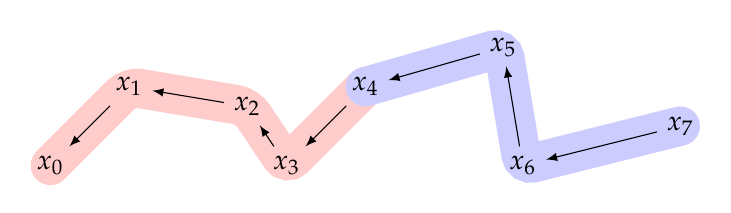
\begin{tikzpicture}
				\coordinate (a0) at (0,0);
				\coordinate (a1) at (1,1);
				\coordinate (a2) at (2.5,.75);
				\coordinate (a3) at (3,0);
				\coordinate (a4) at (4,1);
				\coordinate (a5) at (5.75,1.5);
				\coordinate (a6) at (6,0);
				\coordinate (a7) at (8,.5);
				%
				\draw[red!20,line width=5mm, rounded corners, cap=round] (a0) -- (a1) -- (a2) -- (a3) -- (a4);
				\draw[blue!20,line width=5mm, rounded corners, cap=round] (a4) -- (a5) -- (a6) -- (a7);
				%
				\foreach \i in {0,...,7}
				\node (e\i) at (a\i) {$x_\i$};
				\foreach \i in {0,...,6}{
						\edef\ipp{\fpeval{\i + 1}}
						\draw[latex-] (e\i) -- (e\ipp);
					}
			\end{tikzpicture}
		\end{center}
		\caption{Composizione di due morfismi \((x_0 \xot{e_1} x_1, x_1 \xot{e_2} x_2 ,x_2 \xot{e_3} x_3, x_3 \xot{e_4} x_4)\) e \((x_4 \xot{f_1} x_5,x_5 \xot{f_2} x_6, x_6 \xot{f_3} x_7)\) in \(\bfF[\ctG]\). Abbiamo usato il trucco di denotare le frecce da destra a sinistra qui, per rendere la composizione delle tue tuple la letterale concatenazione delle liste associate,
			\((\tup e4,)\circ (\tup f3,) = (\tup e4,,\tup f3,)\)
			(dando così a chi legge la libertà di decidere quale notazione sia meno confusionaria; purtroppo, secondo chi scrive, nessuna lo è davvero fino in fondo).}
		\label{fig:enter-label}
	\end{figure}
\end{example}
Dopo questa digressione veniamo a due esempi più elaborati, ma molto `concreti', di categorie dove gli oggetti sono numeri naturali:
\begin{hExample}[La categoria dei circuiti digitali]{tech}\label{ex_cat_circuiti}\index{Categoria!--- dei circuiti}
	La categoria \(\ctCirc\) ha
	\begin{itemize}
		\item per oggetti i numeri naturali \(0,1,2,\dots\);
		\item l'insieme dei morfismi \(\ctCirc(m,n)\) consiste dell'insieme delle funzioni \(\bbB^n\to \bbB^m\), dove \(\bbB=\{0,1\}\) è l'insieme dei \emph{Booleani}\footnote{L'insieme \(\bbB\) può essere interpretato come: l'insieme degli interi positivi modulo 2, l'insieme degli stati di un singolo bit di informazione; l'insieme \{sì, no\} delle risposte a una domanda; l'insieme \(\{-1,1\}\) dei \emph{segni} assunti dagli elementi dell'immagine di una funzione reale, l'insieme \{acceso, spento\} degli stati di un interruttore, eccetera.} e \(\bbB^0\defeq \{*\}, \bbB^{n+1}\defeq \bbB^n\times \bbB\) sono i prodotti cartesiani iterati di \(\bbB\) con sé stesso.
	\end{itemize}
	Si noti che ogni funzione Booleana \(f : \bbB^n\to\bbB^m\) risulta dal `prodotto' di \(m\) funzioni Booleane \emph{semplici} \(\tup fm, : \bbB^n\to\bbB\), di modo che
	\[f(\tup xn,)=(f_1(\tup xn,),\dots,f_m(\tup xn,)).\]
	Tra le funzioni Booleane semplici ci sono certamente le proiezioni canoniche \(\pi_{n,i} = \pi_i : \bbB^n\to\bbB :(\tup xn,)\mapsto x_i\), con le quali è possibile caratterizzare le \(f_i\) su menzionate: \(f_i = \pi_i\cmp f\); è anche possibile definire la mappa diagonale \(\Delta_m:\bbB\to\bbB^m\) come
	\[\Delta_m : x\mapsto (x,\dots,x)\quad m\text{ volte}\]
	cioè mediante le \(m\) funzioni semplici identità \(x\mapsto x\).

	Sull'insieme dei Booleani è possibile definire le operazioni logiche elementari di disgiunzione, congiunzione e negazione logica, che è possibile rappresentare graficamente con i seguenti diagrammi o `porte' logiche (note a qualsiasi ingegnere elettronico)
	\[\begin{circuitikz}
			\node[font=\tiny, xshift=-3cm, or port, fill=gray!10] (4,0) (or) {\(\text{OR}\)};
			\node[font=\tiny, and port, fill=gray!10] (0,0) (and) {\!\!\(\text{AND}\)};
			\node[font=\tiny, xshift=2.5cm, not port, fill=gray!10] (0,0) (not) {\!\!\(\text{NOT}\)};
		\end{circuitikz}\]
	\`E possibile comporre in serie le porte logiche, componendo i morfismi che esse rappresentano, e giustapporle in parallelo, allo stesso modo in cui è possibile considerare circuiti elettrici in serie e in parallelo per costruire strutture complesse come:
	\[
		\begin{circuitikz}[fill=gray!10]
			\draw (0,3) node[american and port] (A) {};
			\draw (A.out) -- ++(0.5,0) node[american or port,
				number inputs=2, anchor=in 1] (B) {};
			\draw (0,1.5) node[american or port] (C) {};
			\draw (C.out) |- (B.in 2);
			\draw (B.out) -- ++(.5,0) node[american not port,anchor=in 1] (D) {};
		\end{circuitikz}
	\]
	che rappresenta la funzione Booleana semplice
	\[(x,y,z,w)\mapsto \lnot((x\land y)\lor(z\lor w)).\]
\end{hExample}
Vale il seguente teorema:
\begin{theorem}\label{circ_thm}\index{Funzione Booleana}
	Ogni funzione Booleana semplice \(f :\bbB^n\to\bbB\) è esprimibile come composizione in serie e in parallelo di: proiezioni, mappe diagonali, congiunzioni e negazioni logiche.
\end{theorem}
Una maniera alternativa di esprimere questo risultato è affermare che l'insieme \(\{\text{AND},\text{OR}\}\) è \emph{funzionalmente completo} (o un \emph{insieme universale}) per il calcolo di porte logiche. Per una dimostrazione, si veda \cite[Teorema 1.4]{Crama2011}. In termini categoriali, stiamo affermando che un certo insieme di morfismi genera, insieme alle \(\pi_{n,1},\dots,\pi_{n,n}\) e \(\Delta_n\) per ogni \(n\ge 0\), l'intera categoria mediante le operazioni di prodotto e composizione.

Il capitolo \ref{chap_limiti_colimiti} e in particolare la nozione di prodotto, introdotta in \ref{chap_limiti_colimiti}, renderanno chiaro il ruolo fondamentale delle mappe \(\Delta_n,\tup{\pi}n,\) in questa e molte altre costruzioni.
\subsection{Categorie come universi}\label{ssec:categorie_universi}
Proseguiamo con degli esempi di categorie grandi, che giustificano l'intuizione per le categorie come `universi del discorso matematico', ossia come classi i cui costituenti sono collegati da relazioni reciproche.\footnote{Vale la pena una digressione: gli oggetti di una categoria $\ctC$ sono strettamente `tipati' dalla natura di $\ctC$, nel senso che, laddove è sempre possibile dire che `$S$ è un insieme', non è quasi mai possibile dire semplicemente `$X$ è un oggetto': \emph{di quale categoria?} In questo senso, la teoria delle categorie è strettamente affine alla teoria dei tipi, che si discosta molto dalla teoria degli insiemi proprio in virtù del fatto che i tipi non sono oggetti amorfi, tutti confrontabili uno con l'altro.} L'esempio fondamentale per tutta la sezione è \ref{ex_cat_insiemi}, la categoria di insiemi e funzioni. Usando questa categoria \(\ctSet\) come esempio paradigmatico, è possibile costruire
\begin{itemize}
	\item categorie di strutture algebriche (gruppi, anelli, algebre su un campo di base\dots); esempi di queste categorie sono \ref{ex_cat_monoidi}, e in generale \ref{ex_cat_sigma_strutture};
	\item categorie di strutture topologiche/ordinate (spazi topologici, insiemi parzialmente ordinati); esempi di queste categorie sono \ref{po_wo_to}, \ref{ex_cat_top};
\end{itemize}
e insieme a queste, molte altre. Esiste una dicotomia forte tra queste due classi di categorie, che sarà possibile apprezzare una volta introdotti più strumenti.

\`E tuttavia estremamente importante notare che
\begin{quote}
	Non tutte le categorie larghe si possono vedere come categorie di insiemi strutturati. Ad esempio, la categoria di \ref{ex_cat_hotop} non ha la proprietà di essere \emph{concreta} (si veda \ref{ssec:categorie_strutture}, \ref{def_costrutto}).
\end{quote}
\begin{example}[Insiemi e relazioni]\label{ex_cat_rels}\index{Categoria!--- delle relazioni}\index{Rel@\(\ctRel\)}
	La categoria \(\ctRel\) ha
	\begin{itemize}
		\item per oggetti gli insiemi, denotati con le lettere \(A,B,C,\dots\);
		\item per morfismi da \(A\) verso \(B\) tutte le \emph{relazioni} \(R\subseteq A\times B\), ossia i sottoinsiemi del prodotto cartesiano \(A\times B\).
	\end{itemize}
	Una relazione \(R\subseteq A\times B\) e una relazione \(S\subseteq B\times C\) si compongono nella relazione \(S\cmp R\) definita da
	\[(a,c)\in S\cmp R\iff \exists (b\in B) : ((a,b)\in R)\land ((b,c)\in S).\]
	Con questa definizione, si può mostrare che \(T\cmp(S\cmp R)=(T\cmp S)\cmp R\) e che la relazione diagonale \(\{(a,a)\mid a\in A\}\subseteq A\times A\) (ovvero la relazione \(a\,\Delta\,a'\iff a=a'\)) funge da elemento identità per la composizione così definita.
\end{example}
Nell'esempio appena fatto, l'ordine in cui si scrivono i fattori di un prodotto cartesiano è importante, perché se \(R : A\to B\) è una relazione, vogliamo che \(A\) ne sia il dominio, e \(B\) il codominio. \`E però vero che gli insiemi \(A\times B\) e \(B\times A\) sono in biiezione canonica, e quindi si potrebbe pensare di definire una categoria \(\ctRel'\) con gli stessi oggetti di \(\ctRel\), ma con morfismi da \(A\) verso \(B\) le relazioni \(R\subseteq B\times A\). In effetti, questa è la categoria opposta \(\ctRel^\op\) di \(\ctRel\) (si veda \ref{def_cat_opp}), e tra \(\ctRel^\op\) e \(\ctRel\) esiste un isomorfismo (si veda \ref{rel_autoduale}).
\begin{remark}\label{klext_delle_relazioni}\index{Relazione}\index{Relazione!estensione di ---}
	Ogni relazione \(R : A\to B\) induce una funzione \(R^* : \pow B\to \pow A\) nel modo che segue: un sottoinsieme \(U\subseteq B\) viene mandato in \(R^*U:=\{x\in A\mid \forall u\in U.(x,u)\in R\}\). In effetti, esiste una analoga funzione \(R_* : \pow A\to \pow B\), definita da \((V\subseteq A) \mapsto R_*V:= \{y\in B\mid \forall v\in V.(v,y)\in R\}\), e tra le due funzioni \(R^*, R_*\) sussiste la relazione
	\[V\subseteq R^*U \iff U\subseteq R_*V\label{aggiunti_in_disguise}\]
	dal momento che il lato sinistro è equivalente a \(\forall v\in V.\forall u\in U.(v,u)\in R\) e il lato destro a \(\forall u\in U.\forall v\in V.(v,u)\in R\). Nel capitolo \ref{cap_aggiunti} questo sarà un esempio elementare di una nozione importante, quella di \emph{aggiunzione} tra due categorie.
\end{remark}
\begin{remark}\label{diff_pres_cat_rel}\index{Categoria!--- delle relazioni}\index{Rel@\(\ctRel\)}
	L'osservazione precedente permette una differente presentazione per la categoria \(\ctRel\): gli oggetti di \(\ctRel\) sono ancora gli insiemi, ma una relazione \(R\subseteq X\times Y\) viene ora presentata come una \emph{funzione}
	\[\dmFun RX{\pow Y}\]
	definita mandando \(x\in X\) nell'insieme \(Rx = \{y\in Y\mid xRy\}\), e una tale relazione induce un'unica funzione \(\hat R : \pow X\to \pow Y\) definita da \(\hat R(U) = \bigcup_{x\in U}Rx = \{y\in Y\mid \exists x\in U,\, y\in Rx\}\), chiamata \emph{estensione di Kleisli} di \(R\) (il capitolo \ref{cap_monadi}, sulle monadi, chiarirà questa terminologia).

	La composizione di due relazioni \(R\subseteq X\times Y\) e \(S\subseteq Y\times Z\) è data dalla composizione \emph{di funzioni} \(\hat S\cmp R\), cioè
	\[
		x \mapsto \hat S(Rx) = \{z\in Z\mid \exists y\in Rx,\, ySz\}.
	\]
	Le proprietà generali di una estensione di Kleisli, che permettono di dimostrare che la definizione data soddisfa gli assiomi di categoria, sono le seguenti (tutte di facile dimostrazione, che lasciamo per esercizio):
	\begin{enumtag}{ek}
		\item \label{ek_1} per ogni insieme \(A\), esiste una \emph{relazione identica} \(\eta_A : A\to \pow A\), e \(\hat\eta_A\) è l'identità di \(\pow A\);
		\item \label{ek_2} se \(R : B\to \pow A\) è una relazione, allora \(\hat R\cmp \eta_B = R : B \to\pow A\);
		\item \label{ek_3} se \(R : B\to \pow A\) e \(S : C\to \pow B\) sono due relazioni, allora \(\hat S\cmp \hat R = \hat{S\cmp R} : C\to \pow A\).
	\end{enumtag}
\end{remark}
\begin{example}[Insiemi e funzioni]\label{ex_cat_insiemi}\index{Categoria!--- degli insiemi}
	\index{Categoria!--- degli insiemi finiti|see {--- degli insiemi}}\index{Insieme}
	La categoria \(\ctSet\) ha
	\begin{itemize}
		\item per oggetti gli insiemi, denotati con le lettere \(A,B,C\dots\);
		\item per morfismi da \(A\) verso \(B\) tutte le funzioni \(f : A\to B\), ossia tutte le relazioni \(F\subseteq A\times B\) con la proprietà che per ogni \(a\in A\) esiste un unico \(b\in B\) tale che \((a,b)\in F\) o, più formalmente, \(F\cap(\{a\}\times B)\) è un singoletto; l'elemento \(b\) in questione si denota \(f(a)\) o \(fa\) e l'insieme \(F = \{(a,fa)\mid a\in A\}\) è il \emph{grafico} o \emph{supporto} della funzione. Queste relazioni sono \emph{totali} (perché sono definite sull'intero dominio \(A\)) e \emph{a valore singolo}.
	\end{itemize}
	Due funzioni \(f : A\to B\), \(g : B\to C\) si compongono alla maniera delle relazioni (e la composizione è ancora una funzione, poiché l'intersezione \((G\cmp F)\cap (\{a\}\times C)\) consta del singoletto \(\{g(f(a))\}\)).

	La relazione diagonale è infine la (relazione sottostante alla) funzione identità.
\end{example}
Evidentemente, possiamo restringerci a considerare la categoria dei soli insiemi \emph{finiti} (così come la categoria \(\ctFRel\) delle relazioni tra insiemi finiti, che la contiene propriamente). Questo è il primo degli esempi motivanti fatti ad inizio capitolo, e in un senso evidente (che sarà precisato dalla definizione \ref{def_subcat}), \(\ctFRel\) è una \emph{sottocategoria} di \(\ctRel\) (e \(\ctFin\) è una sottocategoria di \(\ctSet\), che a sua volta è una sottocategoria di \(\ctRel\), sebbene in un modo non completamente banale).
\begin{example}[Categoria delle matrici in \(\bbF\)]\label{ex_cat_matrici}\index{Categoria!--- delle matrici}
	Per ogni anello con divisione \(\bbF\), posiamo definire la categoria \(\ctMat\) delle \emph{matrici a componenti in \(\bbF\)} come quella che ha
	\begin{itemize}
		\item per oggetti i numeri naturali \(0,1,2,\dots\);
		\item per morfismi \(n\to m\) le matrici con \(m\) righe ed \(n\) colonne a coefficienti in \(\bbF\), ossia:
		      \[\ctMat(n,m) = \matrici mn\bbF = \text{Lin}_{\bbF}(\bbF^n,\bbF^m)\]
		      dove \(\bbF^n:=\bbF \times\dots\times\bbF\) è il prodotto cartesiano iterato di \(\bbF\) con sé stesso \(n\) volte (quindi \(\bbF^0\) contiene il solo vettore nullo), e \(\text{Lin}_{\bbF}(\bbF^n,\bbF^m)\) è l'insieme delle funzioni \(\bbF\)-lineari \(\bbF^n\to\bbF^m\) (che scegliendo su dominio e codominio le basi canoniche, si identifica alle matrici a componenti in \(\bbF\) di taglia \(m\times n\)).
	\end{itemize}
	La composizione è il prodotto di matrici: se \(A : n\to m\) e \(B : m\to p\) sono matrici di entrate \((A_{ij}\mid 1\le i\le m,1\le j\le n)\) e \((B_{rs}\mid 1\le r\le p,1\le s\le m)\), la loro composizione \(BA : n\to p\) è la matrice \(BA\in \matrici pn\bbF\) definita da \((BA)_{ij} = \sum_{k=1}^m B_{ik}A_{kj}\).

	Questa operazione di composizione, come ricorda chiunque abbia studiato l'algebra lineare, è associativa, e la matrice identità \(I_n\in \matrici nn\bbF\) ne è l'elemento identità.
\end{example}
\begin{remark}\index{Vect@\(\ctVect\)}
	La categoria degli spazi vettoriali e mappe lineari, introdotta indirettamente in \ref{varie_categorie_nella_pratica}, e la categoria \(\ctMat\) ora definita, sono collegate in un senso preciso che sarà chiaro introducendo la nozione di \emph{scheletro} di una categoria in \ref{def_scheletro}: \(\ctMat\) si ottiene da \(\ctVect\) scegliendo un solo oggetto per ogni dimensione (dato che ogni \(\bbF\)-spazio vettoriale \(V\) di dimensione finita su \(\bbF\) è isomorfo ad un oggetto di \(\ctMat\)).
\end{remark}
Questo appena fatto è il secondo degli esempi motivanti fatti ad inizio capitolo.
\index{Categoria!--- di strutture algebriche}
\begin{example}\label{ex_cat_monoidi}\index{Omomorfismo!---di monoidi}
	Dati due monoidi \(M\) e \(N\), un \emph{omomorfismo di monoidi} \(f:M\to N\) è una funzione \(f:M\to N\) tale che
	\begin{itemize}
		\item \(f(e) = e\), cioè mappa l'elemento neutro di \(M\) in quello di \(N\);
		\item \(f(m\cdot m')=f(m)\cdot f(m')\) per ogni \(m,m'\in M\), cioè rispetta la moltiplicazione.
	\end{itemize}
	In particolare, se \(M\) ed \(N\) sono gruppi, un omomorfismo di monoidi è esattamente un omomorfismo di gruppi.
	Come si può facilmente verificare, l'identità su un monoide è un omomorfismo, e la composizione di omomorfismi è un omomorfismo.
	\begin{itemize}
		\item I monoidi e gli omomorfismi di monoidi formano la categoria \(\ctMon\).
		\item I gruppi e gli omomorfismi di gruppo formano la categoria \(\ctGrp\).
	\end{itemize}
\end{example}
L'idea da trattenere dopo questi primi esempi è che tutte le categorie di insiemi con operazioni che soddisfano, eventualmente, delle equazioni, forma una categoria; sebbene a volte non sia una questione banale scegliere la `giusta' nozione di omomorfismo tra strutture, ci affidiamo alla competenza che gli studi anteriori hanno dato a chi legge nel capire che, anche quando non abbiamo definito precisamente oggetti e morfismi, ci riferiamo alle categorie di strutture algebriche con le loro scelte `ovvie' di omomorfismo come funzione che rispetta (tutta) la struttura algebrica. Un'utile intuizione a riguardo è che in qualsiasi circostanza dove una classe di strutture possieda una nozione di omomorfismo che preserva la specifica di quella struttura, e tale che
\begin{itemize}
	\item l'identità è un omomorfismo;
	\item la composizione di due omomorfismi è ancora un omomorfismo;
\end{itemize}
si riesce a definire la classe degli oggetti e dei morfismi di una categoria.

L'\emph{algebra universale} si occupa di rendere preciso il concetto di `insieme dotato di operazioni', codificando una struttura algebrica mediante una \emph{funzione di arietà}:\footnote{Le parole \emph{arietà}, così come \emph{nullario} e \emph{unario} e \(n\)-ario (ma non binario, ternario, quaternario, etc.) sono retroformazioni che il lessico matematico ha introdotto a partire dal suffisso latino \emph{-\={a}rius, -\=aria, -\=arium}, usato per formare aggettivi a partire da nomi o numerali. Una operazione `\(n\)-aria' accetta \(n\) argomenti a dominio.} innanzitutto, si ricordi che una operazione \(n\)-aria su un insieme \(X\) consta di una funzione \(X\times X\times\dots\times X \to X\) dove il prodotto cartesiano è fatto \(n\) volte.
\begin{example}\label{ex_cat_sigma_strutture}\index{Categoria!---}
	Una \emph{segnatura algebrica} consiste di una coppia \((\Omega, a)\) dove \(\Omega\) è un insieme, e \(a : \Omega \to \bbN\) è una funzione detta \emph{funzione di arietà} che associa a ogni elemento \(\omega \in \Omega\) la sua arietà \(a(\omega)\ge 0\). Un \emph{modello} per una segnatura algebrica \((\Omega,a)\) consiste di un insieme \(X\) e di una funzione \(f_\bullet\) che associa a ogni \(\omega\in\Omega\) una operazione \(f_\omega : X^{a(\omega)} \to X\) di arietà \(a(\omega)\).

	Fissata una segnatura algebrica \((\Omega,a)\) possiamo definire la categoria \(\ctMod(\Omega,a)\) dei suoi modelli come segue:
	\begin{itemize}
		\item gli oggetti di \(\ctMod(\Omega,a)\) sono precisamente i modelli \((X,f_\bullet)\) di \((\Omega,a)\);
		\item fissati due modelli \((X,f_\bullet), (Y,g_\bullet)\) un \emph{omomorfismo} di modelli è una funzione \(h : X\to Y\) con la proprietà che per ogni \(\omega\in\Omega\) si abbia l'uguaglianza
		      \[h(f_\omega(\tup x{a(\omega)},)) = g_\omega(\tup {hx}{a(\omega)},)\]
		      o in termini diagrammatici, il seguente diagramma commuta.
		      \[
			      \begin{tikzcd}
				      X^{a(\omega)} \ar{r}{h^{a(\omega)}} \ar[d, "f_\omega"'] & Y^{a(\omega)} \ar{d}{g_\omega} \\
				      X \ar[r, "f"']& Y
			      \end{tikzcd}
		      \]
	\end{itemize}
\end{example}
\`E un esercizio tedioso nella manipolazione delle tuple ordinate, ora, dimostrare che gli assiomi di categoria sono tutti soddisfatti. Un esercizio analogamente tedioso è di trovare segnature algebriche opportune che esprimono le categorie dei gruppi, dei monoidi, degli anelli e degli spazi vettoriali ecc.\ come esempi particolari di categorie di modelli di una segnatura algebrica.\footnote{Tedioso, e a volte non proprio banale: ad esempio, come si descrivono le operazioni di moltiplicazione per scalare in uno spazio vettoriale usando la definizione di segnatura algebrica? Si noti anche che la richiesta che un omomorfismo di modelli rispetti \emph{tutti} gli elementi della segnatura a volte è ridondante: ogni omomorfismo di gruppi \(f : G\to H\) manda l'identità del dominio nell'identità del codominio perché \(f(e_G)\) deve essere un elemento idempotente di \(H\), e preserva gli inversi come corollario.}
\begin{remark}\label{varie_categorie_nella_pratica}\index{Categoria!---e di strutture algebriche}
	Categorie di modelli come in \ref{ex_cat_sigma_strutture} sono tra le più comuni da considerare nella pratica matematica: i monoidi e i loro omomorfismi, i gruppi e i loro omomorfismi (tra essi, la sottocategoria dei gruppi abeliani), gli anelli e i loro omomorfismi (tra essi, la sottocategoria degli anelli commutativi), gli spazi vettoriali su un qualsiasi campo \(k\) e le funzioni \(k\)-lineari, formano tutte esempi di categorie, che denotiamo con \(\ctMon\), \(\ctGrp\), \(\ctAb\), \(\ctRing\), \(\ctcRing\), \(\ctVect[k]\),\dots
\end{remark}
\begin{example}[Categoria dei multidigrafi]\label{ex_cat_grafi}\index{Categoria!--- dei grafi}
	Questo esempio rende precise alcune osservazioni fatte in precedenza, \ref{ex_cat_doppiafreccia} e \ref{ex_cat_libera}. La categoria \(\ctdGph\) dei grafi è così definita:
	\begin{itemize}
		\item gli oggetti di \(\ctdGph\) sono i grafi, o più precisamente i \emph{multidigrafi}: un (multidi)grafo \(\ctG = (E,V,s,t)\) consiste di una coppia di insiemi \(E,V\) dotati di due funzioni \(s,t : E\toto V\) che associano ad ogni \emph{lato} \(e\in E\) una coppia ordinata di \emph{vertici} \(s(e),t(e)\in V\) detti il suo dominio o \emph{source} e il suo codominio o \emph{target}.
		\item Un omomorfismo di (multidi)grafi \((f_E,f_V) : (E,V,s,t)=\ctG\to\ctG'= (E', V',s',t')\) consiste in una coppia di funzioni \(f_E, f_V\) tali che
		      \begin{gather*}
			      s'\cmp f_E = f_V\cmp s\\
			      t'\cmp f_E = f_V\cmp t
		      \end{gather*}
		      o in termini diagrammatici, tali che i due quadrati seguenti siano commutativi,
		      % https://q.uiver.app/#q=WzAsOCxbMCwwLCJFIl0sWzAsMSwiViJdLFsxLDAsIkUnIl0sWzEsMSwiViciXSxbMiwwLCJFIl0sWzMsMCwiRSciXSxbMiwxLCJWIl0sWzMsMSwiViciXSxbMCwyLCJmX0UiXSxbMiwzLCJzJyJdLFsxLDMsImZfViIsMl0sWzAsMSwicyIsMl0sWzQsNSwiZl9FIl0sWzYsNywiZl9WIl0sWzUsNywidCciXSxbNCw2LCJ0IiwyXV0=
		      \[\begin{tikzcd}
				      E & {E'} & E & {E'} \\
				      V & {V'} & V & {V'}
				      \arrow["{f_E}", from=1-1, to=1-2]
				      \arrow["{s'}", from=1-2, to=2-2]
				      \arrow["{f_V}"', from=2-1, to=2-2]
				      \arrow["s"', from=1-1, to=2-1]
				      \arrow["{f_E}", from=1-3, to=1-4]
				      \arrow["{f_V}"', from=2-3, to=2-4]
				      \arrow["{t'}", from=1-4, to=2-4]
				      \arrow["t"', from=1-3, to=2-3]
			      \end{tikzcd}\]
		      cosicché \((f_E,f_V)\) commutano con le funzioni di source e target.
	\end{itemize}
	Si noti che questo significa che questo impone precisamente che per ogni \(e\in E\), \(f_E(e)\) sia un lato in \(E'\) di vertici \(f_V(se), f_V(te)\) rispettivamente.
\end{example}
Evidentemente, possiamo scrivere \(e : x\to y\) per denotare in maniera compatta il fatto che \(e \in E\) è un lato tale che \(se=x,te=y\); allora un omomorfismo di multidigrafi è tale che se \(e : x\to y\), allora \(f_Ee : f_Vx\to f_Vy\).
\begin{example}[Categoria dei grafi]\label{ex_cat_grafi_nondiretti}\index{Categoria!--- dei grafi non diretti}
	In maniera simile possiamo definire la categoria \(\ctGph\) dei grafi non diretti; un grafo non diretto è un insieme \(V\) di vertici, su cui sia definita una relazione \(E\subseteq V\times V\), simmetrica e irriflessiva (cioè \(\forall v\in V.(v,v)\notin E\)).

	Un omomorfismo di grafi non diretti è una funzione tra i vertici \(f_V : V\to V'\) compatibile con le relazioni \(E,E'\): se \((u,v)\in E\), allora \((fu,fv)\in E'\).
\end{example}
\begin{example}\label{ex_cat_ordini}\index{Categoria!--- di insiemi ordinati}\index{Preordine}
	Si ricordi da \ref{prelim_def_preset} che un \emph{insieme preordinato} è un insieme \(P\) dotato di una relazione riflessiva e transitiva \(\le\) che si dice la \emph{(relazione d')ordine} su \(P\); una funzione \(f : (P,\le)\to (Q,\preceq)\) si dice \emph{monotòna} o si dice che \(f\) \emph{preserva l'ordine} se vale
	\[\forall x,y(x\le y\Rightarrow fx\preceq fy).\]

	La categoria \(\ctPOrd\) ha per oggetti e morfismi gli insiemi preordinati e le funzioni monotòne. Chiaramente, l'identità \(\id_P : (P,\le)\to (P,\le)\) è una funzione monotòna, e la composizione di due funzioni monotòne resta monotòna.

	\`E tuttavia importante che l'ordine su \(P\) sia \emph{lo stesso} affinché l'identità sia monotòna: infatti, ogni insieme \(P\) può essere dotato dell'ordine \emph{banale} (dove \(x \mathrel{\le^\delta} y\) se e solo se \(x=y\)) e dell'ordine \emph{caotico} (dove \(x\mathrel{\le^\chi} y\) per ogni \(x,y\in P\)). Se \(P\) ha almeno due elementi, la funzione identità \((P,\le^\chi)\to (P,\le^\delta)\) non è, chiaramente, monotòna.
\end{example}
\begin{remark}[po, wo e to]\label{po_wo_to}\index{Ordine parziale}\index{Ordinale}
	Una sottoclasse importante di preordini si ottiene imponendo che \(\le\) sia una relazione antisimmetrica; in tal caso il preordine \((P,\le)\) si dice un \emph{insieme parzialmente ordinato} (in inglese, \emph{p}artially \emph{o}rdered \emph{set} o brevemente \emph{poset}). La categoria \(\ctPos\) ha per oggetti i poset e per morfismi le stesse funzioni monotòne di \ref{ex_cat_ordini}.

	Un'altra sottocategoria importante di \(\ctPOrd\) è quella degli insiemi \emph{totalmente ordinati} o \emph{toset}, dove tutti gli elementi sono confrontabili tra loro:
	\[\forall x,y\in P.((x\le y)\lor (y\le x));\]
	da ultimo, una ulteriore sottocategoria importante di \(\ctPOrd\) è quella degli insiemi \emph{bene ordinati} (in inglese, \emph{w}ell \emph{o}rdered sets, o brevemente \emph{wosets}), dove ogni sottoinsieme non vuoto ammette un elemento minimo. Se \((P,\le)\) è un woset, si dice anche che \(P\) è un \emph{buon ordine} rispetto a \(\le\).
\end{remark}
\begin{example}\label{ex_cat_ordinali}\index{Categoria!--- degli ordinali}
	Ricordiamo che un insieme \(X\) si dice \emph{transitivo} se una qualsiasi delle seguenti condizioni equivalenti è soddisfatta:
	\begin{itemize}
		\item \(x\in X\Rightarrow x\subseteq X\);
		\item \(X\subseteq \pow X\);
		\item \(\bigcup X\subseteq X\).
	\end{itemize}
	Un insieme \(X\) si dice un \emph{ordinale} se è transitivo e se ogni sottoinsieme non vuoto \(S\subseteq X\) ammette un elemento \(\in\)-minimo, cioè se \(X\) è bene ordinato dalla relazione \(\in\).

	La categoria \(\ctOrd\) ha per oggetti gli ordinali e per morfismi \(X\to Y\) le funzioni monotòne.
\end{example}
L'importanza della categoria degli ordinali sarà più evidente quando nella sezione \ref{sec_funtori} introdurremo la definizione di funtore. Per il momento, ci limitiamo ad alcune osservazioni.
\begin{remark}\label{rmk_delta_e_deltaPlus}\index{Ordinale!--- finito}\index{Categoria!--- dei simplessi}
	Se \([n]=\{\iter[0] n\}\) è un insieme finito, l'ordinamento \(\{\iter[0][<]n\}\) lo rende un woset nel senso di \ref{po_wo_to}, e quindi \(\Delta[n]\) è in maniera naturale un oggetto di \(\ctPos\), ma anche di \(\ctOrd\); insieme alle funzioni monotòne tra questi insiemi finiti, ciò identifica la sottocategoria di \(\ctOrd\) generata da tutte le catene generiche \(\Delta[n]\) di \ref{ex_cat_catena} con la sottocategoria \(\ctFOrd\) di tutti gli ordinali finiti e non vuoti.
	\begin{itemize}
		\item Una notazione alternativa e più comune, mutuata dalla topologia algebrica, per \(\ctFOrd\)	è \(\bsDelta\) (la lettera greca delta maiuscola), che viene chiamata la categoria dei \emph{simplessi}. In \ref{def_real_geom} vedremo che ogni simplesso ammette una \emph{realizzazione topologica} come sottospazio \(\Delta^n\subseteq\bbR^{n+1}\), e questo motiva l'interesse geometrico per questi oggetti. Di volta in volta sceglieremo quale notazione adottare: se ci riferiamo alla categoria degli ordinali finiti con un'applicazione geometrica in mente, useremo la notazione \(\bsDelta\); se invece ci riferiamo alla categoria degli ordinali finiti come esempio di categoria di insiemi ordinati, useremo la notazione \(\ctFOrd\). \`E però importante notare che \(\bsDelta\) e \(\ctFOrd\) sono sinonimi perfetti.
		\item Per la categoria di \emph{tutti} gli ordinali finiti, anche quello vuoto, si usa la notazione \(\bsDelta_+\), che viene chiamata la categoria dei \emph{simplessi aumentati} (in questo senso, si capisce cosa sia la categoria \(\ctFOrd_+\), ma questa notazione non appare mai).
	\end{itemize}
\end{remark}
\begin{figure}[h]
	\begin{center}
		\begin{tikzpicture}[
				x=4em, y=4em,
				wrap/.style={fill=black!5, rounded corners},
				edge/.style={-latex},
				0simplex/.style={font=\scriptsize,inner sep=2pt},
			]
			\begin{scope}[xshift=0em,yshift=0.433*5em]
				\node[0simplex] (0D0) at (0.0,0) {0};
			\end{scope}
			\begin{scope}[xshift=4em,yshift=0.433*5em]
				\node[0simplex] (1D0) at (0.0,0) {0};
				\node[0simplex] (1D1) at (1.0,0) {1};
				\draw[edge, ibmMagenta] (1D0) -- (1D1);
			\end{scope}
			\begin{scope}[xshift=13em]
				\node[0simplex] (2D0) at (0.0,0) {0};
				\node[0simplex] (2D1) at (1.0,0) {1};
				\node[0simplex] (2D2) at (0.5,0.866) {2};
				\draw[edge, ibmMagenta] (2D0) -- (2D1);
				\draw[edge] (2D0) -- (2D2);
				\draw[edge, ibmMagenta] (2D1) -- (2D2);
			\end{scope}
			\begin{scope}[xshift=22em]
				\node[0simplex] (3D0) at (0.0,0) {0};
				\node[0simplex] (3D1) at (1.0,0) {1};
				\node[0simplex] (3D2) at (0.5,0.866) {2};
				\node[0simplex] (3D3) at (0.5,0.3) {3};
				\draw[edge,ibmMagenta] (3D0) -- (3D1);
				\draw[edge] (3D0) -- (3D2);
				\draw[edge,ibmMagenta] (3D1) -- (3D2);
				\draw[edge] (3D0) -- (3D3);
				\draw[edge] (3D1) -- (3D3);
				\draw[edge,ibmMagenta] (3D2) -- (3D3);
			\end{scope}
			\begin{scope}[on background layer]
				\path node[wrap, fit=(0D0)] (W0) {};
				\path node[wrap, fit=(1D0)(1D1)] (W1) {};
				\path node[wrap, fit=(2D0)(2D1)(2D2)] (W2) {};
				\path node[wrap, fit=(3D0)(3D1)(3D2)(3D3)] (W3) {};
				\node [below=2.5em of W0] (L) {$\Delta[0]$};
				\node at (L -| W1) {$\Delta[1]$};
				\node at (L -| W2) {$\Delta[2]$};
				\node at (L -| W3) {$\Delta[3]$};
			\end{scope}
		\end{tikzpicture}
	\end{center}
	\caption{Le categorie \(\Delta[0], \dots,\Delta[3]\) già viste in \ref{ex_cat_catena}, con le loro \emph{spine} in evidenza; la spina di un simplesso è la catena di frecce \(0\to 1\to\cdots\to n\) che genera, per composizione, tutte le altre frecce di \(\Delta[n]\).}
	\label{fig:spines}
\end{figure}
\begin{hRemark}[Combinatoria della categoria \(\bsDelta\)]{skip}\label{rmk_combinatoria_simplessi}\index{Categoria!--- dei simplessi}
	La categoria \(\bsDelta\) possiede una sottoclasse di morfismi che generano tutti gli altri per composizione. Tra tutte le mappe monotòne \(f : [n]\to [m]\) in \(\bsDelta\) possiamo distinguere le \(n+1\) funzioni \emph{iniettive} \(\delta_n^i : [n-1]\mono [n]\) che evitano l'elemento \(i=\iter[0]n\), e le \(n+1\) funzioni \emph{suriettive} \(\sigma_n^j : [n+1]\epi [n]\) che assumono due volte il valore  \(j=\iter[0]m\):
	\[
		\delta_n^i(k) =
		\begin{cases}
			k,   & k < i    \\
			k+1, & k \geq i
		\end{cases}
		\quad \quad
		\sigma_n^j (k) =
		\begin{cases}
			k,   & k \leq j \\
			k-1, & k > j
		\end{cases}
		\quad \text{per} \quad 0 \leq j\leq n.
	\]
	\index{Insieme simpliciale}\index{Insieme!--- simpliciale}
	Per ogni \(n\ge 0\), \(\{\delta_n^0,\dots,\delta_n^{n+1}\}\) sono dette le \emph{cofacce} di \([n]\), e \(\{\sigma_n^0,\dots, \sigma_n^n\}\) le \emph{codegenerazioni} di \([n]\). Raffiguriamo alcune mappe di cofaccia e codegenerazione in \autoref{fig:cofa} e \ref{fig:code}. Tali funzioni soddisfano le seguenti relazioni, dette \emph{identità cosimpliciali}:
	\begin{gather*}
		\delta_n^j \cmp \delta_{n-1}^i = \delta_n^i \cmp \delta_{n-1}^{j-1}, \quad i < j\\
		\sigma_n^j \cmp \sigma_{n+1}^i = \sigma_n^i \cmp \sigma_{n+1}^{j+1}, \quad i \leq j\\
		\sigma_n^j \cmp \delta_{n+1}^i =
		\begin{cases}
			\delta_n^i \cmp \sigma_{n-1}^{j-1}, & i < j      \\
			\id,                                & i = j, j+1 \\
			\delta_n^{i-1} \cmp \sigma_{n-1}^j, & i > j+1.
		\end{cases}
	\end{gather*}
	Ogni freccia di \(\Hom\bsDelta([n],[m])\) si può scrivere, in maniera essenzialmente unica, come composizione di alcune mappe di codegenerazione, seguite da alcune mappe di cofaccia; l'idea è di fattorizzare \(f\) lungo la sua immagine (dotata dell'ordine indotto),
	\[\xymatrix{
			[n]\ar[rr]^f\ar[dr]_e &&	[m] \\
			& \im(f) \ar[ur]_m
		}\]
	e conseguentemente immergere quest'ultima nel codominio. La funzione suriettiva \(e\) è composizione di codegenerazioni (precisamente quelle determinate dai valori che \(f\) assume molteplici volte), e la funzione iniettiva \(m\) è composizione di alcune cofacce (precisamente quelle determinate dai valori che \(f\) non assume).
\end{hRemark}
\begin{figure}
	\begin{center}
		\begin{tikzpicture}[x=.5cm]
			\tikzset{
				fitbg/.style={inner sep=0pt, fill=gray!50, opacity=0.5}
			}
			\drawChain{3}[up]
			\begin{pgfonlayer}{background}
				\node[fitbg,fit=(0up)(3up)] {};
			\end{pgfonlayer}
			\begin{scope}[yshift=-1cm]
				\drawChain{4}[down]
				\begin{pgfonlayer}{background}
					\node[fitbg,fit=(1down)(4down)] {};
				\end{pgfonlayer}
			\end{scope}
			\foreach \i/\j in {0/1,1/2,2/3,3/4}
			\draw[-latex] (\i up) -- (\j down);
			\begin{scope}[xshift=3cm]
				\drawChain{3}[up]
				\begin{pgfonlayer}{background}
					\node[fitbg,fit=(0up)] {};
					\node[fitbg,fit=(1up)(3up)] {};
				\end{pgfonlayer}
				\begin{scope}[yshift=-1cm]
					\drawChain{4}[down]
					\begin{pgfonlayer}{background}
						\node[fitbg,fit=(0down)] {};
						\node[fitbg,fit=(2down)(4down)] {};
					\end{pgfonlayer}
				\end{scope}
				\foreach \i/\j in {0/0,1/2,2/3,3/4}
				\draw[-latex] (\i up) -- (\j down);
				\begin{scope}[xshift=3cm]
					\drawChain{3}[up]
					\begin{pgfonlayer}{background}
						\node[fitbg,fit=(0up)(1up)] {};
						\node[fitbg,fit=(2up)(3up)] {};
					\end{pgfonlayer}
					\begin{scope}[yshift=-1cm]
						\drawChain{4}[down]
						\begin{pgfonlayer}{background}
							\node[fitbg,fit=(0down)(1down)] {};
							\node[fitbg,fit=(3down)(4down)] {};
						\end{pgfonlayer}
					\end{scope}
					\foreach \i/\j in {0/0,1/1,2/3,3/4}
					\draw[-latex] (\i up) -- (\j down);
					\begin{scope}[xshift=3cm]
						\drawChain{3}[up]
						\begin{pgfonlayer}{background}
							\node[fitbg,fit=(0up)(2up)] {};
							\node[fitbg,fit=(3up)] {};
						\end{pgfonlayer}
						\begin{scope}[yshift=-1cm]
							\drawChain{4}[down]
							\begin{pgfonlayer}{background}
								\node[fitbg,fit=(0down)(2down)] {};
								\node[fitbg,fit=(4down)] {};
							\end{pgfonlayer}
						\end{scope}
						\foreach \i/\j in {0/0,1/1,2/2,3/4}
						\draw[-latex] (\i up) -- (\j down);
						\begin{scope}[xshift=3cm]
							\drawChain{3}[up]
							\begin{pgfonlayer}{background}
								\node[fitbg,fit=(0up)(3up)] {};
							\end{pgfonlayer}
							\begin{scope}[yshift=-1cm]
								\drawChain{4}[down]
								\begin{pgfonlayer}{background}
									\node[fitbg,fit=(0down)(3down)] {};
								\end{pgfonlayer}
							\end{scope}
							\foreach \i/\j in {0/0,1/1,2/2,3/3}
							\draw[-latex] (\i up) -- (\j down);
						\end{scope}
					\end{scope}
				\end{scope}
			\end{scope}
		\end{tikzpicture}
	\end{center}
	\caption{Le cinque mappe di cofaccia \(\delta_4^0,\dots,\delta_4^4 : [3]\mono [4]\) in \(\bsDelta\). Ciascun segmento \(\{\iter[0][<]{i-1}\}\) viene mappato in sé stesso da \(\delta_n^i\); i \(k\) maggiori o uguali di \(i\) vengono mappati in \(k+1\).}
	\label{fig:code}
\end{figure}

\begin{figure}
	\begin{center}
		\begin{tikzpicture}[x=.5cm]
			\tikzset{
				fitbg/.style={inner sep=0pt, fill=gray!50, opacity=0.5}
			}
			\drawChain{4}[up]
			\begin{pgfonlayer}{background}
				\node[fitbg,fit=(0up)(1up)] {};
				\node[fitbg,fit=(2up)(4up)] {};
			\end{pgfonlayer}
			\begin{scope}[yshift=-1cm]
				\drawChain{3}[down]
				\begin{pgfonlayer}{background}
					\node[fitbg,fit=(0down)] {};
					\node[fitbg,fit=(1down)(3down)] {};
				\end{pgfonlayer}
			\end{scope}
			\foreach \i/\j in {0/0,1/0,2/1,3/2,4/3}
			\draw[-latex] (\i up) -- (\j down);
			\begin{scope}[xshift=3cm]
				\drawChain{4}[up]
				\begin{pgfonlayer}{background}
					\node[fitbg,fit=(0up)] {};
					\node[fitbg,fit=(1up)(2up)] {};
					\node[fitbg,fit=(3up)(4up)] {};
				\end{pgfonlayer}
				\begin{scope}[yshift=-1cm]
					\drawChain{3}[down]
					\begin{pgfonlayer}{background}
						\node[fitbg,fit=(0down)] {};
						\node[fitbg,fit=(1down)] {};
						\node[fitbg,fit=(2down)(3down)] {};
					\end{pgfonlayer}
				\end{scope}
				\foreach \i/\j in {0/0,1/1,2/1,3/2,4/3}
				\draw[-latex] (\i up) -- (\j down);
				\begin{scope}[xshift=3cm]
					\drawChain{4}[up]
					\begin{pgfonlayer}{background}
						\node[fitbg,fit=(0up)(1up)] {};
						\node[fitbg,fit=(2up)(3up)] {};
						\node[fitbg,fit=(4up)] {};
					\end{pgfonlayer}
					\begin{scope}[yshift=-1cm]
						\drawChain{3}[down]
						\begin{pgfonlayer}{background}
							\node[fitbg,fit=(0down)(1down)] {};
							\node[fitbg,fit=(2down)] {};
							\node[fitbg,fit=(3down)] {};
						\end{pgfonlayer}
					\end{scope}
					\foreach \i/\j in {0/0,1/1,2/2,3/2,4/3}
					\draw[-latex] (\i up) -- (\j down);
					\begin{scope}[xshift=3cm]
						\drawChain{4}[up]
						\begin{pgfonlayer}{background}
							\node[fitbg,fit=(0up)(2up)] {};
							\node[fitbg,fit=(3up)(4up)] {};
						\end{pgfonlayer}
						\begin{scope}[yshift=-1cm]
							\drawChain{3}[down]
							\begin{pgfonlayer}{background}
								\node[fitbg,fit=(0down)(2down)] {};
								\node[fitbg,fit=(3down)] {};
							\end{pgfonlayer}
						\end{scope}
						\foreach \i/\j in {0/0,1/1,2/2,3/3,4/3}
						\draw[-latex] (\i up) -- (\j down);
					\end{scope}
				\end{scope}
			\end{scope}
		\end{tikzpicture}
	\end{center}
	\caption{Le quattro mappe di codegenerazione \(\sigma_4^0,\dots,\sigma_4^4 : [4]\mono [3]\) in \(\bsDelta\). Ciascun valore \(i=\iter[0] n\) viene assunto due volte da \(\sigma_n^i\).}
	\label{fig:cofa}
\end{figure}
\begin{remark}\index{Universo}\index{Ordinale}\label{tipi_di_ordinaly}
	Senza un assioma dedicato a tale scopo, non si possono generare ordinali più grandi di quelli finiti; al contrario, assumendo che esista almeno un insieme \emph{induttivo} \(N\) (cioè tale che, se \(x\in N\), allora \(x^+:=x\cup\{x\}\in N\)), possiamo `accedere' a ordinali più grandi, e da qui generarne di \emph{molto} grandi (abbastanza da far sì che la categoria \(\ctOrd\) abbia una classe propria di oggetti).

	Questa è una maniera un po' semplificata di introdurre l'ordinale \(\omega\) ottenuto come `limite' di tutti gli ordinali finiti \([n]\): rinviamo chi legge a un corso di logica elementare per approfondire la questione in modo più tecnico, e ci limitiamo a osservare che la dicotomia importante nella definizione di un numero ordinale è la seguente: un ordinale \(\alpha\in\ctOrd_0\) può essere di due tipi: un \emph{successore}, se esiste \(\beta\) tale che \(\alpha=\beta^+\), e un \emph{limite} se, invece, \(\alpha=\bigcup\alpha=\sup\{\gamma\mid \gamma < \alpha\}\).
\end{remark}
\begin{remark}\label{es_catena_trans}\index{Ordinale!induzione con ---i}
	L'importanza degli ordinali risiede nella possibilità di dare \emph{definizioni per induzione} (finita o transfinita) mediante essi: se \(\ctC\) è una classe, una funzione di classe \(H : \ctOrd_0\to\ctC\) si dice \emph{continua} se è univocamente determinata dalla specifica
	\begin{itemize}
		\item di un elemento \(H(0)\in\ctC\) detto base dell'induzione;
		\item di una maniera di calcolare \(H(x^+)\) in funzione di \(H(0), H(1),\dots,H(x)\); questo è il \emph{passo induttivo} della costruzione;
		\item di una maniera di calcolare il `passo limite' dell'induzione, \(H(\lambda)\), in termini di \(H(\gamma)\) per tutti i \(\gamma < \lambda\).
	\end{itemize}
	Una costruzione simile si apprezzerà una volta introdotta la definizione di funtore, dato che una maniera di formalizzare le successioni
	\[\begin{tikzcd}
			A_0 \ar[r] & A_1 \ar[r] & A_2 \ar[r] & \cdots \ar[r] & A_\lambda
		\end{tikzcd}\]
	\emph{eventualmente infinite} di morfismi contigui in una categoria \(\ctC\) sarà esattamente definendole come funtori \(\ctOrd_{\le\lambda}\funto \ctC\).
\end{remark}
\begin{hExample}[Spazi topologici]{fund}\label{ex_cat_top}\index{Categoria!--- di spazi topologici}
	Ricordiamo che uno \emph{spazio topologico} è un insieme \(X\) dotato di una \emph{topologia}, cioè una collezione \(\tau_X\) di sottoinsiemi di \(X\), chiamati gli \emph{aperti}, contenente l'insieme vuoto e \(X\) stesso, e chiusa rispetto alle intersezioni finite e a tutte le unioni.
	Dati due spazi topologici \((X,\tau_X)\) e \((Y,\tau_Y)\), una funzione \(f:X\to Y\) è continua per le topologie \(\tau_X\) e \(\tau_Y\) se per ogni aperto \(V\in\tau_Y\), la sua preimmagine \(f^{-1}(V)\) è un aperto di \(\tau_X\).
	Gli spazi topologici e le funzioni continue tra loro formano la categoria \(\ctTop\).
\end{hExample}
\begin{hExample}[Spazi topologici e classi di omotopia]{skip}\index{Categoria!--- dell'omotopia}\index{Equivalenza!--- a omotopica}\label{ex_cat_hotop}
	La categoria \(\ctHoTop\) detta \emph{categoria dell'omotopia (di spazi topologici)} è così definita:
	\begin{itemize}
		\item gli oggetti di \(\ctHoTop\) sono gli spazi topologici di \ref{ex_cat_top};
		\item una freccia tra due spazi topologici \(X,Y\) è una classe di omotopia di mappe continue \(X\to Y\), dove la relazione di omotopia in \(\ctTop(X,Y)\) è definita così: due mappe continue \(f,g : X\to Y\) sono omotope (l'accento è sulla prima \emph{o}) quando esiste una funzione continua \(H : X \times [0,1] \to Y\) tale che \(H(x,0) = f(x)\) e \(H(x,1)=g(x)\) per ogni \(x\in X\). Questo si denota con \(f\simeq_H g\) o brevemente con \(f\simeq g\) (quando è univoco, o ovvio, come costruire \(H\) a partire dal contesto).
	\end{itemize}
	La composizione di classi di omotopia di mappe continue è definita grazie al fatto che l'omotopia tra mappe è una congruenza su ogni \(\ctTop(X,Y)\) (cioè, se \(f\simeq g\), allora \(h\cmp f\cmp k\simeq h\cmp g\cmp k\)): si veda anche \ref{fun_ex_omoto_omolo} più avanti.
\end{hExample}
\begin{hExample}[La categoria degli spazi di misura]{skip}\label{ex_cat_meas}\index{Categoria!--- degli spazi misurabili}
	Nel definire una categoria appropriata dove fare teoria della misura, si vorrebbe prendere come oggetti le coppie \((X, \fkM)\), dove \(X\) è un insieme e \(\fkM\) è una \(\sigma\)-algebra di sottoinsiemi misurabili di \(X\). Le frecce \((X, \fkM) \to (X', \fkM')\) allora dovrebbero essere funzioni \(f: X \to X'\) tra gli insiemi sottostanti, tali che per ogni \(E \in \fkM'\) si abbia \(f^{-1}(E) \in \fkM\), ossia le controimmagini di insiemi misurabili sono misurabili. Questo è del tutto in linea con ciò che si fa in topologia, e si apprende in qualsiasi introduzione alla teoria della misura.

	Un problema insito in questo approccio, che però la nozione di continuità non pone, è l'intuizione dietro gli elementi di \(\fkM\), che si pensano come insiemi `grandi' o `piccoli' a seconda della loro misura.\footnote{\dots Laddove gli aperti \(U\) di una topologia si pensano come regioni che, per ogni \(x\in U\), affermano che un altro \(y\in U\) è `vicino' a \(x\), a prescindere da quanto \(U\) sia `grande'.} Formulare un teorema non banale di teoria della misura usando questa categoria è molto arduo, perché la nozione di \emph{insieme trascurabile} compare in modo rilevante in tutti i principali risultati di teoria della misura. Inoltre, in teoria della misura è una prassi generale \emph{identificare} funzioni che differiscono su un insieme di misura \(0\), cioè considerare non le funzioni \(f,f' : X\to X'\) vere e proprie, ma le classi di equivalenza rispetto alla relazione
	\[f\sim g \iff \{x\in X\mid f(x)\ne g(x)\} \text{ ha misura } 0\]
	Per risolvere il problema, la prassi è di definire una categoria \(\ctMeas\) i cui oggetti sono \emph{terne} \((X, \fkM, \fkN)\), dove \(X\) e \(\fkM\) sono come sopra, e \(\fkN \subset \fkM\) è un \emph{\(\sigma\)-ideale di insiemi trascurabili}. (Un \(\sigma\)-ideale è una \(\sigma\)-algebra che in più è chiusa rispetto al passaggio a sottoinsiemi; ciò riflette il fatto che i sottoinsiemi di insiemi di misura \(0\) hanno anch'essi misura \(0\).) Osserviamo che i dati contenuti in \(N\) codificano esattamente le stesse informazioni di una \emph{classe di misure}, cioè di una classe di equivalenza di misure su \((X, M)\) rispetto alla seguente relazione di equivalenza: \(\mu \sim \nu\) se \(\mu \ll \nu\) e \(\nu \ll \mu\).

	I morfismi \((X, \fkM, \fkN) \to (X', \fkM', \fkN')\) sono ora classi di equivalenza di funzioni \(f: X \to X'\) tali che \(f^{-1}E \in \fkM'\) per ogni \(E\in \fkM\), e \(f^{-1}V \in \fkN'\) per ogni \(V\in \fkN\). La relazione di equivalenza data dal differire su un insieme trascurabile è compatibile con la composizione di funzioni: se \(f \sim g\) per alcune
	\[
		f,g : (X_1, \fkM_1, \fkN_1) \to (X_2, \fkM_2, \fkN_2),
	\]
	allora \(f\cmp e \sim g\cmp e\) per ogni \(e: (X_0, \fkM_0, \fkN_0) \to (X_1, \fkM_1, \fkN_1)\) e \(h\cmp f \sim h\cmp g\) per ogni \(h: (X_2, \fkM_2, \fkN_2) \to (X_3, \fkM_3, \fkN_3)\).
\end{hExample}
Tutte le categorie considerate in precedenza hanno il seguente schema: gli oggetti sono insiemi dotati di struttura aggiuntiva, i morfismi sono funzioni che preservano tale struttura. La categoria \(\ctMeas\) non è di questo tipo perché identifichiamo funzioni che differiscono su un insieme di misura zero. In particolare, si può dimostrare che dato un morfismo in \(\ctMeas\), non esiste modo di scegliere una funzione rappresentante in modo che tali scelte rispettino la composizione (cioè, che la composizione di due rappresentanti sia ancora un rappresentante). In altre parole, non c’è alcuna nozione ragionevole di `insieme sottostante' in \(\ctMeas\).
\begin{example}[La categoria dei complessi di catene]\label{ex_cat_chcomples}\index{Categoria!--- dei complessi di catene}\index{ChAb@\(\ctCh(\ctAb)\)}
	Un \emph{complesso di catene} \((A_\bullet, d_\bullet)\) di gruppi abeliani è una catena di omomorfismi tra gruppi abeliani della forma
	\[\begin{tikzcd}
			\dots \ar[r] & A_2 \ar[r, "d_2"] & A_1  \ar[r, "d_1"] & A_0 \ar[r, "d_0"] & A_{-1} \ar[r, "d_{-1}"] & A_{-1} \ar[r] & \dots
		\end{tikzcd}\]
	con la proprietà che \(d_n\cmp d_{n+1}=0\) (o equivalentemente, l'immagine di \(d_{n+1}\) sia contenuta in \(\ker d_n\)). Un omomorfismo tra complessi di catene \((A_\bullet,d_\bullet) \to (B_\bullet,d'_\bullet)\) consiste di una famiglia di omomorfismi \(f_n : A_n \to B_n\) tali che ciascun quadrato in
	\[\begin{tikzcd}
			\dots \ar[r] & A_2 \ar[d,"f_2"]\ar[r, "d_2"] & A_1 \ar[d,"f_1"] \ar[r, "d_1"] & A_0 \ar[d,"f_0"]\ar[r, "d_0"] & A_{-1} \ar[d,"f_{-1}"]\ar[r, "d_{-1}"] & A_{-2} \ar[d, "f_{-2}"]\ar[r] & \dots\\
			\dots \ar[r] & B_2 \ar[r, "d_2'"] & B_1  \ar[r, "d_1'"] & B_0 \ar[r, "d_0'"] & B_{-1} \ar[r, "d_{-1}'"] & B_{-2} \ar[r] & \dots
		\end{tikzcd}\]
	sia commutativo.

	La categoria \(\ctCh(\ctAb)\) dei complessi di catene è una importante costruzione in topologia algebrica: ad ogni complesso di catene \((A_\bullet, d_\bullet)\) si possono associare vari gruppi abeliani detti gruppi di \emph{omologia}: il gruppo di omologia in grado \(n\) del complesso \((A_\bullet, d_\bullet)\) è definito come il quoziente tra gruppi abeliani
	\[H_n(A_\bullet, d_\bullet) : \frac{\ker d_n}{\im d_{n+1}}\]

	Un esempio specifico molto importante di complesso di catene è il \emph{complesso singolare} di uno spazio topologico \(X\), definito come in \cite[Cap. 1]{Vick73a}.
\end{example}
La definizione di \emph{funtore} approfondirà la questione in \ref{def_funtore}.
\index{Categoria!--- di funzioni parziali}
\begin{example}\label{ex_cat_pfun}\index{Funzione!--- parziale}
	Dati due insiemi \(X\) e \(Y\), una \emph{funzione parziale} è una relazione \(p\) tra \(X\) e \(Y\) che associa ad ogni elemento di \(X\) \emph{al più} un singolo elemento di \(Y\). In maniera equivalente, possiamo vedere \(p\) come una funzione da un sottoinsieme \(D_f\subseteq X\) a \(Y\), a volte chiamato il \emph{dominio} di \(p\). Se \(x\notin D_f\), si dice che \(p(x)\) \emph{non è definita} (\emph{n.d.}).
	Date due funzioni parziali \(f:X\parto Y\) e \(g:Y\parto Z\), la funzione parziale \(g\cmp f:X\parto Z\) è definita come segue:
	\[
		(g\cmp f) (x) \coloneqq \begin{cases}
			n.d.    & x\notin D_f ;              \\
			n.d.    & x\in D_f, f(x)\notin D_g ; \\
			g(f(x)) & x\in D_f, f(x)\in D_g .
		\end{cases}
	\]
	La categoria degli insiemi e delle funzioni parziali è chiamata \(\pSet\).
\end{example}
\index{Categoria!--- di insiemi puntati}
\begin{example}\label{ex_cat_puntati}\index{Insieme!--- puntato}
	Un'\emph{insieme puntato} è una coppia \((X,x)\) dove \(X\) è un insieme e \(x\) è uno specifico elemento di \(X\).
	La \emph{categoria degli insiemi puntati} \(\ctSet_*\) ha
	\begin{itemize}
		\item come oggetti, gli insiemi puntati;
		\item come morfismi tra due insiemi puntati \((X,x)\) e \((Y,y)\), le funzioni \(f:X\to Y\) tali che \(f(x)=y\).
	\end{itemize}
\end{example}
\begin{example}[Categoria dei \(G\)-insiemi]\label{ex_cat_g_insiemi}\index{Categoria!--- di azioni di gruppo}
	Dato un monoide \(G\) (di solito la definizione di azione su un insieme si vede per i gruppi), un'\emph{azione sinistra di \(G\) su un insieme \(X\)} è una funzione
	\[
		\begin{tikzcd}[row sep=0]
			G\times X \ar{r}{a_X} & X \\
			(g,x) \ar[mapsto]{r} & g\cdot x
		\end{tikzcd}
	\]
	con le seguenti proprietà:
	\begin{itemize}
		\item Per ogni \(x\in X\), l'azione dell'elemento neutro lascia \(x\) invariato:
		      \[
			      e\cdot x = x ;
		      \]
		\item Per ogni \(x\in X\) e per ogni coppia di elementi \(g,h\in G\), l'azione del prodotto in \(G\) è la composizione delle azioni:
		      \[
			      (g\cdot h)\cdot x = g\cdot(h\cdot x) .
		      \]
	\end{itemize}
	Un'\emph{azione destra} è una funzione \(X\times G\to X\) con proprietà analoghe.
	Un insieme dotato di una specifica azione di \(G\) viene chiamato un \emph{\(G\)-insieme}, o \emph{\(G\)-set}.

	Dati due \(G\)-insiemi \((X,a_X)\) e \((Y,a_Y)\) (per lo stesso gruppo o monoide \(G\)), una funzione \(f:X\to Y\) si dice \emph{equivariante} se per ogni \(x\in X\) e \(g\in G\),
	\[
		f(g\cdot x) = g\cdot f(x) ,
	\]
	ossia se il seguente diagramma commuta.
	\[
		\begin{tikzcd}
			G\times X \ar{r}{\id_G\times f} \ar[d, "a_X"'] & G\times Y \ar{d}{a_Y} \\
			X \ar[r, "f"'] & Y
		\end{tikzcd}
	\]
	Si noti che la composizione di funzioni equivarianti è anch'essa equivariante. I \(G\)-insiemi e le funzioni equivarianti tra loro formano la categoria \(G\emdash\ctSet\).
\end{example}
\begin{example}[Categoria dei sistemi dinamici discreti]\label{ex_cat_dyn}\index{Categoria!--- dei sistemi dinamici}\index{Sistema dinamico discreto}\index{Dyn@\(\ctDyn\)}
	La categoria \(\ctDyn\) dei \emph{sistemi dinamici discreti} ha
	\begin{itemize}
		\item per oggetti le coppie \(((X,x_0),f)\) dove \((X,x_0)\) è un insieme puntato nel senso di \ref{ex_cat_puntati}, ed \(f : X\to X\) è una endofunzione di \(X\);
		\item  i morfismi tra \(((X,x_0),f)\) e \(((Y,y_0),g)\) consistono delle funzioni \(u : X \to Y\) tali che \(u(x_0)=y_0\) e \(u\cmp f = g\cmp u\), cioè entrambi i diagrammi di funzioni
		      \[\xymatrix{
				      1\ar[r]^{x_0}\ar[dr]_{y_0} & X\ar[r]^f\ar[d]_u & X \ar[d]_u\\
				      & Y \ar[r]_g & Y
			      }\]
		      siano commutativi.
	\end{itemize}
	In un sistema dinamico discreto si considera l'\emph{orbita} \([x_0]:=\{x_0,f(x_0),f(f(x_0)),\dots\}\) del \emph{punto base} \(x_0\) della dinamica per studiarne, per esempio, le proprietà geometriche quando \(X\) ha una struttura di spazio metrico (ad esempio, \([x]\subseteq X\) può essere denso, per alcune scelte di \(x_0\), o finito, per altre; può essere preservato da una misura, quando \(X\) sia dotato di una struttura di spazio di probabilità).
\end{example}
\begin{example}[\(\mathrm{C}^*\)-algebre complesse]\label{ex_cat_C_star_algebre}\index{Categoria!--- delle \(\mathrm{C}^*\)-algebre}\index{Cs-algebra@\(\mathrm{C}^*\)-algebra}
	Una \emph{\(\mathrm{C}^*\)-algebra} consiste di uno spazio di Banach \(A\) (cioè di uno spazio vettoriale topologico sul campo dei complessi, dotato di una norma \(\norm{\blank} : A \to \bbR_{\ge 0}\), e completo rispetto alla metrica indotta da \(\norm{\blank}\)), che in più è dotato di
	\begin{itemize}
		\item una operazione di anello (possibilmente non unitario) \(\blank\cdot\blank : A \times A \to A\) che sia \emph{submoltiplicativa}, cioè tale che \(\norm{x\cdot y} \le\norm x\norm y\) (questo assicura che la moltiplicazione sia una funzione continua);
		\item una involuzione \((\blank)^* : A\to A\) che soddisfa la \emph{proprietà fondamentale}
		      \[\norm{x^*\cdot x} = \norm{x}^2\]
		      (questo assicura che \(x\mapsto x^*\) sia un'isometria, cioè \(\norm x = \norm{x^*}\)).
	\end{itemize}
	Uno \emph{\(*\)-omomorfismo} tra \(\mathrm{C}^*\)-algebre consiste di un omomorfismo di anelli \(f : A\to B\) con la proprietà che \(f(a^*) = f(a)^*\).

	La categoria \(\ctCsAlg\) ha
	\begin{itemize}
		\item per oggetti le \(\mathrm{C}^*\)-algebre;
		\item per morfismi, date due \(\mathrm{C}^*\)-algebre \(A,B\), tutti gli \(*\)-omomorfismi \(f : A \to B\).
	\end{itemize}
	Una \(\mathrm{C}^*\)-algebra può essere: \emph{unitale} se la sua struttura di anello ammette un'unità moltiplicativa, \emph{commutativa} se la moltiplicazione è commutativa.

	Uno \(*\)-omomorfismo che preserva l'unità è detto \(*\)-omomorfismo \emph{unitale}, e le \(\mathrm{C}^*\)-algebre unitali insieme agli \(*\)-omomorfismi unitali, formano anch'essi una categoria \(\ctCsAlg_1\), che è sottocategoria (si veda \ref{def_subcat}) di \(\ctCsAlg\).

	Discorso completamente analogo per le \(\mathrm{C}^*\)-algebre commutative, che con tutti gli \(*\)-omomorfismi formano una sottocategoria \(\ctCsAlg_c\) di \(\ctCsAlg\).
\end{example}
\begin{example}[Mappe stocastiche]\index{Categoria!--- delle mappe stocastiche}\index{Mappa stocastica}\index{Matrici!categoria delle --- stocastiche}\label{cat_stocazziche}
	La categoria \(\cate{FStoch}\) delle \emph{mappe stocastiche tra insiemi finiti} ha
	\begin{itemize}
		\item per oggetti i numeri natural \(0,1,2,\dots\);
		\item per morfismi \(n\to m\) le matrici \(A=(a_{ij}\mid i\in [m], j\in[n])\) con \(m\) righe ed \(n\) colonne a coefficienti reali, soggette alle restrizioni seguenti:
		      \begin{itemize}
			      \item ogni entrata \(a_{ij}\) di \(A : n\to m\) è un numero reale compreso tra \(0\) e \(1\) (inclusi);
			      \item per ogni \(i\in[m]\), la somma \(\sum_{j=1}^n a_{ij}\) è uguale a 1.
		      \end{itemize}
	\end{itemize}
	La composizione è data dalla composizione di matrici (dunque l'identità coincide con la matrice che ha tutti 1 in diagonale, e zero altrove), e tutti gli assiomi di categoria sono soddisfatti.

	Sebbene questa categoria somigli molto alla categoria delle matrici di \ref{ex_cat_matrici}, essa si comporta molto diversamente (per esempio: non è possibile sommare due matrici stocastiche per ottenerne una terza, né riscalare una matrice stocastica di un fattore \(\lambda\in\bbR\); però è possibile considerare \emph{combinazioni convesse} di matrici stocastiche, ossia la somma di matrici \(\alpha_1 A_1+\dots + \alpha_n A_n\) è una matrice stocastica quando lo sono tutte le \(\tup An,\) e \(\tup\alpha n+ = 1\)).
\end{example}
\begin{example}[Spazi di convessità]\index{Categoria!--- degli spazi di convessità}\index{Spazio convesso|see {Spazio di convessità}}\index{Spazio di convessità}\label{ex_cat_conv}
	Uno \emph{spazio di convessità} consiste di una coppia \((X,\bsc)\) dove \(X\) è un insieme detto \emph{supporto} dello spazio, e \(\bsc=(c_\lambda\mid \lambda\in[0,1])\) è una famiglia di funzioni \(c_\lambda : X\times X\to X\)	soggetta agli assiomi seguenti:
	\begin{itemize}
		\item per ogni \(x,y\in X\), \(c_0(x,y) = x\);
		\item per ogni \(x\in X,\lambda \in [0,1]\), \(c_\lambda(x,x) = x\);
		\item per ogni \(\lambda \in [0,1]\) e \(x,y\in X\), \(c_\lambda(x,y) = c_{1-\lambda}(y,x)\);
		\item per ogni \(\lambda,\mu,\nu \in [0,1]\) tali che \(\lambda(1 - \mu) = (1 - \lambda\mu)\nu\), \(c_\lambda(x, c_\mu(y,z)) = c_{\lambda\mu}(c_\nu(x,y),z)\).
	\end{itemize}
	Il punto \(c_\lambda(x,y)\) va pensato come il punto a distanza \(\lambda\) da \(x\) e distanza \(1-\lambda\) da \(y\), sul segmento di estremi \(x,y\). Gli omomorfismi \(f : (X,c) \to (Y,c')\) tra spazi di convessità sono funzioni \(f : X\to Y\) tra i supporti che rispettano le combinazioni convesse: per ogni \(\lambda \in [0,1]\) si ha che \(f(c_\lambda(x,y)) = c'_\lambda(fx, fy)\), o in altre parole (se \(f\times f\) è la funzione ovvia \(X\times X\to Y\times Y\) che manda \((x,y)\mapsto (fx,fy)\)) il quadrato
	\[\xymatrix{
		X \times X \ar[r]^-{c_\lambda}\ar[d]_{f\times f} & X \ar[d]^f\\
		Y \times Y \ar[r]_-{c'_\lambda} & Y
		}\]
	è commutativo.
\end{example}
Un esempio standard di struttura di convessità su un insieme è dato dagli spazi affini reali \(\bbR^n\) (si veda \ref{ex_affini}) e sugli spazi vettoriali ad essi sottostanti; sui punti di uno spazio affine ha senso l'operazione di somma baricentrica, che definisce un unico punto \(\lambda\cdot x + (1-\lambda)\cdot y\) lungo il  `segmento' convesso \([x,y]\).
\begin{example}\label{example_streams}\index{Categoria!--- di `stream'}
	La categoria \(\cate{Stream}\) ha
	\begin{itemize}
		\item per oggetti gli insiemi \(A,B,C\dots\)
		\item per morfismi \(f : A\pto B\) le funzioni della forma
		      \[\longmor{f : \sum_{n\ge1} A^n}{B}\]
		      dove il dominio \(A^+=\sum_{n\ge1} A^n\) è l'insieme delle \emph{liste non vuote} di elementi di \(A\), cioè l'insieme \(A + (A\times A) + (A\times A\times A) + \dots\) i cui elementi sono sequenze ordinate della forma \((\tup an,)\) per \(n\ge 1\) e \(a_i\in A\) per ogni \(i=\iter n\).\footnote{In termini più formali, \(A^+\) è il \emph{semigruppo libero} generato dall'insieme \(A\), un `semigruppo' essendo un insieme dotato di una operazione binaria associativa.}
	\end{itemize}
	L'intuizione dietro questa definizione è che una freccia \(f \in \Hom{\cate{Stream}}(A,B)\) consiste di un `algoritmo' che data una lista non vuota di input \((\tup an,)\) calcola un output \(f(\tup an,)\in B\) (che chiaramente può dipendere anche da \(n\)), per ogni \(n\ge 1\).

	Le identità sono le funzioni \(\sum_{n=1} A^n\to A\) definite mandando \((\tup an,)\) in \(a_n\); la composizione è data, se \(f : A\pto B\) e \(g : B\pto C\) dalla regola \(g\cmp f : A\pto C\)
	\[(\tup an,)\longmapsto g\big(f(a_1),f(a_1,a_2),\dots f(\tup a{n-1},),f(\tup an,)\big).\]
	Ovvero, la composizione \(g\cmp f\) calcola l'output che la funzione \(g\) genera a partire dagli input \(f(a_1),f(a_1,a_2),\dots f(\tup a{n-1},),f(\tup an,)\).
\end{example}
\begin{example}[La categoria degli insiemi dimensionati]\label{example_dimensionati}\index{Categoria!--- degli insiemi dimensionati}\index{dSet@\(\cate{dSet}\)}
	La categoria \(\cate{dSet}\) degli \emph{insiemi con unità di misura} o `insiemi dimensionati' ha
	\begin{itemize}
		\item per oggetti le funzioni suriettive \(d : A\to D\) verso un insieme \(D\) che svolge il ruolo di insieme delle unità di misura con cui gli elementi di \(A\) sono etichettati; se, ad esempio \(D := \{\texttt{m},\texttt{s},\texttt{kg}\}\), gli elementi di \(d^{-1}(m)\) sono le `lunghezze' (cioè si misurano in metri), gli elementi di \(d^{-1}(s)\) sono i tempi, eccetera.
		\item dati due insiemi dimensionati \((d : A\to D)\) e \((d', B\to D')\), una freccia tra di loro consiste di una coppia di funzioni \(u,v\) che fanno commutare il seguente quadrato:
		      \[\begin{tikzcd}
				      A\ar[r, "u"]\ar[d,"d"'] & B \ar[d, "d'"]\\
				      D \ar[r, "v"']& D'
			      \end{tikzcd}\]
	\end{itemize}
	Gli assiomi di categoria sono ovviamente soddisfatti: la coppia di identità \((\id_A,\id_D)\) è evidentemente l'identità dell'oggetto \((d : A\to D)\) per l'operazione di composizione di funzioni, componente per componente.
\end{example}
\begin{example}[La categoria degli insiemi pesati]\label{example_pesati}\index{Categoria!--- degli insiemi pesati}\index{dSet@\(\cate{wSet}\)}
	Consideriamo l'insieme \([0,\infty]\) dei numeri reali ordinato nel modo usuale (ovviamente \(x\le \infty\) per ogni \(x\in [0,\infty]\)) La categoria \(\cate{wSet}\) degli \emph{insiemi pesati} ha
	\begin{itemize}
		\item per oggetti le coppie \((X,w)\) dove \(X\) è un insieme, e \(w : X \to [0,\infty]\) una funzione di `costo' o `peso' che assegna a ogni elemento di \(X\) un numero reale \(w(x)\) (possibilmente infinito; pensando a \(w(x)\) come a un `peso' o `magnitudine' di \(x\), possiamo denotare brevemente \(w(x)=|x|\));
		\item per morfismi \(f : (X,w) \to (Y,w')\) le \emph{contrazioni} di insiemi pesati, ossia le funzioni \(f : X\to Y\) con la proprietà che \(w'\cmp f \le w\) (cioè la funzione \(w\) maggiora punto per punto la composta \(w'\cmp f\): per ogni \(x\in X\) si ha \(|f(x)|_Y \le |x|_X\)).
	\end{itemize}
	La composizione e le identità si scelgono nel modo ovvio.
\end{example}
\begin{example}[La categoria degli pseudoinsiemi]\label{ex_cat_pseudoinsiemi}\index{Pseudoinsieme}\index{Categoria!--- degli pseudoinsiemi}\index{Categoria!--- degli insiemi di Bishop|see {--- degli pseudoinsiemi}}\index{Bish@\(\cate{Bish}\)}
	Uno \emph{pseudoinsieme}, o \emph{insieme di Bishop}, o \emph{prequoziente} consiste di un insieme \(S\) su cui è definita una relazione di equivalenza \(\sim_S\). La categoria \(\cate{Bish}\) degli insiemi di Bishop è definita come segue:
	\begin{itemize}
		\item gli oggetti sono gli pseudoinsiemi \((S,\sim)\);
		\item un omomorfismo di pseudoinsiemi \(f : (S,\sim) \to (T,\asymp)\) consiste di una funzione \(f : S\to T\) con la proprietà che se \(s\sim s'\) in \(S\) allora \(fs\asymp fs'\) in \(T\). Equivalentemente, gli omomorfismi di pseudoinsiemi sono le funzioni \(f : S\to T\) che `scendono al quoziente' definendo una funzione \(\hat f : S/_\sim \to T/_\asymp\) tra gli insiemi quoziente.
	\end{itemize}
	La composizione di omomorfismi di pseudoinsiemi è la composizione di funzioni; la funzione identità è l'identità di \((S,\sim)\) (e se \(\sim'\) è una relazione di equivalenza più fine di \(\sim\) sullo stesso insieme \(S\), la funzione identità \((S,\sim) \to (S,\sim')\) è un omomorfismo, ma non è un isomorfismo, nel senso di \ref{def_isomorfismo}).
\end{example}
\begin{terminology}[A proposito del nome `pseudoinsieme']\index{Pseudoinsieme}
	La nomenclatura `insieme di Bishop' viene da \cite{Bishop1985}, dove quello che è chiamato qui pseudoinsieme consiste di un insieme per cui sia data una regola esplicita che costruisce i suoi elementi, e questi elementi possono essere uguagliati mediante una relazione \(\sim\), che astrae l'uguaglianza sintattica.\footnote{In Bishop la costruibilità dei suoi elementi è il punto centrale nella definizione di pseudoinsieme: elementi esibiti mediante procedure differenti sono però uguali ad ogni fine pratico, e vanno quindi identificati.}

	In questo senso va intesa la nomenclatura `pseudoinsieme': gli elementi di un insieme di Bishop non sono strettamente uguali ma equivalenti mediante \(\sim\); analogamente va inteso il termine `prequoziente': un insieme di Bishop consta della struttura `precedente al quoziente' \(S/_\sim\).
\end{terminology}
Concludiamo con una ultima digressione terminologica, che vuole fissare una terminologia elusiva ora che disponiamo di molti esempi di categorie larghe come universi.
\begin{remark}[Morfismi o frecce?]\label{frecce_o_morfismi}\index{Freccia}\index{Morfismo}
	Un modello tipico per il concetto di categoria dato in \ref{def_categ} realizza gli oggetti come istanze di un tipo di struttura (per esempio, una struttura algebrica come quelle di \ref{ex_cat_sigma_strutture}, o un insieme dotato di una relazione d'ordine, uno spazio topologico, con una misura di probabilità, metrico\dots), e ne considera la totalità; in questo caso le frecce sono applicazioni tra questi insiemi che \emph{preservano} tale struttura. Molte categorie quindi nascono considerando `tutti' gli insiemi dotati di un certo tipo dato di struttura, e le mappe che la preservano dette \emph{omomorfismi} (di gruppi, di anelli, di spazi vettoriali, di insiemi ordinati, di spazi metrici, eccetera).

	Questo tipo di modello è perfetto per spiegare a chi ha già una certa formazione matematica come il concetto di categoria si intende utilizzato nella pratica matematica, e in effetti il punto di ingresso pedagogico più agile è proprio presentare esempi di queste \emph{categorie di strutture}. Perché una spiegazione di questo tipo funzioni, è però necessario, in particolare, che la persona destinataria abbia un'idea chiara \emph{e pregressa} dell'uso previsto del termine `struttura'.

	In più, il concetto astratto di categoria ha altre istanze, in cui non si considerano come oggetti degli insiemi strutturati, e le corrispondenti funzioni tra insiemi che la preservano.
	\begin{itemize}
		\item In alcuni casi, gli oggetti di queste istanze non si presentano naturalmente come insiemi strutturati, ma come elementi di altri insiemi; un esempio verrà dato in \ref{ord_sonocat}, vedendo ogni poset \((P,\le)\) come una categoria --i cui oggetti sono gli elementi di \(P\).
		\item In altri casi, sebbene gli oggetti possano essere visti come insiemi, le frecce non sono funzioni definite sugli elementi di questi insiemi; questo problema è irrimediabile dato che si possono costruire (anche se non è banale) esempi in cui le frecce di una categoria \(\ctC\) \emph{non possono essere} funzioni. Esempi di questo tipo sono le categorie di \ref{ex_cat_hotop} e \ref{ex_cat_meas}.
		      % \Todo{mi sono ricordato perché questo paragrafo suona male, non ho finito di scriverlo; qui volevo menzionare un esempio (che al momento manca), la categoria i cui oggetti sono triple \((X,\Sigma,N)\) di uno spazio misrabile e un ideale di eventi nulli (tecnicamente, un insieme: un insieme di terne...), e le frecce sono però classi di equivalenza di funzioni uguali quasi-\(N\)-ovunque...}
		\item oppure, infine, il termine `struttura' non si applica in alcun modo ragionevole. Ad esempio: la compattezza (locale o globale) di uno spazio di Hausdorff è una \emph{proprietà} dello spazio, non una struttura ulteriore che lo spazio possiede; e in tal caso, una scelta naturale di omomorfismi tra spazi (Hausdorff e) compatti è fatta dalle mappe continue \emph{e proprie} (tali che la preimmagine di un compatto del codominio sia compatta nel dominio).
	\end{itemize}
	Questo suggerisce la necessità di introdurre una (sottile, ma sostanziale) differenza terminologica tra `morfismo' (astrazione della nozione di \emph{omo}morfismo tra strutture) e `freccia' (un segno primitivo, da interpretare letteralmente come il simbolo `\(\xymatrix{ \ar[r] & }\)' infisso tra due oggetti). Le categorie del primo tipo hanno nomi diversi per diversi autori: in \cite[5.3.1.5]{kromer} sono dette `categorie strutturali' --e per antitesi, quelle del secondo tipo sono dette `non strutturali'; \cite{acc} preferisce invece la nozione più fine di \emph{costrutto} (che introdurremo in \ref{def_costrutto}).
\end{remark}
Questa prima osservazione	terminologica permette di approfondire la nozione di categoria come struttura.
\subsection{Categorie come strutture}\label{ssec:categorie_strutture}
Fin qui, l'osservazione che le strutture matematiche di un dato tipo, con la definizione appropriata di omomorfismo, formino una categoria, è nient'altro che una banalità della prassi matematica. Una osservazione decisamente meno banale è che alcune delle strutture della pratica matematica sono \emph{esse stesse} delle categorie.

In più, l'esempio \ref{ex_cat_sigma_strutture} potrebbe far sospettare che gli oggetti di una categoria siano alla fine sempre insiemi dotati di strutture ulteriori (operazioni o relazioni, soggette a equazioni), e i morfismi funzioni che preservano queste operazioni e relazioni.

Invece, le categorie che hanno questa proprietà si dicono \emph{concrete}, ed esistono esempi di categorie non concrete (sebbene essi siano sorprendentemente ardui da definire); chi legge e cerca maggiori informazioni può consultare il lavoro di Peter Freyd e Lud\v{e}k Ku\v{c}era \cite{Freyd1973,Kuera1971}.

Negli esempi \ref{ex_cat_vuota}--\ref{ex_cat_libera} gli oggetti si possono vedere, più che come insiemi strutturati, come \emph{vertici di un grafo}.

I seguenti esempi sono simili, e vanno a rinforzare l'idea che una maniera aggiuntiva e utile di pensare le categorie sia come a una classe di strutture matematiche che si ritrovano poi nella pratica matematica.%
\begin{example}\label{ex_cat_rel_equiv}\index{Relazione di equivalenza}
	Un singolo pseudoinsieme come in \ref{ex_cat_pseudoinsiemi} si può vedere come una particolare categoria. Consideriamo un insieme \(X\) dotato di una relazione di equivalenza indicata con il simbolo \(\sim\).
	Definiamo la seguente categoria \(\susp(X,\sim)\):
	\begin{itemize}
		\item Gli oggetti di \(\susp(X,\sim)\) sono gli elementi di \(X\);
		\item Esiste un unico morfismo \(x\to y\) se e solo se \(x\sim y\) (e allora esiste anche un unico morfismo \(y\to x\) come conseguenza del fatto che \(\sim\) è simmetrica).
	\end{itemize}
	Per ogni oggetto \(x\), l'identità è l'unico morfismo \(x\to x\) dato dal fatto che la relazione è riflessiva (\(x\sim x\)).
	La composizione è data dalla transitività: se abbiamo morfismi \(x\to y\) e \(y\to z\) significa, in particolare, che \(x\sim y\) e \(y\sim z\). Per transitività, \(x\sim z\), e quindi c'è un unico morfismo \(x\to z\), che possiamo definire come composizione \(x\sim y\sim z\).

	Gli assiomi di identità e associatività sono automaticamente soddisfatti: per esempio, la composizione \((w\to x\to y)\to z\) e la composizione \(w\to (x\to y\to z)\) coincidono, constando dell'unico morfismo \(w\to z\) che esiste usando due volte la transitività di \(\sim\).
\end{example}
Quelle della forma \(\susp(X,\sim)\) per qualche insieme \(X\) e relazione di equivalenza \(\sim\) sono un esempio elementare di categoria in cui gli oggetti non sono insiemi strutturati, ma non è quello più semplice possibile: la proprietà di simmetria di \(\sim\) non è essenziale per ottenere una categoria.

Consideriamo ora i seguenti esempi di categorie simili (che raccogliamo in dei teoremi, di cui diamo una dimostrazione completa, perché questi esempi sono pedagogicamente rilevanti).
\begin{examples}\label{ord_sonocat}\index{Categoria!--- da una relazione}
	Ogni relazione d'ordine \((X,\le)\) forma una categoria, ancora una volta con un unico morfismo \(x\to y\) se e solo se \(x\le y\). Come nel caso delle relazioni di equivalenza, gli oggetti di \(\ctP(X,\le)\) sono gli elementi di \(X\), le identità sono date dalla proprietà riflessiva \(x\le x\) e la composizione dalla proprietà transitiva. Ciò è sufficiente a soddisfare tutti gli assiomi di categoria.

	Più in generale, un \emph{preordine} è una relazione riflessiva e transitiva, ma non necessariamente simmetrica o antisimmetrica. Ogni preordine si può vedere come una categoria alla stessa maniera di prima.
\end{examples}
\begin{remark}\label{ord_sonocat_maenriched}\index{Preordine!---i come categorie}
	Due osservazioni sono a questo punto importanti:
	\begin{itemize}
		\item è facile fraintendere la definizione appena data, o perlomeno esserne confusi, perché la definizione di categoria data in \ref{def_categ} chiede che esista un \emph{insieme} di morfismi \(x\to y\) tra due oggetti \(x,y\) di \(\ctP(X,\le)\). Qual è quindi l'insieme di morfismi tra \(x\) e \(y\), in un insieme ordinato \((X,\le)\)? Una risposta possibile è che, in questo caso, tra due morfismi esiste una \emph{proposizione}, precisamente quella che asserisce se \(x\le y\) o meno. Una proposizione si può allora pensare come l'insieme i cui elementi sono tutte le dimostrazioni che quella proposizione è vera. Una maniera più intuitiva di pensare alla situazione è però questa: diciamo che \(\ctP(X,\le)\) è un insieme con un singolo elemento (lo chiamiamo \([x\le y]\)) se e solo se \(x\le y\) `è vera', ed è l'insieme vuoto altrimenti. In questo modo, dobbiamo definire una regola di composizione tra l'elemento \([x\le y]\) e l'elemento \([y\le z]\): questo non può che essere l'elemento \([x\le z]\), e a questo punto lasciamo i dettagli (tediosi: `fatelo, è più facile farlo che spiegare come farlo', \cite{zee2010quantum}) da scrivere a chi legge.
		\item \`E essenziale non rimanere confusi da un altro dettaglio: in base a \ref{ex_cat_ordini} esiste una categoria i cui oggetti sono gli insiemi ordinati \((X,\le)\) e i cui morfismi sono le funzioni monotòne. In base a \ref{ord_sonocat}, \emph{ogni} insieme ordinato \((X,\le)\) è \emph{esso stesso} una categoria i cui oggetti sono gli elementi di \(X\). Queste due asserzioni sono molto diverse tra loro; sarà la definizione \ref{ex_cat_cat} a rendere preciso in che senso \(\ctPOrd,\ctPos\) e altre sono `categorie di categorie'.
	\end{itemize}
\end{remark}
Occupiamoci ora di dimostrare che una categoria dove tra due oggetti esiste al più una freccia è \emph{precisamente} un insieme (pre)ordinato. Indichiamo \(\# A\) la cardinalità di un insieme \(A\).
\begin{theorem}\label{cat_sonopos}\index{Ordine!--- come categoria}
	Sia \(\ctC\) una categoria, con la proprietà che \(\#\Hom{\ctC}(X,Y) \le 1\) (cioè \(\Hom{\ctC}(X,Y)\) ha al più un elemento). Allora, la relazione
	\[X\le Y \iff \Hom{\ctC}(X,Y) \text{ non è vuoto}\]
	definisce una struttura di insieme preordinato su \(\ctC_0\).
\end{theorem}
\begin{proof}
	La relazione così definita è
	\begin{itemize}
		\item riflessiva, perché \(\Hom{\ctC}(X,X) = \{\id_X\}\);
		\item transitiva, perché se \(\Hom{\ctC}(X,Y), \Hom{\ctC}(Y,Z)\) non sono vuoti, la composizione è definita come in \ref{cor_def_categ} e quindi esiste un elemento, necessariamente unico, in \(\Hom{\ctC}(X,Z)\).\qedhere
	\end{itemize}
\end{proof}
\index{Categoria!--- da un monoide}
L'altro esempio fondamentale di struttura matematica che è un caso particolare di categoria è: un monoide come in \ref{prelim_def_monoide} è precisamente una categoria che ha un solo oggetto. Questi sono precisamente gli esempi iniziali con cui abbiamo motivato la definizione di categoria in \ref{def_categ}.
\begin{theorem}\label{mon_sonocat}\index{Monoide!---i come categorie}
	Dato un monoide \((M,\cdot,1)\), definiamo la seguente categoria, che indichiamo con \(\susp M\).\footnote{A volte la categoria definita in questo modo si indica con \(\susp(M,\cdot,1)\), a volte (quando l'operazione su \(M\) è ovvia dal contesto) semplicemente con \(\susp M\).}
	\begin{itemize}
		\item La categoria \(\susp M\) ha un unico oggetto, che indichiamo con \(\bullet\);\footnote{La notazione è volta a suggerire che precisare questo elemento non sarà mai importante (una scelta canonica, ma che potrebbe causare confusione, è fissare \(\susp M_0 := \{M\}\), insieme che ovviamente \emph{non} è \(M\)).}
		\item La categoria \(\susp M\) ha una freccia \(m:\bullet\to\bullet\) per ogni elemento \(m\in M\); l'unico hom-insieme che dobbiamo specificare, \(\Hom{\susp M}(\bullet,\bullet)\), è cioè uguale a \(M\), e in particolare, l'identità \(\id_\bullet\) è l'elemento neutro \(1\in M\);
		\item La composizione di morfismi
		      \[\longmor{\Hom{\susp M}(\bullet,\bullet)\times \Hom{\susp M}(\bullet,\bullet)}{\Hom{\susp M}(\bullet,\bullet)}\]
		      è data dal prodotto \(M\times M\to M\).
	\end{itemize}
\end{theorem}
Chi legge dovrebbe ora riflettere su questa frase finché essa non appare perfettamente evidente: nell'esempio appena fatto, gli assiomi di categoria sono \emph{precisamente} gli assiomi che definiscono un monoide.

Di converso, i monoidi sono esattamente tutte e sole le categorie che hanno un solo oggetto: è un corollario immediato di \ref{lem_end_monoide}.
\begin{theorem}\label{cat_sonomon}\index{Monoide!---i come categorie}
	Data una categoria \(\ctC\) tale che \(\ctC_0\) abbia un singolo elemento \(\star\), l'insieme \(\ctC_1 = \Hom{\ctC}(\star,\star)\) è un monoide.
\end{theorem}
\begin{corollary}\label{cor_cat_mon}\index{Gruppo!---i come categorie}
	In particolare, un gruppo \((G,\cdot,1)\) si può ugualmente vedere come la categoria \(\susp G\) ad esso associata, che ha un solo oggetto e \(G\) come insieme di morfismi.
\end{corollary}
\begin{remark}\index{Gottlob Frege}\index{Categoria!monoide come ---}
	Del resto, una categoria con un solo oggetto non `è' un monoide, ma lo definisce naturalmente; e un monoide non `è' la categoria \(\susp M\), ma la definisce naturalmente (e qualcosa di simile si può dire per gli insiemi ordinati in \ref{ex_cat_ordini}).

	In altre parole, eliminare la distinzione tra \(M\) e \(\susp M\) non segue da una tautologia, ma è una \emph{identità informativa} (il termine è in `Senso e significato' di Frege, \cite{frege1892sinn}) che non è \emph{strettamente} una identità, ma una \emph{identificazione} tra due concetti sintatticamente distinti: in maniera più vicina al gergo matematico, a patto che \(\#\ctC_0 = 1\), le assegnazioni \(M\mapsto \susp M\) e \(\ctC\mapsto \ctC_1\) sono inverse una dell'altra, nel senso che
	\[(\susp M,\cdot,1)_1 = M\qquad\qquad\susp(\ctC_1,\cmp,\id_\bullet) = \ctC.\]
\end{remark}
\begin{esercizi}
	\item Una categoria piccola si può vedere come un multigrafo con identità e composizione: riscrivere la definizione di categoria (piccola) in termini di multigrafi.  In che modo questa costruzione generalizza la definizione di monoide (come insieme con identità e composizione)?
	\item In \ref{cat_sonopos} abbiamo mostrato che data una categoria \(\ctC\), possiamo definire una relazione sulla classe dei suoi oggetti ponendo
	\[A\preceq B \iff \Hom\ctC(A,B)\ne\varnothing\]
	Abbiamo osservato che \(\preceq\) è riflessiva e transitiva; è antisimmetrica? A che proprietà di \(\ctC\) corrisponde il fatto che il preordine \(\ctC^\bfP=(\ctC_0,\preceq)\) (detto la \emph{riflessione ordinata} di \(\ctC\)) ha un elemento minimo? A che oggetti corrispondono gli elementi \emph{minimali} di \(\ctC^\bfP\)?
	\item Dimostrare che se \((P,\le)\) è un insieme bene ordinato, ed \(f : P\to P\) è una funzione monotòna, allora \(a\le fa\) per ogni \(a\in P\) (cioè ogni endofunzione di un buon ordine è \emph{espansiva}); dimostrare che l'unica biiezione monotòna di un buon ordine è l'identità; più in generale, se esiste un isomorfismo d'ordine \(f : P\to Q\) tra due buon ordine, allora esso è unico.
	\item Dare una dimostrazione alternativa di \ref{circ_thm} secondo questa falsariga: definire una funzione di `misura' \(\mu\) sull'insieme delle funzioni Booleane semplici, che manda \(f : \bbB^n\to\bbB\) nella cardinalità dell'insieme \(f^\leftarrow(0)\). Mostrare che \(f\) è esprimibile come composizione di AND e NOT nei tre casi:
	\begin{itemize}
		\item \(\mu(f)=0\) (in tal caso, \(f\) è la funzione costantemente \(1\));
		\item \(\mu(f)=1\) (in tal caso, esiste un solo \((\tup xn,)\in \bbB^n\) tale che \(f(\tup xn,)=1\); cosa significa questo quando \(n=1\)? Da questo, ragionare per induzione su \(n\));
		\item se \(\mu(f)\ge 2\), costruire \(f_1,f_2:\bbB^n\to \bbB\) tali che \(f(\tup xn,) = f_1(\tup xn,) \land f_2(\tup xn,)\).
	\end{itemize}
\end{esercizi}

\section{Operazioni tra categorie}\label{sec_operazioni}
Come con tutte le altre strutture algebriche, esistono modi per formare nuove categorie a partire da categorie date.

Di seguito diamo alcune di queste costruzioni, alcune delle quali (\ref{def_subcat}, \ref{def_cat_prodotto}, \ref{def_cat_somma}) sono tipiche dell'algebra universale, definendo le nozioni di sotto-struttura, struttura prodotto e struttura somma, e altre che invece sono specifiche della teoria delle categorie (\ref{def_cat_opp}, \ref{def_cat_slice}).

\begin{definition}\label{def_subcat}\index{Categoria!sotto---}
	Data una categoria \(\ctC\), una \emph{sottocategoria} \(\ctS\) di \(\ctC\), che scriviamo \(\ctS\subseteq \ctC\), consiste di sottoclassi \(\ctS_0\subseteq\ctC_0\) e \(\ctS_1\subseteq\ctS_1\) tali che
	\begin{itemize}
		\item Per ogni morfismo \(f\) in \(\ctS_1\), il suo dominio e il suo codominio sono in \(\ctS_0\);
		\item Per ogni oggetto \(X\) in \(\ctS_0\), il suo morfismo identità è in \(\ctS_1\);
		\item Per ogni coppia di morfismi \(f,g\) in \(\ctS_1\) che si possono comporre in \(C\), la loro composizione \(g\cmp f\) è anch'essa in \(\ctS_1\).
	\end{itemize}
	In questo modo, \(\ctS\) è anch'essa una categoria, con identità e composizione indotte da \(\ctC\). (Si paragoni una sottocategoria a un sottogruppo.)

	Una sottocategoria \(\ctS\subseteq \ctC\) si dice
	\index{Categoria!sotto--- piena}\index{Sottocategoria!--- piena}
	\index{Categoria!sotto--- ampia}\index{Sottocategoria!--- ampia}
	\begin{itemize}
		\item \emph{piena} se per ogni coppia di oggetti \(X\) e \(Y\) di \(\ctS\), tutti i morfismi \(X\to Y\) di \(\ctC\) sono anch'essi in \(\ctS\);
		\item \emph{ampia} se tutti gli oggetti di \(\ctC\) sono in \(\ctS\). Un esempio di sottocategoria	ampia è dato dal cuore di \(\ctC\), definito in \ref{def_cuore}.
	\end{itemize}
\end{definition}
\begin{example}\index{Sottocategoria}\index{Categoria!sotto---}
	Raccogliamo in un unico paragrafo diversi esempi di sottocategorie: la sottocategoria degli insiemi finiti di \ref{protoex_finset} è una sottocategoria (piena) della categoria \(\ctSet\) di \ref{ex_cat_insiemi}; la categoria dei gruppi abeliani è una sottocategoria piena della categoria di tutti i gruppi; la categoria degli insiemi totalmente ordinati è una sottocategoria di \(\ctPos\) definita in \ref{po_wo_to}.

	A volte le sottocategorie costruite su una sottoclasse di oggetti sono piene; altre volte, per motivi `tecnici' si restringe anche la classe dei morfismi ammissibili: per esempio
	\begin{itemize}
		\item le sottocategorie \(\cate{T}n\ctTop\) per \(n=0,1,2,3\) degli spazi che soddisfano gli assiomi di separazione \(Tn\) sono sottocategorie piene della categoria \(\ctTop\) di \ref{ex_cat_top}, una inclusa nell'altra,
		      \[\ctTop\supseteq\cate{T}0\ctTop\supseteq\cate{T}1\ctTop\supseteq\cate{T}2\ctTop\supseteq\cate{T}3\ctTop\]
		\item Per contro, la sottocategoria di \(\cate{T}2\ctTop\) fatta dagli spazi T2 e \emph{compatti} ha come scelta comune di frecce la classe delle mappe \(f : X\to Y\) continue e \emph{proprie}, tali cioè che la controimmagine di un sottoinsieme compatto \(K\Subset Y\) mediante \(f\) sia un sottoinsieme compatto di \(X\).
	\end{itemize}
\end{example}
\begin{definition}\label{def_cat_prodotto}\index{Categoria!--- prodotto}
	Date due categorie \(\ctC\) e \(\ctD\), la \emph{categoria prodotto} \(\ctC\times\ctD\) ha
	\begin{itemize}
		\item Per oggetti, coppie \((C,D)\) dove \(C\) è un oggetto di \(\ctC\), e \(D\) è un oggetto di \(\ctD\);
		\item Per morfismi, ogni morfismo \((C,D)\to(C',D')\) è una coppia \((f,g)\) dove \(f:C\to C'\) è una freccia di \(\ctC\) e \(g:D\to D'\) è una freccia di \(\ctD\);
		\item L'identità di \((C,D)\) è data dal morfismo \((\id_C,\id_D)\);
		\item La composizione di morfismi è data dalla composizione delle ciascune componenti.
	\end{itemize}
\end{definition}
\begin{definition}\label{def_cat_somma}\index{Categoria!--- somma}
	Date due categorie \(\ctC\) e \(\ctD\), la \emph{categoria somma} \(\ctC+\ctD\) è definita come segue.
	\begin{itemize}
		\item Come classe di oggetti,  ha l'unione disgiunta di \(\ctC_0\) e \(\ctD_0\); gli oggetti \((\ctC+\ctD)_0\) sono quindi indicizzati da due lettere \(l,r\) (`sinistra' e `destra') della forma \((X,\epsilon)\) dove \(X=C\in\ctC_0\) se \(\epsilon = l\) e \(X=D\in\ctD_0\) se \(\epsilon=r\).
		\item Dati due oggetti \(C\) e \(C'\) presi da \(\ctC\), i morfismi tra loro corrispondono a quelli in \(\ctC\), lo stesso succede per gli oggetti presi da \(\ctD\);
		\item Non ci sono morfismi tra un oggetto preso da \(\ctC\) e uno preso da \(\ctD\) o viceversa;
		\item Le identità e le composizioni sono ancora una volta indotte da quelle di \(\ctC\) e \(\ctD\).
	\end{itemize}
\end{definition}
\begin{figure}[h]
	\begin{center}
		\begin{tikzpicture}[
				x=4em, y=4em,
				dot/.style={
						circle,
						fill=#1,
						draw=black,
						inner sep=0pt,
						outer sep=2pt,
						minimum size=4pt,
						draw=none,
					},
				wrap/.style={
						inner sep=0,
						fill=black!5,
						rounded corners,
						inner sep=1em,
					},
			]

			\def\seedC{4}
			\def\seedD{11}

			\begin{scope}[yshift=5em,local bounding box=C]
				\GimmeBounds{\seedC}{4}
				\pgfmathsetseed{\seedC}
				\foreach \i in {1,...,4} {
						\pgfmathsetmacro{\x}{(rnd-\xmid)/(\xmax-\xmin)} % Center x
						\pgfmathsetmacro{\y}{(rnd-\ymid)/(\ymax-\ymin)} % Center y
						\path node[dot=black] (C\i) at (\x,\y) {};
					}
			\end{scope}

			\begin{scope}[yshift=-5em,local bounding box=D]
				\GimmeBounds{\seedD}{3}
				\pgfmathsetseed{\seedD}
				\foreach \i in {1,...,3} {
						\pgfmathsetmacro{\x}{(rnd-\xmid)/(\xmax-\xmin)}
						\pgfmathsetmacro{\y}{(rnd-\ymid)/(\ymax-\ymin)}
						\path node[dot=black] (D\i) at (\x,\y) {};
					}
			\end{scope}

			\begin{scope}[xshift=9em,local bounding box=CtD]
				\GimmeBounds{\seedC}{4}
				\pgfmathsetseed{\seedC}
				\foreach \i in {1,...,4} {
						\pgfmathsetmacro{\x}{(rnd-\xmid)/(\xmax-\xmin)}
						\pgfmathsetmacro{\y}{(rnd-\ymid)/(\ymax-\ymin)}
						\path node[dot=black] (C\i-Dt) at (\x,\y+.8) {};
					}

				\GimmeBounds{\seedD}{3}
				\pgfmathsetseed{\seedD}
				\foreach \i in {1,...,3} {
						\pgfmathsetmacro{\x}{(rnd-\xmid)/(\xmax-\xmin)}
						\pgfmathsetmacro{\y}{(rnd-\ymid)/(\ymax-\ymin)}
						\path node[dot=black] (Ct-D\i) at (\x,\y-.8) {};
					}
			\end{scope}

			\begin{scope}[xshift=22em,local bounding box=CxD]
				\GimmeBounds{\seedC}{4}
				\let\xminC\xmin\let\xmidC\xmid\let\xmaxC\xmax
				\let\yminC\ymin\let\ymidC\ymid\let\ymaxC\ymax
				\GimmeBounds{\seedD}{3}
				\let\xminD\xmin\let\xmidD\xmid\let\xmaxD\xmax
				\let\yminD\ymin\let\ymidD\ymid\let\ymaxD\ymax

				\pgfmathsetseed{\seedD}
				\foreach \j in {1,...,3} {
						\pgfmathsetmacro{\dx}{(rnd-\xmidD)/(\xmaxD-\xminD)}
						\pgfmathsetmacro{\dy}{(rnd-\ymidD)/(\ymaxD-\yminD)}
						\pgfmathsetseed{\seedC}
						\foreach \i in {1,...,4} {
								\pgfmathsetmacro{\cx}{(rnd-\xmidC)/(\xmaxC-\xminC)}
								\pgfmathsetmacro{\cy}{(rnd-\ymidC)/(\ymaxC-\yminC)}
								\path node[dot=black] (C\i-D\j) at (2.5*\dx+0.8*\cx,2.5*\dy+0.8*\cy) {};
							}
						\pgfmathsetseed{\seedD}
						\foreach \k in {1,...,\j} \pgfmathparse{rnd+rnd};
					}
			\end{scope}

			\def\morsC{1/2,2/4,1/3,3/4}
			\def\morsD{2/1,2/3}

			\foreach \s/\t in \morsC {
				\draw[-latex,draw=ibmMagenta] (C\s) -- (C\t);
				\draw[-latex,draw=ibmMagenta] (C\s-Dt) -- (C\t-Dt);
			}

			\foreach \s/\t in \morsD {
				\draw[-latex,draw=ibmBlue] (D\s) -- (D\t);
				\draw[-latex,draw=ibmBlue] (Ct-D\s) -- (Ct-D\t);
			}

			\foreach \oC/\mD in {1/{2/1},2/{2/3},3/{}} {
			\foreach \s/\t in \morsC {
				\foreach \j in \oC {
					\draw[black!5,ultra thick] (C\s-D\j) -- (C\t-D\j);
					\draw[-latex,draw=ibmMagenta] (C\s-D\j) -- (C\t-D\j);
				}
			}
			\foreach \s/\t in \mD {
				\foreach \i in {4,3,2,1} {
						\draw[black!5,ultra thick] (C\i-D\s) -- (C\i-D\t);
						\draw[-latex,draw=ibmBlue] (C\i-D\s) -- (C\i-D\t);
					}
			}
			}

			\begin{scope}[on background layer]
				\path node[wrap, fit=(C.south west)(C.north east)] {};
				\path node[wrap, fit=(D.south west)(D.north east)] {};
				\path node[wrap, fit=(CtD.south west)(CtD.north east)] {};
				\path node[wrap, fit=(CxD.south west)(CxD.north east)] {};
			\end{scope}

			\node [below=1.5em of C] {$\ctC$};
			\node [below=1.5em of D] {$\ctD$};
			\node [below=1.5em of CtD] {$\ctC+\ctD$};
			\node [below=1.5em of CxD] {$\ctC\times\ctD$};
		\end{tikzpicture}
		\caption{Il prodotto e la somma di due categorie: il quadrato commutativo generico (si veda \ref{ex_quadcuboncubo}), in rosso, e la spanna generica (si veda \ref{ex_spancospan}), in blu. Si noti che \(\ctC\times\ctD\) contiene tre copie di \(\ctC\) e quattro copie di \(\ctD\); si noti anche che le facce dei parallelepipedi che contengono frecce di diverso colore sono quadrati commutativi per definizione (perché?).}
		\label{fig_cat_somma_e_prodotto}
	\end{center}
\end{figure}
\begin{definition}\label{def_cat_opp}\index{Categoria!--- opposta}
	Data una categoria \(\ctC\), la \emph{categoria opposta} o \emph{duale} \(\ctC^\op\) ha
	\begin{itemize}
		\item come oggetti, gli stessi oggetti di \(\ctC\);
		\item come morfismi, una freccia \(f^\op:Y\to X\) per ogni freccia \(f:X\to Y\) di \(\ctC\);
		\item per ogni oggetto \(X\), l'identità è data da \((\id_X)^\op\);
		\item dati due morfismi \(f\) e \(g\) componibili in \(\ctC\), la composizione di \(f^\op\cmp g^\op\) è data da \((g\cmp f)^\op\). Si noti l'ordine inverso della composizione:
		      % https://q.uiver.app/#q=WzAsOCxbMCwxLCJcXHRleHR7aW4gfVxcY3RDOiJdLFsxLDAsIlgiXSxbMSwxLCJZIl0sWzIsMSwiWiJdLFszLDEsIlxcdGV4dHtpbiB9XFxjdENeXFxvcDoiXSxbNCwwLCJYIl0sWzQsMSwiWSJdLFs1LDEsIloiXSxbMSwyLCJmIiwyXSxbMiwzLCJnIiwyXSxbNyw2LCJnXlxcb3AiXSxbNiw1LCJmXlxcb3AiXSxbMSwzLCJnXFxjbXAgZiJdLFs3LDUsImZeXFxvcFxcY21wIGdeXFxvcCA9IChnXFxjbXAgZileXFxvcCIsMl1d
		      \[\begin{tikzcd}
				      & X &&& X \\
				      {\text{in }\ctC:} & Y & Z & {\text{in }\ctC^\op:} & Y & Z
				      \arrow["f"', from=1-2, to=2-2]
				      \arrow["g"', from=2-2, to=2-3]
				      \arrow["{g^\op}", from=2-6, to=2-5]
				      \arrow["{f^\op}", from=2-5, to=1-5]
				      \arrow["{g\cmp f}", from=1-2, to=2-3]
				      \arrow["{f^\op\cmp g^\op = (g\cmp f)^\op}"', from=2-6, to=1-5]
			      \end{tikzcd}\]
	\end{itemize}
\end{definition}
\begin{example}[Categorie e monoidi opposti]\label{mon_opposti_cat_opposte}\index{Categoria!--- opposta}
	Guardando un monoide \((M,\cdot,1)\) come una categoria \(\susp M\), la categoria opposta \((\susp M)^\op\) coincide col \emph{monoide opposto} \(M^\op\), dove l'ordine dell'operazione è stato rovesciato: in \(M^\op\), si ha l'operazione \(\cdot^\op\) definita da \(x\cdot^\op y \defeq y\cdot x\), e \(1^\op \defeq 1\). Evidentemente, \((M^\op)^\op = M\), e un monoide è commutativo se e solo se \(M^\op=M\).

	Come è noto da un qualsiasi corso di algebra astratta, in particolare, se \(M\) è un gruppo l'operazione di inversione \(g\mapsto g^{-1}\) è un omomorfismo \(G^\op\to G\), \emph{ma non} \(G\to G\).
\end{example}
\begin{example}\index{Categoria!--- opposta}
	Guardando un insieme ordinato \((P,\le)\) come una categoria al modo di \ref{ord_sonocat}, la categoria \((P,\le)^\op\) consta dello stesso insieme di elementi ordinati `a rovescio':
	\[x\le^\op y \, \text{in \(P^\op\)}\iff y\le x\, \text{in \(P\)}.\]
	Quando questo non dà luogo a confusione, l'ordine opposto di \(P\) si indica rovesciando il simbolo di minore, cioè con \(\ge\), in modo che \(x\ge y\)\dots{} se e solo se \(y\le x\)!
\end{example}
\begin{proposition}\index{Dualità}\index{Dualità!principio di ---}
	Il \emph{principio di dualità} in teoria delle categorie afferma che ogni asserto valido nel linguaggio della teoria ammette un enunciato duale a sua volta valido, che si ottiene invertendo i ruoli di dominio e codominio e (conseguentemente) l'ordine della composizione in una categoria.

	Per rendere preciso questo principio dobbiamo fare uso di alcune nozioni elementari di logica; svolgere davvero questo compito (cioè scrivere un linguaggio al primo ordine, dove esprimere veramente la teoria delle categorie) sarebbe fuorviante (ma chi legge può consultare \cite{ETCC}), quindi ci limitiamo a una esposizione semi-formale, definendo il \emph{linguaggio \(\mathsf{CT}\)} come quello che ha
	\begin{itemize}
		\item per costanti i simboli \(A,B,C,\dots : \ctC_0\) degli oggetti e i simboli \(f,g,h,\dots : \ctC_1\) dei morfismi (in particolare \(A,B,C,\dots\) hanno \emph{sorte} \(\ctC_0\) e \(f,g,h,\dots\) sorte \(\ctC_1\));
		\item le funzioni dominio e codominio \(d,c : \ctC_1\to\ctC_0:f\mapsto d(f),c(f)\);
		\item la funzione di costruzione dell'identità \(\id : \ctC_0\to \ctC_1 : A\mapsto \Id[A]\);
		\item l'operazione di composizione \(\blank\cmp\blank : \ctC_2 \to \ctC_1\) dove ricordiamo che
		      \[\ctC_2 := \{(f,g) : \ctC_1\times\ctC_1\mid c(f) = d(g)\}\subseteq\ctC_1\times\ctC_1\]
	\end{itemize}
	tutto ciò soggetto alle equazioni
	\begin{center}
		\begin{tabular}{ccc}
			\(d(\Id[A])=A\)     &  & \(c(\Id[A])=A\)     \\\midrule
			\(f\cmp \Id[df]=f\) &  & \(\Id[cf]\cmp f=f\) \\\midrule
			\(d(g\cmp f)=df\)   &  & \(c(g\cmp f)=cg\)   \\\midrule
			\multicolumn{3}{c}{\(h\cmp (g\cmp f)=(h\cmp g)\cmp f\)}
		\end{tabular}
	\end{center}
	(che vanno interpretate `in contesto', cioè ad esempio \((g,f) \in \ctC_2\vdash d(g\cmp f)=d(f)\) eccetera).

	Il principio di dualità si enuncia come segue.
	Data una formula \(\Sigma\) nel linguaggio \(\mathsf{CT}\), possiamo costruire la formula duale per sostituzione, \(\Sigma^\op:=\Sigma[d/c,c/d,\cmp/\cmp^\op]\)\footnote{\`E chiaro cosa lo scambio di \(d,c\) significhi: prima si sostituisce \(d\) con un simbolo vergine \(\hat c\) e \(c\) con un simbolo vergine \(\hat d\), e poi si sosituisce \(\hat c\) con \(c\) e \(\hat d\) con \(d\):
		\[\Sigma \squig \Sigma[d/\hat c,c/\hat d]\squig \Sigma[\hat c/c,\hat d/d] =:\Sigma^\op\]
		ma questa pedanteria è eccessiva.} dove \(\blank\cmp^\op\blank\) è definita come \(u\cmp^\op v = v\cmp u\) (e questa è una buona definizione, dopo lo scambio \(d\leftrightarrows c\)).
	\begin{quote}
		Se \(\Sigma\) è valido in \(\mathsf{CT}\) (in simboli, \(\mathsf{CT}\vDash \Sigma\)) allora \(\Sigma^\op\) è valido in \(\mathsf{CT}\) (\(\mathsf{CT}\vDash \Sigma^\op\)).
	\end{quote}
\end{proposition}
\begin{remark}\index{Dualità}
	La definizione di categoria opposta data in \ref{def_cat_opp} si riduce a una tautologia per le categoria come forme, ed è una ben nota costruzione algebrica (il monoide o gruppo opposto, l'ordine opposto\dots) per le categorie come strutture.

	Molto meno ovvio è rappresentare concretamente \(\ctC^\op\) quando \(\ctC\) è una categoria--universo.

	Solitamente, dei teoremi che caratterizzano \(\ctC^\op\) in termini concreti sono dei profondi teoremi di \emph{dualità}, che asseriscono che esiste una identificazione (nel senso di \ref{fun_isocat} o molto più spesso di \ref{funtore_equcat}) tra \(\ctC^\op\) e una categoria nota \(\ctD\). Esempi famosi sono:
	\begin{itemize}
		\item la dualità di Stone \cite{stone1936boolean,johnstone-stone}, afferma che esiste una dualità tra la categoria \(\cate{Boole}\) delle algebre di Boole e loro omomorfismi, e una certa sottocategoria di spazi topologici (gli \emph{spazi di Stone});
		\item la dualità di Pontrjagin \cite{pontrjagin1946topological}, afferma che esiste una auto-dualità sulla categoria dei gruppi topologici (Hausdorff e) localmente compatti, ossia una dualità tra la categoria e la categoria stessa;
		\item la dualità di Gel'fand-Grothendieck \cite{gelfand1941normierte,grothendieck1960ega1}, afferma che esiste una dualità tra la categoria \(\ctCsAlg\) delle \(C^*\)-algebre commutative di \autoref{ex_cat_C_star_algebre} e una certa sottocategoria di spazi topologici (gli spazi T2 localmente compatti);
		\item etc.
	\end{itemize}
\end{remark}
\begin{remark}\index{Categoria!--- opposta}
	Il principio di dualità è molto lontano dall'affermare che un asserto è vero in una categoria \(\ctC\) se e solo se esso è vero in \(\ctC^\op\); l'asserto va (formalizzato, cioè espresso come un enunciato nel linguaggio \(\mathsf{CT}\)) \emph{e dualizzato}, ed è solo dopo questa dualizzazione che esso vale (in \(\ctC^\op\), non necessariamente in \(\ctC\)!).

	Ad esempio: nell'insieme parzialmente ordinato dei numeri naturali ogni sottoinsieme \(S\subseteq\bbN\) non vuoto ammette un minimo \(\min S\). L'ordine parziale \((\bbN,\le)\) è una categoria, e il minimo di un insieme (non vuoto e) ordinato si descrive in termini della relazione d'ordine (cioè della classe dei suoi morfismi) come
	\[z = \min S \iff (z\in S)\land (\forall k\in S.z\le k)\]
	del resto, \(\bbN^\op = \{\dots\le 2 \le 1 \le 0\}\) non ha un \emph{minimo}, bensì un \emph{massimo}.
\end{remark}
Le categorie che si identificano alla propria opposta meritano quindi un nome specifico.
\begin{definition}\index{Categoria!--- autoduale}
	Diciamo che una categoria \(\ctC\) è \emph{autoduale} se \(\ctC=\ctC^\op\).
\end{definition}
\begin{example}\index{Categoria!--- autoduale}
	Chiaramente, la categoria vuota \(\ctInit\) è autoduale (ossia \(\ctInit^\op=\ctInit\)) e altrettanto è vero per la categoria terminale \(\ctTerm\) e per la categoria discreta \(A^\delta\) di \ref{ex_cat_discreta}.

	La categoria \(\Delta[n]\) di \ref{ex_cat_catena} si identifica alla sua opposta mediante la funzione \(j\mapsto n-j\), la quale inverte l'ordine, e risulta quindi in un anti-isomorfismo tra l'insieme ordinato \(\Delta[n]=(\{\iter[0]n\},\le)\) e l'insieme ordinato \(\Delta[n]^\op = (\{\iter[0]n\},\ge)\).

	La categoria codiscreta di \ref{ex_cat_codiscreta} si identifica alla sua opposta mediante la corrispondenza che è l'identità sugli oggetti, e che scambia tra loro il morfismo \(u_{aa'}\) (notazioni come in \ref{ex_cat_codiscreta}) e \(u_{a'a} = u_{aa'}^{-1}\).

	Le categorie `spanna generica' e `cospanna generica' sono opposte l'una dell'altra, e altrettanto è vero per le categorie \(S^\lhd\) e \(S^\rhd\):
	\[(\Lambda^2_0)^\op = \Lambda^2_2\qquad\qquad (S^\lhd)^\op = S^\rhd\]
\end{example}
\begin{example}\label{rel_autoduale}\index{Categoria!--- autoduale}
	Un esempio non banale di categoria autoduale è \(\ctRel\) di \ref{ex_cat_rels}. Dato che una relazione \(R : A\to B\) è per definizione un sottoinsieme \(R\subseteq A\times B\), e dato che \(A\times B\) è in biiezione con \(B\times A\) (e che questa biiezione \(\sigma : A\times B \to B\times A\) è una involuzione, cioè \(\sigma\cmp\sigma = 1_{A\times B}\)), la differenza tra `dominio' e `codominio' di \(R\) è trascurabile, dato che nel sottoinsieme \(R \subseteq A\times B\) è contenuta esattamente la stessa informazione che nel sottoinsieme \(\sigma(R)\subseteq B\times A\).

	Questa idea, del tutto ovvia, necessita tuttavia di parecchio linguaggio per essere resa veramente precisa: la nozione di \emph{trasformazione naturale} \ref{def_nat} e di \emph{equivalenza di categorie} \ref{funtore_equcat} costruiranno un'equivalenza \(\ctRel\simeq \ctRel^\op\) a partire dalla famiglia di involuzioni \(\sigma_{AB} : \Hom{\ctRel}(A,B) = \pow {A\times B} \to \pow {B\times A} = \Hom{\ctRel}(B,A)\).
\end{example}
\begin{definition}[Incubi e succube sopra un oggetto]\label{def_cat_slice}\index{Categoria!--- incubo}\index{Categoria!--- succuba|see {incubo}}\index{Categoria!--- sopra un oggetto}\index{Categoria!--- sotto un oggetto|see {sopra un oggetto}}
	Sia \(\ctC\) una categoria, e \(X\) un oggetto di \(\ctC\).
	La \emph{categoria incubo} sopra \(X\), denotata \(\ctC/X\), o semplicemente \emph{categoria sopra} \(X\) è definita come segue:\footnote{Nel folklore medievale un \emph{incubo} è un demone maschile, che premendo sul petto dell'addormentato causa le paralisi notturne.	Una \emph{succuba}, invece, è una entità demoniaca femminile, che appare nei sogni soggiogando il sognatore e lo obbliga a un rapporto sessuale.}
	\begin{itemize}
		\item gli oggetti sono coppie \((A,p)\) dove \(A\) è un oggetto di \(\ctC\) e \(p : A\to X\) è una freccia di \(\ctC\);
		\item i morfismi \((A,p)\to(B,q)\) sono morfismi \(f:A\to B\) di \(\ctC\) tali che \(q\cmp f=p\), ovvero tali che il seguente diagramma commuta.
		      \[
			      \begin{tikzcd}[column sep=small]
				      A \ar{rr}{f} \ar{dr}[swap]{p} && B \ar{dl}{q} \\
				      & X
			      \end{tikzcd}
		      \]
	\end{itemize}

	La \emph{categoria succuba sotto \(X\)}, denotata \(X/\ctC\), o semplicemente \emph{categoria sotto} \(X\) ha
	\begin{itemize}
		\item per oggetti, coppie \((A,p)\) dove \(A\) è un oggetto di \(\ctC\) e \(p:X\to A\) è una freccia di \(\ctC\);
		\item per morfismi \((A,p)\to(B,q)\), frecce \(f:A\to B\) di \(\ctC\) tali che \(q=f\cmp p\), ovvero tali che il seguente diagramma commuta.
		      \[
			      \begin{tikzcd}[column sep=small]
				      & X \ar{dl}[swap]{p} \ar{dr}{q}  \\
				      A \ar{rr}[swap]{f} && B
			      \end{tikzcd}
		      \]
	\end{itemize}
	\begin{figure}
		\begin{center}
			\begin{tikzpicture}[
					x=4em, y=4em,
					dot/.style={
							circle,
							fill=#1,
							draw=black,
							inner sep=0pt,
							outer sep=2pt,
							minimum size=4pt,
							draw=none,
						},
					wrap/.style={
							inner sep=0,
							fill=black!5,
							rounded corners,
							inner sep=1em,
						},
				]

				\def\seedC{37}
				\def\seedD{11}

				\begin{scope}[local bounding box=C]
					\path node[font=\Large] (0) at (0,0) {$\star$};

					\GimmeBounds{\seedC}{5}
					\pgfmathsetseed{\seedC}
					\foreach \i in {1,...,5} {
							\pgfmathsetmacro{\x}{(rnd-\xmid)/(\xmax-\xmin)}
							\pgfmathsetmacro{\y}{(rnd-\ymid)/(\ymax-\ymin)}
							\path node[dot=black] (+\i) at (2*\x,\y+1) {};
						}

					\GimmeBounds{\seedD}{6}
					\pgfmathsetseed{\seedD}
					\foreach \i in {1,...,4} {
							\pgfmathsetmacro{\x}{(rnd-\xmid)/(\xmax-\xmin)}
							\pgfmathsetmacro{\y}{(rnd-\ymid)/(\ymax-\ymin)}
							\path node[dot=black] (-\i) at (2*\x,\y-1) {};
						}
				\end{scope}

				\begin{scope}[xshift=18em, local bounding box=C/0]
					\GimmeBounds{\seedC}{5}
					\pgfmathsetseed{\seedC}
					\foreach \i/\l in {1/$f$,2/$g$,3/$h$,4/,5/$i$} {
							\pgfmathsetmacro{\x}{(rnd-\xmid)/(\xmax-\xmin)}
							\pgfmathsetmacro{\y}{(rnd-\ymid)/(\ymax-\ymin)}
							\ifnum\i=4\else
								\path node[font=\footnotesize] (+\i/0) at (2*\x,\y+1) {\l};
							\fi
						}
				\end{scope}

				\begin{scope}[xshift=18em, local bounding box=0/C]
					\GimmeBounds{\seedD}{6}
					\pgfmathsetseed{\seedD}
					\foreach \i/\l in {1/$p$,2/$q$,3/$r$,4/$s$} {
							\pgfmathsetmacro{\x}{(rnd-\xmid)/(\xmax-\xmin)}
							\pgfmathsetmacro{\y}{(rnd-\ymid)/(\ymax-\ymin)}
							\path node[font=\footnotesize] (0/-\i) at (2*\x,\y-1) {\l};
						}
				\end{scope}

				\foreach \s/\l in {1/$f$,2/$g$,3/$h$,5/$i$} {
						\draw[-latex,draw=ibmMagenta,font=\footnotesize] (+\s) -- node[auto] {\l} (0);
					}
				\foreach \t/\l in {1/$p$,2/$q$,3/$r$,4/$s$} {
						\draw[-latex,draw=ibmBlue,font=\footnotesize] (0) -- node[auto] {\l} (-\t);
					}

				\foreach \s/\t in {3/5,5/2} {
						\draw[-latex] (+\s) -- (+\t);
						\draw[-latex] (+\s/0) -- (+\t/0);
					}
				\foreach \s/\t in {1/2,2/3,3/4,2/4} {
						\draw[-latex] (-\s) -- (-\t);
						\draw[-latex] (0/-\s) -- (0/-\t);
					}

				\begin{scope}[on background layer]
					\path node[wrap, fit=(C.south west)(C.north east)] {};
					\path node[wrap, fit=(C/0.south west)(C/0.north east)] {};
					\path node[wrap, fit=(0/C.south west)(0/C.north east)] {};
				\end{scope}

				\node [below=1.5em of C] {$\ctC$};
				\node [below=1.5em of C/0] {$\ctC/\star$};
				\node [below=1.5em of 0/C] {$\star/\ctC$};
			\end{tikzpicture}
			\caption{Categorie incubo e succuba sopra un oggetto \(\star\): in \(\ctC/\star\) tutti gli oggetti che non ammettono una freccia verso \(\star\) non vengono considerati, e il morfismo \(f\) di \(\ctC\) diventa un oggetto `isolato' (poiché nessuna freccia lo connette ad un altro morfismo di codominio \(\star\)). Un fenomeno analogo, ma duale, avviene nella categoria succuba \(\star/\ctC\).}
			\label{fig_cat_incubo_e_succuba}
		\end{center}
	\end{figure}
\end{definition}
Diverse costruzioni familiari della matematica di base si esprimono facilmente come categorie sopra o sotto oggetti fissati. Raccogliamo alcuni esempi (riempire i dettagli mancanti nelle definizioni è un utile esercizio per familiarizzare con le definizioni in \ref{def_cat_slice}).
\begin{example}\label{def_spazi_pun_succuba}\index{Categoria!--- degli spazi puntati}\index{Spazi topologici}
	La categoria degli insiemi puntati \(\ctSet_*\) costruita nell'Esempio \ref{ex_cat_puntati} si può vedere equivalentemente come la categoria succuba \(1/\ctSet\), dove \(1\) è un insieme con un solo elemento: ciò perché la scelta di una funzione \(a_0 : 1\to A\) consiste esattamente della scelta di un elemento \(a_0\in A\).

	In maniera simile, si possono costruire gli \emph{spazi topologici puntati}, formando la categoria \(\ctTop_*=1/\ctTop\), dove \(1\) è uno spazio topologico con un solo punto.
\end{example}
\begin{example}[Colorazioni di insiemi]\label{ex_set_colorati}\index{Categoria!--- degli insiemi colorati}
	Se \(\{\iter r\}\) denota un insieme con \(r\) elementi, una \emph{colorazione} di un insieme \(X\) consiste di una funzione \(c : X \to \{\iter r\}\) (di modo che gli elementi di \(X_i := c^{-1}(i)\) siano gli elementi `colorati' nel modo \(i\)); molti problemi di combinatoria enumerativa elementare riguardano colorazioni di insiemi finiti, e quindi essi possono essere enunciati attraverso la categoria incubo sopra \(\{\iter r\}\).
\end{example}
Un esempio più raffinato, sullo stesso spirito del precedente, è il seguente.
\begin{example}[Colorazioni di grafi]\label{ex_grph_colorati}\index{Categoria!--- dei grafi colorati}
	Una \emph{\(n\)-colorazione} di un grafo non diretto come in \ref{ex_cat_grafi_nondiretti} consiste della scelta di una colorazione \(c : V \to \{\iter n\}\), che assegna un colore ad ogni vertice \(V\) di un grafo \(\ctG=(E,V)\), in modo tale che due vertici collegati da un lato non siano dello stesso colore.

	Una \(n\)-colorazione per un grafo \(\ctG\) corrisponde precisamente al dato di un omomorfismo di grafi \(\ctG\to\ctK_n\) verso il \emph{grafo completo} su \(n\) vertici:
	\begin{itemize}
		\item i vertici di \(\ctK_n\) sono gli elementi di \(\{\iter n\}\);
		\item due vertici \(i,j\) sono in relazione se e solo se \(i\ne j\).
	\end{itemize}
	Da ciò segue che la categoria dei grafi \(n\)-colorati, i cui oggetti sono grafi con una \(n\)-colorazione, e i cui morfismi rispettano la colorazione, è precisamente la categoria incubo di \(\ctGph\) sopra \(\ctK_n\).
	\begin{figure}[h]
		\begin{center}
			\begin{tikzpicture}[
					x=2em, y=2em,
					dot/.style={
							circle,
							fill=#1,
							inner sep=0pt,
							minimum size=4pt,
							draw=none,
						},
					homo/.style={
							gray,
							dashed,
							ultra thin,
						},
					wrap/.style={
							fill=black!5,
							rounded corners,
							inner sep=1em,
						},
				]

				\begin{scope}[xshift=0em]
					\path
					node[dot=ibmMagenta] (cNose)  at (+0.0,+0.0) {}
					node[dot=ibmBlue]    (rNose)  at (+0.3,+0.3) {}
					node[dot=ibmYellow]  (lNose)  at (-0.3,+0.3) {}
					node[dot=ibmBlue]    (rMouth) at (+1.1,-0.1) {}
					node[dot=ibmYellow]  (lMouth) at (-1.1,-0.1) {}
					node[dot=ibmBlue]    (rEye)   at (+1.1,+0.8) {}
					node[dot=ibmYellow]  (lEye)   at (-1.1,+0.8) {}
					node[dot=ibmBlue]    (rNeck)  at (+1.8,-0.4) {}
					node[dot=ibmYellow]  (lNeck)  at (-1.8,-0.4) {}
					node[dot=ibmMagenta] (rEar)   at (+1.8,+2.2) {}
					node[dot=ibmMagenta] (lEar)   at (-1.8,+2.2) {}
					node[dot=ibmBlue]    (rHead)  at (+1.3,+1.8) {}
					node[dot=ibmYellow]  (lHead)  at (-1.3,+1.8) {};
					\draw
					(lMouth) to[bend right]    (cNose)
					(cNose)  to[bend right]    (rMouth)
					(cNose)  to[bend right=10] (rNose)
					(rNose)  to[bend right=10] (lNose)
					(lNose)  to[bend right=10] (cNose)
					(lNeck)  to[bend left=20]  (lEar)
					(lEar)   to[bend left=10]  (lHead)
					(lHead)  to[bend left]     (rHead)
					(rHead)  to[bend left=10]  (rEar)
					(rEar)   to[bend left=20]  (rNeck);
				\end{scope}

				\begin{scope}[on background layer]
					\path node[wrap, fit=(lNeck)(rEar)] {};
				\end{scope}

				\begin{scope}[xshift=12em]
					\foreach \i/\c/\color in {0/G/ibmYellow,1/R/ibmMagenta,2/B/ibmBlue}
					\node[dot=\color] (p\c) at ($({120*\i-210+180}:1.5)+(0em,10em)$) {};
					\draw (pG) -- (pR) -- (pB) -- (pG);
					\path
					node[dot=black] (cNose)  at (+0.0,+0.0) {} edge[homo]               (pR)
					node[dot=black] (rNose)  at (+0.3,+0.3) {} edge[homo,bend left=20]  (pB)
					node[dot=black] (lNose)  at (-0.3,+0.3) {} edge[homo,bend right=20] (pG)
					node[dot=black] (rMouth) at (+1.1,-0.1) {} edge[homo,bend left=20]  (pB)
					node[dot=black] (lMouth) at (-1.1,-0.1) {} edge[homo,bend right=20] (pG)
					node[dot=black] (rEye)   at (+1.1,+0.8) {} edge[homo,bend left=20]  (pB)
					node[dot=black] (lEye)   at (-1.1,+0.8) {} edge[homo,bend right=20] (pG)
					node[dot=black] (rNeck)  at (+1.8,-0.4) {} edge[homo,bend left=20]  (pB)
					node[dot=black] (lNeck)  at (-1.8,-0.4) {} edge[homo,bend right=20] (pG)
					node[dot=black] (rEar)   at (+1.8,+2.2) {} edge[homo,bend right=30] (pR)
					node[dot=black] (lEar)   at (-1.8,+2.2) {} edge[homo,bend left=30]  (pR)
					node[dot=black] (rHead)  at (+1.3,+1.8) {} edge[homo,bend left=10]  (pB)
					node[dot=black] (lHead)  at (-1.3,+1.8) {} edge[homo,bend right=10] (pG);
					\draw
					(lMouth) to[bend right]    (cNose)
					(cNose)  to[bend right]    (rMouth)
					(cNose)  to[bend right=10] (rNose)
					(rNose)  to[bend right=10] (lNose)
					(lNose)  to[bend right=10] (cNose)
					(lNeck)  to[bend left=20]  (lEar)
					(lEar)   to[bend left=10]  (lHead)
					(lHead)  to[bend left]     (rHead)
					(rHead)  to[bend left=10]  (rEar)
					(rEar)   to[bend left=20]  (rNeck);
				\end{scope}

				\begin{scope}[on background layer]
					\path node[wrap, fit=(lNeck)(rEar)(pR)] {};
				\end{scope}
			\end{tikzpicture}
		\end{center}
		\caption{Una 3-colorazione di un grafo \(\ctG\) a forma di gatto. I vertici di \(\ctG\) sono etichettati da dei colori (gli elementi dell'insieme \(C = \{\yellowDot,\redDot,\blueDot\}\)), di modo che resti definito un omomorfismo \(f : \ctG \to\ctK_G\) di grafi non diretti verso il grafo completo costruito sull'insieme \(C\), che estende la colorazione \(c : V\to C\). Questo significa: dato un vertice \(v\), \(c(v)=\redDot\) se e solo se \(f(v)=\redDot\) (e lo stesso vale per gli altri colori).}
		\label{fig_n_colorazione_grafo}
	\end{figure}
\end{example}
\begin{example}[Intervalli]\label{ex_pos_slices}\index{Categoria!--- intervallo di un poset}
	Se \((\bbR,\le)\) denota l'insieme dei numeri reali linearmente ordinato nel modo usuale, ed \(x\in\bbR\) è un numero reale, la categoria \(\bbR/x\) è il semi-intervallo inferiormente illimitato \((-\infty,t]:=\{t\le x\}\), e analogamente \(x/\bbR\) è il semi-intervallo \([t,+\infty)\). Più in generale, in ogni insieme parzialmente ordinato \((P,\le)\) guardato come categoria, l'incubo \(P/x\) sopra \(x\in P\) consiste dell'intervallo \(\{t\le x\}\) dotato dell'ordine indotto da \(P\), e similmente accade per \(x/P\). (Se \(a,b\in\bbR\) con l'ordine usuale, e \(a\le b\), si noti anche che \((a/\bbR)/(a\le b)\) è esattamente l'intervallo limitato \([a,b]\).)
\end{example}
\begin{example}[Spazi incubi, fibrati, rivestimenti]\label{ex_fibrati_rivestimenti}\index{Categoria!--- dei rivestimenti}
	Dato uno spazio topologico \(X\), la categoria incubo \(\ctTop/X\) è quella degli spazi incubi sopra \(X\), o fibrati generalizzati. Tra questi, isoliamo
	\begin{itemize}
		\item i \emph{fibrati banali}, ossia le proiezioni \(A\times X \to X\) dove \(A\) è uno spazio topologico arbitrario detto \emph{fibra generica};
		\item i \emph{fibrati localmente banali}, ossia gli oggetti \(p : E\to X\) di \(\ctTop/X\) con la proprietà che esiste un ricoprimento aperto \(\{U_i\}\) di \(X\) tale che \(p|_i : p^{-1}U_i\to U_i\) sia un fibrato banale in \(\ctTop/U_i\). Equivalentemente, un fibrato è localmente banale se per ogni punto \(x\in X\) esiste un aperto \(U_x\) tale che \(p|_x : p^{-1}U_x\to U_x\) sia banale, cioè \(p^{-1}U_x\) è omeomorfo a \(U_x\times A_x\) per qualche \(A_x\in\ctTop_0\).
	\end{itemize}
	La sottocategoria \(\cate{Fib}/X\) dei fibrati sopra \(X\) è piena in \(\ctTop/X\). La sottocategoria dei \emph{rivestimenti} sopra \(X\), dove le fibre generiche sopra i punti \(x\in X\) sono spazi discreti, trova interessanti applicazioni in topologia algebrica.
\end{example}
\begin{example}[Spazi affini]\label{ex_affini}\index{Categoria!--- degli spazi affini}
	Consideriamo la categoria \(\ctVect[k]\) degli spazi vettoriali su un campo \(k\); a partire dall'incubo \(\ctVect[k]/k\) definiamo la categoria \(\ctA\) come segue:
	\begin{itemize}
		\item gli oggetti sono mappe lineari \emph{suriettive} \(A : V\to k\);
		\item i morfismi sono gli stessi di \(\ctVect[k]/k\).
	\end{itemize}
	Ogni oggetto di \(\ctA\) determina uno spazio affine (non vuoto) modellato su \(k\) ottenuto considerando lo spazio vettoriale \(A_0 = \ker A\) la cui somma di vettori agisce in maniera transitiva sull'insieme di punti \(A_1 := A^{-1}(1_k)\) (\(0_k,1_k\) sono rispettivamente l'elemento neutro additivo e quello moltiplicativo del campo \(k\)).
\end{example}
\begin{example}[Implicazioni in contesto]\label{ex_boole_cpc}\index{Categoria!--- del calcolo proposizionale}
	\`E noto dai corsi di logica elementare che l'insieme \(\ctB=\{\varphi,\psi,\dots\}\) delle formule ben formate del calcolo proposizionale (classico) forma un'algebra di Boole rispetto all'ordine
	\[\varphi\le\psi \overset{\text{def}}\iff \varphi \to \psi\]
	dove \(\blank\to\blank\) è l'implicazione logica. (A meno che non consideriamo le classi di equivalenza rispetto alla relazione
	\[\varphi\equiv\psi \overset{\text{def}}\iff (\varphi\le \psi) \; \& \; (\psi\le\varphi)\]
	questo insieme è solamente \emph{pre}ordinato.) Consideriamo la categoria \(\ctB/\varphi\); in base a \ref{ex_pos_slices} questa coincide con il segmento \(\{\alpha\le\varphi\}\), il quale in base alla definizione di \(\blank\le\blank\) si identifica all'insieme degli \(\alpha\) tali che \(\alpha\) implica \(\varphi\), dotato dell'ordine indotto.

	La categoria-ordine \(\ctB/\varphi\) modella la struttura della classe delle proposizioni \(\alpha,\beta,\dots\) dove \(\alpha \to \beta\) (in \(\ctB/\varphi\)) se e solo se \(\alpha \land \varphi \to \beta\) (in \(\ctB\)). In breve, \(\varphi\) fa da \emph{contesto} in cui le proposizioni sono determinate.
\end{example}
\begin{definition}\label{def_cat_frecce}\index{Categoria!--- delle frecce}
	Data una categoria \(\ctC\), la \emph{categoria delle frecce} o \emph{dei morfismi} di \(\ctC\), denotata \(\ctC^\to\), ha
	\begin{itemize}
		\item come oggetti, le frecce \(f:A\to B\) di \(\ctC\);
		\item come morfismi \(f\to f'\), coppie di frecce \(p:A\to A'\) e \(q:B\to B'\) che fanno commutare il seguente quadrato,
		      \[
			      \begin{tikzcd}
				      A \ar{r}{f} \ar{d}{p} & B \ar{d}{q} \\
				      A' \ar{r}{f'} & B'
			      \end{tikzcd}
		      \]
		      ossia tali che \(q\cmp f=f'\cmp p\).
	\end{itemize}
\end{definition}

\begin{definition}[Categoria delle spanne e cospanne]\label{def_span_e_cospan}\index{Categoria!--- degli span}\index{Categoria!--- dei cospan|see {span}}
	Data una categoria \(\ctC\), la categoria \(\ctSpan(\ctC)\) delle \emph{spanne} (in inglese, \emph{span}) di \(\ctC\) ha
	\begin{itemize}
		\item Come oggetti, le \emph{spanne} di \(\ctC\), ovvero coppie di frecce \(f,g\) di \(\ctC\) con lo stesso dominio:
		      \[
			      \begin{tikzcd}[row sep=small]
				      & A \ar{dl}[swap]{f} \ar{dr}{g} \\
				      B && C
			      \end{tikzcd}
		      \]
		\item Come morfismi \((f,g)\to (f',g')\), triple di frecce \(p:A\to A'\), \(q:B\to B'\) e \(r:C\to C'\) che fanno commutare il seguente diagramma,
		      \begin{equation}
			      \begin{tikzcd}[row sep=small]
				      & A \ar{dd}{p} \ar{dl}[swap]{f} \ar{dr}{g} \\
				      B \ar{dd}{q} && C \ar{dd}{r} \\
				      & A' \ar{dl}{f'} \ar{dr}[swap]{g'} \\
				      B' && C'
			      \end{tikzcd}
			      \label{mor_spanne}
		      \end{equation}
		      ossia tali che \(q\cmp f=f'\cmp p\) e \(r\cmp g=g'\cmp p\).
	\end{itemize}

	La categoria \(\ctCospan(\ctC)\) delle \emph{cospanne} di \(\ctC\) ha
	\begin{itemize}
		\item Come oggetti, le \emph{cospanne} di \(\ctC\), ovvero coppie di frecce \(f,g\) di \(\ctC\) con lo stesso codominio:
		      \[
			      \begin{tikzcd}[row sep=small]
				      X \ar{dr}{f} && Y \ar{dl}[swap]{g} \\
				      & C
			      \end{tikzcd}
		      \]
		\item Come morfismi \((p,q,r):(f,g)\to (f',g')\), triple di frecce \(p:A\to A'\), \(q:B\to B'\) e \(r:C\to C'\) che fanno commutare il seguente diagramma,
		      \[
			      \begin{tikzcd}[row sep=small]
				      X \ar{dd}{p} \ar{dr}{f} && Y \ar{dd}{q} \ar{dl}[swap]{g} \\
				      & C \ar{dd}{r} \\
				      X' \ar{dr}[swap]{f'} && Y' \ar{dl}{g'} \\
				      & C'
			      \end{tikzcd}
		      \]
		      ossia tali che \(r\cmp f=f'\cmp p\) e \(r\cmp g=g'\cmp q\).
	\end{itemize}
	Un'altra definizione possibile è quella della categoria \(\ctCospan_\ctC(X,Y)\) di cospanne \emph{a estremi fissati} \(X\) e \(Y\), che ha
	\begin{itemize}
		\item per oggetti le cospanne	\(\pair fg : X\xto{f} C\xot{g} Y\) in \(\ctC\),
		\item per frecce tra cospanne	\(\pair fg : X\to C\leftarrow Y\) e \(\pair{f'}{g'} : X\to C'\leftarrow Y\) le frecce \(r : C\to C'\) di \(\ctC\) tali che \(r\cmp f = f'\) e \(r\cmp g=g'\), cioè tali che il diagramma
		      \[\xymatrix@R=1mm{
			      &C\ar[dd]_r & \\
			      X \ar[dr]_{f'}\ar[ur]^f&& Y\ar[ul]_g\ar[dl]^{g'}\\
			      & C'
			      }\]
		      sia commutativo.
	\end{itemize}
	Si noti che la categoria \(\ctCospan_\ctC(X,Y)\) è una sottocategoria della \(\ctCospan(\ctC)\) definita prima, precisamente fatta dagli oggetti della forma \(X\to C\leftarrow Y\) e dalle frecce dove \(p,q\) sono identità
\end{definition}
Chi legge rifletta su questa domanda: la categoria \(\ctCospan(\ctC)\) è \(\ctSpan(\ctC)^\op\) oppure \(\ctSpan(\ctC^\op)^\op\)? C'è differenza tra le due?
\begin{definition}[Giunto di categorie]\label{cat_def_giunto}\index{Categoria!giunto di due ---e}
	Date due categorie \(\ctC,\ctD\) il \emph{giunto} (in inglese, \emph{join}) di \(\ctC\) e \(\ctD\), denotato con \(\ctC\star\ctD\), è la categoria definita come segue:
	\begin{itemize}
		\item gli oggetti sono l'unione disgiunta di \(\ctC_0\) e \(\ctD_0\) (cioè gli stessi oggetti di \(\ctC+\ctD\) in \ref{def_cat_somma});
		\item i morfismi \(\Hom{(\ctC\star\ctD)}(X,Y)\) sono specificati per casi:
		      \begin{itemize}
			      \item se \(X,Y\in\ctC_0\), \(\Hom{(\ctC\star\ctD)}(X,Y)=\Hom{\ctC}(X,Y)\);
			      \item se \(X,Y\in\ctD_0\), \(\Hom{(\ctC\star\ctD)}(X,Y)=\Hom{\ctD}(X,Y)\);
			      \item se \(X\in\ctC_0\) e \(Y\in\ctD_0\), esiste un'unica freccia \(u_{XY} : X \squig Y\); questa unica freccia si chiama l'\emph{eteromorfismo} che connette \(X\) e \(Y\);
			      \item se \(X\in\ctD_0\) e \(Y\in\ctC_0\), \(\Hom{(\ctC\star\ctD)}(X,Y)\) è vuoto.
		      \end{itemize}
	\end{itemize}
	La composizione è definita come in \(\ctC\) (o come in \(\ctD\)) quando i morfismi sono entrambi in \(\ctC\) (o in \(\ctD\)); la composizione con un eteromorfismo è un eteromorfismo:
	\[\begin{tikzcd}[row sep=2pt]
			C \ar[r] & C' \ar[r,rightsquigarrow, "u_{C'D}"] & D \ar[r,phantom, "="] & C\ar[r,rightsquigarrow, "u_{CD}"] & D\\
			C \ar[r,rightsquigarrow, "u_{CD}"'] & D \ar[r] & D' \ar[r,phantom, "="]& C \ar[r,rightsquigarrow, "u_{CD'}"'] & D'
		\end{tikzcd}\]
	\begin{figure}[h]
		\begin{center}
			\begin{tikzpicture}[
					x=4em, y=4em,
					dot/.style={
							circle,
							fill=#1,
							draw=black,
							inner sep=0pt,
							outer sep=2pt,
							minimum size=4pt,
							draw=none,
						},
					squig/.style={
							-latex,
							decorate,
							decoration={
									snake,
									amplitude=0.5pt,
									segment length=4pt,
									post length=10pt,
								},
						},
					wrap/.style={
							fill=black!5,
							rounded corners,
							inner sep=1em,
						},
				]

				\begin{scope}[xshift=0em]
					\pgfmathsetseed{14}
					\foreach \i in {1,...,2} {
							\pgfmathsetmacro{\x}{rnd*2}
							\pgfmathsetmacro{\y}{rnd*2}
							\path node[dot=black] (C\i) at (\x,\y) {};
						}
					\foreach \i in {3,...,9} {
							\pgfmathsetmacro{\x}{rnd*2}
							\pgfmathsetmacro{\y}{rnd*2}
							\path node[dot=lightgray] (C\i) at (\x,\y) {};
						}
				\end{scope}

				\begin{scope}[xshift=10em]
					\pgfmathsetseed{12}
					\foreach \i in {1,...,3} {
							\pgfmathsetmacro{\x}{rnd*2}
							\pgfmathsetmacro{\y}{rnd*2}
							\path node[dot=black] (D\i) at (\x,\y) {};
						}
					\foreach \i in {4,...,8} {
							\pgfmathsetmacro{\x}{rnd*2}
							\pgfmathsetmacro{\y}{rnd*2}
							\path node[dot=lightgray] (D\i) at (\x,\y) {};
						}
				\end{scope}

				\draw[-latex] (C1) -- (C2);

				\draw[-latex] (D1) -- (D2);
				\draw[-latex] (D2) -- (D3);
				\draw[-latex] (D1) -- (D3);

				\foreach \i in {1,2}
				\foreach \j in {1,2,3}
				\draw[squig] (C\i) -- (D\j);

				\begin{scope}[on background layer]
					\path node[wrap, fit=(C1)(C2)(C3)(C4)(C5)(C6)(C7)(C8)(C9)] (C) {};
					\path node[wrap, fit=(D1)(D2)(D3)(D4)(D5)(D6)(D7)(D8)] (D) {};
				\end{scope}

				\node [below=0.5em of C] {$\ctC$};
				\node [below=0.5em of D] {$\ctD$};
			\end{tikzpicture}
			\caption{Giunto di \(\ctC\) e \(\ctD\) con alcuni morfismi (frecce lisce) ed eteromorfismi (frecce ondulate) in evidenza.}
			\label{fig_giunto}
		\end{center}
	\end{figure}
\end{definition}
Dalla definizione della composizione in \(\ctC\star\ctD\) si può mostrare per induzione che la composizione di una \(n\)-upla di morfismi di \(\ctC\star\ctD\) di cui almeno uno è un eteromorfismo, è un eteromorfismo (tra gli appropriati dominio e codominio). Questo dimostra la proprietà associativa (e la buona definizione) della composizione con eteromorfismi.

L'operazione di giunto tra due categorie è essenziale alla loro teoria `combinatoria', e al trattarle come strutture, dato che molte costruzioni elementari si descrivono in termini di giunti: ad esempio, se \(S=\{a,b\}\) è un insieme con due elementi, la spanna generica di \ref{ex_spancospan} è il giunto \(\ctTerm\star S^\delta\), e la cospanna generica è \(S^\delta\star\ctTerm\), e relazioni analoghe valgono anche per le \(S\)-spanne ed \(S\)-cospanne generiche.

Ci sono però altre applicazioni di questa costruzione: per esempio, se \(\susp G\) è un gruppo guardato come categoria alla maniera di \ref{mon_sonocat}, Milnor \cite{milnor1,milnor2} ha studiato la successione \[\susp G, \susp G\star\susp G, \dots, \susp G \star\dots\star \susp G =:\susp G^{\star n}\] e il suo `limite' per dei problemi di topologia.
\begin{definition}[Cono destro e sinistro]\label{def_cono_su_C}\index{Cono!--- destro di una categoria}\index{Oggetto!--- terminale}\index{Oggetto!--- iniziale}
	Sia \(\ctC\) una categoria; definiamo
	\begin{itemize}
		\item il \emph{cono destro} \(\ctC^\rhd\) come il giunto \(\ctC\star \ctTerm\); è la categoria che ha gli stessi oggetti di \(\ctC + \{\infty\}\), e dove \(\infty\) è un nuovo oggetto che soddisfa la seguente proprietà:
		      \begin{quote}
			      Per ogni \(C\in\ctC_0\), esiste un unica freccia \(C\to\infty\).
		      \end{quote}
		      (Questa proprietà afferma che \(\infty\) è un oggetto \emph{terminale} di \(\ctC^\rhd\).)
		\item il \emph{cono sinistro} \(\ctC^\lhd\) come il giunto \(\ctTerm\star \ctC\); è la categoria che ha gli stessi oggetti di \(\ctC + \{-\infty\}\), e dove \(-\infty\) è un nuovo oggetto che soddisfa la seguente proprietà:
		      \begin{quote}
			      Per ogni \(C\in\ctC_0\), esiste un unica freccia \(-\infty \to C\).
		      \end{quote}
		      (Questa proprietà afferma che \(\infty\) è un oggetto \emph{iniziale} di \(\ctC^\lhd\).)
	\end{itemize}
	Si osservi che ci sono inclusioni ovvie \(i^\rhd : \ctC \subset \ctC^\rhd\) e \(i^\lhd : \ctC \subset \ctC^\lhd\) ottenute mandando un oggetto \(C \in\ctC_0\) nell'oggetto \(C\) di \(\ctC_0 + \{\pm\infty\}\).
\end{definition}
\begin{esercizi}
	\item Sia \(\ctC\) una categoria, \(X\in\ctC_0\) un oggetto, \(f : A\to X\) una freccia: dimostrare che il doppio incubo \((\ctC/X)/f\) è un incubo di \(\ctC\) (su quale oggetto?). Questa `riduzione' di un incubo iterato resta vera per l'incubo della succuba \((A/\ctC)/f\), per \(f/(\ctC/X)\), e per \(f/(A/\ctC)\)?
	\item Un \emph{segmento binario} \((n_0,n_1,t,H)\) consiste di una coppia di interi positivi \(n_0 \le n_1\),con una funzione suriettiva e monotòna \(t : [n_1] \to [n_0]\), e un sottoinsieme \(H\subseteq [n_0]\). Un omomorfismo tra segmenti binari \((n_0,n_1,t,H) \to (n_0',n_1',t',H')\) consiste di una coppia \((f_0,f_1)\) dove
	\begin{itemize}
		\item \(f_1 : [n_1] \to [n_1']\) è una funzione iniettiva e monotòna;
		\item \(f_0 : [n_0] \to [n_0']\) è una funzione monotòna;
		\item il diagramma
		      \[\begin{tikzcd}
				      {[n_1]}\ar[r, "t"]\ar[d, hook, "{f_1}"'] & {[n_0]} \ar[d, "f_0"]\\
				      {[n_1']} \ar[r, "{t'}"'] & {[n_0']}
			      \end{tikzcd}\]
		      è commutativo;
		\item \(f_0^{-1}(H')\subseteq H\).
	\end{itemize}
	Mostrare che questo definisce una categoria \(\cate{Seg}^{[{\circ}{\bullet}]}\) dei segmenti binari.\footnote{Un segmento binario è una rappresentazione discreta e semplificata di un cromosoma: la funzione \(t\) determina una partizione di \([n_1]\) in \(n_0\) sottoinsiemi \(t^{-1}(1),t^{-1}(2),\dots t^{-1}(n_0)\) che si può rappresentare come
	\[[{\circ}{\circ}][{\circ}{\circ}{\circ}{\circ}][{\circ}]\]
	quando \(n_0=3\) e \(n_1=7\); il sottoinsieme \(H\subseteq n_0\) determina poi le regioni del cromosoma \(\chi\) che si vogliono usare nella replicazione, e il suo complementare \(H^c\) quelle che sono silenziate (\emph{masking}). Se ad esempio \(H\subseteq [3]\) è l'insieme \(\{1,3\}\), possiamo colorare la partizione di sopra come
	\[[{\bullet}{\bullet}][{\circ}{\circ}{\circ}{\circ}][{\bullet}].\]
	Invitiamo chi legge a trovare quale possa essere una interpretazione per un omomorfismo di segmenti!}
	\item \'E possibile rappresentare le relazioni (si veda \ref{ex_cat_rels}) sia come spanne che come cospanne. La prima rappresentazione è molto semplice (l'esercizio consiste nel verificare quanto diciamo): una relazione \(R\subseteq A\times B\) corrisponde a una spanna
	\[
		\begin{tikzcd}
			A & R \ar[r, "b"]\ar[l, "a"']& B
		\end{tikzcd}
	\]
	e una spanna dello stesso tipo corrisponde a una relazione non appena la funzione \(R \to A\times B\) che manda \(r\in R\) nella coppia \((a(r),b(r))\) è iniettiva; di converso, la cospanna \(c(R)\) associata alla relazione \(R\) è definita come la categoria che ha per oggetti la somma disgiunta di insiemi \(A+B\), e dove esiste una freccia \(s\to t\) se e solo se \(s\in A,t\in B\) e \((s,t)\in R\). Questa cospanna
	\[
		\begin{tikzcd}
			A \ar[r] & c(R) & \ar[l] B
		\end{tikzcd}
	\]
	si dice il \emph{grafico} di \(R\): per quale motivo? Si disegni la cospanna \(c(R)\) per semplici relazioni tra insiemi finiti; si descriva \(c(R)\) per una relazione \(R\subseteq X\times X\) che sia riflessiva, per una simmetrica, per una transitiva, su un insieme \(X\).
	\item Determinare il giunto di due catene generiche \(\Delta[n] \star \Delta[m]\) come in \ref{ex_cat_catena} e di due cubi \(P[n] \star P[m]\) come in \ref{ex_quadcuboncubo}, e più in generale di due insiemi parzialmente ordinati \(P,Q\). Determinare il giunto di due categorie discrete (prenderle finite!) \(A^\delta \star B^\delta\) come in \ref{ex_cat_discreta} e di due categorie codiscrete \(A^\chi \star B^\chi\): il risultato è ancora codiscreto? Più in generale, determinare il giunto di due gruppi \(\ctG \star \ctG'\) guardati come categorie; il risultato è ancora un gruppo? Determinare il giunto \(\susp(\bbN,+,0) \star \susp(\bbN,+,0)\) del monoide dei numeri naturali con la somma, e \(\susp(\bbN,\max,0) \star \susp(\bbN,\max,0)\) del monoide dove la moltiplicazione è data da \(n\land m \defeq \max\{n,m\}\). C'è una relazione tra \((\ctC\star\ctD)^\op\) e \(\ctD^\op\star\ctC^\op\) (uguali, oposte una dell'altra, nessuna relazione\dots)?
	\item Combinare le costruzioni di prodotto, somma, incubo, succuba, giunto: si può descrivere il giunto \((\ctA\times\ctB)\star\ctC\) in termini di \(\ctA\star\ctC\), \(\ctB\star\ctC\)? Come descrivere \((\ctC+\ctD)/X\) al variare di \(X\in(\ctC+\ctD)_0\)? Come descrivere \((\ctA/A)\star(\ctB/B)\), \((A/\ctA)\star(B/\ctB)\), \((\ctA/A)\star(B/\ctB)\)? Come descrivere \((\ctA\star\ctB)+\ctC\)?
\end{esercizi}

\section{Isomorfismi}\label{sec_isomorfismi}\index{Isomorfismo}
La nozione di isomorfismo tra due strutture di un dato tipo è certamente nota a chi legge, grazie ai primi corsi di algebra astratta. Non viene però menzionato che fu in larga parte la definizione di categoria data da Eilenberg e Mac Lane in \cite{gtone} a precisare definitivamente la nozione moderna di `strutture isomorfe' fissandola nell'uso matematico nella forma odierna.

Quando due gruppi sono isomorfi, `tutte' le proprietà che si esprimono in termini degli assiomi di gruppo, e che sono godute dall'uno, sono godute anche dall'altro, e in forza di questo meta-principio una strategia molto efficace per mostrare che due dati gruppi \emph{non possono} essere isomorfi è cercare una proprietà che sia goduta solo da uno dei due (per esempio, l'essere abeliano: ci sono certamente almeno due gruppi di ordine 24 distinti, il gruppo \emph{ciclico} \(\bbZ/24\bbZ\) e il gruppo \emph{simmetrico} delle permutazioni di 4 lettere \(\{a,b,c,d\}\), perché il primo è abeliano, il secondo no, e --si dimostra-- se due gruppi sono isomorfi, uno è abeliano se e solo se lo è l'altro).

La nozione di isomorfismo in teoria delle categorie generalizza e precisa molte di queste idee.
\begin{definition}[Isomorfismo]\label{def_isomorfismo}\index{Isomorfismo}\index{Morfismo!isomorfismo}
	Dati due oggetti \(X\) e \(Y\) in una categoria \(\ctC\), un \emph{isomorfismo} tra \(X\) e \(Y\) consiste di una coppia di morfismi \(f:X\to Y\) e \(g:Y\to X\) in direzioni opposte, tali che \(g\cmp f=\id_X\) e \(f\cmp g=\id_Y\).

	Il morfismo \(f\) è chiamato l'\emph{inverso} \(g^{-1}\) di \(g\) (e specularmente, \(g\) è l'inverso \(f^{-1}\) di \(f\)).

	Se esiste un isomorfismo tra \(X\) e \(Y\) diciamo che i due oggetti sono \emph{isomorfi} (spesso tralasciando mediante quale coppia di morfismi, dato che è chiaro dal contesto) e scriviamo \(X\iso Y\).\footnote{Da un punto di vista costruttivo, \(X\iso Y\) consiste di una quadrupla \((f,g, i,j)\) dove \(f : X\to Y, g: Y\to X\) e \(i,\) sono rispettivamente due dimostrazioni, che \(f\cmp g= \id_Y\) e che \(g\cmp f=\id_X\), però non insisteremo mai su questo dettaglio. Spesso diremo che `\(f\) è un isomorfismo' sottintendendo l'esistenza di \(g\), e viceversa.}
\end{definition}
\`E utile, sebbene del tutto ovvio, rappresentare mediante dei diagrammi commutativi il fatto che \(X,Y\) siano oggetti isomorfi: entrambi i triangoli
\[
	\begin{tikzcd}
		X\ar[d, "f"'] \ar[dr, equal, "\id_X"]& & Y \ar[dr, equal, "\id_Y"]\ar[d,"g"']\\
		Y \ar[r, "g"']& X & X \ar[r, "f"']& Y
	\end{tikzcd}
\]
sono commutativi. Normalmente si indica la coppia \((f,g)\) solo con \(f\) o con \(g\), lasciando l'inverso implicito (tale inverso, se esiste, è ovviamente unico, e ciò ci autorizza a usare il singolare nella definizione).
\begin{examples}\label{esempi_di_iso}\index{Isomorfismo}
	Raccogliamo degli esempi di isomorfismi in varie categorie:
	\begin{enumtag}{ei}
		\item \label{ei_1} \`E evidente che in ogni categoria \(\ctC\), tutte le identità \(\id_X : X\to X\) sono isomorfismi che coincidono col loro inverso, e che la composizione di isomorfismi \(f_1\cmp f_2\) è un isomorfismo di inverso \(g_2\cmp g_1\), cioè \((f_1\cmp f_2)^{-1} = f_2 {-1}\cmp f_1^{-1}\).
		\item \label{ei_2} In \(\ctSet\), gli isomorfismi sono esattamente le biiezioni, o `corrispondenze biunivoche'. Per la definizione solitamente data di cardinalità, due insiemi sono isomorfi se e solo se hanno lo stesso numero cardinale, che quindi risulta essere una scelta privilegiata di un oggetto di \(\ctSet\), rappresentante della classe di isomorfismo di un dato insieme.
		\item \label{ei_3} In \(\ctVect\), gli isomorfismi sono le biiezioni lineari. In particolare, due spazi vettoriali \(V,W\) di dimensione finita \(\dim V=n,\dim W=m\) sono isomorfi se e solo se \(n=m\). Similmente, in \(\ctMat\) gli isomorfismi sono elementi dell'unione \(\bigcup_{n\ge 0}\text{GL}(n,\bbF)\) di tutti i gruppi delle matrici a coefficienti in \(\bbF\), di taglia \(n\), invertibili.
		\item \label{ei_4} In \(\ctTop\), gli isomorfismi sono gli \emph{omeomorfismi}: funzioni continue con un'inversa insiemistica anch'essa continua. In generale, può non accadere che, se \(f : X\to Y\) è un omomorfismo biiettivo, la \emph{funzione} inversa \(g : Y\to X\) sia anch'essa un isomorfismo; per esempio, l'identità \(\id_X : (X,\delta)\to (X,\gamma)\) su un insieme con tre punti \(X=\{a,b,c\}\) è continua quando \(\delta\) è la topologia discreta e \(\gamma\) è la topologia banale, ma la sua inversa insiemistica \(\id_X : (X,\gamma)\to(X,\delta)\) \emph{non} è continua.
		\item \label{ei_5} In ogni categoria di strutture algebriche (si veda \ref{ex_cat_sigma_strutture}), gli isomorfismi sono gli \emph{isomorfismi di \(\Sigma\)-strutture}, cioè le funzioni \(f : A\to B\) che sono \(\Sigma\)-omomorfismi biiettivi. Quindi non può accadere quanto succede negli spazi topologici: se \(f : A\to B\) è un omomorfismo biiettivo, la sua inversa insiemistica deve a sua volta essere un omomorfismo dato che (ad esempio, quando \(\cdot\) è una operazione binaria specificata dalla segnatura \(\Sigma\) in questione)
		\[f^{-1}(x\cdot y) = f^{-1}(fa\cdot fa') = f^{-1}(f(a\cdot a')) = a\cdot a' = f^{-1}(x)\cdot f^{-1}(y).\]
		Questa è una importante differenza tra categorie di tipo `algebrico' e categorie di tipo `topologico', su cui per ora non insistiamo (si veda \ref{def_costrutto}).
	\end{enumtag}
\end{examples}
\begin{warning}\index{Vect@\(\ctVect\)}
	Spesso una categoria viene chiamata con il nome dei suoi oggetti (\(\ctVect\), \(\ctGrp\), eccetera), ma per decidere se due oggetti sono isomorfi è essenziale sapere \emph{quali sono i morfismi} per sapere che struttura in particolare vogliamo preservare. Per esempio, tutte le potenze \(\bbR,\bbR^2,\bbR^3,\dots\) sono isomorfe come insiemi (hanno la stessa cardinalità \(2^{\aleph_0}\)); ma non come spazi vettoriali reali (hanno dimensioni diverse) né come varietà differenziabili (hanno dimensioni diverse; ma il teorema di invarianza della dimensione per varietà non è completamente ovvio). Questi oggetti sono isomorfi anche come gruppi abeliani (o come spazi vettoriali \emph{sui razionali}, il che è leggermente controintuitivo: infatti la dimostrazione dipende dall'assioma della scelta).

	Per cui, nelle categorie \(\ctSet\) e \(\ctVect[\bbQ]\), gli oggetti \(\bbR\) e \(\bbR^2\) sono isomorfi, ma non sono isomorfi se li intendiamo come oggetti della categoria \(\ctVect[\bbR]\).
\end{warning}

\begin{definition}[Gruppoide]\label{def_gruppoide}\index{Categoria!Gruppoide}
	Una categoria in cui tutti i morfismi sono isomorfismi si chiama \emph{gruppoide}.\footnote{In inglese \emph{groupoid}. Da notare che una vecchissima terminologia coniata dal matematico norvegese Øystein Ore chiama `gruppoidi' quelli che oggi sono detti \emph{magmi}, insiemi dotati di una operazione binaria --e nessun altro assioma. Noi non useremo mai la terminologia di Ore.}
\end{definition}
\begin{example}[\(\susp(X,\sim)\) come gruppoide]\label{exa_releq_groupoid}\index{Gruppoide}
	Abbiamo visto che un preordine (una relazione riflessiva e transitiva) si può vedere come una categoria. Questa categoria è un gruppoide se e solo se la relazione è anche simmetrica (cioè, è un'equivalenza). Se \(x\sim y\), abbiamo un unico morfismo \(x\to y\). Questo morfismo è invertibile se e solo se esiste una freccia \(y\to x\), cioè, se anche \(y\sim x\). (Si noti che non ci sono altre condizioni da soddisfare per avere un inverso: per esempio, il morfismo composto \(x\to y\to x\) è necessariamente uguale a \(\id_x\) per unicità.)
\end{example}
\begin{remark}\index{Preordine!--- caotico}\index{Gruppoide}
	Il preordine caotico su un insieme \(X\) (dove \(x\mathrel{\le^\chi} y\) per ogni \(x,x'\in X\)) può essere visto come un esempio di \ref{exa_releq_groupoid} dove le relazione è la relazione \emph{totale} \(\forall x,x'\in X.x\sim x'\). C'è quindi una identificazione
	\[\susp(X,\sim) = (X,\le^\chi)\]
	per ogni insieme \(X\).
\end{remark}
\begin{example}[\(\susp(G,\cdot,1)\) come gruppoide]\label{exa_grp_groupoid}\index{Gruppoide}
	Abbiamo visto che ogni monoide \(M\) si può considerare una categoria con un solo oggetto. Questa categoria è un gruppoide se e solo se \(M\) è un gruppo. Infatti, una freccia \(m\) ammette un inverso nel senso della teoria delle categorie se e solo se ammette un inverso nel senso della teoria dei gruppi: \(g\cdot g^{-1}=g^{-1}\cdot g = e\).
\end{example}
\begin{example}[Gruppoide d'azione]\label{action_groupoid}\index{Gruppoide!--- d'azione}
	A ogni gruppo \((G,\cdot,1)\) si può associare il suo \emph{gruppoide delle traslazioni} (o \emph{d'azione}), denotato \(\act G\):
	\begin{itemize}
		\item gli oggetti di \(\act G\) sono gli elementi di \(G\);
		\item le frecce di \(\act G\) sono a loro volta elementi di \(G\), determinati come segue: per ogni \(g,x\in G\) esiste una freccia \(\langle g\rangle_x : x\to g\cdot x\).
	\end{itemize}
	Ovviamente \(\langle 1_G\rangle_x : x \to 1_G\cdot x=x\) ha il ruolo di identità \(\id_x\), e la composizione è definita da \(\langle h\rangle_{gx}\cmp \langle g\rangle_x = \langle h\cdot g\rangle_x\),
	\[\begin{tikzcd}
			x \ar[r] & g\cdot x \ar[r] & h\cdot (g\cdot x) = (h\cdot g)\cdot x
		\end{tikzcd}\]
	L'associatività dell'operazione di \(G\) rende \(\act G\) una categoria.
	\begin{figure}[h]
		\begin{center}
			\begin{tikzpicture}[
					x=4em, y=4em,
					dot/.style={
							circle,
							fill=#1,
							draw=black,
							inner sep=0pt,
							outer sep=4pt,
							minimum size=8pt,
							draw=none,
						},
					wrap/.style={
							shape=circle,
							inner sep=0,
						},
					fR/.style={fill=ibmMagenta},
					fG/.style={fill=ibmYellow},
					fB/.style={fill=ibmBlue},
					dR/.style={draw=ibmMagenta},
					dG/.style={draw=ibmYellow},
					dB/.style={draw=ibmBlue},
					dK/.style={draw=black},
				]

				\foreach \n/\a/\b/\c in {%
						0/R/G/B,
						1/B/R/G,
						2/G/B/R,
						3/B/G/R,
						4/G/R/B,
						5/R/B/G%
					} {
						\foreach \i/\col in {0/\a,1/\b,2/\c} {
								\node[dot,f\col,shift=(60*\n-30:2)] (T-\n-\i) at ({120*\i-30}:0.2) {};
							};
						\path node[wrap, fit=(T-\n-0)(T-\n-1)(T-\n-2)] (O\n) {};
					};

				\foreach \i/\j/\c in {
						0/1/K,
						1/2/K,
						2/0/K,
						%
						0/3/G,
						0/4/B,
						0/5/R,
						%
						1/3/B,
						1/4/R,
						1/5/G,
						%
						2/3/R,
						2/4/G,
						2/5/B,
						%
						4/3/K,
						3/5/K,
						5/4/K%
					} {
						\draw[draw=white] (O\i) -- (O\j);
						\draw[-latex,d\c] (O\i) -- (O\j);
					};
			\end{tikzpicture}
		\end{center}
		\caption{Il gruppoide d'azione del gruppo diedrale \(D_3\) (il gruppo delle simmetrie di un triangolo); i morfismi neri sono rotazioni; gli altri sono riflessioni lungo un asse, e ciascuno è denotato col colore del suo unico punto fisso.}
		\label{fig_gruppoide_d_azione}
	\end{figure}
\end{example}
\begin{definition}\label{def_automorfismo}\index{Automorfismo}\index{Morfismo!auto---}
	Un \emph{automorfismo} è un endomorfismo (una freccia da un oggetto a sé stesso) invertibile. In un gruppo \((G,\cdot)\) guardato come una categoria \(\susp(G,\cdot,1)\) tutti i morfismi \(g : \star\to\star\) sono automorfismi.
\end{definition}
Per ogni categoria \(\ctC\) e ogni oggetto \(C\in\ctC_0\), l'insieme \(\Aut(C)\) degli automorfismi di \(C\) è un gruppo.
\begin{example}\label{ex_cat_gruppoide_naturali}\index{Gruppoide!--- dei numeri naturali}
	La categoria \(\cate{Bij}\) i cui oggetti sono gli insiemi e i cui morfismi sono biiezioni è un gruppoide. Quando si prendono solo gli insiemi finiti, la categoria \(\cate{FBij}\subset\cate{Bij}\) diventa molto interessante: consta della `unione disgiunta' (o più precisamente, la \emph{categoria somma}, Definizione \ref{def_cat_somma}) di tutti i gruppi simmetrici \(S_n\), ciascuno guardato come una categoria nel senso di \ref{mon_sonocat}:
	\[\cate{FBij}\cong \sum_{n=0}^\infty \susp(S_n,\cmp)\]
	dove la notazione è quella di \ref{mon_sonocat}.
\end{example}

L'esempio precedente si può vedere come una sottocategoria di \(\ctSet\).
Più in generale, in virtù del fatto che ogni identità \(\id_X\) è un isomorfismo, e del fatto che la composizione di isomorfismi è un isomorfismo, data una categoria \(\ctC\) possiamo sempre prendere la sottocategoria che contiene tutti gli oggetti e tutti i suoi isomorfismi.
\begin{definition}[Cuore di \(\ctC\)]\label{def_cuore}\index{Cuore}\index{Categoria!Cuore di una ---}
	Il \emph{cuore} (in inglese, \emph{core}) di una categoria \(\ctC\) è il gruppoide \(\ctC_\cong\) ottenuto prendendo
	\begin{itemize}
		\item come oggetti gli stessi di \(\ctC\),
		\item come morfismi \(X\to Y\) gli isomorfismi di \(\ctC\) da \(X\) a \(Y\).
	\end{itemize}
\end{definition}
\begin{notation}[Anima di \(\ctC\)]\label{def_anima}\index{Categoria!anima di una ---}\index{Anima}
	Una notazione per riferirsi agli isomorfismi \(X\to Y\) tra due oggetti \(X,Y\in\ctC_0\) che è in accordo con la nomenclatura finora esposta è \(\ctC_\cong(X,Y)\); si noti che questo insieme può essere vuoto, ma che contiene almeno l'identità se \(X=Y\) (è un gruppo, il \emph{gruppo degli automorfismi} di \(X\)). Di tanto in tanto sarà conveniente riferirsi all'\emph{anima} di \(\ctC\) come la somma (nel senso di \ref{def_cat_somma}) di tutti i gruppi di automorfismi dei suoi oggetti, \(\ctC^\text{an} := \sum_{C\in\ctC_0}\ctC_\cong(C,C)\).
\end{notation}

Si vedano gli esercizi sul perché in questo modo si ottenga una categoria (con identità e composizione).
\begin{example}[Monoidi e gruppi liberi; gruppoidi liberi]\label{mongruppi_liberi}\index{Monoide!--- libero}\index{Monoide}\index{Categoria!--- libera}
	In \ref{ex_cat_libera} abbiamo introdotto le categorie libere su un grafo. Quando il grafo \(\ctG=(\bullet,E)\) è composto di un unico vertice e ha \(E\) come insieme dei lati, la categoria libera \(\bfF\ctG\) ha anch'essa un unico vertice, e in virtù di \ref{mon_sonocat} l'insieme \(E^* := \bfF\ctG(\bullet,\bullet)\) è un monoide rispetto alla congiunzione di lacci. L'insieme \(E^*\) è il \emph{monoide libero} sull'insieme \(E\), detto solitamente `alfabeto', dato che il generico elemento di \(E^*\) è della forma
	\[[\tup en;]\qquad n\ge 0, \tup en,\in E\]
	o più brevemente \([\tup en{}]\), una `parola' scritta con le `lettere' \(\tup en,\). La composizione è la giustapposizione di parole \([\tup en{}]\cmp[\tup {e'}n{}] = [\tup en{}\tup{e'}n{}]\), per cui l'identità è la parola vuota \(\emptyList\) (quando \(n=0\)).

	Costruire i gruppi liberi (probabilmente noti a chi legge, dall'algebra elementare) come gruppo\emph{idi} liberi con un solo oggetto è più complicato. Per ogni categoria \(\ctC\), esiste una costruzione che produce `il più piccolo' gruppoide, denotato \(\ctC[\ctC_1^{-1}]\) e detto \emph{gruppoidificazione} di \(\ctC\), dove ogni freccia di \(\ctC\) è invertibile (ed esiste una inclusione \(i : \ctC\subseteq \ctC[\ctC_1^{-1}]\)), ma specificare questa costruzione richiede diversi strumenti avanzati (la nozione di \emph{funtore}, la nozione di \emph{localizzazione} di una categoria, e alcune accortezze di teoria degli insiemi).\index{Gruppoide!---ificazione}
\end{example}
\begin{definition}[Categoria scheletrica]\label{def_cat_scheletrica}\index{Categoria!--- scheletrica}
	Una categoria \(\ctC\) si dice \emph{scheletrica} se vale la seguente proprietà:
	\[X\iso Y \, (\text{mediante } f,g) \,\Rightarrow\, X=Y\]
	cioè se due oggetti isomorfi sono uguali, o ancora in altre parole se ogni \emph{iso}morfismo è un \emph{auto}morfismo. Se in più gli unici isomorfismi che esistono tra due oggetti sono le identità, diciamo che \(\ctC\) è scarna (in inglese \emph{gaunt}). Alcuni esempi di categorie che sono scarne (e quindi scheletriche): \ref{ex_cat_vuota}, \ref{ex_cat_term}, \ref{ex_cat_discreta}, \ref{ex_cat_doppiafreccia}, \ref{ex_cat_catena}, \ref{ex_cat_codiscreta}, \ref{ex_cat_ordinali}.
\end{definition}
Chiaramente esistono categorie che non sono scheletriche (per esempio perché esistono molte strutture algebriche con gruppi di automorfismi molto complicati), ma da ogni categoria se ne può ottenere una scheletrica in maniera canonica, lo \emph{scheletro} \(\sk(\ctC)\) di \(\ctC\), che gli è `equivalente' (si veda \ref{funtore_equcat}); la nozione di categoria scarna è invece più rigida: esistono categorie che non sono equivalenti a una categoria scarna.

Per iniziare, si noti (o si dimostri, come semplice esercizio) che `essere isomorfi' è una relazione di equivalenza sulla classe degli oggetti \(\ctC_0\).
\begin{definition}\label{def_scheletro}\index{Categoria!scheletro di una ---}
	Data una categoria \(\ctC\), lo \emph{scheletro} di \(\ctC\) è la categoria scheletrica \(\sk(\ctC)\) dove
	\begin{itemize}
		\item Gli oggetti sono le classi di isomorfismo \([X],[Y],\dots\) definite sulla base del fatto che `essere isomorfi' è una relazione di equivalenza sulla classe \(\ctC_0\);
		\item esiste una freccia \([X]\to[Y]\) per ogni morfismo \(X\to Y\) di \(\ctC\) (questo non dipende dalla scelta dei rappresentanti \(X\) e \(Y\), si veda il seguente Esercizio \ref{isounico});
		\item le identità e la composizione sono indotte da quelle di \(\ctC\).
	\end{itemize}
\end{definition}
% FIX{Ho introdotto la distinzione tra scheletrica (\emph{skeletal}) e scarna (\emph{gaunt}); gaunt è più stringente, ed è evil. Skeletal si può costruire (con AC). Penseremo a quale è più conveniente tenere.}
\begin{definition}[Il gruppoide fondamentale di uno spazio]\label{es_gruppoide_fondamentale}\index{Categoria!Gruppoide fondamentale}\index{Gruppoide!--- fondamentale}
	Un esempio motivante per la teoria dei gruppoidi viene dalla topologia algebrica: sia \(X\) uno spazio topologico, e definiamo il \emph{gruppoide fondamentale} \(\Pi_1(X)\) come la categoria che ha
	\begin{itemize}
		\item per oggetti i punti \(x\in X\);
		\item per morfismi \(x\to y\) le classi di omotopia di cammini \(\gamma : [0,1] \to X\) di estremi \(x,y\), cioè le classi di omotopia di funzioni continue \(\gamma\) tali che \(\gamma(0)=x, \gamma(1)=y\).
	\end{itemize}
	La composizione di cammini è la loro giunzione
	\[
		(\gamma\cmp \delta)(t) =
		\begin{cases}
			\delta(2t)   & \text{se } 0\le t\le \frac 12  \\
			\gamma(2t-1) & \text{se } \frac 12 \le t\le 1 \\
		\end{cases}\]
	ed è associativa e unitale \emph{solo} considerando classi di omotopia \([\gamma]\) di tali cammini, cioè è vero che \([\alpha] \cmp \left([\beta] \cmp [\gamma]\right) = \left([\alpha] \cmp [\beta]\right) \cmp [\gamma]\) solamente a meno di omotopia (che riscala la velocità di percorrenza dei due cammini che si ottengono dalla composizione iterata), e analogamente \([\alpha]\cmp [c_x] = [\alpha] = [c_y]\cmp [\alpha]\) per ogni \(\alpha : x\to y\), dato che la composizione \([\alpha]\cmp [c_x]\) `sta ferma metà del tempo'.

	\(\Pi_1(X)\) è un gruppoide perché ogni cammino \(\gamma : x\to y\) può venire percorso a rovescio, definendo \(\gamma^{-1} : y\to x\) come \(t\mapsto\gamma(1-t)\); allora, \([\gamma]\cmp[\gamma^{-1}] = [c_y]\) e \([\gamma^{-1}]\cmp [\gamma] = [c_x]\).
\end{definition}
Un particolare esempio di gruppoide è già stato ottenuto in \ref{ex_cat_pseudoinsiemi}, dove interpretiamo la presenza di un cammino (invertibile) \(x\to y\) con il fatto che \(x,y\) sono nello stesso sottoinsieme della partizione data dalla relazione sullo pseudoinsieme. La partizione di uno pseudoinsieme in classi di equivalenza è un analogo della costruzione delle componenti connesse: infatti, \(\pi_0((S,\sim))\) per uno pseudoinsieme consiste di un insieme trasversale nella partizione associata a \(\sim\), e allo stesso modo \(\pi_0^\ctCat(\Pi_1(X))\) è l'insieme delle componenti connesse per archi di \(X\) come spazio topologico.

Esiste una ampia letteratura che guarda \(\pi_0^\ctCat(\ctG)\) come a un analogo, più fine e adattato ai gruppoidi, della cardinalità di un insieme.
\begin{definition}\index{Automorfismo}
	Se \(\ctC\) è una categoria, per ogni oggetto \(X\) denotiamo con \(\Aut(X)\) l'insieme degli automorfismi (\ref{def_automorfismo}, \ref{def_anima}) dell'oggetto \(X\), e con \(\# A\) la cardinalità di un insieme \(A\). La \emph{cardinalità} di un gruppoide \(\ctG\) è definita come la somma della serie
	\[\sum_{x\in \pi_0(\ctG)} \frac 1{\#(\Aut(x))}\]
	qualora essa converga, e \(\infty\) altrimenti.
\end{definition}
Dato che \(\# S_n = n!\), la cardinalità del gruppoide degli insiemi finiti di \ref{ex_cat_gruppoide_naturali} è \(\sum_n \frac 1{n!} = e \approx 2.7182\dots\); esiste un gruppoide la cui cardinalità sia il numero aureo \(\varphi = \frac{1+\sqrt 5}{2}\)?
\begin{esercizi}
	\item Mostrare che la composizione nella categoria \(\cate{Stream}\) definita in \ref{example_streams} è effettivamente associativa, e l'assioma di identità è effettivamente valido.
	\item Caratterizzare gli isomorfismi nelle seguenti categorie:
	\begin{itemize}
		\item la categoria dei modelli di una segnatura algebrica \((\Omega,a)\);
		\item la categoria degli ordinali di \ref{ex_cat_ordinali};
		\item la categoria dell'omotopia \(\ctHoTop\) di \ref{ex_cat_hotop};
		\item la categoria delle mappe stocastiche di \ref{cat_stocazziche};
		\item la categoria libera su un grafo \(\ctG\) (prenderlo finito!);
		\item la categoria dei \(G\)-insiemi di \ref{exa_azioni_funtori}.
	\end{itemize}
	Mostrare che in un incubo \(\ctC/X\) la seguente condizione caratterizza gli isomorfismi: \(t : T\to X\) è un isomorfismo in \(\ctC\) se e solo se per ogni altro oggetto \(f : E\to X\) esiste un unica freccia \(h : E\to T\) tale che \(t\cmp h=f\). La stessa dimostrazione vale anche in una categoria succuba \(X/\ctC\)?
	\item Dati due spazi metrici \((X,d)\) e \((Y,d')\), una funzione \(f:X\to Y\) si dice \emph{Lipschitz continua} se soddisfa la disuguaglianza
	\[
		d'(fx,fx')\le \alpha d(x,x')
	\]
	per ogni \(x,x'\in X\) e per qualche \(\alpha\in\bbR_{>0}\); in tal caso, l'inf di tutti questi \(\alpha\) si chiama la \emph{costante di Lipschitz} di \(f\); dimostrare che gli spazi metrici e le funzioni Lipschitz continua sono oggetti e morfismi di una categoria, chiamata \(\cate{MetLip}\); caratterizzare gli isomorfismi di \(\cate{MetLip}\). Fornire un esempio di due spazi metrici isomorfi in \(\ctTop\), ma non in \(\cate{MetLip}\).

	Ripetere tutte queste domande rispetto alla definizione, più generale, di funzioni \emph{H\"olderiane} tra spazi metrici, ricordando che una funzione \(f : (X,d)\to (Y,d')\) si dice \(K\emdash\alpha\)-H\"olderiana quando
	\[d'(fx,fx')\le Kd(x,x')^\alpha\]
	per \(K\in \bbR_{\ge 0}\) e \(\alpha\in \bbR_{>0}\).
	(La composizione di una funzione \(K\emdash\alpha\)-H\"olderiana e di una \(H\emdash\beta\)-H\"olderiana ne dà una \(KH\emdash\alpha\beta\)-H\"olderiana.)
	\item\label{isounico} In una categoria localmente piccola \(\ctC\), dati due oggetti isomorfi \(X\) e \(Y\), dimostrare che per ogni oggetto \(A\), gli insiemi \(\Hom{\ctC}(A,X)\) e \(\Hom{\ctC}(A,Y)\) sono in biiezione.
	\item Generalizzare \ref{action_groupoid} come segue: dato un monoide \((M,\cdot,1)\), e un insieme \(X\) con una azione di \(M\) nel senso di \ref{ex_cat_g_insiemi}, definire la \emph{categoria d'azione} \(M/\!\!/X\) come segue:
	\begin{itemize}
		\item gli oggetti sono gli elementi di \(X\);
		\item c'è una freccia \(\langle m\rangle_x : x\to m\cdot x\), dove \(m\cdot x\) denota l'azione di \(m\in M\) su \(x\).
	\end{itemize}
	Mostrare esplicitamente gli assiomi di categoria (rendendo così precisa questa definizione informale). Recuperare \(\act G\)  come caso particolare di questa definizione; mostrare che, quando \(M\) è un monoide libero (su un insieme \(A\) di generatori) nel senso di \ref{mongruppi_liberi}, allora \(M/\!\!/X\) è una categoria libera nel senso di \ref{ex_cat_libera} (su un grafo \(\ctG[A]\) determinato come\dots).
\end{esercizi}

\section{Funtori e diagrammi}\label{sec_funtori}
\subsection{Funtori come frecce}
Dato che i monoidi e i poset si possono guardare come categorie, è una buona domanda chiedere a che tipo di trasformazioni corrispondono gli omomorfismi di monoide di \ref{ex_cat_monoidi} e le funzioni monotone di \ref{ex_cat_ordini}. Questo porta alla definizione di \emph{funtore} tra categorie.
\begin{definition}[Funtore]\label{def_funtore}\index{Funtore}
	Date due categorie \(\ctC\) e \(\ctD\), un \emph{funtore} \(F:\ctC\fun\ctD\) consiste dei seguenti dati:
	\begin{enumtag}{f}
		\item \label{f_1} Una funzione tra classi \(F_0 : \ctC_0\to\ctD_0\) che assegna ad ogni oggetto \(X\) di \(\ctC\) un oggetto \(FX\) di \(\ctD\);
		\item \label{f_2} Una funzione tra classi \(F_1 : \ctC_1\to\ctD_1\) che assegna ad ogni morfismo \(X \xrightarrow{f} Y\) di \(\ctC\) una freccia \(FX \xrightarrow{Ff} FY\) di \(\ctD\). Si noti che da ciò segue che \(F(\dom{f})=\dom{Ff}\) e \(F(\cod{f})=\cod{Ff}\), ovvero che i due quadrati
		% https://q.uiver.app/#q=WzAsOCxbMCwwLCJcXGN0Q18xIl0sWzEsMCwiXFxjdENfMCJdLFszLDAsIlxcY3RDXzEiXSxbNCwwLCJcXGN0Q18wIl0sWzAsMSwiXFxjdERfMSJdLFsxLDEsIlxcY3REXzAiXSxbMywxLCJcXGN0RF8xIl0sWzQsMSwiXFxjdERfMCJdLFswLDEsImQiXSxbMCw0LCJ7Rl8xfSIsMl0sWzEsNSwie0ZfMH0iXSxbNCw1LCJkIiwyXSxbMiw2LCJGXzEiLDJdLFs2LDcsImMiLDJdLFsyLDMsImMiXSxbMyw3LCJGXzAiXV0=
		\[\begin{tikzcd}[cramped]
				{\ctC_1} & {\ctC_0} && {\ctC_1} & {\ctC_0} \\
				{\ctD_1} & {\ctD_0} && {\ctD_1} & {\ctD_0}
				\arrow["d", from=1-1, to=1-2]
				\arrow["{{F_1}}"', from=1-1, to=2-1]
				\arrow["{{F_0}}", from=1-2, to=2-2]
				\arrow["c", from=1-4, to=1-5]
				\arrow["{F_1}"', from=1-4, to=2-4]
				\arrow["{F_0}", from=1-5, to=2-5]
				\arrow["d"', from=2-1, to=2-2]
				\arrow["c"', from=2-4, to=2-5]
			\end{tikzcd}\]
		di funzioni di classe sono commutativi.
	\end{enumtag}
	Le funzioni di classe soddisfano le seguenti proprietà:
	\begin{enumtag}{p}
		\item \label{p_1} \emph{Preservazione delle identità}: per ogni oggetto \(X\) di \(\ctC\), \(F(\id_X)=\id_{FX}\);
		\item \label{p_2} \emph{Preservazione delle composizioni}: per ogni coppia di morfismi componibili \(f\) e \(g\) di \(\ctC\), \(F(g\cmp f)=Fg\cmp Ff\).
	\end{enumtag}
\end{definition}
\begin{remark}\label{def_alternativa_funtore}\index{Funtore}
	Una maniera alternativa di dare la definizione di funtore, che spesso torna utile nella pratica, è la seguente: un funtore \(F : \ctC\fun\ctD\) consiste di una funzione tra classi \(F_0 : \ctC_0\to \ctD_0\) come sopra, e per ogni \(X,Y\in\ctC_0\), una funzione di insiemi
	\[\dmFun{F_{XY}}{\Hom{\ctC}(X,Y)}{\Hom{\ctD}(F_0X,F_0Y)}
	\]
	tale che \(F_{XX}(\id_X) = \id_{F_0X}\) e \(F_{XZ}(g\cmp f) = F_{YZ}(g)\cmp F_{XY}(f)\). Dalle relazioni \(F(\dom{f})=\dom{Ff}\) e \(F(\cod{f})=\cod{Ff}\) e dal fatto che \(\ctC_1 = \bigcup_{XY}\Hom{\ctC}(X,Y)\) discende che \(F_{XY}\) non è altro che \(F_1|_{\Hom{\ctC}(X,Y)}\), e viceversa, la famiglia di funzioni \(F_{XY}\) si `incolla' a un'unica funzione di classe
	\[\dmFun{\bigcup_{XY}F_{XY}}{\bigcup_{XY}\Hom{\ctC}(X,Y)}{\bigcup_{XY}\Hom{\ctD}(F_0X,F_0Y)}\]
	(e il codominio di questa funzione di classe è evidentemente una sottoclasse di \(\ctD_1\)). \`E una prassi quasi universale, però, omettere i pedici ad \(F_{XY}\) e scrivere la definizione nella forma di \ref{p_2}.
\end{remark}
\begin{examples}[Primi esempi di funtori]\label{es_di_funtori}\index{Funtore}
	Raccogliamo alcuni esempi elementari di funtori; la verifica che essi soddisfano le proprietà \ref{p_1} e \ref{p_2} è del tutto elementare e lasciata per esercizio.
	\begin{itemize}
		\item \label{exfun_1} Data una categoria \(\ctC\), il \emph{funtore identità} su \(\ctC\) assegna ad ogni oggetto \(X\), \(X\) stesso, e ad ogni morfismo \(f\), \(f\) stesso.
		\item \label{exfun_2} L'esempio più semplice è il funtore \emph{costante} \(\const_D : \ctC\fun\ctD\), definito ogni volta che \(\ctD_0\) non è vuota, per ogni scelta di \(D\in\ctD_0\): per ogni \(C\in\ctC_0\), \(\const_D(C)=D\) e per ogni \(f : C\to C'\), \(\const_D(f)=\id_D\).
		\item \label{exfun_3} Il funtore \emph{diagonale} \(\Delta : \ctC \fun\ctC\times\ctC\), il cui codominio è la categoria prodotto di \ref{def_cat_prodotto}, manda \(C\in\ctC_0\) in \((C,C)\) e \(f : C\to C'\) in \((f,f)\).
		\item \index{Categoria!--- somma}\label{exfun_4} il funtore di \emph{riduzione} \(\nabla : \ctC+\ctC \fun\ctC\), il cui dominio è la categoria somma di \ref{def_cat_somma}: gli oggetti e i morfismi di \(\ctC+\ctC\) sono della forma \((C,\epsilon)\) e \(f : (C,\epsilon) \to (C',\epsilon)\) per \(\epsilon=l,r\), e la riduzione è definita semplicemente da \(\nabla(C,\epsilon)=C\) e \(\nabla(f)=f : C\to C'\).
		\item \label{exfun_5} Dati due funtori \(F:\ctC\to\ctD\) e \(G:\ctD\to\ctE\), il \emph{funtore composto} \(G\cmp F:\ctC\fun\ctE\) assegna
		      \begin{itemize}
			      \item Ad ogni oggetto \(X\) di \(\ctC\), l'oggetto \(GFX\) (ossia \(G(F(X))\)) di \(\ctE\);
			      \item Ad ogni morfismo \(f:X\to Y\) di \(\ctC\), il morfismo \(GFf\) (ossia \(G(F(f))\)) di \(\ctE\).
		      \end{itemize}
		      Il fatto che questo dia un funtore (ovvero che preservi identità e composizione) segue dal fatto che \(F\) e \(G\) risultano componendo le funzioni di classe \(G_0\cmp F_0\) e \(G_1\cmp F_1\):
		      \[
			      G(F(\id_X)) = G(\id_{FX}) = \id_{GFX} ;
		      \]
		      \[
			      G(F(g\cmp f)) = G(Ff\cmp Fg) = GFf\cmp GFg .
		      \]
		\item Ogni funtore \(F : \ctC\fun\ctD\) definisce il \emph{funtore opposto}
		      \[\dmFun{F^\op}{\ctC^\op}{\ctD^\op}\]
		      ponendo \(F^\op C=FC\) e \(F^\op(Y \xot f X) = FY \xot {(Ff)^\op} FX\); in termini della specifica di un funtore come in \ref{def_alternativa_funtore}, la funzione tra classi \(F^\op_0 : \ctC^\op_0\to\ctD^\op_0\) coincide con \(F_0\), e
		      \[\dmFun{F_{XY}^\op}{\Hom{\ctC^\op}(Y,X)}{\Hom{\ctD^\op}(FY,FX)}\]
		      è la funzione \(F_{YX} : \Hom{\ctC}(X,Y)\to \Hom{\ctD}(FX,FY)\).
	\end{itemize}
\end{examples}
\begin{definition}[Funtori pieni, fedeli, essenzialmente suriettivi]\label{classi_di_funtori}\index{Funtore!classi di ---i}\index{Funtore!--- pieno}\index{Funtore!--- fedele}\index{Funtore!--- pienamente fedele}
	\`E conveniente dare un nome speciale ai funtori \(F : \ctC\fun\ctD\) tali che, nelle stesse notazioni di sopra, ogni funzione \(F_{XY}\) sia rispettivamente iniettiva, suriettiva, e biiettiva: \(F : \ctC\fun\ctD\) si dirà
	\begin{itemize}
		\item \emph{pieno} se ciascuna \(F_{XY}\) è una funzione suriettiva; questo significa che
		      \begin{quote}
			      per ogni \(g : FX\to FY\) in \(\ctD\) esiste almeno un \(f : X\to Y\) in \(\ctC\) tale che \(Ff=g\).
		      \end{quote}
		\item \emph{fedele} se ciascuna \(F_{XY}\) è una funzione iniettiva; questo significa che
		      \begin{quote}
			      Dati \(u,v : X\to Y\) morfismi paralleli in \(\ctC\), se \(Fu=Fv\) allora \(u=v\).
		      \end{quote}
		\item \emph{pienamente fedele} se ciascuna \(F_{XY}\) è sia iniettiva che suriettiva (quindi, in virtù di \ref{esempi_di_iso}.\ref{ei_2}, è biiettiva); questo significa che
		      \begin{quote}
			      per ogni \(g : FX\to FY\) esiste \emph{uno e un solo} morfismo \(f : X\to Y\) tale che \(Ff=g\).
		      \end{quote}
	\end{itemize}
\end{definition}
\begin{hDigression}[Costrutti e loro proprietà]{skip}\index{Costrutto}\index{Funtore!--- fedele}\index{Categoria!--- concreta}\label{def_costrutto}
	La nozione di funtore fedele permette di formalizzare l'idea che alcune categorie nascano considerando `insiemi dotati di struttura' e funzioni compatibili con quella struttura. In \cite[I.5.1]{acc} un \emph{costrutto} è definito come una coppia \((\ctC,U)\) dove \(U : \ctC \fun\ctSet\) è un funtore fedele (e più in generale un costrutto \emph{sopra \(\ctX\)} consiste di una categoria \(\ctC\) con un funtore fedele \(U : \ctC\fun\ctX\)), che permette di pensare a ogni oggetto \(C\) di \(\ctC\) come ad un insieme \(UC\), e ad ogni freccia \(f : C\to C'\) come ad una particolare funzione \(Uf : UC\to UC'\). In questo caso, si dice che la categoria \(\ctC\) nel costrutto \((\ctC,U)\) è resa \emph{concreta} da \(U\). Una categoria \(\ctC\) tale che esiste un \(U : \ctC \fun\ctSet\) che la rende un costrutto si dice \emph{concretizzabile}; sorprendentemente (la dimostrazione è tutt'altro che elementare), la categoria delle classi di omotopia di funzioni continue di \ref{ex_cat_hotop} non è concretizzabile \cite{Freydconc}.

	Si può definire, da qui, la categoria \(\cate{Cons}\) dei costrutti che ha per morfismi \(K : (\ctC,U)\fun (\ctD,V)\) quei funtori \(K : \ctC\fun\ctD\) compatibili con \(U,V\) nel senso ovvio che \(V\cmp K=U\). Più formalmente, al netto di un problema di taglia, si può pensare la categoria \(\cate{Cons}\) come la sottocategoria della comma \(\cate{CAT}/\ctSet\) sui soli oggetti \(\ctC\fun\ctSet\) che sono funtori fedeli. Quel che però è più importante è che la nozione di \emph{isomorfismo} in \(\cate{Cons}\) formalizza l'idea che si possano avere presentazioni differenti di uno stesso costrutto. Ad esempio, esiste una categoria degli spazi topologici, definita in \ref{ex_cat_top}, che è un costrutto rispetto all'ovvio funtore \(U : \ctTop\fun\ctSet : (X,\tau)\mapsto X\) che dimentica la topologia \(\tau\) di uno spazio \((X,\tau)\).

	Lo stesso spazio può però essere presentato, invece che mediante una famiglia di `aperti' \(\tau \subseteq \pow X\) chiusa per intersezioni finite e unioni arbitrarie, mediante una famiglia di `chiusi' \(\gamma\subseteq \pow X\) che soddisfa i ben noti assiomi duali (e una funzione sarà una freccia in \(\ctTop_\gamma\) se e solo se la controimmagine di un chiuso è un chiuso), oppure mediante una famiglia di filtri di intorni \((\fkF_x \mid x\in X)\) (e ci sarà una opportuna nozione di freccia nella categoria \(\ctTop_\fkF\) così determinata), o ancora mediante un operatore di chiusura \(k_X : \pow X\to \pow X\) (e ci sarà una opportuna nozione di freccia nella categoria \(\ctTop_k\) così determinata), eccetera.

	Sono, ora, veri i seguenti fatti:
	\begin{itemize}
		\item le categorie \(\ctTop_\fkF,\ctTop_\tau,\ctTop_\gamma,\ctTop_k,\dots\) degli spazi topologici specificati mediante famiglie di filtri, mediante famiglie di aperti, di chiusi, mediante operatori di chiusura, etc., sono tutte isomorfe (ossia esistono isomorfismi tra ogni coppia, nella `categoria' \(\cate{CAT}\));
		\item non solo: sono equivalenti \emph{in quanto costrutti}, ossia mediante dei funtori compatibili con i funtori dimenticanti di ciascuna categoria.
	\end{itemize}
	La nozione di costrutto permette anche di formalizzare una differenza sostanziale tra gli esempi di categoria dati in \ref{varie_categorie_nella_pratica} e gli esempi dati da un lato in \ref{varie_categorie_nella_pratica}, e dall'altro in \ref{po_wo_to} e \ref{ex_cat_top}: i primi sono di natura \emph{algebrica}, e i secondi di natura \emph{topologica}, e questa è una dicotomia fondamentale.

	Dato un costrutto \((\ctC,U)\) la \emph{fibra} sopra un insieme \(X\) è la sottocategoria formata dagli oggetti \(C\) tali che \(UC=X\) (tutti i \(\ctC\)-oggetti che hanno un dato supporto \(X\)), dove è definita una relazione di preordine \(C\le C'\) se e solo se \(\id_X : UC \to UC'\) è immagine di una freccia \(i : C\to C'\) in \(\ctC\). In categorie del tipo definito in \ref{varie_categorie_nella_pratica}, la fibra sopra un oggetto è preordinata in modo banale, nel senso che \(C\le C'\) se e solo se \(C=C'\); per contro, nelle categorie definite in \ref{po_wo_to} e \ref{ex_cat_top} la fibra sopra un insieme ordinato (risp., uno spazio topologico) è fatta dal poset delle relazioni d'ordine (risp., delle topologie) su un dato insieme \(X\), ordinato dalla relazione di finezza (ossia dalla relazione di inclusione in \(\pow {\pow X}\)).
\end{hDigression}
\begin{example}\label{exa_monotone_funtori}\index{Funtore!mappa monotòna come ---}
	Dati due insiemi parzialmente ordinati \((X,\le)\) e \((Y,\le)\) guardati come categorie nel senso di \ref{ord_sonocat}, un funtore \((X,\le)\fun(Y,\le)\) è precisamente una funzione monotòna nel senso di \ref{ex_cat_ordini}.

	Innanzitutto, la funzione \(f:X\to Y\) definisce una corrispondenza sugli oggetti.

	Poi, l'unica freccia \([x\le x']\) in \(X\) determina una freccia \([f(x)\le f(x')]\) se e solo se \(f\) è monotòna.

	L'identità è preservata automaticamente: per ogni \(x\), la riflessività dell'ordine di \(Y\) dà un'unica freccia \([f(x)\le f(x)]\). Con un (innocuo) abuso di notazione, \(f(\id_{x})=\id_{f(x)}\) segue da \(f([x\le x])=[fx\le fx]\).

	Allo stesso modo, anche le composizioni sono preservate automaticamente.
\end{example}

\begin{example}\label{exa_funtori_da_gruppi}\index{Funtore!omomorfismi di monoidi come ---}
	Dati due monoidi \(M\) e \(N\) guardati come categorie nel senso di \ref{mon_sonocat}, un funtore \(\susp M\fun \susp N\) è precisamente un omomorfismo di monoidi nel senso di \ref{ex_cat_monoidi}.

	Innanzitutto, un funtore \(\susp M\fun \susp N\) deve mappare l'unico oggetto di \(\susp M\) in quello di \(\susp N\) nell'unico modo possibile, e questo vale per tutti i funtori il cui codominio è della forma \(\susp N\) per qualche monoide \(N\).

	Sulle frecce, il funtore deve assegnare ad ogni morfismo di \(\susp M\) (ossia, ogni elemento del monoide \(M\)) una freccia di \(\susp N\) (elemento di \(N\)). In altre parole, abbiamo una funzione \(f:M\to N\).

	In questo caso, le condizioni \ref{def_funtore}.\ref{p_1} e \ref{def_funtore}.\ref{p_2} non sono automaticamente vere: la preservazione dell'identità ci dice che \(f(1_M)=1_N\), e la preservazione delle composizioni ci dice che per ogni \(m,m'\in M\) abbiamo \(f(m\cdot m')=f(m)\cdot f(m')\).
\end{example}
\begin{terminology}[A proposito del nome `funtore']\index{Funtore!etimoogia di `---'}
	\`E sorprendentemente difficile attribuire con precisione la creazione del termine `funtore' a un singolo individuo.

	Mac Lane scrive in \cite[note al cap. 1]{working-categories} che la parola è un prestito da Carnap, e precisamente dalla sua opera `La sintassi logica del linguaggio' \cite{carnappio}. Carnap scrive nel 1934, e fu proprio Mac Lane a recensire il libro in questione (e a distruggere completamente la sua tesi principale con un elementare controesempio preso dall'algebra astratta, che evidentemente Carnap ignorava).

	Nel suo testo \cite{kromer}, Ralf Kr\"omer osserva che la terminologia `corrispondenza funtoriale' è stata, da quel momento in poi, largamente utilizzata senza ulteriore discussione (fino al punto che in \cite{grothendieck1965introduction} la `teoria delle categorie' viene chiamata `linguaggio funtoriale'); del resto a Carnap non va nemmeno il merito di avere coniato per primo la parola.

	Haskell Curry \cite{Curry1961SomeLA} attribuisce più correttamente il termine a Tadeusz Kotarbiński, logico e filosofo polacco, che nel suo testo \emph{Elementy teorji poznania} (scritto cinque anni prima di \cite{carnappio}) introduce i funtori come `connettivi sentenziali' all'inizio del suo capitolo II. In \cite{Curry1961SomeLA} l'autore fa uso del concetto di funtore nel suo senso filosofico (più precisamente, in filosofia del linguaggio, dove un funtore è definito come un operatore che agisce sulle frasi di un dato linguaggio, per formarne altre, `preservando l'analisi logica', ossia le relazioni tra le parti della frase) per costruire il linguaggio giocattolo dei sami, teteli e tanteti.

	Il testo di Kotarbiński ha avuto diverse fortune editoriali: una sua edizione inglese a opera di Olgierd Wojtasiewicz è apparsa solo nel 1966 con una traduzione piuttosto goffa del titolo in \emph{Gnosiology} (sic), che contiene un'appendice scritta da Kazimierz Ajdukiewicz, altro famoso esponente della scuola polacca di logica. Ajdukiewicz usa in maniera sorprendentemente libera il termine `funtore' in frasi come [traduzione degli autori]
	\begin{quote}
		[\dots\unkern] se ciò di cui la matematica parla sono i correlati oggettivi di alcuni funtori che appaiono nei suoi teoremi, correlati che dal canto loro non accettano variabili libere, allora la matematica parla di numeri, perché, ad esempio nell'enunciato aritmetico `\(3 + 2 = 5\)' questi argomenti ultimi sono numeri, e null'altro.
	\end{quote}
	Kotarbiński dal canto suo attribuisce la creazione del termine `funtore' a Jan Łukasiewicz e Stanisław Leśniewski:
	\begin{quotation}
		{\L}ukasiewicz, in his system of the sentential calculus, places the functors directly before the functions to which they pertain. [\dots\unkern]

		other logical types can be formed by sentence-forming or term-forming functors of the various kinds (Leśniewski).
	\end{quotation}
	Ci sono poche evidenze storiche che questa attribuzione sia quella corretta, ma è quasi certo che ad aver coniato il termine per primo sia stato un esponente della scuola polacca di logica: Alan Rose parla in \cite{CM_1968__20__153_0} degli `implication and negation functors of Łukasiewicz' riferendosi ad ancora un altro testo, e qui iniziano a perdersi le tracce storiche. Leśniewski sembra essere quello che per primo utilizza il termine in maniera sistematica, e muore pochi anni dopo la pubblicazione di \cite{carnappio}, ma non sembra nemmeno lui essere il primo a utilizzare la parola.

	\`E ragionevole concludere che il termine sia nato come innovazione lessicale spontanea nella scuola polacca di logica e filosofia del linguaggio, nei primi decenni del ventesimo secolo, e che analogamente ad altri termini nati senza un autore preciso, si sia poi diffuso universalmente.
\end{terminology}
Quando, nel secondo esercizio, prendiamo \(\ctD=\ctSet\) di \ref{ex_cat_insiemi} otteniamo una importante costruzione.
\begin{example}\label{exa_azioni_funtori}\index{Funtore!azioni come ---}
	Dato un gruppo \(G\), un funtore \(\susp G\fun\ctSet\) è precisamente un \emph{\(G\)-insieme}, ovvero un insieme con un'azione di \(G\), nel senso di \ref{ex_cat_g_insiemi}.
	Il funtore mappa l'unico oggetto di \(\susp G\) in un insieme, chiamiamolo \(X\).
	Sulle frecce, un po' come nell'esempio sopra, il funtore assegna ad ogni elemento \(g\) di \(G\) una funzione \(X\to X\), che possiamo scrivere come \(x\mapsto g\cdot x\).
	La preservazione dell'identità e della composizione dicono precisamente che le funzioni \(x\mapsto g\cdot x\) per ogni \(g\) danno un'azione di \(G\) su \(X\).

\end{example}
In maniera simile, un funtore \(\susp G\fun\ctVect[\bbR]\) consiste precisamente di una rappresentazione (lineare) di \(G\) su uno spazio vettoriale nel senso che è noto dall'algebra o dalla fisica matematica; le stesse costruzioni si possono fare con un monoide invece di un gruppo, e ciò giustifica la definizione seguente.
\begin{definition}[Rappresentazione di \(M\)]\label{es_fun_repre}\index{Rappresentazione}
	Sia \(\ctD\) una categoria, ed \((M,\cdot,1)\) un monoide; una \emph{rappresentazione} di \(M\) in \(\ctD\) consiste di un funtore \(\susp M \fun \ctD\).
\end{definition}
La teoria classica delle equazioni differenziali ordinarie dà un esempio importante di rappresentazione di \(G\) in una categoria di spazi topologici, mediante i \emph{gruppi a un parametro} di diffeomorfismi,\footnote{Il nome `gruppo a un parametro' è un relitto ottocentesco dovuto al fatto che si preferiva pensare a un'azione del gruppo additivo \(\bbR\) su una varietà \(X\) come a una famiglia di diffeomorfismi \(\{\varphi_t : X\to X\}_t\) dipendenti --appunto-- da un parametro reale \(t\in\bbR\) (o \(t\in [a,b]\), o \(t\in [0,\infty)\)\dots). Chiaramente, \(\varphi_t = \varphi(t,-)\) per un'azione \(\varphi : \bbR\times X\to X\) mediante diffeomorfismi, cioè per un funtore \(\susp(\bbR,+,0)\fun\cate{Mfd}\) verso una categoria di varietà differenziabili e mappe lisce. La lezione per chi legge è che qualsiasi corso introduttivo ai sistemi dinamici fa uso, più o meno nascostamente, più o meno ammettendolo, del concetto di funtore.} o mediante i campi vettoriali a loro associati.
\begin{example}\label{exa_derivata_funtore}\index{Funtore!differenziale come ---}\index{Differenziale}
	Sia \(\ctEuc\) la categoria degli \emph{spazi reali Euclidei puntati}, definita come segue:
	\begin{itemize}
		\item gli oggetti sono coppie \((n,x)\) con \(n\in\bbN\) e \(x\in\bbR^n\);
		\item i morfismi \((n,x)\to (m,y)\) sono funzioni differenziabili \(f:\bbR^n\to\bbR^m\) tali che \(f(x)=y\).
	\end{itemize}
	Possiamo costruire un funtore \(D:\ctEuc \fun \ctMat[\bbR]\) nel seguente modo:
	\begin{itemize}
		\item sugli oggetti, mappa \((n,x)\) in \(n\);
		\item sui morfismi, assegna alla funzione \(f:(\bbR^n,x)\to (\bbR^m,y)\) il \emph{differenziale} di \(f\) in \(x\), cioè, la mappa lineare \(Df:\bbR^n\to\bbR^m\).
	\end{itemize}
	Questa costruzione è funtoriale perché
	\begin{itemize}
		\item il differenziale della funzione identità \(\id : (n,x) \to (n,x)\) è la matrice identità;
		\item il differenziale della composizione di due funzioni è il prodotto (tra matrici) dei differenziali.
	\end{itemize}
	(Se queste proprietà non fossero chiare, può essere di aiuto scriverle per esteso ricordando \ref{ex_cat_matrici}.)
\end{example}
\begin{definition}[Funtore controvariante]\label{def_funtore_contro}\index{Funtore!--- covariante}\index{Funtore!--- controvariante}
	Definiamo un funtore \emph{controvariante}\footnote{La dicotomia terminologica tra \emph{covarianza} e \emph{controvarianza} viene dalla fisica che, purtroppo, definisce i due concetti in maniera opposta alla convenzione in teoria delle categorie; un funtore controvariante rovescia l'ordine delle frecce a cui viene applicato; ma è un tensore \emph{co}variante a trasformare con la matrice duale del cambio di coordinate.} \(F : \ctC \fun\ctD\) come un funtore \(F : \ctC^\op\fun\ctD\); esso consta di:
	\begin{enumtag}{fc}
		\item \label{fc_1} una funzione tra classi \(F_0 : \ctC_0\to\ctD_0\) che assegna ad ogni oggetto \(X\) di \(\ctC\) un oggetto \(FX\) di \(\ctD\);
		\item \label{fc_2} una funzione tra classi \(F_1 : \ctC_1\to\ctD_1\) che assegna ad ogni morfismo \(Y \xrightarrow{f} X\) di \(\ctC^\op\), cioè ad ogni morfismo \(X\xto f Y\) di \(\ctC\), una freccia \(FX \xrightarrow{Ff} FY\) di \(\ctD\) (si noti che da ciò segue che \(F(\dom{f})=\cod{Ff}\) e \(F(\cod{f})=\dom{Ff}\)): in parole semplici, l'azione di \(F_{XY}\) su una freccia la rovescia,
		\[F(\xymatrix{Y \ar[r]^f & X}) = \xymatrix{FX \ar[r]^{Ff} & FY.}\]
	\end{enumtag}
	La struttura in \ref{fc_1} ed \ref{fc_2} soddisfa le proprietà seguenti:
	\begin{enumtag}{pc}
		\item \label{pc_1} \emph{Preservazione delle identità}: per ogni oggetto \(X\) di \(\ctC\), \(F(\id_X)=\id_{FX}\);
		\item \label{pc_2} \emph{Rovesciamento delle composizioni}: per ogni coppia di morfismi componibili \(f\) e \(g\) di \(\ctC\), \(F(g\cmp f)=Ff\cmp Fg\).
	\end{enumtag}
	\index{Funtore!Prefascio}
\end{definition}
Ciò permette di introdurre una definizione molto importante e pervasiva in teoria delle categorie.
\begin{definition}\label{exa_funtori_da_poset}\index{Prefascio}\index{Funtore!Prefascio}
	Sia \((P,\le)\) un insieme preordinato nel senso di \ref{ex_cat_ordini}; un funtore controvariante
	\[\xymatrix{F : (P,\le)^\op \ar[r] & \ctSet}\]
	si dice un \emph{prefascio} (su \(P\)).\footnote{La parola è un calco strutturale dell'inglese \emph{presheaf}, che è a sua volta un calco dal francese \emph{préfaisceaux}; cf. \cite{Tennison1975,Bredon1997,Godement} e \cite[Cap. VII]{pedicchiofoundations} per una introduzione meno geometrica --ma storicamente molto istruttiva. Per indagare l'etimologia del termine e il suo impiego in matematica, chi legge può consultare l'ottima nota breve di Lovering, \cite{Lovering}.}

	Esplicitamente, un prefascio consiste di
	\begin{itemize}
		\item una corrispondenza sugli oggetti, che assegna a ogni elemento \(x\in P\) un insieme \(Fx\),
		\item una corrispondenza sui morfismi, che assegna a ogni \(x\le y\) una funzione \(Fy\to Fx\),
	\end{itemize}
	che soddisfano \ref{def_funtore}.\ref{p_1}, \ref{def_funtore}.\ref{p_2}.
\end{definition}
L'esempio che motiva la definizione è il seguente: se \((X,\tau_X)\) è uno spazio topologico, \(P=\tau_X\) è l'insieme parzialmente ordinato dei suoi aperti, e un prefascio \(F\) su \(\tau_X\) (o più brevemente, su \(X\)) assegna a ogni aperto \(U\subseteq X\) un insieme \(FU\) e ad ogni inclusione \(U\subseteq V\) una funzione detta \emph{restrizione} \(r_{UV} : FV \to FU\), in modo tale che
\[(U\subseteq V\subseteq W) \Rightarrow r_{UV}\cmp r_{VW} = r_{UW} \qquad\qquad r_{UU} = \id_{FU}\]
Si noti che, anche se si può pensare \(U\subseteq V\subseteq X\) come alle funzioni iniettive che includono \(U\) in \(V\) e \(U,V\) in \(X\), le restrizioni \(r_{UV}, r_{UX}, r_{VX}\) non hanno motivo di essere funzioni iniettive.

Consideriamo uno spazio topologico \(X\) e ad ogni aperto \(U\subseteq X\) associamo l'insieme delle funzioni continue \(U\to \bbR\). Questa associazione definisce un prefascio su \(X\) che soddisfa in più anche le seguenti due proprietà: fissato un aperto \(U\subseteq X\) e un ricoprimento aperto \(\{U_i\}\) di \(U\), vale che
\begin{enumtag}{sh}
	\item \label{sheaf_1} per ogni coppia di elementi \(s,t \in FU\),
	\[(\forall i \in I.r_{U_iU}s = r_{U_iU} t) \,\Rightarrow\, s=t\]
	\item \label{sheaf_2} per ogni famiglia \(s_i \in FU_i\), tale che \(r_{U_{ij}U_i}s_i = r_{U_{ij}U_j}s_j\), esiste un (unico, in virtù della proprietà precedente) \(s\in FU\) tale che \(r_{U_iU}s=s_i\).
\end{enumtag}
\begin{remark}\index{Fascio}\index{Prefascio!fascio}
	Un prefascio che soddisfa le proprietà appena enunciate si dice un \emph{fascio} (\emph{sheaf}: letteralmente, un covone di grano) sullo spazio \(X\). La teoria delle equazioni differenziali ordinarie conduce naturalmente alla nozione di fascio (che storicamente precede la nozione più generale di prefascio; questo spiega la terminologia peculiare), \cite[Cap. II]{mac1992sheaves}, \cite{Tennison1975,Borceux1994a,Borceux1989-gf,pedicchiofoundations}, e la geometria algebrica moderna è edificata su questa nozione (anche quando gli spazi topologici considerati possono avere topologie molto diverse da quella di una varietà reale o complessa).

	Si può parlare più in generale di un fascio (sullo spazio \(X\)) a valori in una categoria \(\ctC\) che sia un costrutto nel senso di \ref{def_costrutto} (cosicché sia possibile parlare degli elementi \(s\in UC\) di un oggetto \(C\in \ctC\)): si tratta di un funtore
	\[\xymatrix{F : (P,\le)^\op \ar[r] & \ctC}\]
	che soddisfa le proprietà \ref{sheaf_1}, \ref{sheaf_2} rispetto agli oggetti di \(\ctC\); tra le scelte più comuni, \(\ctC=\ctAb\) (i gruppi abeliani di \ref{varie_categorie_nella_pratica}), \(\ctC=\ctTop\) (in \ref{ex_cat_top}), \(\ctC=\ctCat\) (in \ref{ex_cat_cat}), \(\ctC = \ctCh(\ctAb)\) (in \ref{ex_cat_chcomples}).
\end{remark}
\begin{definition}[Endofuntore]\label{def_endofuntore}\index{Endofuntore}\index{Funtore!endo---}
	Sia \(\ctC\) una categoria; un \emph{endofuntore} consta di un funtore \(F : \ctC\fun\ctC\).
\end{definition}
La teoria degli endofuntori su una categoria è molto vasta per diversi motivi: uno è che esistono molti esempi, su categorie ricche di struttura (ad esempio, sulla sola categoria degli insiemi, persino la teoria dei funtori `polinomiali', cioè scrivibili come \(FX = \sum_{i\in I} A_i\times X^{E_i}\), per opportune famiglie di insiemi \((A_i,E_i\mid i\in I)\), è molto vasta). Un altro motivo è che la categoria i cui oggetti sono le frecce di \(\ctC\) tra gli oggetti \(FX , X\) è un invariante naturale da assegnare a \(F\):
\begin{definition}[Categoria delle co/algebre per un endofuntore]\index{Categoria!--- delle \(F\)-co/algebre}\index{Endofuntore!co/algebra per un ---}
	Sia \(F : \ctC\fun\ctC\) un endofuntore.

	La categoria delle \emph{algebre per \(F\)}, o brevemente delle \emph{\(F\)-algebre}, ha
	\begin{itemize}
		\item per oggetti le frecce di \(\ctC\) della forma \(a : FA\to A\) (l'oggetto \(A\) è detto \emph{supporto} dell'algebra, e la freccia \(a\) la \emph{mappa strutturale});
		\item per frecce \((A,a)\to (B,b)\) le frecce \(u : A\to B\) di \(\ctC\) tra i supporti, tali che il quadrato
		      \[\xymatrix{
				      FA \ar[r]^{Fu}\ar[d]_a & FB \ar[d]^b\\
				      A \ar[r]_-u & B
			      }\]
		      sia commutativo. La composizione si fa come in \(\ctC\).
	\end{itemize}
	Dualmente, la categoria delle \emph{coalgebre per \(F\)}, o brevemente delle \emph{\(F\)-coalgebre}, ha
	\begin{itemize}
		\item per oggetti le frecce di \(\ctC\) della forma \(a : FA\to A\) (l'oggetto \(A\) è detto \emph{supporto} della coalgebra, e la freccia \(a\) la \emph{mappa strutturale});
		\item per frecce \((A,a)\to (B,b)\) le frecce \(u : A\to B\) di \(\ctC\) tra i supporti, tali che il quadrato
		      \[\xymatrix{
				      A \ar[d]_a\ar[r]^-u & B\ar[d]^b\\
				      FA \ar[r]_{Fu} & FB
			      }\]
		      sia commutativo. La composizione si fa come in \(\ctC\).
	\end{itemize}
\end{definition}
\begin{examples}
	Raccogliamo alcuni esempi di endofuntori interessanti sulla categoria degli insiemi: spesso un funtore dalla forma molto semplice ha una interessante categoria delle co/algebre.
	\begin{itemize}
		\item Consideriamo l'endofuntore \(M : \ctSet\fun\ctSet\) che, sugli oggetti, assegna ad \(A\) l'insieme `successore' \(\{\bullet\}+A\), dove \(\bullet\notin A\) così che l'unione sia disgiunta, e sui morfismi agisce concordemente: ad \(f : A\to B\) corrisponde la funzione
		      \[\xymatrix@R=0mm{
			      1+A \ar[r] & 1+B \\
			      \bullet \ar@{|->}[r] & \bullet \\
			      a \ar@{|->}[r] & f(a)
			      }\]
		      Una \(M\)-algebra consiste di un insieme \(A\) e una funzione \(a : 1+A\to A\); evidentemente, \(a(\bullet)\) sceglie un elemento di \(A\), e \(a|_A : A\to A\) è una generica endofunzione, cosicché la categoria delle \(M\)-algebre si identifica alla categoria dei sistemi dinamici di \ref{}. Anche una \(M\)-coalgebra è un oggetto interessante: è una funzione \(f : A\to 1+A\), che assegna a certi elementi di \(A\) il valore \(\bullet\); se interpretiamo \(f\) come un algoritmo e \(f(a_\times)=\bullet\) come `\(f\) ha fallito nel dare un output, a partire da un input \(a_\times\)' (per esempio perché \(f\) non è definita su \(a_\times\)), questo determina una funzione parziale nel senso di \ref{ex_cat_pfun}. Le \(M\)-coalgebre si identificano quindi alla categoria \(\pSet\).
		\item Consideriamo l'endofuntore \(\ctP_\bbN:=\ctP(\bbN\times\blank):\ctSet\fun\ctSet\) che manda un insieme \(X\) nell'insieme dei sottoinsiemi di \(\bbN\times X\), dove \(\bbN\) è l'insieme dei numeri naturali.

		      Una \(\ctP_\bbN\)-coalgebra è una funzione \(\theta : X\to \ctP_\bbN X\), che si identifica a un sottoinsieme \(T\) di \(X\times\bbN\times X\) (grazie a \ref{}), e che può venire rappresentato come un \emph{sistema di transizione} indicizzato sui numeri naturali: se denotiamo una terna \((x,a,y)\in T\) come `\(x\xto ay\)', e diciamo che \((x,a,y)\in T\) se `dallo stato \(x\), una transizione di nome \(a\) porta allo stato \(y\)', allora \(\theta(x) = \{(a,y)\mid x\xto ay\}\) è l'insieme degli stati raggiungibili a partire da \(x\). I sistemi di transizione sono un vasto capitolo dell'informatica teorica che si approvigiona continuamente alla teoria delle categorie per i suoi risultati; si veda \cite{sangiorgi2011introduction,sangiorgi2012advanced,Jacobs2016}.

		      Si noti che il funtore \(\ctP_\bbN\) è puntato da una trasformazione naturale \(\eta\) con componenti \(\eta_X : X\to \ctP(\bbN\times X)\), definite da \(x\mapsto\{(0,x)\}\). \`E allora naturale considerare le \(\ctP_\bbN\)-algebre \emph{puntate}, ma descriverle esplicitamente è complicato: se \(U\subseteq \bbN\times X\) e \((x,n)\in U\) diciamo che \(x\) ha peso \(n\); una funzione \(\alpha : \ctP_\bbN X\to X\) consiste di una funzione che ad ogni sottoinsieme di \(\bbN\times X\) associa un elemento di \(X\) che può essere pensato come un insieme di `preferenze' in un insieme \(X\) di candidati, \(\bbN\) è un insieme (infinito, numerabile) di elettori. Ogni sottoinsieme di \(\bbN \times X\) è un insieme di preferenze che gli elettori esprimono (si consentono voti multipli: la relazione \(R\subseteq \bbN\times X\) si legge `\(n\) vota per \(x\)'). Quindi, l'algebra seleziona il candidato in base alle preferenze di voto. Gli omomorfismi di algebre sono quelle funzioni che rispettano le preferenze di voto, e l'elemento \(\alpha(\varnothing)\in X\) è il candidato selezionato se nessuno si presenta alle urne.
		\item Consideriamo l'endofuntore \(S=1+(A\times\blank):\ctSet\fun\ctSet\) che, fissato un insieme \(A\) manda \(X\) in \(1+(A\times X)\).

		      Una \(S\)-coalgebra consiste di una funzione \(\sigma : X\to 1+(A\times X)\) che ad ogni elemento di \(X\) associa o l'unico elemento di \(1=\{\bullet\}\) (in tal caso diciamo che \(\sigma\) termina in \(x\)), o una coppia \((a,x')\), che va ancora interpretata come una transizione \(x\xto ax'\).

		      Una \(S\)-algebra, invece, consiste di una funzione \(\xi : 1+(A\times X)\to X\) che sceglie un elemento \(\xi(\bullet)=x_0\in X\), e tale che \(\xi|_{A\times X}\to A\times X\to X\) sia un \emph{semiautoma deterministico} (con stato iniziale \(x_0\)): l'insieme \(A^*\) delle liste di elementi di \(A\) agisce su \(X\) definendo per induzione
		      \[\bar\xi(\emptyList,x):=x \qquad \bar\xi(a\cons as,x) := \xi(a, \bar\xi(as,x))\]
	\end{itemize}
\end{examples}
\begin{definition}[Bifuntore]\label{def_bifuntore}\index{Bifuntore}\index{Funtore!bi---}
	Un \emph{bifuntore} è un funtore il cui dominio sia una categoria prodotto come in \ref{def_cat_prodotto}; più precisamente, date tre categorie \(\ctA,\ctB,\ctC\) un bifuntore \(F : \ctA \times \ctB \fun \ctC\) assegna
	\begin{itemize}
		\item a ogni coppia \((A,B)\in \ctA_0\times\ctB_0\) di oggetti un oggetto \(F(A,B) \in\ctC_0\);
		\item a ogni coppia di morfismi \(f : A\to A', g : B\to B'\) una freccia \(F(f,g) : F(A,B)\to F(A',B')\) in \(\ctC\).
	\end{itemize}
	Questi dati soddisfano poi \ref{p_1} e \ref{p_2} in \ref{def_funtore}.
\end{definition}
Si dimostri per facile esercizio che definire \(F(f,\id_B)\) e \(F(\id_A,g)\) è sufficiente a definire \(F(f,g)\) in maniera univoca, dato che il quadrato di morfismi in \(\ctC\)
\[
	\begin{tikzcd}
		F(A,B) \ar[r, "{F(A,g)}"]\ar[d, "{F(f,B)}"'] & F(A,B') \ar[d, "{F(f,B')}"]\\
		F(A',B) \ar[r, "{F(A',g)}"'] & F(A',B')
	\end{tikzcd}
\]
è commutativo, così che \(F(f,g)=F(f,B')\cmp F(A,g) = F(A',g)\cmp F(f,B)\).
\begin{notation}\index{Funtore!--- \(n\)-ario|see {bifuntore}}
	Similmente, possiamo definire un \emph{trifuntore} \(\ctA_1\times\ctA_2\times\ctA_3\fun\ctB\), un funtore \(n\)-ario \(\ctA_1\times\dots\times\ctA_n\fun\ctB\) e in generale, per ogni insieme \(I\) di indici, un funtore di arietà \(I\) come \(\prod_{i\in I}\ctA_i\fun\ctB\) (la definizione di prodotto in \ref{def_cat_prodotto} si generalizza nel modo ovvio, in una maniera che sarà il \autoref{chap_limiti_colimiti} a precisare).
\end{notation}
\begin{hExample}[Funtore hom co- e controvariante, bifuntore hom]{fund}\label{ex_hom_funtore}\index{Funtore!hom --- covariante}\index{Funtore!hom --- controvariante}
	Sia \(\ctC\) una categoria, e \(C\) un suo oggetto. Definiamo un funtore
	\[\dmFun{\Hom{\ctC}(-,C)}{\ctC^\op}{\ctSet}\]
	come segue:
	\begin{itemize}
		\item un oggetto \(Y\) viene mandato nell'insieme \(\Hom{\ctC}(Y,C)\) dei morfismi \(u : Y\to C\);
		\item una freccia \(f : Y\to Y'\) viene mandato nella funzione
		      \[\xymatrix{
				      \Hom{\ctC}(Y',C) \ar[r] & \Hom{\ctC}(Y,C)
			      }\]
		      che manda \(u : Y'\to C\) in \(u\cmp f : Y\to Y' \to C\).
	\end{itemize}
	Le condizioni \ref{p_1}, \ref{p_2} si riducono agli assiomi di categoria: si tratta di
	\begin{itemize}
		\item verificare che \((u\cmp f)\cmp g = u\cmp (f\cmp g)\); vero, perché la composizione è associativa;
		\item verificare che \(u\cmp \id_Y = u\); vero, perché la composizione ha le identità di \(\ctC\) come elementi neutri.
	\end{itemize}
	Dualmente, possiamo definire un funtore hom covariante \(\Hom{\ctC}(C,-)\), fissando un oggetto \(C\in\ctC_0\) e definendo la funzione sugli oggetti come \(\Hom{\ctC}(C,-)_0 : Y\mapsto \Hom{\ctC}(C,Y)\) e \(\Hom{\ctC}(C,f) : (u : C\to Y)\mapsto f\cmp u\) per \(f : Y\to Y'\).

	\index{Funtore!hom ---} In effetti, entrambi i funtori hom covarianti e controvarianti nascono fissando la componente (destra per il funtore hom controvariante, sinistra per il covariante) del \emph{bifuntore hom} di \(\ctC\),
	\[\xymatrix{\Hom\ctC(-,-) : \ctC^\op\times\ctC \ar[r] & \ctSet}\]
	definito come segue:
	\begin{itemize}
		\item Sugli oggetti, \((X,Y)\mapsto \Hom{\ctC}(X,Y)\);
		\item sui morfismi, il morfismo \((u : X'\to X, v : Y\to Y')\) induce la funzione
		      \[\xymatrix{\Hom{\ctC}(X,Y) \ar[r] & \Hom{\ctC}(X',Y')}\]
		      che manda \(h : X\to Y\) in \(v\cmp h\cmp u\).
	\end{itemize}
	Con questa definizione, è evidente che se \(f : A\to B\) è una freccia di \(\ctC\), \(\Hom\ctC(f,X)\) agisce come \(\Hom\ctC(f,\id_X)\) e \(\Hom\ctC(Y,f)\) agisce come \(\Hom\ctC(\id_Y,f)\); ma allora, quando sia definito, \(\Hom\ctC(f,g)\) agisce come \(\Hom\ctC(f,\id_\bullet)\cmp\Hom\ctC(\id_\bullet,g)\), cioè come \(\Hom\ctC(\id_\bullet,g)\cmp\Hom\ctC(f,\id_\bullet)\).
\end{hExample}
\begin{examples}[Alcuni esempi di bifuntori]
	Raccogliamo alcuni esempi di funtori di due o più variabili, tra le categorie introdotte finora.
	\begin{itemize}
		\item il bifuntore hom di \ref{ex_hom_funtore}, che esiste per ogni categoria \(\ctC\);
		\item Esiste un bifuntore \(\blank\times\blank : \ctSet\times\ctSet \fun\ctSet\) che manda un oggetto \((X,Y)\) del prodotto di categorie \(\ctSet\times\ctSet\) nell'insieme \(X\times Y\) e i morfismi \((f :A \to X, g : B\to Y)\) nel morfismo \(f\times g : A\times B \to X\times Y : (a,b)\mapsto (f(a),g(b))\).
		\item Esiste un bifuntore \(\blank\oplus\blank : \ctVect\times\ctVect \fun\ctVect\) che, similmente a prima, manda due spazi vettoriali \(V,W\) nella loro \emph{somma diretta}, e due mappe lineari \(f : V\to V',g : W\to W'\) nella mappa lineare \(\left(\begin{smat} f & 0 \\ 0 & g \end{smat}\right) : V\oplus W \to V'\oplus W'\). Questo e il precedente esempio sono casi particolari del \emph{prodotto} di due oggetti rispettivamente nelle categorie \(\ctSet,\ctVect\).
		\item \ref{ex_cat_matrici} (le matrici a coefficienti in un campo) fornisce un esempio di categoria dove i morfismi sono bifuntori: una matrice \(m\times n\) a coefficienti in \(k\) infatti si può vedere come una funzione \(\bkt m\times \bkt n \to \bbF\), e considerare \(\bkt m = \{\iter n\}\) come una categoria discreta (\ref{ex_cat_discreta}) motiva la definizione seguente.
	\end{itemize}
\end{examples}
\begin{definition}[Categoria delle matrici di insiemi]\index{Categoria!--- delle matrici}
	Definiamo la categoria \(\ctM(\ctSet)\) che ha
	\begin{itemize}
		\item per oggetti gli insiemi \(A,B,C,\dots\);
		\item per morfismi \(A\to B\) i funtori
		      \[\dmFun M{\ctSet/A}{\ctSet/B}\]
		      che mandano un oggetto \(\var EA\) in un oggetto \(\var{M_0A}B\).
	\end{itemize}
	La composizione è la composizione di funtori:
	\[\xymatrix{
			\ctSet/A \ar[r]^M & \ctSet/B \ar[r]^N & \ctSet/C
		}\]
	è la composizione \(N\cmp M\).
\end{definition}
La definizione appena data merita alcune spiegazioni: si può considerare una freccia \(M\in\Hom{\ctM(\ctSet)}(A,B)\) come una `matrice di insiemi' \((\tilde M(a,b)\mid (a,b)\in A\times B)\), dove \(\tilde M(a,b)\) è definito a partire dai morfismi \(\var[\lceil a \rceil]{*}{A}\) che `scelgono' \(a\in A\),
\[\tilde M(a,b) := \{x\in M_0a\mid (M\lceil a \rceil)(x)=b\}\]
(\(M\lceil a \rceil\) è, per definizione, un oggetto \(\var{M_0a}{B}\) dell'incubo sopra \(B\)).
Ora, dare una famiglia di insiemi \(\tilde M(a,b)\) al variare di \(A\times B\) è equivalente a dare un funtore \(\tilde M : A\times B \fun\ctSet\) dal prodotto di due categorie discrete; a sua volta questo è equivalente a dare un funtore \(M : \ctSet/A \fun\ctSet/B\) come sopra, il quale soddisfa una certa proprietà (è un `aggiunto sinistro', si veda il \autoref{cap_aggiunti}) che lo rende univocamente determinato dagli \(\tilde M(a,b)\).
\begin{remark}\index{Funtore!--- controvariante}
	Ogni funtore \(F : \ctC\fun\ctD\) definisce un funtore \(F^\op : \ctC^\op \fun\ctD^\op\) che coincide con \(F\) sugli oggetti, e che è definito sui morfismi mandando \(f^\op\in\ctC^\op\) in \(F(f)^\op\in\ctD^\op\). \`E semplice (e noioso) verificare le proprietà \ref{p_1}, \ref{p_2}.

	Dal momento che \((\ctC^\op)^\op = \ctC\), il dato di un funtore controvariante \(F : \ctC\fun\ctD\), cioè di un funtore \(F : \ctC^\op \fun\ctD\), è esattamente equivalente al dato di un funtore \(F^\op : \ctC \fun \ctD^\op\). \`E a volte più conveniente considerare l'uno piuttosto che all'altro funtore, riferendosi alla sua controvarianza.
\end{remark}
\begin{example}\label{exa_funtori_liberi_forgetti}\index{Funtore!--- libero e dimenticante}
	Se \((\Omega,a)\) è una segnatura algebrica come in \ref{ex_cat_sigma_strutture}, esiste un funtore
	\[
		\begin{tikzcd}
			U : \ctMod(\Omega,a) \ar[r] & \ctSet
		\end{tikzcd}
	\]
	che manda ogni modello in \(\ctMod(\Omega,a)\) nel suo \emph{insieme soggiacente} \(X\).
\end{example}
\begin{example}[Sui funtori liberi]\label{funtori_liberi}\index{Funtore!--- monoide libero}
	Ogni segnatura algebrica \((\Omega,a)\) ammette \emph{modelli liberi}, nel senso che è possibile definire un funtore \(\ctSet\fun\ctMod(\Omega,a)\) che soddisfa una certa proprietà (di `aggiunzione', si vedrà nel capitolo \ref{cap_aggiunti}). Esiste un modo uniforme di costruire questo funtore data la segnatura \((\Omega,a)\), ma questo livello di generalità è prematuro ora. Ci concentriamo su un esempio tra i più elementari, e tuttavia esemplificativo della procedura generale, che è stato già delineato in \ref{mongruppi_liberi}: il \emph{monoide libero} \(E^*\) su un insieme \(E\) definisce un funtore \(\ctSet\fun\ctMon\), dato che una funzione \(f : X\to Y\) ha l'ovvia `estensione' \(f^* : X^*\to Y^*\) che manda una parola \([\tup xn{}]\) nella parola \([\tup {fx}n{}]\). Le proprietà \ref{f_1} ed \ref{f_2} di \ref{def_funtore} sono immediate da verificare.
\end{example}
\begin{definition}[La categoria delle categorie]\label{ex_cat_cat}\index{Categoria!--- delle categorie}
	Come si può verificare, la composizione di funtori come definita sopra è associativa, e con il funtore identità definito sopra, soddisfa l'assioma di identità. Per questo le categorie e i funtori formano una categoria.

	Nel dare questa definizione è però importante essere precisi: la categoria delle categorie così definita non può essere un oggetto di sé stessa, o avremmo appena creato un paradosso molto fastidioso. Quella che chiamiamo `categoria delle categorie' è la categoria larga \(\ctCat\)  formata prendendo
	\begin{itemize}
		\item come oggetti tutte le categorie \emph{piccole};
		\item come morfismi i funtori tra due categorie piccole.
	\end{itemize}
\end{definition}
\begin{remark}[La categoria delle categorie esiste davvero?]\index{Categoria!--- delle categorie}
	La `categoria' \(\cate{CAT}\) di tutte le categorie localmente piccole è `illegittima' perché non è localmente piccola: infatti la classe dei funtori \(\ctC \fun\ctD\) tra due categorie larghe non è un insieme.\footnote{Usando la definizione, è possibile mostrare che c'è una classe propria di funzioni di classe \(F_0 : \ctC_0 \to \ctD_0\) e \(F_1 : \ctC_1 \to \ctD_1\) che soddisfano \ref{p_1},\ref{p_2}.} Questo può sembrare un puntiglio terminologico, ma è causa di diversi problemi (ad esempio: per \(\ctCAT\) non esistono i funtori hom di \ref{ex_hom_funtore}; quando avremo definito una trasformazione naturale in \ref{sec_tnat} vedremo che anche la categoria \([\ctCat,\ctSet]\) dei funtori da \(\ctCat\) a \(\ctSet\) è illegittima, e che questo è un problema --per esempio, per \(\ctCat\) la mappa \(\yon\) di \ref{def_yoneda_embeddu} non esiste, e nessuno dei risultati del capitolo \ref{cap_yoneda} è valido).

	Per rimarcare la distinzione tra categorie legittime e illegittime, vari autori ricorrono a diverse terminologie: Mac Lane in \cite{working-categories} le chiama `metacategorie' e \cite{acc} le chiama `quasicategorie' (termine che, però, ha radicalmente cambiato significato nel corso degli ultimi quindici anni, riferendosi a strutture definibili in topologia algebrica, che somigliano a categorie ma dove gli assiomi \ref{cp_1}, \ref{cp_2} `valgono a meno di omotopia'). Raramente faremo riferimento a \(\ctCAT\), e mai parlando della sua struttura di `categoria'; avremo invece spesso bisogno di formare categorie del tipo \([\ctC,\ctSet]\) (o simili: \([\ctC,\ctAb]\), \([\ctC,\ctVect]\) eccetera, ma \emph{solo quando \(\ctC\) è piccola} (in questo caso queste categorie sono tutte legittime).
\end{remark}
\begin{definition}\label{def_cat_cocomma}\index{Categoria!--- comma}
	Consideriamo una cospanna di funtori
	\[\begin{tikzcd}
			\ctC \ar[r, "F"'] & \ctE &\ar[l, "G"] \ctD
		\end{tikzcd}\]
	e definiamo la \emph{categoria comma}\footnote{`Comma' va qui inteso nella sua letterale accezione latina di `sezione di un verso' o di una frase (per questo quindi il plurale di comma è \emph{commæ}). Invece di tutti i morfismi di \(\ctE\), la comma \((F/G)\) considera unicamente quelli che connettono oggetti nelle rispettive immagini di \(F\) e \(G\).} \((F/G)\) come segue:
	\begin{itemize}
		\item gli oggetti di \((F/G)\) sono terne \((C,D,f)\) dove \(C\in\ctC_0,D\in\ctD_0\) e \(f : FC\to GD\) è una freccia di \(\ctE\);
		\item una freccia \((C,D,f)\to (C',D',g)\) consiste di una coppia \((u : C\to C', v : D\to D')\) tale che il quadrato
		      \[\begin{tikzcd}
				      FC \ar[r, "f"]\ar[d, "Fu"'] & GD\ar[d, "Gv"] \\
				      FC' \ar[r, "g"'] & GD'
			      \end{tikzcd}\]
		      sia commutativo.
	\end{itemize}
	L'identità e la composizione si fanno come in \(\ctD\), cioè l'identità di \((C,D,f)\) è \(\id_C,\id_D\) e la composizione è definita da
	\[\begin{tikzcd}
			(C,D,f) \ar[r, "{(u,v)}"] & (C',D',g) \ar[r, "{(u',v')}"] & (C'',D'',h)
		\end{tikzcd}\]
\end{definition}
\begin{remark}[Alcuni esempi di commæ]\index{Categoria!--- comma}
	Importanti esempi di categorie sono particolari categorie commæ per opportune scelte di \(F\) o \(G\); l'esercizio \ref{gfdpgubai_5} invita chi legge a esplicitare, tra le altre, \((F/E)\) e \((E/G)\) dove \(E\) è un oggetto guardato come funtore \(E : \ctTerm \fun\ctE\) alla maniera di \ref{tante_cose_sono_diag}.
\end{remark}
\begin{definition}[La categoria degli elementi di un funtore]\label{elts_F}\index{Categoria!--- degli elementi}\index{aaa_EltsF@\(\Elts F\)}
	Ad ogni funtore \(F : \ctC\fun\ctSet\) si associa una categoria \(\Elts \ctC F\), detta \emph{categoria degli elementi} di \(F\), che ha
	\begin{itemize}
		\item per oggetti le coppie \((C,x)\) dove \(C\in\ctC_0\) è un oggetto di \(C\), e \(x\) un elemento di \(FC\);
		\item per morfismi \((C,x)\to (C',y)\) i morfismi \(f : C\to C'\) in \(\ctC\) tali che la funzione \(Ff : FC\to FC'\) `preserva il punto base', cioè manda \(x\) in \(y\).
	\end{itemize}
	La composizione si fa come in \(\ctC\), \(\Id[C] : (C,x)\to (C,x)\) è l'identità dell'oggetto \((C,x)\).
\end{definition}
Più in generale, per ogni oggetto \(D\in\ctD_0\) e funtore \(F : \ctC\fun\ctD\), definiamo la categoria degli elementi di \(F\) in \(D\) come la categoria degli elementi \(\Elts\ctC{\Hom\ctD(D,F\blank)}\) dove \(\Hom\ctD(D,F\blank) : C\mapsto\Hom\ctD(D,FC)\); la \(\Elts\ctC F\) precedente si recupera quando \(F\) ha codominio \(\ctSet\), per \(D=\{*\}\) un singoletto.

La costruzione si dà anche per un funtore controvariante \(F : \ctC^\op\fun\ctSet\), la cui categoria degli elementi ha oggetti \((C,x)\) come sopra, e morfismi \(f : (C,x)\to (C',y)\) tali che \(Ff : FC'\to FC\) manda \(y\) in \(x\).
\subsection{Funtori come diagrammi}
In \ref{es_fun_repre} abbiamo visto che una \emph{rappresentazione} di un monoide \(M\) consiste di un funtore \(\susp M \fun\ctSet\), e più in generale un funtore \(\ctC\fun\ctSet\) può essere pensato come una rappresentazione di \(\ctC\); se una categoria \(\ctJ\) è pensata come una \emph{forma} nel senso di \ref{ssec:categorie_forme}, e soprattutto quando è una forma generica nel senso di \ref{ex_cat_freccia}, \ref{ex_spancospan}, \ref{es_catena_trans}, possiamo dare la definizione seguente.
\begin{definition}\label{def_diagramma_comm}\index{Diagramma}
	In teoria delle categorie, la parola \emph{diagramma} (di \emph{forma} \(\ctJ\)) è sinonimo di \emph{funtore} (di \emph{dominio} \(\ctJ\)).

	Più formalmente, se \(\ctJ\) è una categoria \emph{piccola} e \(\ctC\) una categoria, un diagramma in \(\ctC\) di forma \(\ctJ\) è precisamente un funtore
	\[\begin{tikzcd}
			D : \ctJ \ar[r] & \ctC.
		\end{tikzcd}
	\]
\end{definition}
\begin{remark}\label{tante_cose_sono_diag}\index{Diagramma}
	Come è evidente, gli esempi di diagrammi abbondano tra gli esempi fatti in precedenza: fissata una categoria \(\ctC\), una spanna in \(\ctC\) come in \ref{def_span_e_cospan} è un diagramma di forma \(\Lambda^2_0\) e una cospanna è un diagramma di forma \(\Lambda^2_2\). Un quadrato commutativo in \(\ctC\) è un diagramma di forma \(P[2]\), e un cubo \(n\)-dimensionale (le cui facce commutano tutte) uno di forma \(P[n]\). Un singolo oggetto di \(\ctC\) si può vedere come un diagramma di forma \(\Delta[0]=\ctTerm\), e più in generale un insieme di cardinalità \(|A|\) di oggetti di \(\ctC\) è un diagramma di forma \(A^\delta\), come in \ref{ex_cat_discreta}; una singola freccia \(f : X\to Y\) in \(\ctC\) si può vedere come un diagramma di tipo \(\Delta[1] = \genArrow\), e più in generale una catena
	\[\begin{tikzcd}
			A_0 \ar[r, "f_1"] & A_1 \ar[r, "f_2"] & \dots \ar[r] & A_{n-1} \ar[r, "f_n"] & A_n
		\end{tikzcd}
	\]
	di morfismi contigui in \(\ctC\) è un diagramma di tipo \(\Delta[n]\).

	Questi esempi giustificano i nomi che abbiamo dato in \ref{ex_cat_freccia}, \ref{ex_cat_doppiafreccia}, \ref{ex_spancospan}, perché le categorie \(\Lambda^2_0,\Lambda^2_2,\Delta[n], P[n], \dots\)  sono astrazioni o `forme generiche' per diagrammi di un certo tipo: ecco che allora possiamo adottare un lieve abuso di notazione, nel chiamare, per una qualche categoria \(\ctC\) fissata, \emph{cospanna in \(\ctC\)} un diagramma della forma
	\[\dmFun C{\Lambda^2_2}\ctC\]
	(e dualmente una spanna in \(\ctC\)) o catena (infinita, di lunghezza \(\alpha\)) un diagramma della forma
	\[\dmFun K\alpha\ctC\]
	se \(\alpha\) è un numero ordinale, guardato come categoria rispetto alla sua relazione d'ordine, e così via per ogni altro genere di forma. Questo abuso di notazione è, ovviamente, molto conveniente quando ci si debba riferire a insiemi di oggetti e morfismi di \(\ctC\) connessi a una certa maniera.
\end{remark}

\begin{remark}
	Il termine `diagramma' è di solito riservato a funtori il cui dominio è una categoria piccola, e il cui codominio può essere una categoria larga, per suggerire il principio generale cui abbiamo già accennato in \ref{ssec:categorie_forme}, ossia la tensione tra categorie come forme e come universi: un diagramma di forma piccola \(\ctJ\) è `interpretato' in una categoria \(\ctC\), possibilmente larga, come un grafo connesso e diretto alla stessa maniera di \(\ctJ\). Possiamo quindi accedere a una porzione piccola di \(\ctC\) e operare su di essa i ragionamenti che faremmo in \(\ctJ\), \emph{specializzati ai morfismi di \(\ctC\)}.
\end{remark}
La nozione di diagramma permette di formalizzare l'idea di diagramma commutativo (in tutte le sue parti) come un insieme di condizioni di commutatività. L'idea informale è ovviamente sufficiente a operare e ragionale proficuamente con i diagrammi: questa osservazione è pensata per chi desidera una spiegazione più tecnica.
\begin{hRemark}[Cos'è esattamente un diagramma commutativo?]{tech}\label{cos_diag_comm}\index{Diagramma!--- commutativo}
	L'idea intuitiva di diagramma commutativo è semplice da afferrare graficamente, e difficile da formalizzare:
	\begin{itemize}
		\item guardando una categoria come un multidigrafo (\ref{ex_cat_grafi}) su cui è definita una legge di composizione associativa e unitale, un diagramma commutativo in \(\ctC\) consiste di una uguaglianza tra due cammini di frecce componibili di \(\ctC\);
		\item in termini della formulazione `senza oggetti' degli assiomi di categoria (\ref{jgdasoh_1}), un diagramma commutativo in \(\ctC\) consiste di una equazione valida nel magma parziale definito dalla categoria stessa.
	\end{itemize}
	Il secondo punto di vista è però un po' oscuro, e il primo è complicato da formalizzare appieno (scopo che questa osservazione si prefigge).

	Diciamo che un \emph{diagramma libero} in \(\ctC\) è un funtore \(\Phi : \bfF\ctJ \fun\ctC\) (si veda \ref{ex_cat_libera}); un diagramma libero è \emph{commutativo} se \(\Phi\) ammette una fattorizzazione \([\Phi_0,q]\)
	\[\xymatrix{
		\bfF\ctJ \ar[r]^-q & P \ar[r]^-{\Phi_0} & \ctC
		}\]
	dove \(q : \bfF\ctJ \fun P\) è un funtore verso un insieme preordinato.

	Questa definizione è pensata per formalizzare l'idea che un diagramma sia un certo grafo con composizione, e che il diagramma sia `commutativo' se, comunque sia data una coppia di vertici \(X,Y\) in \(\bfF\ctJ\), e due cammini
	\[\xymatrix@R=0cm{
		\vec a : X \ar[r]^-{a_0} & A_1 \ar[r]^-{a_1} & A_2 \ar[r]^-{a_2}  & \dots \ar[r]^-{a_3} & A_n \ar[r]^-{a_n} & Y\\
		\vec b : X \ar[r]_-{b_0} & B_1 \ar[r]_-{b_1} & B_2 \ar[r]_-{b_2} & \dots \ar[r]_-{b_3} & B_m \ar[r]_-{b_m} & Y
		}\]
	di dominio \(X\) e codominio \(Y\) in \(\bfF\ctJ\), applicare \(\Phi\) e comporre il risultato in \(\ctC\) dia lo stesso risultato su \(\vec a\) e su \(\vec b\). Con lieve abuso della notazione, ma in una formulazione facile da ricordare,
	\begin{quote}
		un diagramma commutativo è un funtore \(\Phi : \ctJ \fun\ctD\) tale che per ogni coppia di morfismi paralleli \(\vec a,\vec b\) del suo dominio, \(\Phi a = \Phi b\) in \(\ctC\).
	\end{quote}

	In un insieme preordinato, guardato come categoria al modo di \ref{ord_sonocat}, non esistono due frecce distinte aventi lo stesso dominio e codominio, quindi \emph{tutti} i diagrammi sono commutativi; questa proprietà dei preordini è recuperata per costruzione dalla definizione appena data.
\end{hRemark}
\begin{lemma}\label{lem_funtori_preservano_comm}\index{Diagramma commutativo}
	Con una definizione precisa di diagramma commutativo, si può mostrare formalmente la seguente desiderabile ovvietà: ogni funtore \(F : \ctC \to\ctD\) manda diagrammi commutativi di \(\ctC\) in diagrammi commutativi di \(\ctD\) (della stessa forma, a patto di considerare `degeneri' i lati \(\vec a\) del diagramma \(F(\Phi)\) tali che \(F(\vec a) = a_n\cmp a_{n-1}\cmp\dots\cmp a_0\) sia l'identità di \(\ctD\)); infatti, la fattorizzazione \([\Phi_0,q]\) in
	\[\xymatrix{
		\bfF\ctJ\ar[rr]^\Phi\ar[dr]_q && \ctC \ar[r]^-F & \ctD \\
		& P\ar[ur]_-{\Phi_0}
		}\]
	induce, per composizione, la fattorizzazione \([F\Phi_0,q]\).
\end{lemma}
\begin{remark}[Sull'immagine di un funtore]\label{im_non_subcat}\index{Funtore!immagine di un ---}\index{Immagine}
	L'immagine (stretta) di un funtore \(F : \ctC\fun\ctD\) può non essere una sottocategoria nel senso di \ref{def_subcat}; un controesempio minimo è il seguente: il funtore \(F\) definito da \(Ff=v,Fg=u\) in
	% https://q.uiver.app/#q=WzAsNyxbMCwwLCJYIl0sWzEsMCwiWSJdLFsxLDEsIloiXSxbMiwxLCJXIl0sWzAsNSwiQSJdLFsxLDUsIkIiXSxbMiw1LCJDIl0sWzAsMSwiZiJdLFsyLDMsImciXSxbNCw1LCJ2Il0sWzUsNiwidSJdLFs0LDYsInVcXGNtcCB2IiwyLHsiY3VydmUiOjJ9XSxbMiw1LCJGIiwwLHsic2hvcnRlbiI6eyJzb3VyY2UiOjMwLCJ0YXJnZXQiOjQwfSwic3R5bGUiOnsidGFpbCI6eyJuYW1lIjoibWFwcyB0byJ9fX1dXQ==
	\[\begin{tikzcd}[row sep=tiny]
			X & Y \\
			& Z \ar[dddd, maps to, "F"]& W \\
			\\
			\\
			\\
			A & B & C
			\arrow["f", from=1-1, to=1-2]
			\arrow["g", from=2-2, to=2-3]
			% \arrow["F", shorten <=22pt, shorten >=30pt, maps to, from=2-2, to=6-2]
			\arrow["v", from=6-1, to=6-2]
			\arrow["{u\cmp v}"', curve={height=12pt}, from=6-1, to=6-3]
			\arrow["u", from=6-2, to=6-3]
		\end{tikzcd}\]
	rende componibili morfismi di \(\ctD\) che non hanno una composizione in \(\ctC\), perché non appartengono al dominio della composizione. Questo mostra che per un funtore, essere iniettivo \emph{sui morfismi} senza esserlo sugli oggetti è una condizione insufficiente a renderlo una `immersione' (tale cioè che la sua immagine stretta sia una sottocategoria).
\end{remark}
Per questo si preferisce la nozione di \emph{immagine essenziale} di un funtore.
\begin{definition}[Immagine essenziale di \(F\)]\label{def_fun_imess}\index{Immagine essenziale}
	Sia \(F : \ctC\fun\ctD\) un funtore; l'immagine essenziale di \(F\) consiste della più piccola sottocategoria di \(\ctD\) che contiene l'immagine di \(F\) in quanto omomorfismo di multidigrafi.

	Più formalmente, diciamo che una sottocategoria \(\ctA\subseteq\ctD\) è \emph{repleta}\footnote{Dal verbo latino \emph{rĕplĕo}, \emph{colmare} viene \emph{repletum}; si veda Dante, Purg. XXV, 70--72:
		\begin{verse}
			[\dots\unkern] lo motor primo a lui si volge lieto \\
			sovra tant'arte di natura, e spira \\
			spirto novo, di vertù repleto.
		\end{verse}} se per ogni \(A\in\ctA_0\) e ogni isomorfismo \(f : X\to A\), si ha che \(X\in\ctA_0\), e \(f \in \Hom\ctA(X,A)\). L'intersezione di sottocategorie replete è repleta, e l'\emph{immagine essenziale} \(\essim F\) di \(F : \ctC\to\ctD\) risulta da \(\bigcap_{F(\ctC)\subseteq \ctA \text{ repleta}} \ctA\)
\end{definition}
Spesso è utile studiare una categoria mediante la famiglia dei diagrammi \(D : \ctJ \fun\ctC\) dove \(\ctJ\) è una categoria con certe proprietà:
\begin{itemize}
	\item un diagramma \emph{discreto} ha per dominio una categoria discreta della forma \(A^\delta\), come in \ref{ex_cat_discreta};
	\item un diagramma \emph{connesso} ha per dominio una categoria \(\ctJ\) tale che \(\pi_0^\ctCat(\ctJ)\) (si veda \ref{exe_cpt_conn}) abbia un singolo elemento;
	\item un diagramma \emph{diretto} ha per dominio un ordinale come in \ref{es_catena_trans}, guardato come categoria;
\end{itemize}
Una classe importante in questo senso è fatta dai diagrammi filtrati, che hanno per dominio una categoria filtrata:
\begin{definition}[Categoria filtrata]\label{def_cat_filtrata}\index{Categoria!--- filtrata}
	Una categoria non vuota \(\ctJ\) si dice \emph{filtrata} se
	\begin{enumtag}{cf}
		\item \label{cf_1} per ogni \(n\)-upla finita di oggetti \(\tup Jn,\) esiste un oggetto \(J^*\) e frecce \(\tup kn,\), dove \(k_i : J_i\to J^*\);
		\item \label{cf_2} per ogni \(n\)-upla di morfismi paralleli \(\tup un, : J\to J'\), esiste una freccia \(k : J'\to K\) tale che \(k\cmp u_1 = k\cmp u_2 = \dots = k \cmp u_n\): cioè il diagramma
		\[\xymatrix{
			J \ar@<.75pc>[r]^-{u_1} \ar@{}@<.2pc>[r]|\vdots\ar@<-.75pc>[r]_-{u_n} & J' \ar[r]^-k & K
			}\]
		è commutativo.
	\end{enumtag}
	Le frecce \(k_i\) e l'oggetto \(J^*\) in \ref{cf_1} si dicono un \emph{cocono} per \(\tup Jn,\), e in modo simile \(k\) in \ref{cf_2} si dice un cocono per \(\tup un, : J\to J'\). Allora, le proprietà \ref{cf_1}, \ref{cf_2} si possono rifrasare così:
	\begin{quote}
		Una categoria è filtrata se ogni famiglia finita di oggetti \(\tup Jn,\) e ogni famiglia finita di morfismi \(\tup un, : J\to J'\) ammettono un cocono.
	\end{quote}
	Si osservi che, come conseguenza di \ref{cf_2}, una categoria filtrata \(\ctJ\) ha la seguente \emph{proprietà} (si veda \ref{condizione_ore}) \emph{di Ore}:\footnote{Øystein Ore, già menzionato nella nota a pié di pagina in \ref{def_gruppoide}.}
	\begin{quote}
		Per ogni \(J,X,Y\in\ctJ_0\) e ogni \(u : J\to X\), \(v : J\to Y\) esiste un modo di `completare il quadrato'
		\[\xymatrix{
				J\ar[r]^u\ar[d]_v & X \ar@{.>}[d]^{f}\\
				Y \ar@{.>}[r]_{g} & Z
			}\]
		con due frecce \(X \xto fZ \xot g Y\).
	\end{quote}
\end{definition}
Si può dimostrare (per induzione) che più in generale ogni spanna \(n\)-aria (nel senso di \ref{def_span_e_cospan}: una spanna \(n\)-aria è evidentemente una \(\{\iter n\}\)-spanna) può essere completata a un diagramma della forma
\[\xymatrix@R=1mm{
	& X_1\ar@{.>}[ddr]^{d_1}\\
	& X_2\ar@{.>}[dr]\\
	J \ar[uur]^-{v_1}\ar[ur]_{v_2}\ar[dr]_-{v_n} & \vdots & Z\\
	& X_n\ar@{.>}[ur]_{d_n}
	}\]
tale che tutte le composizioni \(d_i\cmp v_i\) siano uguali a una stessa freccia \(v : J\to Z\)
\begin{examples}\label{contro_esempi_filt}\index{Categoria!--- filtrata}\index{Ordine parziale!--- diretto}
	Esempi di categorie che sono filtrate:
	\begin{itemize}
		\item Alcuni esempi elementari sono i seguenti: la categoria codiscreta \(A^\chi\) su un insieme (non vuoto) è filtrata; la categoria terminale \(\ctTerm\) è filtrata; se due categorie \(\ctI,\ctJ\) sono filtrate, è filtrato il loro prodotto (questo permette di suddividere in due problemi indipendenti la verifica che \(\ctI\times\ctJ\) è filtrata); ogni cono destro della forma $\ctJ^\rhd$ è una categoria filtrata, e più in generale ogni categoria che ha un oggetto terminale nel senso di \ref{} è filtrata.
		\item la categoria-poset \((\omega=\{0\le 1\le 2\le\dots\},\le)\): la condizione \ref{cf_2} è ovvia (non esistono due frecce \(u,v\) parallele e distinte), e \ref{cf_1} è vera perché ogni insieme finito \(\{\tup pn,\}\) di numeri naturali è limitato superiormente da \(p^*=\max\{\tup pn,\}\); similmente, ogni ordinale (finito, nel senso di \ref{ex_cat_catena}, o infinito, nel senso di \ref{ex_cat_ordinali}) è una categoria filtrata; più in generale, un preordine \((P,\le)\) è una categoria filtrata se e solo se è un \emph{ordine diretto}: ogni insieme finito di elementi \(\tup xn, \in P\) ha un maggiorante \(\bar x\), cioè \(x_i\le \bar x\) per ogni \(i=\iter n\). La categoria $\bsDelta$ dei simplessi è filtrata, e più in generale ogni categoria di `forme' che contenga $\ctTerm$ è filtrata.
	\end{itemize}
	Esempi di categorie che non sono filtrate:
	\begin{itemize}
		\item L'esempio più semplice di categoria non filtrata è dato da un insieme parzialmente ordinato, dove esiste una coppia di elementi $a,b$ che non possiede un estremo superiore; l'esempio minimo è quindi l'insieme $\{0,a,b\}$ ordinato da $0\le a,b$ (ma $a,b$ non sono confrontabili, e quindi non esiste un cocono per $\{a,b\}$).
		\item Se $A$ è un insieme con almeno due elementi, la categoria discreta $A^\delta$ di \ref{ex_cat_discreta} non è filtrata.
		\item La categoria $\bsDelta_\text{inj}$ dei \emph{semisimplessi}, ossia la sottocategoria ottenuta da $\bsDelta$ prendendo gli stessi oggetti $[n]$ e solo le cofacce $\delta_n^i$ per morfismi, non è filtrata: infatti, nessuna funzione \emph{iniettiva} (le sole che sono ottenibili componendo mappe di cofaccia) $[1] \to [n]$ coequalizza la coppia di morfismi $\delta_1^0,\delta_1^1 : [0]\to [1]$, che quindi non ammette un cocono.
	\end{itemize}
\end{examples}
\begin{theorem}\index{Funtore!--- iniziale}
	Le seguenti condizioni sono equivalenti:
	\begin{itemize}
		\item \(\ctJ\) è una categoria filtrata;
		\item per ogni diagramma \(D : \ctI \fun\ctJ\) dove \(\ctI\) è una categoria finita, esiste una estensione \(\bar D : \ctI^\rhd \fun \ctJ\) di \(D\) al cono destro di \(\ctI\): cioè, esiste una fattorizzazione
		      \[\xymatrix{
			      \ctI \ar[rr]^D \ar[dr]_-{i^\rhd} && \ctJ \\
			      & \ctI^\rhd\ar[ur]_-{\bar D}
			      }\]
	\end{itemize}
\end{theorem}
\begin{proof}
	La seconda condizione implica la prima, perché è sufficiente prendere \(\ctI=\bkt{n}^\delta\) finita e discreta, e \(\ctI=\{0\rightrightarrows 1\}\) la freccia generica per ritrovare le condizioni \ref{cf_1}, \ref{cf_2}.

	Viceversa, se \(\ctJ\) è filtrata e \(D : \ctI \fun\ctJ\) un diagramma da una categoria finita, l'insieme finito \(\{\tup Jn,\}=\{DI_1,\dots, DI_n\}\) ammette un cocono \(\pair {k_i}{J^*}\); possiamo porre \(\bar D I := DI\), ma definire \(\bar D (\infty)\) e l'azione di \(\bar D\) sulle frecce è più complesso: non esiste garanzia che i triangoli della forma
	\[\xymatrix@R=3mm{
		**[l] DI=J\ar[dr]\ar[dd]_{D(I\to I')} \\
		&J^* \\
		**[l] DI'=J'\ar[ur]
		}\]
	siano commutativi. Si possono però definire gli oggetti \(B_0 := J^*\), e per ogni fissato \(i=\iter n\), e ogni \(f : I_i \to I'\) l'oggetto \(B_i\) come il cocono della famiglia di frecce parallele
	\[\xymatrix@R=1mm{
		&DI'\ar[dr]&\\
		DI_i = J_i\ar[ur]\ar[r]\ar[dr]& DI''\ar[r]& B_0 \ar@{.>}[r]^-{u_i} & C_i\\
		&DI'''\ar[ur]&
		}\]
	(ce ne sono solo un numero finito, dato che \(\ctI\) è finita, \ref{cat_finita_locfinita}). Le \(u_i\), prese come frecce solide nel seguente diagramma, danno una spanna \(n\)-aria, si veda \ref{ex_spancospan}:
	\[\xymatrix@R=0mm{
		& C_1\ar@{.>}[ddr]^{l_1}\\
		& C_2\ar@{.>}[dr]\\
		B_0 \ar[uur]^-{u_1}\ar[ur]_{u_2}\ar[dr]_-{u_n} & \vdots & B_\infty\\
		& C_n\ar@{.>}[ur]_{l_n}
		}\]
	che ammette un cocono \(\pair{B_\infty}{l_i}\) (le frecce tratteggiate). Poniamo \(\bar D(\infty) := B_\infty\), e a questo punto la maniera in cui abbiamo costruito \(B_\infty\) assicura che \(\bar D\) sia un funtore.
\end{proof}
\begin{esercizi}
	\item Se \(\ctC\) è una categoria con più di un oggetto, scrivere quali proprietà deve avere un funtore \(\ctC \fun \susp N\); farsi degli esempi scegliendo come \(\ctC\) una delle categorie di \ref{sec_esempi_cats}, e con \(N=(\bbN,+,0)\) il monoide dei numeri naturali.
	\item Dualmente, se \(\ctD\) è una categoria con più di un oggetto, scrivere quali proprietà deve avere un funtore \(\susp M \fun \ctD\); farsi degli esempi scegliendo come \(\ctD\) una delle categorie di \ref{sec_esempi_cats}, e con \(M = (\bbN,+,0)\) il monoide dei numeri naturali.
	\item Scrivere in cosa consiste un prefascio, nel senso di \ref{exa_funtori_da_poset}, quando \(P=\pow X\) è l'insieme delle parti di un insieme \(X\), ordinato dall'inclusione. In cosa consiste un \emph{fascio} \(F : (\pow X)^\op\to\ctSet\), cioè un funtore che soddisfa le due condizioni in \ref{cf_1}, \ref{cf_2}? (Suggerimento: \(\pow X\) è generato dai suoi elementi minimali, ossia \(U\subseteq X\) risulta da un ricoprimento fatto di singoletti, \(\bigcup_{x\in U} \{x\}\).)
	\item \label{gfdpgubai_5} Determinare la categoria comma \((F/G)\) nelle varie combinazioni in cui: \(F\) è il funtore identità; \(G\) è il funtore identità; \(F\) è un funtore costante in un oggetto \(E\in\ctE_0\); \(G\) è un funtore costante in un oggetto \(E\in\ctE_0\). Chi è \((E_1/E_2)\) se \(E_1,E_2\) sono due oggetti, guardati come funtori \(\ctTerm \fun\ctE\) (cf. il primo esercizio di questa sezione)?
	\item Descrivere la categoria degli elementi nei seguenti casi particolari:
	\begin{itemize}
		\item il funtore hom controvariante \(\Hom\ctC(-,C)\) di \ref{ex_hom_funtore}, e il \emph{bifuntore} hom \(\Hom\ctC(-,-)\);
		\item Un prefascio come in \ref{exa_funtori_da_poset}, quando \(P\) è l'insieme ordinato degli aperti di uno spazio topologico \((X,\tau_X)\);
		\item il funtore dimenticante \(U : \ctMon \fun\ctSet\) come in \ref{exa_funtori_liberi_forgetti} che ad ogni monoide associa il suo insieme sottostante.
	\end{itemize}
\end{esercizi}

\section{Esempi di funtori nella pratica matematica}\label{sec_esempi_funtori}
\`E chiaro che non si può compilare una lista esaustiva di funtori importanti nella pratica matematica. Possiamo però concentrarci su alcuni funtori che è immediato costruire tra le categorie di §\ref{sec_esempi_cats}. In particolare, ed è uno dei motivi per cui \ref{def_funtore} è interessante, diverse operazioni che guardano una struttura come esempio di un'altra struttura si possono rendere precise mediante la nozione di funtore.
\begin{example}[Categorie discrete e codiscrete]\label{ex_fun_co_disc}\index{Categoria!--- discreta}\index{Categoria!--- codiscreta}\index{Funtore!--- categoria discreta}\index{Funtore!--- categoria codiscreta}
	Mandare un insieme \(A\) nella sua categoria discreta \(A^\delta\) di \ref{ex_cat_discreta} è un funtore \((\blank)^\delta : \ctSet \fun \ctCat\): ogni funzione \(f : A \to B\) induce un funtore, tautologico, \(f^\delta : A \to B\) che agisce come \(f\) sugli oggetti, ed è univocamente determinato dalla richiesta che \(f^\delta(\id_a) = \id_{fa}\), imposta da \ref{p_1}.

	Similmente, mandare un insieme \(A\) nella sua categoria codiscreta \(A^\chi\) è un funtore \(\ctSet \fun\ctCat\); qui è meno immediato che esista un funtore \(f^\chi : A^\chi\fun B^\chi\), ma usando la caratterizzazione di un funtore in \ref{def_alternativa_funtore} è sufficiente trovare una famiglia di funzioni
	\[\begin{tikzcd}
			f^\chi_{aa'} : \Hom{A^\chi}(a,a') \ar[r] & \Hom{B^\chi}(fa, fa')
		\end{tikzcd}\]
	e l'unica freccia \(u_{aa'} : a\to a'\) deve per forza essere mandata nell'unica freccia \(v_{fa,fa'} : fa \to fa'\) in \(B^\chi\).
\end{example}
\begin{example}\label{dom_e_cod}\index{Funtore!--- dominio}\index{Funtore!--- codominio}
	Se \(\ctC\) è una categoria e \(X\in\ctC_0\), esiste un funtore `dominio'
	\[\dmFun{d}{\ctC/X}{\ctC}\]
	che manda ogni oggetto \(f : A\to X\) di \(\ctC/X\) nel suo dominio \(A\).

	Similmente, esiste un funtore `codominio'
	\[\dmFun{c}{X/\ctC}{\ctC}\]
	che manda ogni oggetto \(f : X\to A\) nel suo codominio \(A\).
\end{example}
\begin{example}\index{Funtore!--- insieme delle parti}\label{ex_fun_parti}
	Ad ogni insieme possiamo associare il suo \emph{insieme delle parti}, l'insieme \(\pow X\) delle funzioni \(\chi : X \to \{0,1\}\); questo definisce l'azione sugli oggetti di un funtore \(\ctP : \ctSet\fun\ctSet\),	e in effetti, di due, uno covariante e uno controvariante:
	\begin{itemize}
		\item il \emph{funtore potenza covariante}, che manda una funzione \(f : X\to Y\) nella funzione
		      \[\dmFun{\ctP_* f}{\pow X}{\pow Y}\]
		      definita mandando \(\chi : X\to \{0,1\}\) nella funzione \[\ctP_* f(\chi)(y) := \begin{cases}
				      1 & \exists x . (y = fx) \land (\chi(x) = 1) \\
				      0 & \text{altrimenti}                        \\
			      \end{cases}\]
		\item il \emph{funtore potenza controvariante}, che manda una funzione \(f : X\to Y\) nella funzione
		      \[\dmFun{\ctP^* f}{\pow Y}{\pow X}\]
		      definita mandando \(\varpi : Y \to \{0,1\}\) nella funzione \(\ctP^* f(\varpi)(x) := \varpi(f(x))\).
	\end{itemize}
	In entrambi i casi, è semplice verificare che \(\ctP_* (g\cmp f) = \ctP_* g\cmp \ctP_* f\) (risp., \(\ctP^* (g\cmp f) = \ctP^* f\cmp \ctP^* g\)) e \(\ctP_*(\Id[X]) = \Id[\pow X] = \ctP^*(\Id[X])\); lo si faccia per esercizio.
\end{example}
\Todo{va spostato}
\begin{definition}[Il funtore dei sottoggetti]\label{def_fun_sub_onset}\index{Funtore!--- dei sottoggetti di \(\ctSet\)}
	Dato un insieme \(X\) consideriamo la classe di tutti i monomorfismi di codominio \(X\), cioè le funzioni iniettive \(A\mono X\); dati due monomorfismi \(m : A\mono X, n : B\mono X\), diciamo che \(m\le n\) se esiste una funzione (necessariamente un mono) \(h : A\to B\) tale che \(n\cmp h = m\); il triangolo commutativo
	% https://q.uiver.app/#q=WzAsMyxbMCwwLCJBIl0sWzAsMiwiQiJdLFsxLDEsIlgiXSxbMCwyLCJtIiwwLHsic3R5bGUiOnsidGFpbCI6eyJuYW1lIjoiaG9vayIsInNpZGUiOiJ0b3AifX19XSxbMSwyLCJuIiwyLHsic3R5bGUiOnsidGFpbCI6eyJuYW1lIjoiaG9vayIsInNpZGUiOiJ0b3AifX19XSxbMCwxLCJoIiwyLHsic3R5bGUiOnsidGFpbCI6eyJuYW1lIjoiaG9vayIsInNpZGUiOiJ0b3AifX19XV0=
	\[\begin{tikzcd}[row sep=2mm]
			A \\
			& X \\
			B
			\arrow["m", hook, from=1-1, to=2-2]
			\arrow["h"', hook, from=1-1, to=3-1]
			\arrow["n"', hook, from=3-1, to=2-2]
		\end{tikzcd}\]
	traduce il fatto che \(A\) è un sottoinsieme di \(X\), ma anche di un altro sottoinsieme \(B\), possibilmente più piccolo. Diciamo poi che \(m,n\) come sopra sono equivalenti, scritto \(m\simeq n\), se \(A\) e \(B\) sono isomorfi (per il teorema di Cantor-Schröder-Bernstein questo equivale a \(m\le n\) e \(n\le m\)).

	Il \emph{funtore dei sottoggetti}
	\[\dmFun{\Sub}{\ctSet^\op}{\ctSet}\]
	assegna a un insieme \(X\) l'insieme delle classi di equivalenza di mono \(\{m : A\mono X\}\) (che questo sia un insieme, segue dall'assioma dell'insieme potenza di ZF). L'azione sulle frecce si determina come segue: data una funzione \(f : X\to Y\), esiste una funzione
	\[\dmFun{\Sub(f)}{\Sub(Y)}{\Sub(X)}\]
	che manda \(U\subseteq Y\) nel sottoinsieme \(\ctP^*(f)[U]\) come definito sopra.

	La presenza di un isomorfismo naturale tra il funtore dei sottoggetti \(\Sub\) e \(\ctP^*\), come funtori di tipo \(\ctSet^\op\fun\ctSet\), si basa sull'esistenza di una famiglia di biiezioni \(\chi_X : \ctP(X) = \pow X \cong \{U\subseteq X\}\)
\end{definition}
\begin{definition}\label{def_sottoggetto}\index{Oggetto!sotto---}
	\Todo{sottoggetti in cat arbitrarie; non è un funtore, servono i pullback}
\end{definition}
\begin{definition}\label{def_cat_ben_potenziata}\index{Categoria!--- ben potenziata}
	\Todo{Categoria ben potenziata }
	\Todo{Categoria ben copotenziata}
\end{definition}
\begin{example}[Monoidi come categorie]\label{funtore_mon_to_cat}\index{Funtore!--- categoria associata a monoide}
	La corrispondenza che assegna a un monoide \((M,\cdot,1)\) la categoria con un solo oggetto \(\susp(M,\cdot,1)\) come in \ref{mon_sonocat} è la parte sugli oggetti di un funtore
	\[\dmFun{\susp}{\ctMon}{\ctCat}\]
	tra le categorie di \ref{ex_cat_monoidi} e di \ref{ex_cat_cat}; abbiamo in effetti già dimostrato in \ref{exa_funtori_da_gruppi} che i funtori tra categorie della forma \(\susp M\) sono tutti e soli gli omomorfismi di monoidi (e la composizione di omomorfismi \(M\to N\to R\) e di funtori \(\susp M \fun\susp N \fun\susp R\) coincidono), quindi la sottocategoria di \(\ctCat\) identificata come l'immagine di \(\susp\) è piena, e si identifica alla categoria dei monoidi. (Questa ultima osservazione sarà chiara quando avremo introdotto la nozione di \emph{funtore pienamente fedele} in \ref{fun_pienfed}.)
\end{example}
\begin{remark}[Ordini come categorie]\label{ord_come_cat}\index{Preordine}\index{Preordine!---i come categorie}
	In maniera analoga la corrispondenza che assegna a un insieme ordinato \((P,\le)\) la categoria definita in \ref{ord_sonocat} è la parte sugli oggetti di un funtore
	\[\dmFun{t}{\ctPos}{\ctCat.}\]
	Grazie a \ref{exa_monotone_funtori}, i funtori tra categorie della forma \(t(P,\le)\) sono tutte e sole le funzioni monotòne nel senso di \ref{ex_cat_ordini}.

	\`E usuale non denotare in alcun modo particolare questo funtore, cosicché `considerare la categoria \((P,\le)\)' ha come unico significato possibile considerare la categoria \(t(P,\le)\) i cui oggetti sono \(p\in P\) e dove c'è esattamente una freccia \(p\to p'\) se e solo se \(p\le p'\).
\end{remark}
\index{Funtore!--- pieno}
\index{Funtore!--- fedele}
\index{Funtore!--- pienamente fedele}
\begin{example}[Le componenti connesse di un (multidi)grafo]\index{Funtore!--- componenti connesse di un grafo}\index{aaa_pi0@\(\pi_0\)|see {componenti connesse}}\index{Componenti connesse!--- di un grafo}\label{ex_fun_cpt_conn}
	Se \(\ctG=(E,V)\) è un multidigrafo come in \ref{ex_cat_grafi}, possiamo costruire l'insieme delle sue \emph{componenti connesse} considerando la relazione \(x\asymp y\) sull'insieme dei suoi vertici, definita da \(x\asymp y\) se \(x=y\), o esiste un lato \(e : x \to y\), o esiste un lato \(e' : y\to x\). Due vertici \(x,y\in V\) appartengono alla stessa componente connessa se esiste una successione finita di vertici \(\tup vn,\) tale che
	\[x \asymp v_1 \asymp v_2 \asymp\dots\asymp v_n\asymp y.\]
	(Si tratta in poche parole della chiusura transitiva \(\asymp^*\) di \(\asymp\), che quindi diventa una relazione di equivalenza su \(V\).)

	Definiamo \(\pi_0\ctG\) come l'insieme quoziente \(V/_{\asymp^*}\) delle componenti connesse di \(\ctG\). Questa assegnazione è la funzione sugli oggetti di un funtore
	\[\dmFun{\pi_0}{\ctdGph}{\ctSet}\]
	che su un omomorfismo di multidigrafi \(f : \ctG \to\ctH\) è definita mandando la componente connessa di \(v\in V_\ctG\) nella componente connessa di \(f_V(v)\in V_\ctH\) (è immediato verificare dal fatto che \(f_E(e : x\to y)=f_Ee : f_Vx\to f_Vy\) che questa è una buona definizione, cioè che \(f_V\) scende al quoziente).
\end{example}
\begin{example}[La categoria libera associata a un grafo]\index{Funtore!--- categoria libera}
	Se \(\ctG\) è un multidigrafo come in \ref{ex_cat_grafi}, la costruzione della categoria libera \(\bfF\ctG\) di \ref{ex_cat_libera} definisce la funzione sugli oggetti di un funtore
	\[\dmFun F\ctdGph\ctCat\]
	Un omomorfismo di grafi \((f_E,f_V) : \ctG \to \ctH\) infatti è il dato sufficiente per definire un funtore \(F(f_E,f_V) : \bfF\ctG \fun F\ctH\) sugli oggetti (con \(f_V\)) e sui morfismi generatori (con \(f_E\)), mandando la successione di lati contigui \([\tup en;]\) in \(\bfF\ctG\) in \([\tup {{f_E}e}n;]\) in \(F\ctH\) (se \(n=0\) questo significa che \(F(f_E,f_V)\emptyList = \emptyList\)).
\end{example}
\begin{example}[Realizzare \(\ctMat\) in \(\ctVect\)]\index{Funtore!--- matrici reali}
	La categoria delle matrici \(\ctMat\) è stata definita in \ref{ex_cat_matrici}; la categoria \(\ctVect\) è stata definita tra gli esempi di \ref{varie_categorie_nella_pratica}. Abbiamo già osservato che \(\ctMat\) si ottiene da \(\ctVect\) scegliendo un solo oggetto per ogni dimensione, e questo definisce un funtore ovvio \(\ctMat \to \ctVect\) (mandando \(n\) in \(\bbF^n\) e una matrice \(A\) nell'applicazione lineare che agisce come \(A\) nella base canonica). Esiste anche un funtore nella direzione opposta,
	\[\dmFun{Q}{\ctVect}{\ctMat}\]
	che assegna a uno spazio vettoriale \(V\) la sua dimensione (rispetto a una base scelta), e ad una mappa \(\bbF\)-lineare \(f : V\to W\) tra spazi vettoriali la matrice di \(f\) nelle basi scelte su \(V\) e \(W\).

	Più precisamente, la base \(b(V)\) è stata scelta per determinare un isomorfismo \(\theta_V : V \to \bbF^n\) (se \(n=\dim_\bbF V)\), e il quadrato di applicazioni lineari
	% https://q.uiver.app/#q=WzAsNCxbMCwwLCJWIl0sWzAsMSwiVyJdLFsxLDAsIlxcYmJGXm4iXSxbMSwxLCJcXGJiRl5tIl0sWzAsMSwiZiIsMl0sWzAsMiwiXFx0aGV0YV9WIl0sWzEsMywiXFx0aGV0YV9XIiwyXSxbMiwzLCJRZiJdXQ==
	\[\begin{tikzcd}[cramped]
			V & {\bbF^n} \\
			W & {\bbF^m}
			\arrow["{\theta_V}", from=1-1, to=1-2]
			\arrow["f"', from=1-1, to=2-1]
			\arrow["Qf", from=1-2, to=2-2]
			\arrow["{\theta_W}"', from=2-1, to=2-2]
		\end{tikzcd}\]
	è commutativo. Chi legge riconoscerà nella dimostrazione, lasciata per esercizio, delle proprietà \ref{f_1}, \ref{f_2} alcuni fatti fondamentali insegnati in algebra lineare.
\end{example}
\begin{example}[Successioni simmetriche, specie combinatorie]\index{Funtore!--- specie combinatoria}\index{Specie combinatoria}\index{Successione simmetrica|see {Specie combinatoria}}
	Si ricordi la definizione della categoria \(\cate{Bij}\) in \ref{ex_cat_gruppoide_naturali}; un funtore
	\[\dmFun{f}{\cate{Bij}}{\ctSet}\]
	consta dei seguenti dati:
	\begin{itemize}
		\item una collezione di insiemi \(f(n)=X_n\) indicizzata dai numeri naturali \(n\ge 1\);
		\item una rappresentazione \(S_n \times X_n\to X_n\), ossia un'azione (sinistra) del gruppo simmetrico \(S_n\) degli automorfismi dell'insieme \(\{\iter n\}\).
	\end{itemize}
	Il funtore \(f\) si dice una \emph{specie combinatoria} e la famiglia \(f(n)=X_n\) è una \emph{successione simmetrica}. Questo tipo di funtori, molto ricchi di struttura e di proprietà interessanti, trovano applicazioni in combinatoria enumerativa \cite{bergeron1998combinatorial}, teoria delle rappresentazioni \cite{aguiar2010monoidal}, geometria e topologia \cite{fresse-operads} (quando invece che insiemi gli \(X_n\) sono spazi vettoriali), logica e informatica teorica \cite{Gambino2017,Hasegawa2002}. Denotando con \(\# S\) la cardinalità di un insieme, ad ogni specie combinatoria \(f : \cate{Bij} \fun\ctSet\) tale che ogni \(f(n)\) sia finito possiamo associare la serie formale \(F(t)\in\mathbb{N}\llbracket t\rrbracket\) definita come \(F(t) \defeq \sum_{n\ge 1} \frac{\# X_n}{n!}t^n\). Questa si chiama la \emph{funzione generatrice} della specie combinatoria \(F\), e le sue proprietà algebriche o analitiche (qualora \(F(t)\) converga) sono in corrispondenza diretta con le proprietà del funtore \(f\).
\end{example}
\begin{example}[Moduli sinistri; moduli destri; bimoduli]\index{Moduli su un anello!--- come funtori}\index{Modulo}
	Se \(\ctAb\) è la categoria dei gruppi abeliani e loro omomorfismi, ed \((R,+,\cdot,0,1)\) è un anello unitario, una rappresentazione del monoide \((R,\cdot,1)\) in \(\ctAb\), ossia un funtore
	\[\dmFun{M}{\susp(R,\cdot,1)}{\ctAb}\]
	consiste di un gruppo abeliano \(M\) su cui è definita un'azione \(a\) del monoide \((R,\cdot,1)\) mediante mappe bilineari. L'azione \(a : R\times M\to M\) soddisfa cioè le proprietà
	\begin{itemize}
		\item \(a(1,m)=m\) per ogni \(m\in M\);
		\item \(a(s\cdot r,m)=a(s,a(r,m))\) per ogni \(r,s\in R\), \(m\in M\);
		\item \(a(r+s,m) = a(r,m) + a(s,m)\) per ogni \(r,s\in R\), \(m\in M\);
		\item \(a(r,m+n) = a(r,m) + a(r,n)\) per ogni \(r\in R\), \(m,n\in M\).
	\end{itemize}
	Denotando \(a(r,m)\) con un simbolo infisso \(r.m\), questi assiomi sono esattamente quelli che caratterizzano \(M\) come un \emph{\(R\)-modulo (sinistro)}.

	Similmente, un modulo destro è un funtore \emph{controvariante} \(R\fun\ctAb\), cioè un funtore \(R^\op\fun\ctAb\) dove \(R^\op\) è l'\emph{anello opposto} (cf. \ref{mon_opposti_cat_opposte}) dotato della moltiplicazione \(x\cdot^\op y \defeq y\cdot x\), e un \(R,S\)-\emph{bimodulo} è un funtore
	\[\dmFun{{}_RM_S}{S^\op\times R}{\ctAb.}\]
\end{example}
\begin{example}[Spazio delle orbite di un \(G\)-insieme]\index{Funtore!--- orbite di un \(G\)-insieme}\label{ex_fun_orbite}
	Ogni volta che sia data una rappresentazione di un gruppo \(G\) come in \ref{exa_azioni_funtori} (cioè un \(G\)-insieme come in \ref{ex_cat_g_insiemi}) possiamo considerare lo \emph{spazio delle orbite} \(X/G\) definito come l'insieme delle classi di equivalenza della forma
	\[[x]_G \defeq \{g\cdot x\mid g\in G\}\]
	(ciascuno dei \([x]_G\) si chiama l'\emph{orbita} di \(x\) rispetto all'azione di \(G\)).

	Mostriamo che esiste un funtore
	\[\dmFun{-/G}{G\emdash\ctSet}{\ctSet}\]
	che manda il \(G\)-insieme \(X\) nell'insieme \(X/G\). Affinché questo sia vero, una funzione equivariante \(f : X\to Y\) deve indurre una funzione ben definita tra gli spazi delle orbite \(X/G\) e \(Y/G\), in modo che gli assiomi \ref{p_1} e \ref{p_2} siano soddisfatti. \`E facile verificare che \(f/G : X/G \to Y/G : [x]_G\mapsto [f(x)]_G\) ha tutte queste proprietà. (In particolare, se chiamiamo \(\pi_X : X\to X/G\) la funzione \(x\mapsto [x]_G\) che manda ogni elemento nella sua orbita, \(f/G\) è l'unica funzione tale che \(f/G(\pi_X(x)) = \pi_Y(f(x))\).)
\end{example}
\begin{example}\index{Funtore!--- gruppo delle unità}
	Assegnare a un anello unitario \((R,+,0\cdot,1)\) il gruppo \((R^\times,\cdot,1)\) dei suoi elementi invertibili è un funtore
	\[\dmFun{(\blank)^\times}\ctRing{\ctGrp.}\]
	Infatti ogni omomorfismo di anelli \(f : R\to S\) induce un omomorfismo di gruppi \(f^\times : R^\times \to S^\times\), dato che se \(u\in R\) è invertibile, tale è anche \(f(u)\) (e \(f(u)^{-1}=f(u^{-1})\)).
\end{example}
\begin{example}\index{Funtore!--- di abelianizzazione}
	Dato un gruppo \(G\), il sottogruppo \([G,G]\) generato dai commutatori \([x,y] \defeq xyx^{-1}y^{-1}\) è il sottogruppo normale più piccolo tale che \(G/N\) sia abeliano; il quoziente \(G^\aa \defeq G/[G,G]\) si chiama \emph{abelianizzato} di \(G\) e l'assegnazione \(G\mapsto G^\aa\) definisce un funtore
	\[\dmFun{(\blank)^\aa}\ctGrp\ctAb\]
	di abelianizzazione. Un omomorfismo di gruppi \(f : G \to H\) infatti scende al quoziente ad un omomorfismo \(f^\aa : G^\aa \to H^\aa\) tale che
	\[
		\begin{tikzcd}
			G\ar[r, "f"]\ar[d, "\pi"'] & H \ar[d, "\pi"]\\
			G^\aa \ar[r, "f^\aa"']& H^\aa
		\end{tikzcd}
	\]
	sia commutativo (questo è evidente, dato che \(f[x,y]=[fx,fy]\)). L'omomorfismo \(f^\aa\) è l'unico con questa proprietà, e ciò mostra che \((g\cmp f)^\aa = g^\aa\cmp f^\aa\) e \((\id_G)^\aa=\id_{G^\aa}\).
\end{example}
\begin{example}\index{Funtore!--- campo dei quozienti}
	Se \(R\) è un dominio di integrità, il suo \emph{campo dei quozienti} \(Q(R)\) è l'anello definito come segue:
	\begin{itemize}
		\item i suoi elementi sono classi di equivalenza \(\frac pq\) di coppie \((p,q) \in R\times R\) dove \(q\ne 0\) rispetto alla relazione che identifica \((p,q), (p',q')\) quando \(pq'=qp'\);
		\item la somma e il prodotto sono definiti da
		      \[\frac pq + \frac st = \frac{pt+qs}{qt} \qquad\qquad \frac pq\cdot\frac st = \frac{ps}{qt}\]
	\end{itemize}
	Con queste scelte, \(Q(R)\) diventa un campo (cioè, ogni elemento diverso dalla classe di equivalenza di \((0,1)\) è invertibile).

	La corrispondenza \(R\mapsto Q(R)\) è la funzione sugli oggetti di un funtore
	\[\dmFun Q\ctDInt\ctFld\]
	(il dominio è la categoria degli anelli integri, il codominio è la sottocategoria -piena- di \(\ctcRing\) i cui oggetti sono i campi). Infatti, ogni omomorfismo di anelli \(f : R \to S\) che siano domini di integrità induce un omomorfismo di anelli \(Q(f) : Q(R) \to Q(S)\) definito da \(f(\frac pq) = \frac{fp}{fq}\).
\end{example}
\begin{example}[I gruppi lineari come funtori]\label{ex_fun_GLn}\index{Funtore!--- gruppo generale lineare}\index{GL|see {Gruppo generale lineare}}\index{Gruppo generale lineare}
	Se \(n\ge 1\) è un numero intero, mandare un anello commutativo \(R\) nel gruppo delle matrici invertibili \(n\times n\) a coefficienti in \(R\) è la funzione sugli oggetti di un funtore
	\[\dmFun{\GL_n}\ctcRing\ctGrp\]
	Per vederlo, basta definire un omomorfismo di gruppi \(\GL_n(f) : \GL_n(R)\to \GL_n(S)\) dato un omomorfismo di anelli \(f : R\to S\); ragioniamo nel caso \(n=2\) per comodità, e il caso generale è completamente analogo: la corrispondenza
	\[\GL_2(f) : A=\left(\begin{smallmatrix}
				a	&	b \\
				c	&	d
			\end{smallmatrix}\right)
		\mapsto
		\left(\begin{smallmatrix}
				fa	&	fb \\
				fc	&	fd
			\end{smallmatrix}\right)
	\]
	è tale che \(\det(\GL(f)A)=\det\left(\begin{smallmatrix}		fa	&	fb \\		fc	&	fd	\end{smallmatrix}\right) = f(\det A)\), cosicché \(\GL_2(f)\) è ben definita verso \(\GL_2(S)\); evidentemente ciascun \(\GL_2(f)\) è un omomorfismo di gruppi, e \(f\mapsto\GL_2(g\cmp f) = \GL_2(g)\cmp\GL_2(f)\), e \(\GL_2(\id_R) = \id_{\GL_2(R)}\).
\end{example}
\begin{example}\label{ker_e_coker}\index{Funtore!--- nucleo e conucleo}\index{ker|see {nucleo}}\index{coker|see {conucleo}}
	Data una applicazione lineare \(f : V\to W\) tra \(k\)-spazi vettoriali, il suo \emph{nucleo} consiste del sottospazio \(\ker f\le V\) di tutti i vettori \(v\in V\) tali che \(f(v)=0\). Questa assegnazione è un funtore
	\[\dmFun{\ker}{\ctVect^\to}\ctVect\]
	dove \(\ctVect^\to\) è la categoria delle frecce di \ref{def_cat_frecce}. Infatti, a ogni quadrato commutativo
	\[\begin{tikzcd}
			V \ar[r, "f"]\ar[d, "p"']& W\ar[d, "q"] \\
			V' \ar[r, "{f'}"'] & W'
		\end{tikzcd}\]
	corrisponde una mappa lineare \(\ker f \to \ker f'\) (la restrizione di \(p\) a \(\ker f\), dato che se \(fv=0\) anche \(f'(pv)=q(fv)=q(0)=0\)).

	Dualmente, il \emph{conucleo} di \(f : V\to W\) è lo spazio vettoriale quoziente \(W/fV\), e l'assegnazione \(f\mapsto \coker f\) è un funtore
	\[\dmFun{\coker}{\ctVect^\to}\ctVect\]
	perché un quadrato commutativo come sopra implica che \(q\) scende al quoziente in modo che composizione e identità siano rispettate: se \(F = fV\) è l'immagine di \(f\) in \(W\) ed \(F'\) quella di \(f'\) in \(W'\), la classe laterale \(w + F\) viene mandata in \(qw+F'\); questa è una buona definizione, perché \(q(fv) \in F'\) per ogni \(v\in V\).
\end{example}
\begin{example}\index{Funtore!--- di compattificazione}
	Se \((X,\tau)\) è uno spazio topologico come in \ref{ex_cat_top}, la sua \emph{compattificazione ad un punto}, o compattificazione di Alexandroff, è lo spazio topologico \((X_\infty,\bar\tau)\) dove \(X_\infty \defeq X + \{\infty\}\) è l'unione disgiunta di \(X\) e di un `punto all'infinito' \(\infty\), e \(\bar\tau\) è la topologia che contiene tutti gli aperti di \(\tau\) ma anche gli insiemi della forma \(K^c \cup \{\infty\}\), dove \(K\Subset X\) è un sottoinsieme chiuso e compatto di \(X\) e \(K^c = X\smallsetminus K\) è il suo complementare. Si osservi che
	\begin{itemize}
		\item \(X_\infty\) è compatto e contiene \(X\) come un sottospazio denso;
		\item \(X\mapsto X_\infty\) è un funtore
		      \[\dmFun{(\blank)_\infty}\ctTop\ctTop\]
		      (la cui immagine però è la sottocategoria degli spazi compatti), che induce, per ogni mappa propria \(f : X\to Y\), una mappa propria tra le loro compattificazioni
		      \[\begin{tikzcd}
				      f_\infty : X_\infty \ar[r] & Y_\infty
			      \end{tikzcd}\]
		      che manda \(x\mapsto fx\) e \(\infty_X\) in \(\infty_Y\). La continuità sugli aperti della topologia di \(Y\) è ovvia, e va verificata solo sugli aperti di \(Y_\infty\) della forma \(V=K^c\cup\{\infty_Y\}\) con \(K\) compatto e chiuso in \(Y\); del resto, ora, \(f^{-1}V = (f^{-1}K)^c \cup \{\infty_X\}\) che è un intorno aperto di \(\infty_X\) (essendo \(f\) propria, \(f^{-1}K\) è compatto).
	\end{itemize}
\end{example}
\begin{example}\label{fun_ex_omoto_omolo}\index{Funtore!--- omotopia}\index{Funtore!--- omologia}
	Ad ogni spazio topologico puntato \((X,x_0)\) si può associare l'insieme delle classi di omotopia di mappe \((S^1, \copmap[r] 10)\to (X, x_0)\) che preservano il punto base; tale insieme è un gruppo, e dato che la relazione di omotopia è una \emph{congruenza} rispetto alla composizione (ossia che, se \(f\cong g\) allora ogni volta che ciò ha senso si ha \(h\cmp f\cmp k\cong h\cmp g\cmp k\)), è anche un funtore
	\[\dmFun{\pi_1}\ctTop\ctGrp\]
	e in effetti, dato che mappe omotope \(f\cong g : X\to Y\) inducono lo stesso omomorfismo \(f_* = g_* : \pi_1(X,x_0) \to \pi_1(Y,y_0)\), un funtore
	\[\dmFun{\pi_1}\ctHoTop\ctGrp\]
	dove \(\ctHoTop\) è la categoria dell'omotopia di \ref{ex_cat_hotop}.

	Similmente (per chi avesse già familiarità con queste definizioni), i gruppi di omotopia superiore \(\pi_n(X,x_0) \defeq [(S^n,\copmap[r] 1{\mathbf{0}}), (X,x_0)]\) definiscono dei funtori\footnote{Pensando \(S^n\subseteq\bbR^{n+1}\), come il sottospazio \(\{x\in\bbR^{n+1}\mid \|x\|^2=1\}\) il suo punto base è \(\copmap[r]1{\mathbf 0}=(1,0,\dots,0)\).}
	\[\dmFun{\pi_n}\ctHoTop\ctAb\]
	e altrettanto fanno i funtori di omologia (a coefficienti interi)
	\[\dmFun{H_n(-,\bbZ)}\ctHoTop\ctAb\]
	per \(n\ge 0\), e di coomologia (a coefficienti interi)
	\[\dmFun{H^n(-,\bbZ)}{\ctHoTop^\op}{\ctAb.}\]
\end{example}
\begin{definition}\label{def_insieme_simpliciale}
	\index{Insieme!--- simpliciale}
	Un \emph{insieme simpliciale} consta di un funtore \(X_* : \bsDelta^\op\fun\ctSet\), dove \(\bsDelta\) è la categoria dei simplessi di \ref{rmk_delta_e_deltaPlus}.

	Quando la definizione di insieme simpliciale viene data esplicitamente, essa consiste del dato di:
	\begin{itemize}
		\item Una famiglia di insiemi \(X_0,X_1,\dots,X_n,\dots\); gli elementi di \(X_n\) sono detti	\emph{\(n\)-simplessi} di \(X_*\);
		\item Una famiglia di funzioni \(d_i^n : X_n\to X_{n-1}\), dette \emph{facce}, per \(0\leq i\leq n\); la faccia \(d_i^n(t)\) di un \(n\)-simplesso \(t\) è detta \emph{\(i\)-esima faccia} di \(t\);
		\item Una famiglia di funzioni \(s_i^n : X_n\to X_{n+1}\), dette \emph{degenerazioni}, per \(0\leq i\leq n\).
	\end{itemize}
	Questi dati sono soggetti (per funtorialità) alle \emph{identità simpliciali}: se \(X(\delta_n^i) := d_i\) e \(X(\sigma_n^i) := s_i\), allora
	\begin{gather}
		d_i\cmp d_j = d_{j-1}\cmp d_i, \quad i < j\label{idsim_1}\\
		s_i \cmp s_j = s_{j+1} \cmp s_i, \quad i \leq j\label{idsim_2}\\
		d_i\cmp s_j =
		\begin{cases}
			s_{j-1}\cmp d_i, & i < j      \\
			\id,             & i = j, j+1 \\
			s_j\cmp d_{i-1}, & i > j+1.
		\end{cases}\label{idsim_3}
	\end{gather}
	\`E proprio la funtorialità di \(X\), e la possibilità di decomporre ogni freccia di \(\bsDelta\) mediante facce e degenerazioni che ora implica che le identità simpliciali siano una condizione necessaria e sufficiente per definire un funtore \(X : \bsDelta^\op\fun\ctSet\).
\end{definition}
\begin{hRemark}[Cos'è esattamente un \(n\)-simplesso?]{tech}\index{Simplesso}\index{Insieme simpliciale}
	Gli elementi degli insiemi \(X_0, X_1\) in un insieme simpliciale \(X\) si possono pensare come lati di un grafo diretto con la coppia di funzioni \((d_1,d_0) : X_1 \to X_0\times X_0\) a fare da mappe di dominio e codominio (in \emph{questo} ordine: \(d_i = X(\delta^1_i)\) restringe \(X\) al vertice che \emph{non} contiene \(i\)), e gli elementi di \(X_2\) si possono rappresentare come dei `triangoli diretti': se \(t\in X_2\), possiamo considerare le sue facce \(d_i = X(\delta^2_i)\), ciascuna definita restringendo \(X\) al lato che \emph{non} contiene l'indice \(i\); le tre identità simpliciali quando \(n=1\) sono quindi
	\[
		d_0\cmp d_1 = d_0\cmp d_0,\quad
		d_0\cmp d_2 = d_1\cmp d_0,\quad
		d_1\cmp d_2 = d_1\cmp d_1
	\]
	cosa che implica che i lati di \(t\) si `incollino' a formare un triangolo del tipo
	\[\xymatrix{
			{\begin{smallmatrix}
						d_1d_1t \\
						d_1d_2t
					\end{smallmatrix}}
			\ar[rr]^{d_1t}\ar[dr]_{d_2t}&& {\begin{smallmatrix}
						d_0d_1t \\
						d_0d_0t
					\end{smallmatrix}}
			\\
			&{\begin{smallmatrix}
						d_0d_2t \\
						d_1d_0t
					\end{smallmatrix}}\ar[ur]_{d_0t}\ar@{}[u]|-t &
		}\]
	Ovviamente, è assai sconveniente denotare i vertici di un 2-simplesso a questa maniera; perciò si nominano \(a\) il valore comune \(d_1d_2t = d_1d_1t\), \(c\) il valore comune \(d_0d_0t = d_0d_1t\), e \(b\) il valore comune \(d_1d_0t = d_0d_2t\), e si disegna più semplicemente un triangolo fatto da \(a \xto{d_2t} b \xto{d_0t} c\) e \(a \xto{d_1t} c\). Il triangolo quindi diventa
	\[\xymatrix{
		a\ar[dr]_{d_2t} \ar[rr]^{d_1t} &\ar@{}[d]|-{t} & c \\
		& b\ar[ur]_{d_0t}
		}\]
	% \begin{center}
	% 	\begin{tikzpicture}%[x=.5cm]
	% 		\node at (160:1) (a) {$a$};
	% 		\node[inner sep=2pt] at (-90:1) (b) {$b$};
	% 		\node at (20:1) (c) {$c$};
	% 		%
	% 		\draw[-latex] (a) -- (b) node[pos=.5,below left,font=\tiny] {$d_0t$};
	% 		\draw[-latex] (b) -- (c) node[pos=.5,below right,font=\tiny] {$d_0t$};
	% 		\draw[-latex] (a) -- (c) node[pos=.5, above, font=\tiny] {$d_0t$};
	% 	\end{tikzpicture}
	% \end{center}
\end{hRemark}
\begin{definition}\label{def_insieme_globulare}\index{Insieme!--- globulare}\index{Insieme globulare}
	\index{Insieme!--- globulare}
	Un \emph{insieme globulare} consta di un funtore \(G : \ctGl(n)^\op\fun\ctSet\), dove \(\ctGl(n)\) è la categoria `globo generico' di \ref{ex_globo}.

	Quando la definizione di insieme globulare viene data esplicitamente, essa consiste del dato di:
	\begin{itemize}
		\item Una famiglia di insiemi \(G_0,G_1,\dots,G_n\);
		\item Una famiglia di funzioni \(s^n,t^n : G_n\to G_{n-1}\), dette \emph{dominio} e \emph{codominio} \(n\)-dimensionale.
	\end{itemize}
	La funtorialità di \(G\) ora implica che gli elementi di \(G_n\) soddisfino a delle condizioni dette \emph{identità globulari}, che discendono da quelle di \ref{ex_globo}; questa osservazione è espansa in maggior dettaglio in \ref{globi_come_sonfatti}.
\end{definition}
\begin{example}\index{Funtore!--- quoziente di uno pseudoinsieme}
	Sia \((X,\sim)\) un prequoziente come in \ref{ex_cat_pseudoinsiemi}; l'assegnazione del quoziente \(X/_\sim\) definisce un funtore
	\[\dmFun q{\cate{Bish}}{\ctSet}\]
	poiché ogni omomorfismo di pseudoinsiemi \(f : (X,\sim_X)\to (Y,\sim_Y)\) soddisfa esattamente la proprietà necessaria a indurre un'unica funzione \(qf : X/_{\sim_X}\to Y/_{\sim_Y}\), che manda la classe di equivalenza \([x]_X\) nella classe di equivalenza \([fx]_Y\) (si dimostrino per esercizio le identità funtoriali: \(q(\id_{(X,\sim)})=\id_{X/_\sim}\) e \(q(g\cmp f)=qg\cmp qf\)).
\end{example}
\begin{example}\index{Funtore!--- proiezioni da un prodotto}
	\index{Funtore!--- inclusioni in una somma}\index{Categoria!--- somma}
	Le costruzioni in \ref{def_cat_prodotto}, \ref{def_cat_somma} permettono di definire diversi funtori interessanti:
	\begin{itemize}
		\item Dal prodotto \(\ctC\times\ctD\) si possono definire le \emph{proiezioni}
		      % https://q.uiver.app/#q=WzAsMyxbMSwwLCJcXGN0Q1xcdGltZXNcXGN0RCJdLFswLDAsIlxcY3RDIl0sWzIsMCwiXFxjdEQiXSxbMCwyLCJwX1xcY3REIl0sWzAsMSwicF9cXGN0QyIsMl1d
		      \[\begin{tikzcd}
				      \ctC & {\ctC\times\ctD} & \ctD
				      \arrow["{p_\ctC}"', from=1-2, to=1-1]
				      \arrow["{p_\ctD}", from=1-2, to=1-3]
			      \end{tikzcd}\]
		      che agiscono come \(p_\ctC(C,D)=C\) e \(p_\ctD(C,D)=D\) (e similmente sui morfismi \((C\to C', D\to D')\)).
		\item Verso la somma \(\ctC+\ctD\) si possono definire le inclusioni
		      % https://q.uiver.app/#q=WzAsMyxbMSwwLCJcXGN0QytcXGN0RCJdLFswLDAsIlxcY3RDIl0sWzIsMCwiXFxjdEQiXSxbMiwwLCJpX1xcY3REIiwyXSxbMSwwLCJpX1xcY3RDIl1d
		      \[\begin{tikzcd}
				      \ctC & {\ctC+\ctD} & \ctD
				      \arrow["{i_\ctC}", from=1-1, to=1-2]
				      \arrow["{i_\ctD}"', from=1-3, to=1-2]
			      \end{tikzcd}\]
		      che agiscono sugli oggetti immergendo \(\ctC_0,\ctD_0\) nell'unione disgiunta \(\ctC_0+\ctD_0\), e analogamente sui morfismi.
	\end{itemize}
\end{example}
\begin{esercizi}
	\item Descrivere il funtore hom covariante \(\Hom\ctC(C,-)\) e controvariante \(\Hom\ctC(-,C)\) di \ref{ex_hom_funtore} quando: \(\ctC\) ha un solo oggetto, come in \ref{mon_sonocat}; \(\ctC\) è una classe preordinata, come in \ref{ord_sonocat}; \(\ctC = \ctA+\ctB\) è la somma di due categorie fissate; \(\ctC = G\emdash\ctSet\) per un gruppo \(G\) come in \ref{ex_cat_g_insiemi}; \(\ctC = \ctMat\) per un campo \(\bbF\).
	\item Si ricordi la definizione \ref{example_pesati} della categoria \(\cate{wSet}\) degli insiemi pesati. Sia \(\lambda\in[0,\infty]\) un numero reale fissato; definire e studiare le proprietà del funtore `palla di raggio \(\lambda\)'
	\[\dmFun{B_\lambda}{\cate{wSet}}{\ctSet}\]
	che manda \((X,w)\mapsto \{x\in X\mid |x|\le \lambda\}\), con particolare attenzione alle scelte \(\lambda=0,1,\infty\). Il funtore \(B_\lambda\) è pieno? Fedele? Definire funtori \(W_\lambda : \ctSet \fun\cate{wSet}\) nella direzione opposta (sono pieni, fedeli?) tali che se \(\singleton\) denota un qualsiasi singoletto, \(B_\lambda X\) si identifica con l'insieme \(\Hom(W_\lambda\singleton,(X,w))\).
	\item \label{gfdpgubai_1} Mostrare che un funtore \(\ctTerm \fun\ctC\) (un `diagramma di tipo \(\ctTerm = \Delta[0]\)') ammonta precisamente alla scelta di un oggetto di \(\ctC\), e che un diagramma di tipo \(\Delta[1] = \genArrow\) ammonta esattamente alla scelta di una freccia tra due oggetti di \(\ctC\).
	\item \label{gfdpgubai_2} Mostrare che le seguenti condizioni sono equivalenti, nella notazione di \ref{klext_delle_relazioni} per le funzioni \(R^*,R_*\):
	\begin{itemize}
		\item la condizione in \ref{klext_delle_relazioni},
		      \[V\subseteq R^*U\iff U\subseteq R_*V\]
		\item il fatto che per ogni \(U\subseteq B,V\subseteq A\) si abbia
		      \[V\subseteq R^*R_*V\qquad\qquad U\subseteq R_*R^*U\]
	\end{itemize}
	Mostrare che da una qualunque di queste condizioni equivalenti segue che \(R^*,R_*\) sono una coppia di funtori controvarianti, in direzioni opposte:
	\[\begin{tikzcd}
			R^* : (\pow B,\subseteq)^\op \ar[r, shift left] & (\pow A,\subseteq) : R_* \ar[l, shift left]
		\end{tikzcd}\]
	\item \label{gfdpgubai_3} In cosa consiste un funtore
	\[\dmFun F {\act G}\ctSet,\]
	quando \(\act G\) è il gruppoide d'azione di \ref{action_groupoid}? Farsi degli esempi (e dei disegni) quando \(G=C_n\) è il gruppo ciclico con \(n\) elementi, quando \(G=\bbZ\) è il gruppo additivo degli interi, e quando \(G=S_3\) è il gruppo simmetrico delle biiezioni dell'insieme \(\{1,2,3\}\).
	\item \label{gfdpgubai_4} Si costruisca, tramite il differenziale, un funtore simile a quello di \ref{exa_derivata_funtore}, ma sulla categoria \(\cate{Mfd}\) delle varietà e funzioni lisce, che sugli oggetti assegna ad una varietà liscia \(M\) il suo fibrato tangente \(\text{T} M\); tale \(\text{T} M\) è naturalmente equipaggiato con una mappa liscia \(p_M : TM\to M\): il funtore \(\text{T}\) è di tipo \(\cate{Mfd} \to \cate{Mfd}^\to\)? Ovvero, esiste un quadrato commutativo
	\[\xymatrix{
		\text{T} M \ar[r]^{\text{T} f}\ar[d]_{p_M} & \text{T} N \ar[d]^{p_N}\\
		M \ar[r]_f & N
		}\]
	indotto da una mappa liscia \(f : M\to N\) di varietà?
	\item \label{exe_cpt_conn} Definiamo il funtore delle componenti connesse di una categoria
	\[\dmFun{\pi_0^\ctCat}{\ctCat}{\ctSet}\]
	come la composizione del funtore \(\pi_0 : \ctGph \fun\ctSet\) di \ref{ex_fun_cpt_conn} e del funtore \(U : \ctCat \fun\ctGph\) che restituisce il grafo sottostante a una categoria. Diciamo che una categoria \(\ctC\) è connessa quando lo è \(U\ctC\), cioè quando \(\pi_0(U\ctC)\) ha un solo elemento.

	Usando la definizione, calcolare \(\pi_0(A^\delta)\) e \(\pi_0(A^\chi)\) se \(A\) è un insieme (si veda \ref{ex_cat_discreta} e \ref{ex_cat_codiscreta}); calcolare poi
	\begin{itemize}
		\item \(\pi_0(\ctC/X)\) (resp., \(\pi_0(X/\ctC)\)) se \(\ctC\) è una categoria qualsiasi e \(\ctC/X\) l'incubo (resp., la succuba) sopra \(X\);
		\item \(\pi_0(\ctC^\op)\) (come in \ref{def_cat_opp}), è lo stesso di \(\pi_0(\ctC)\)?
		\item \(\pi_0(\ctC\star\ctD)\) (come in \ref{cat_def_giunto}), esiste una coppia di categorie tale che abbia più di un elemento?
		\item \(\pi_0(\act G)\), se \(G\) è un gruppo e \(\act G\) il gruppoide d'azione di \ref{action_groupoid}; cosa significa quando \(\pi_0(\act G)\) non è connesso? (Suggerimento: pensare a \ref{ex_fun_orbite});
		\item Esibire una biiezione, o trovare un controesempio alla sua esistenza, tra \(\pi_0(\ctC\times\ctD)\) e \(\pi_0(\ctC)\times\pi_0(\ctD)\), se \(\ctC\times\ctD\) è il prodotto di categorie di \ref{def_cat_prodotto}; stessa domanda con \(\pi_0(\ctC+\ctD)\) e \(\pi_0(\ctC)+\pi_0(\ctD)\), se \(\ctC+\ctD\) è la somma di categorie di \ref{def_cat_somma}.
	\end{itemize}
\end{esercizi}

\section{Trasformazioni naturali}\label{sec_tnat}
\paolo{Sarebbe bello connettere questa sezione all'introduzione spiegando in che senso formalizza l'idea di naturalità (almeno in certi casi).}
In \ref{tante_cose_sono_diag} abbiamo osservato che le spanne e cospanne in \(\ctC\) si possono vedere come funtori; del resto, in \ref{def_span_e_cospan} abbiamo costruito una \emph{categoria} di spanne in \(\ctC\). Un omomorfismo di spanne consiste, secondo quella definizione, di una famiglia di tre morfismi di \(\ctC\) tra i vertici omonimi delle due spanne \((X_1\overset l\leftarrow X_0\overset r\to X_2)\) e \((Y_1\overset{l'}\leftarrow Y_0\overset{r'}\to Y_2)\):
\[\alpha_0 : X_0\to Y_0,\quad \alpha_1 : X_1\to Y_1,\quad \alpha_2 : X_2\to Y_2\]
che rendono commutativi i diagrammi in \ref{mor_spanne}. Riguardando le spanne \(X_\bullet,Y_\bullet\) come diagrammi di forma \(\Lambda^2_0 \to\ctC\), la terna \(\underline\alpha = (\alpha_0,\alpha_1,\alpha_2)\) si può vedere come una freccia \(X_\bullet \nat Y_\bullet\), nel senso seguente:
\begin{itemize}
	\item per ogni spanna \((X_1\overset l\leftarrow X_0\overset r\to X_2)\) possiamo considerare la terna \(\underline{\id}=(\id_0 : X_0\to X_0,\id_1 : X_1\to X_1,\id_2 : X_2\to X_2)\);
	\item date \(\underline\alpha=(\alpha_0,\alpha_1,\alpha_2),\underline\beta=(\beta_0,\beta_1,\beta_2)\) che formano due distinti morfismi tra spanne, ne esiste una composta \(\underline\beta\cmp\underline\alpha=(\beta_0\cmp\alpha_0,\beta_1\cmp\alpha_1,\beta_2\cmp\alpha_2)\) che è a sua volta un omomorfismo di spanne, dato che l'esterno del diagramma
	      % https://q.uiver.app/#q=WzAsMTIsWzEsMCwiWF8xIl0sWzIsMCwiWF8wIl0sWzMsMCwiWF8yIl0sWzEsMSwiWV8xIl0sWzIsMSwiWV8wIl0sWzMsMSwiWV8yIl0sWzEsMiwiWl8xIl0sWzIsMiwiWl8wIl0sWzMsMiwiWl8yIl0sWzAsMCwiWDoiXSxbMCwxLCJZOiJdLFswLDIsIlo6Il0sWzEsMCwibCIsMl0sWzEsMiwiciJdLFs0LDUsInInIiwyXSxbNCwzLCJsJyJdLFs3LDYsImwnJyJdLFs3LDgsInInJyIsMl0sWzMsNiwiXFxiZXRhXzEiLDJdLFs0LDcsIlxcYmV0YV8wIiwyXSxbNSw4LCJcXGJldGFfMiJdLFswLDMsIlxcYWxwaGFfMSIsMl0sWzEsNCwiXFxhbHBoYV8wIiwyXSxbMiw1LCJcXGFscGhhXzIiXSxbOSwxMCwiXFx1bmRlcmxpbmVcXGFscGhhIiwyLHsib2Zmc2V0IjoxLCJsZXZlbCI6Mn1dLFsxMCwxMSwiXFx1bmRlcmxpbmVcXGJldGEiLDIseyJvZmZzZXQiOjEsImxldmVsIjoyfV1d
	      \[\begin{tikzcd}
			      {X:} & {X_1} & {X_0} & {X_2} \\
			      {Y:} & {Y_1} & {Y_0} & {Y_2} \\
			      {Z:} & {Z_1} & {Z_0} & {Z_2}
			      \arrow["{\underline\alpha}"', shift right, Rightarrow, from=1-1, to=2-1]
			      \arrow["{\alpha_1}"', from=1-2, to=2-2]
			      \arrow["l"', from=1-3, to=1-2]
			      \arrow["r", from=1-3, to=1-4]
			      \arrow["{\alpha_0}"', from=1-3, to=2-3]
			      \arrow["{\alpha_2}", from=1-4, to=2-4]
			      \arrow["{\underline\beta}"', shift right, Rightarrow, from=2-1, to=3-1]
			      \arrow["{\beta_1}"', from=2-2, to=3-2]
			      \arrow["{l'}", from=2-3, to=2-2]
			      \arrow["{r'}"', from=2-3, to=2-4]
			      \arrow["{\beta_0}"', from=2-3, to=3-3]
			      \arrow["{\beta_2}", from=2-4, to=3-4]
			      \arrow["{l''}", from=3-3, to=3-2]
			      \arrow["{r''}"', from=3-3, to=3-4]
		      \end{tikzcd}\]
	      è commutativo.
\end{itemize}
Ciò significa che, per ogni categoria \(\ctC\), esiste sulla classe dei funtori \(\Lambda^2_0\to\ctC\) una struttura di categoria.

La nozione di \emph{trasformazione naturale} tra funtori rende precisa questa idea.
\begin{definition}[Trasformazione naturale]\label{def_nat}\index{Trasformazione naturale}\index{Naturale!trasformazione}\index{Naturalità}
	Date due categorie \(\ctC\) e \(\ctD\) e dati due funtori \(F,G:\ctC\to\ctD\), una \emph{trasformazione naturale} \(\alpha:F\Rightarrow G\) consiste dei seguenti dati:
	\begin{itemize}
		\item Per ogni oggetto \(X\) di \(\ctC\), una freccia \(\alpha_X:FX\to GX\) in \(\ctD\) detto la \emph{componente di \(\alpha\) ad \(X\)};
		\item Per ogni morfismo \(f:X\to Y\) di \(\ctD\), il seguente diagramma deve commutare (\emph{condizione di naturalità}):
		      \[
			      \begin{tikzcd}
				      FX \ar{d}{Ff} \ar{r}{\alpha_X} & GX \ar{d}{Gf} \\
				      FY \ar{r}{\alpha_Y} & GY.
			      \end{tikzcd}
		      \]
	\end{itemize}
\end{definition}
\begin{definition}[Composizione verticale di trasformazioni naturali]\label{def_vcomp}\index{Composizione verticale!di trasformazioni naturali}
	Consideriamo tre funtori \(F,G,H:\ctC\to\ctD\) e due trasformazioni naturali \(\alpha:F\Rightarrow G\) e \(\beta:G\Rightarrow H\).
	La \emph{composizione verticale} \(\beta\cmp\alpha:F\Rightarrow H\) delle transformazioni naturali \(\beta,\alpha\), rappresentate avendo il bordo \(G\) in comune,
	\[\xymatrix{
		\ctC \ar[rr]|G\ar@/^1.5pc/[rr]^F\ar@/_1.5pc/[rr]_H
		\rruppertwocell<\omit>{<-2>\alpha}
		\rrlowertwocell<\omit>{<2>\beta}
		&& \ctD
		}
	\]
	è definita dalla composizione \(\beta_X\cmp\alpha_X : FX\to GX\to HX\).
\end{definition}
L'operazione di composizione verticale definisce una categoria \(\ctCat(\ctC,\ctD)\) la cui classe degli oggetti è fatta dai funtori \(\ctC\fun\ctD\), e dove i morfismi \(F\nat G\) sono le trasformazioni naturali come in \ref{def_nat}; evidentemente, la trasformazione naturale identica \(\id_F : F\nat F\) ha per componenti \(\id_{FX} : FX\to FX\).
\begin{example}\index{Categoria!---e di funtori}
	Molti degli esempi di categorie fatti lungo la sezione \ref{sec_esempi_cats} si descrivono come categorie di funtori:
	\begin{itemize}
		\item La categoria delle spanne in \(\ctC\) di \ref{def_span_e_cospan} è la categoria dei funtori \(\ctCat(\Lambda^2_0,\ctC)\) di dominio la spanna generica di \ref{ex_spancospan} e codominio \(\ctC\); dualmente, la categoria delle cospanne in \(\ctC\) è la categoria dei funtori \(\ctCat(\Lambda^2_2,\ctC)\).
		\item La categoria dei multidigrafi di \ref{ex_cat_grafi} è la categoria dei funtori \(\ctCat((0\toto 1)^\op,\ctSet)\); ciò rende precisa l'osservazione subito successiva alla definizione di \ref{ex_cat_doppiafreccia}. Lasciamo per esercizio a chi legge di mostrare che una trasformazione naturale tra funtori \(F,G\) che assumono rispettivamente per valori delle coppie di funzioni
		      \[\xymatrix{
				      F_1\ar@<.25em>[r]^{Fs}\ar@<-.25em>[r]_{Ft} & F_0 & G_1\ar@<.25em>[r]^{Gs}\ar@<-.25em>[r]_{Gt} & G_0
			      }\]
		      riduce a un omomorfismo di multidigrafi come in \ref{ex_cat_grafi}.
		\item La categoria delle rappresentazioni (in \(\ctSet\)) di un monoide di \ref{ex_cat_g_insiemi} è la categoria dei funtori \(\susp M \fun\ctSet\); una trasformazione naturale tra rappresentazioni viste come funtori è precisamente un omomorfismo equivariante. Un fatto analogo è vero per le rappresentazioni di un monoide in \(\ctD\), come in \ref{es_fun_repre} (scrivere i dettagli per esercizio).
	\end{itemize}
\end{example}
Alcuni esempi di categorie di funtori sono ricchi di applicazioni alla topologia, data la presenza di funtori che le legano alle categorie di oggetti geometrici; raccogliamo alcuni esempi tra i più noti.
\begin{example}\label{ex_cat_sset}\index{Insieme simpliciale}
	La categoria \(\ctsSet=\presh{\bsDelta}\) degli insiemi simpliciali ha per oggetti i funtori \(\bsDelta^\op\fun\ctSet\) definiti in \ref{def_insieme_simpliciale}, dove \(\bsDelta\) è la categoria dei simplessi di \ref{rmk_delta_e_deltaPlus}, e per morfismi le trasformazioni naturali tra questi funtori.

	Una trasformazione naturale \(f : X_*\nat Y_*\) è detta una \emph{mappa simpliciale}, e consiste di una famiglia di funzioni \(f_n : X_n \to Y_n\) tra gli insiemi di \(n\)-simplessi, che sono compatibili con le mappe di faccia e di degenerazione: questo significa che ogni diagramma
	% https://q.uiver.app/#q=WzAsOCxbMCwwLCJYX24iXSxbMCwxLCJYX3tuLTF9Il0sWzEsMCwiWV9uIl0sWzEsMSwiWV97bi0xfSJdLFsyLDAsIlhfbiJdLFszLDAsIllfbiJdLFsyLDEsIlhfe24rMX0iXSxbMywxLCJZX3tuKzF9Il0sWzAsMSwiZF9pIiwyXSxbMiwzLCJkX2knIl0sWzAsMiwiZl9uIl0sWzEsMywiZl97bi0xfSIsMl0sWzQsNiwic19pIiwyXSxbNiw3LCJmX3tuKzF9IiwyXSxbNSw3LCJzX2knIl0sWzQsNSwiZl9uIl1d
	\[\begin{tikzcd}
			{X_n} & {Y_n} & {X_n} & {Y_n} \\
			{X_{n-1}} & {Y_{n-1}} & {X_{n+1}} & {Y_{n+1}}
			\arrow["{f_n}", from=1-1, to=1-2]
			\arrow["{d_i}"', from=1-1, to=2-1]
			\arrow["{d_i'}", from=1-2, to=2-2]
			\arrow["{f_n}", from=1-3, to=1-4]
			\arrow["{s_i}"', from=1-3, to=2-3]
			\arrow["{s_i'}", from=1-4, to=2-4]
			\arrow["{f_{n-1}}"', from=2-1, to=2-2]
			\arrow["{f_{n+1}}"', from=2-3, to=2-4]
		\end{tikzcd}\]
	è commutativo, scegliendo come frecce verticali le facce \(d_i,d_i'\) o le degenerazioni \(s_i,s_i'\) di \(X_*\) e di \(Y_*\) rispettivamente.

	La categoria degli insiemi simpliciali è di grande rilevanza in topologia algebrica (si veda \cite{goerss-jardine,May1999,strom2011modern,DK1}) dato che \(\ctsSet\) ammette un funtore di \emph{realizzazione}
	\[\dmFun{r}{\ctsSet}{\ctTop}\]
	verso la categoria \(\ctTop\) degli spazi topologici, che porta un oggetto la cui struttura è puramente combinatoria\fshyp{}algebrica (il funtore \(X : \bsDelta^\op\fun\ctSet\)) in uno spazio topologico che può essere costruito iterativamente attaccando dischi di dimensione via via più alta (quello che in \cite{Whitehead1978,May1999} e molti altri è chiamato un CW-complesso; si veda \cite{fritsch1990cellular} per una introduzione elementare o \cite{goerss-jardine,riehl2014categorical} per una più indirizzata alle proprietà categoriali di \(\ctsSet\) e del funtore \(r\) di realizzazione topologica).
\end{example}

\begin{remark}[Perché si chiama `globo'?]\label{globi_come_sonfatti}\index{Globo}
	Ragionamenti simili si possono fare anche per la categoria degli insiemi \(n\)-globulari, cioè per la categoria \(\presh{\ctGl(n)}\) di funtori e trasformazioni naturali, contemporaneamente anche spiegando l'origine del termine `globo' per il suo oggetto generico.

	Si osservi che \(\ctGl(1) = \{0\toto 1\}\) è la doppia freccia generica di \ref{ex_cat_doppiafreccia}. Da ciò deduciamo che `rappresentare' \(\ctGl(1)\) nella categoria \(\ctSet\) di insiemi e funzioni consiste precisamente nel dare un multidigrafo, con funzioni di dominio e codominio. I globi generici sono una generalizzazione dei multidigrafi, che permettono la rappresentazione di `celle' di dimensione maggiore di 1. Sarà la \autoref{def_insieme_globulare} a rendere precisa questa idea (a sua volta, mediante la nozione di funtore controvariante in \ref{def_funtore_contro}), ma per il momento, è già possibile osservare che una terna di insiemi
	\[\xymatrix{
		C \ar@<.25em>[r]^-{s_2}\ar@<-.25em>[r]_-{t_2}& E \ar@<.25em>[r]^-{s_1}\ar@<-.25em>[r]_-{t_1}& V
		}\]
	di celle \(C\), lati \(E\) e vertici \(V\), con funzioni \(s_1,t_1,s_2,t_2\) consta di elementi \(c\in C\), ciascuno dei quali ha un dominio \(s_2(c) = F\) e un codominio \(t_2(c)=G\), ciascuno dei quali ha un dominio e un codominio,
	\begin{gather*}
		s_1s_2(c) = s_1 F = X\\
		t_1s_2(c) = t_1 F = Y\\
		s_1t_2(c) = s_1 G = Z\\
		t_1t_2(c) = t_1 G = W
	\end{gather*}
	Del resto valgono le relazioni in \ref{ex_globo}, di modo che \(X=Z,	Y=W\), cosicché la cella globulare \(c\in C\) si disegna come
	\[\xymatrix{
		X \rtwocell^F_G{c} & Y
		}\]
\end{remark}
La categoria degli insiemi simpliciali è però decisamente più studiata di quella dei globi.
\begin{remark}[Nervo di una categoria piccola]\label{def_nervo_di_una_cat}\index{Nervo!--- di una categoria}
	Il maggiore interesse per \(\ctsSet\) risiede principalmente nel fatto che ogni categoria piccola \(\ctC\in\ctCat\) induce un insieme simpliciale \(N\ctC\) detto il \emph{nervo} di \(\ctC\), definito nel modo che segue:
	\begin{itemize}
		\item Gli 0-simplessi di \(N\ctC\) sono gli oggetti di \(\ctC\); gli 1-simplessi	sono le frecce di \(\ctC\), e per \(n\ge 2\) gli \(n\)-simplessi di \(N\ctC\) consistono delle \(n\)-uple di frecce componibili di \(\ctC\), cioè
		      \[(N\ctC)_n := \{C_0 \xto{f_1} C_1 \xto{f_2}C_2\xto{f_3}\cdots \xto{f_{n-1}} C_{n-1}\xto{f_n} C_n\mid \tup[0]Cn,\in\ctC_0\}.\]
		      Perciò possiamo denotare il generico \(n\)-simplesso di \(N\ctC\) come una \(n\)-upla ordinata \([\tup fn,]\).
		\item Le mappe di faccia \(d_i : (N\ctC)_n \to (N\ctC)_{n-1}\) sono definite, a seconda che \(i=0\) o \(i=n\), come l'omissione del primo o dell'ultimo termine della sequenza, e altrimenti come la composizione di due frecce adiacenti:
		      \[\begin{cases}
				      d_0[\tup fn,] := [\tup[2]fn,]                                           \\
				      d_n[\tup fn,] := [\tup f{n-1},]                                         \\
				      d_i[\tup fn,] := [\tup f{i-1}, ,f_{i+1}\cmp f_i, \tup[i+2]fn,] & 0<i<n.
			      \end{cases}\]
		\item Le mappe di degenerazione \(s_i : (N\ctC)_n \to (N\ctC)_{n+1}\)	sono definite come l'inserimento di una copia dell'\(i\)-esimo termine (cioè della sua freccia identica) nella sequenza:
		      \[\begin{cases}
				      s_0[\tup fn,] := [\Id[C_0],\tup fn,]                         \\
				      s_n[\tup fn,] := [\tup fn,,\Id[C_n]]                         \\
				      s_i[\tup fn,] := [\tup fi, ,\Id[C_i], \tup[i+1]fn,] & 0<i<n.
			      \end{cases}\]
	\end{itemize}
\end{remark}
\begin{proposition}\index{Nervo!--- di una categoria}
	Il nervo di \(\ctC\) è un insieme simpliciale, ovvero valgono le relazioni \eqref{idsim_1}--\eqref{idsim_3} di \ref{def_insieme_simpliciale}. In più, il funtore nervo è pienamente fedele nel senso di \ref{fun_pienfed}, cosicché la categoria \(\ctCat\) si può identificare ad una sottocategoria piena di \(\ctsSet\).
\end{proposition}
\begin{proof}
	Vanno verificate le identità simpliciali: partiamo dalla mappe di faccia;
	\begin{itemize}
		\item per \(i=0<j<n\) si ha
		      \begin{align*}
			      d_0 d_j[\tup fn,]    & = d_0[\tup f{j-1}, ,f_{j+1}\cmp f_j, \tup[j+2]fn,] \\
			                           & = [\tup[2]f{j-1}, ,f_{j+1}\cmp f_j, \tup[j+2]fn,]  \\
			      d_{j-1}d_0[\tup fn,] & = d_{j-1}[\tup[2]fn,]                              \\
			                           & =[\tup[2]f{j-1}, ,f_{j+1}\cmp f_j, \tup[j+2]fn,];
		      \end{align*}
		\item per \(0<i<j=n\) si ha
		      \begin{align*}
			      d_id_n[\tup fn,]     & = d_i[\tup f{n-1},]                                        \\
			                           & =[\tup f{i-1}, ,f_{i+1}\cmp f_i, \tup[i+2]f{n-1},]         \\
			      d_{n-1}d_i[\tup fn,] & = d_{n-1}[\tup f{i-1}, ,f_{i+1}\cmp f_i, \tup[i+2]f{n-1},] \\
			                           & =[\tup f{i-1}, ,f_{i+1}\cmp f_i, \tup[i+2]f{n-1},];
		      \end{align*}
		\item per \(0<i<n\), e negli altri casi, si ragiona in maniera del tutto simile; si noti che l'equazione \eqref{idsim_1} quando \(j=i+1\) è vera per l'assioma di associatività della categoria \(\ctC\); per esempio, per \(n=5\) si ha
		      \begin{align*}
			      d_1d_2[\tup f5,] & = d_1[f_1,f_3\cmp f_2,f_4,f_5]   \\
			                       & =[(f_3\cmp f_2)\cmp f_1,f_4,f_5] \\
			      d_1d_1[\tup f5,] & = d_1[f_2\cmp f_1,f_3,f_4,f_5]   \\
			                       & =[f_3\cmp (f_2\cmp f_1),f_4,f_5]
		      \end{align*}
		      Questo dimostra tutte le equazioni di \eqref{idsim_1}.
	\end{itemize}
	Per le degenerazioni si hanno simili risultati:
	\begin{itemize}
		\item per \(i=0\) si ha
		      \begin{align*}
			      s_0 s_j[\tup fn,]    & = s_0[\tup fj, ,\Id[C_j], \tup[j+1]fn,]       \\
			                           & =[\Id[C_0],\tup fj, ,\Id[C_j], \tup[j+1]fn,]  \\
			      s_{j+1}s_0[\tup fn,] & = s_{j+1}[\Id[C_0],\tup fn,]                  \\
			                           & =[\Id[C_0],\tup fj, ,\Id[C_j], \tup[j+1]fn,];
		      \end{align*}
		\item le identità \eqref{idsim_2} per \(j=n\) e \(0<i<n\) si dimostrano in maniera del tutto simile.
	\end{itemize}
	L'interazione tra facce e degenerazioni usa gli assiomi di identità per la categoria \(\ctC\); in particolare,
	\begin{align*}
		d_js_j[\tup fn,]     & = d_j[\tup fj, ,\Id[C_j], \tup[j+1]fn,]         \\
		                     & =[\tup f{j-1}, ,\Id[C_j]\cmp f_j, \tup[j+1]fn,] \\
		                     & =[\tup f{j-1}, , f_j, \tup[j+1]fn,]             \\
		d_{j+1}s_j[\tup fn,] & = d_{j+1}[\tup fj, ,\Id[C_j], \tup[j+1]fn,]     \\
		                     & =[\tup fj, ,f_{j+1}\cmp\Id[C_j], \tup[j+2]fn,]  \\
		                     & =[\tup fj, ,f_{j+1} , \tup[j+2]fn,]
	\end{align*}
	Se \(i > j+1\) si apprezza meglio l'equazione che va dimostrata in un suo caso particolare: poniamo quindi, ad esempio, \(n=5\), e \((i,j)=(4,2)\); si ha quindi
	\begin{align*}
		d_4s_2[\tup f5,] & = [f_1,f_2,\Id[C_2],f_3,f_4,f_5]     \\
		                 & =[f_1,f_2,\Id[C_2],f_4\cmp f_3,f_5]  \\
		s_2d_3[\tup f5,] & = s_2[f_1,f_2,f_4\cmp f_3,f_5]       \\
		                 & =[f_1,f_2,\Id[C_2],f_4\cmp f_3,f_5].
	\end{align*}
	Lasciamo a chi legge l'onere di scrivere il caso generale (che non cambia in nulla la struttura di questo argomento), così come l'identità \(d_i\cmp s_j=s_{j-1}\cmp d_i\) quando \(i<j\), che si dimostra con una analoga quantità di tedio; questo conclude la prima parte della dimostrazione.

	\medskip
	Va ora dimostrato che la corrispondenza \(N : \ctCat \fun \ctsSet\) è un funtore, ovvero che un funtore tra categorie piccole \(F : \ctC\fun\ctD\) induce una trasformazione naturale \(NF: N\ctC\nat N\ctD\) tra i rispettivi nervi, e in più che \emph{ogni} mappa simpliciale \(f : N\ctC\nat N\ctD\) origina da un (unico) funtore.

	Del resto, una tale \(f\) è definita da delle componenti \((f_0,f_1,f_2,\dots)\), e dalla definizione sappiamo che \((N\ctC)_0,(N\ctC)_1,(N\ctC)_2\) sono rispettivamente gli oggetti, le frecce e le coppie di frecce componibili di \(\ctC\); altrettanto è vero per \(\ctD\), e allora \(f_0 : \ctC_0\to\ctD_0\) è la candidata funzione sugli oggetti di un funtore, \(f_1 : \ctC_1\to\ctD_1\) la funzione sulle frecce. La compatibilità di \(f_0,f_1\) con l'unica degenerazione \(s : (N\ctC)_0\to(N\ctC)_1\), definita da \(s[C] = [\Id[C]]\) afferma che \(f_1(\Id[C]) = \Id[f_0C]\). Similmente, la compatibilità di \(f_2\) con la faccia \(d_1\), che consiste della mappa di composizione \(N\ctC_2\to N\ctC_1\), afferma che \(f_1\) preserva anche le composizioni.
\end{proof}
% La corrispondenza \(N : \ctC\mapsto N\ctC\) diventa un funtore \(N : \ctCat\to\ctsSet\) se si definisce \(NF\) come la trasformazione naturale indotta dall'azione di \(F\) sulle frecce di \(\ctC\). Chiaramente la funtorialità di \(F\) induce una funzione (NF)_n
\begin{definition}\label{def_natutra}\index{Trasformazione naturale}\index{homCDFG@\(\Hom{\ctCat(\ctC,\ctD)}(F,G)\)}
	Come visto in \ref{ex_cat_cat} i funtori sono i morfismi di una categoria \(\ctCat\) delle categorie (piccole); ma abbiamo appena trovato che anche le trasformazioni naturali tra funtori rendono la classe \(\ctCat(\ctC,\ctD)\) dei funtori \(F : \ctC\funto\ctD\) a sua volta una categoria, dove le trasformazioni naturali \(\alpha : F\nat G\) si pensano come ``frecce tra frecce'', o ``frecce di dimensione 2'', nel senso che andiamo a spiegare. La definizione \ref{def_nat} ha introdotto una notazione per le trasformazioni naturali: è comune rappresentarle con delle frecce del tipo \(\To\), a riempire un diagramma di funtori come segue:
	\[
		\xymatrix{\ctC \rrtwocell^F_G{\alpha}&& \ctD.}
	\]
	In questa rappresentazione, \(\alpha\) è una freccia di dominio \(F\) e codominio \(G\), ed \(F\) e \(G\) hanno a loro volta un dominio \(\ctC\) e un codominio \(\ctD\).

	\medskip
	La struttura che ha per oggetti le categorie piccole, per frecce i funtori tra esse, e per frecce tra frecce le trasformazioni naturali è un esempio di \emph{2-categoria} (di cui non diamo la definizione qui, si veda \cite{Kelly2005b}).
\end{definition}
\begin{notation}\index{Trasformazione naturale}
	Coerentemente con la notazione usata finora, dovremmo denotare \(\Hom{\ctCat(\ctC,\ctD)}(F,G)\) la collezione delle trasformazioni naturali tra due funtori, cioè dei morfismi nella categoria \(\ctCat(\ctC,\ctD)\). \`E però conveniente usare una notazione più compatta, specie quando \(\ctC,\ctD\) sono determinate dal contesto: una scelta comune per riferirsi a \(\Hom{\ctCat(\ctC,\ctD)}(F,G)\) è \(\Nat(F,G)\) (ma alcuni autori usano convenzioni ancora più compatte). \`E conveniente denotare esplicitamente dominio e codominio di \(F,G\), perciò noi introduciamo la notazione
	\[\natHom FG :=\Hom{\ctCat(\ctC,\ctD)}(F,G)\]
\end{notation}
\begin{remark}\index{Categoria!--- di funtori}
	Sarà spesso utile considerare esempi in cui \(\ctD\) non è una categoria piccola (l'esempio più illustre e pervasivo è \ref{def_yoneda_embeddu}), e sarà altrettanto utile considerare esempi di funtori tra categorie entrambe larghe; però la definizione della `categoria' \(\ctCat(\ctC,\ctD)\) pone un problema di teoria degli insiemi quando \(\ctC\) non è piccola; infatti, in quel caso la classe delle trasformazioni naturali tra due funtori \(F,G:\ctC\funto\ctD\) è una sottoclasse di \(\prod_{C\in\ctC_0}\ctD(FC,GC)\), che in generale può non essere un insieme (per esempio, può coincidere con \(\prod_{C\in\ctC_0}\ctD(FC,GC)\), quando?).
\end{remark}
\begin{definition}[Isomorfismo naturale]\label{def_isonat}\index{Isomorfismo!--- naturale}\index{Trasformazione naturale!isomorfismo naturale}
	Dati due funtori \(F,G : \ctC\fun\ctD\) tra categorie, un \emph{isomorfismo naturale} consiste di una trasformazione naturale \(\alpha : F\nat G\) che possieda una inversa per l'operazione di composizione verticale di \ref{def_vcomp}; in altre parole, \(\alpha\) è un isomorfismo naturale se esiste una trasformazione naturale \(\bar\alpha : G\nat F\) tale che \(\alpha\vcmp\bar\alpha = 1_G\) e \(\bar\alpha\vcmp\alpha =1_F\). Evidentemente tale \(\bar\alpha\) è unica e si può denotare con \(\alpha^{-1}\).
\end{definition}
Inoltre, la condizione di naturalità per \(\alpha^{-1}\) può essere omessa:
\begin{lemma}\index{Isomorfismo!--- naturale}
	Una trasformazione naturale \(\alpha : F\nat G\) è invertibile se e solo se ciascuna delle sue componenti è un isomorfismo di \(\ctD\); infatti, la condizione di naturalità per \(\alpha\) è il fatto che per ogni \(u : X\to Y\) si abbia
	\[\alpha_Y \cmp Fu = Gu\cmp \alpha_X\]
	da cui segue la condizione di naturalità per \(\alpha^{-1}\) componendo da entrambi i lati questa equazione:
	\[Fu\cmp \alpha_X^{-1}=\alpha_Y^{-1}\cmp \alpha_Y \cmp Fu\cmp \alpha_X^{-1} = \alpha_Y^{-1}\cmp Gu\cmp \alpha_X\cmp \alpha_X^{-1}=\alpha_Y^{-1}\cmp Gu.\]
\end{lemma}
\begin{example}[Trasformazioni naturali tra mappe monotòne]\label{nat_tra_posets}\index{Trasformazione naturale!--- tra ordini}
	Abbiamo visto in \ref{exa_monotone_funtori} che una funzione monotòna \(f:(X,\le)\to(Y,\le)\) si può vedere come un funtore. In questo contesto, date due funzioni monotone \(f,g:(X,\le)\to(Y,\le)\), si ha una (unica) trasformazione naturale \(f\Rightarrow g\), o \(f\le g\), se e solo se per ogni \(x\in X\), \(f(x)\le g(x)\). (Quest'ultima disuguaglianza rappresenta la componente della trasformazione nell'oggetto \(x\).)

	Una trasformazione naturale tra funtori che sono insiemi ordinati è perciò una \emph{proposizione}: quella che asserisce che \(f\) e \(g\) sono minori una dell'altra, punto per punto.
\end{example}

% \begin{example}\index{Equivarianza}\index{Trasformazione naturale!--- tra monoidi}
% 	Abbiamo visto nell'Esempio~\ref{exa_azioni_funtori} che dato un gruppo \(G\), un funtore \(\susp G\to\ctSet\) è un insieme \(X\) con un'azione di \(G\) su \(X\). Dati due funtori \(\susp G\to\ctSet\), i.e.\ due insiemi \(X\) e \(Y\) con un'azione di \(G\), una trasformazione naturale tra questi due funtori è una funzione \(f:X\to Y\) che commuta con l'azione di \(G\), nel senso che per ogni \(g\in G\), il seguente diagramma commuta,
% 	\[
% 		\begin{tikzcd}
% 			X \ar[d, "f"'] \ar{r}{g\cdot\blank} & X \ar{d}{f} \\
% 			Y \ar[r, "g\cdot\blank"'] & Y
% 		\end{tikzcd}
% 	\]
% 	(abbiamo indicato con \(g\cdot\blank\) la biiezione di \(X\) che corrisponde all'elemento \(g\) nella rappresentazione).

% 	In teoria delle rappresentazioni, la condizione su \(f\)
% 	\[\text{per ogni } g\in G,\, f(g\cdot x)=g\cdot f(x)\]
% 	si chiama \emph{equivarianza}, ed è esattamente la condizione di naturalità istanziata in questo caso. Una conseguenza immediata della condizione è che \(f\) si restringe all'insieme \(X^G:=\{x\in X\mid \forall g\in G . g\cdot x = x\}\) dei punti fissi dell'azione di \(G\) su \(X\); infatti, per ogni \(x\in X^G\) si ha \(g\cdot f(x) = f(g\cdot x) = f(x)\).
% \end{example}
\begin{example}\label{doppio_duale}\index{Trasformazione naturale!--- sul biduale}
	Dato uno spazio vettoriale \(V\) di dimensione finita su un campo \(k\), ogni primo corso di algebra lineare mostra che è possibile definire un isomorfismo
	% https://q.uiver.app/#q=WzAsMixbMCwwLCJcXGVwc2lsb24gOiBWIl0sWzEsMCwiXFxkdWFse1xcZHVhbCBWfSJdLFswLDFdXQ==
	\[\begin{tikzcd}
			{\epsilon : V} & {\ddual V}
			\arrow[from=1-1, to=1-2]
		\end{tikzcd}\]
	dove per ogni \(W\), \(\dual W :=\Hom{\ctVect}(W,k)\) è lo spazio vettoriale delle mappe lineari \(W\to k\); \(\epsilon_V(v)\) è la mappa lineare di \emph{valutazione} \(\dual V\to k\) che manda \(\alpha : V\to k\) in \(\alpha(v)\). Questo isomorfismo è naturale, dato che una mappa lineare \(f : V\to W\) fa commutare il quadrato
	% https://q.uiver.app/#q=WzAsNCxbMCwwLCJWIl0sWzAsMSwiVyJdLFsxLDAsIlxcZGR1YWwgViJdLFsxLDEsIlxcZGR1YWwgVyJdLFsyLDMsIlxcZGR1YWwgZiJdLFsxLDMsIlxcZXBzaWxvbl9XIiwyXSxbMCwxLCJmIiwyXSxbMCwyLCJcXGVwc2lsb25fViJdXQ==
	\[\begin{tikzcd}
			V & {\ddual V} \\
			W & {\ddual W}
			\arrow["{\epsilon_V}", from=1-1, to=1-2]
			\arrow["f"', from=1-1, to=2-1]
			\arrow["{\ddual f}", from=1-2, to=2-2]
			\arrow["{\epsilon_W}"', from=2-1, to=2-2]
		\end{tikzcd}\]
	(la freccia verticale destra è definita mandando \(\Phi : \dual V \to k\) nella mappa \(\Phi \cmp \dual f\), che manda \(\alpha : V\to k\) in \(\Phi(\alpha\cmp f)\in k\)).
\end{example}
\begin{warning}\label{il_duale_singolo_no}\index{Spazio duale}
	\`E altrettanto noto che si può definire un isomorfismo \(\theta_V : V\cong \dual V\), ma per farlo è essenziale \emph{scegliere} una base \(\mathcal{B}\) di \(V\) (ossia, l'isomorfismo \(\theta_V^{\mathcal{B}}\) non può essere costruito senza questa scelta, e ne dipende, laddove invece l'isomorfismo di \ref{doppio_duale} è  \emph{polimorfo} in \(V\), cioè è definito sempre alla stessa maniera, uniformemente nel `parametro' \(V\)).

	Non è possibile scegliere una base \(\mathcal{B}=\mathcal{B}_V\) per ogni spazio vettoriale \(V\), con degli isomorfismi \(\theta^{\mathcal{B}}_V\), che si assemblano in un isomorfismo naturale `sghembo'
	% https://q.uiver.app/#q=WzAsNCxbMCwwLCJWIl0sWzAsMSwiVyJdLFsxLDEsIlxcZHVhbCBXIl0sWzEsMCwiXFxkdWFsIFYiXSxbMCwzLCJcXHRoZXRhX1YiXSxbMCwxLCJmIiwyXSxbMSwyLCJcXHRoZXRhX1ciLDJdLFsyLDMsIlxcZHVhbCBmIiwyXV0=
	\[\begin{tikzcd}
			V & {\dual V} \\
			W & {\dual W}
			\arrow["{\theta_V}", from=1-1, to=1-2]
			\arrow["f"', from=1-1, to=2-1]
			\arrow["{\theta_W}"', from=2-1, to=2-2]
			\arrow["{\dual f}"', from=2-2, to=1-2]
		\end{tikzcd}\]
	Il problema è più profondo del fatto che, strettamente parlando, le trasformazioni naturali sono state definite tra funtori della stessa varianza;\footnote{Questa restrizione si può aggirare definendo una trasformazione naturale sghemba tra un funtore covariante \(F : \ctC\fun\ctD\) e un funtore controvariante \(G : \ctC^\op\fun\ctD\) come una famiglia \(\alpha_C : FC\to GC\) di morfismi di \(\ctD\) con la proprietà che per ogni \(f\in \Hom{\ctC}(X,Y)\) si abbia \(\alpha_X = Gf\cmp\alpha_Y\cmp Ff\). Questi esempi sono relativamente comuni, ma abbiamo mostrato che in questo contesto nemmeno una trasformazione naturale sghemba può esistere.} infatti, se una famiglia \(\theta^{\mathcal{B}}_V\) esistesse, per ogni mappa lineare \(f : V\to W\) sarebbe vero che \(\theta_V(v)(v') = \theta_W(fv)(fv')\), cosicché (scegliendo \(f=0\)) \(\theta_V(v)(v')=0\), che significa \(\theta_V=0\), il che è assurdo: abbiamo supposto \(\theta_V\) invertibile.
\end{warning}
\begin{example}\label{il_determinante}\index{Trasformazione naturale!determinante come ---}
	Sia \(n\ge 1\) un numero intero; si può definire un funtore
	\[\dmFun{\text{GL}_n}{\ctcRing}{\ctGrp}\]
	come in \ref{ex_fun_GLn}, e un funtore
	\[\dmFun{(-)^\times}{\ctcRing}{\ctGrp}\]
	che manda un anello commutativo nel suo gruppo delle unità (La notazione in tal senso è stata fissata da \ref{varie_categorie_nella_pratica}).

	Il determinante fornisce un esempio di trasformazione naturale \(\det : \text{GL}_n\natto (-)^\times\) di componenti
	\[\dmFun{\det_R}{\text{GL}_n(R)}{R^\times}\]
\end{example}
Un funtore \(F : \ctC\fun\ctC\) si dice \emph{puntato} (risp., \emph{copuntato}) da una trasformazione naturale \(\eta : \id_\ctC \nat F\) (risp., \(\epsilon : F \nat \id_\ctC\)).
\begin{example}[Co/puntature e co/moltiplicazioni]\index{Funtore!--- co/puntato}
	Raccogliamo alcuni esempi di funtori puntati e copuntati:
	\begin{itemize}
		\item Nella categoria degli insiemi, per un \(A\in\ctSet_0\) fissato, il funtore \(SX := X^A\times A\) è copuntato dalla mappa di riduzione o \emph{valutazione}
		      \[\dmFun{\epsilon_X}{X^A\times A}X\]
		      che manda una coppia \(\pair fa\) in \(\epsilon(f,a) = f(a)\); il fatto che le funzioni \(\epsilon_X\) formino una famiglia naturale in \(X\) (ma non in \(A\)) si riduce al fatto che \((u\cmp f)(a) = u\big(f(a)\big)\) per ogni \(u : X\to Y\) (oppure usando un formalismo diverso, nel fatto che coincidano le due assegnazioni
		      % https://q.uiver.app/#q=WzAsNSxbMCwwLCIoe1xcbGFtYmRhIHQuZnR9XntBXFx0byBYfSxhKSJdLFsyLDAsIihcXGxhbWJkYSB0LmZ0KVthL3RdIl0sWzAsMiwie1xcbGFtYmRhIHQudWZ0fV57QVxcdG8gWX0iXSxbMiwyLCIoe1xcbGFtYmRhIHQudWZ0fV57QVxcdG8gWX0pW2EvdF0iXSxbMiwxLCJcXGxhbWJkYSBwLnVwW2YoYSkvcF0iXSxbMCwxXSxbMSw0XSxbMCwyXSxbMiwzXSxbNCwzLCIiLDAseyJsZXZlbCI6Miwic3R5bGUiOnsiaGVhZCI6eyJuYW1lIjoibm9uZSJ9fX1dXQ==
		      \[\begin{tikzcd}[ampersand replacement=\&]
				      {({\lambda t.ft}^{A\to X},a)} \&\& {(\lambda t.ft)[a/t]} \\
				      \&\& {\lambda p.up[f(a)/p]} \\
				      {{\lambda t.uft}^{A\to Y}} \&\& {({\lambda t.uft}^{A\to Y})[a/t]}
				      \arrow[from=1-1, to=1-3]
				      \arrow[from=1-1, to=3-1]
				      \arrow[from=1-3, to=2-3]
				      \arrow[equals, from=2-3, to=3-3]
				      \arrow[from=3-1, to=3-3]
			      \end{tikzcd}\]
		\item il funtore potenza covariante \(\ctP : \ctSet\fun\ctSet\) di \ref{ex_fun_parti} è puntato dalla famiglia di mappe \(\eta_X : X\to \ctP X\) date da \(x\mapsto \{x\}\); la naturalità si traduce nel fatto (ovvio) che \(\ctP_*(f)(\{x\}) = \{f(x)\}\) per ogni \(f : X\to Y\). Similmente, assegnare a un insieme \(X\) l'insieme delle liste in \(X\), come in \ref{mongruppi_liberi}, è un funtore puntato \((\blank)^* : \ctSet\fun\ctSet\), dalla famiglia \(\theta_X : X\to X^* : x\mapsto x\cons \emptyList = [x]\), e la naturalità di \(\theta\) si traduce nel fatto (ovvio) che \(f^*[x] = [f(x)]\) per ogni \(f : X\to Y\);
		\item mandare una lista \emph{non vuota} nella sua testa \(h_X(x\cons xs) =x\) è una trasformazione naturale dal funtore \((\blank)^+\) delle liste \emph{non vuote} all'identità.
	\end{itemize}
	Oltre a essere puntati o copuntati, i funtori \(S\) e \(\ctP\) di prima hanno associate delle trasformazioni naturali, rispettivamente, di tipo
	\[\xymatrix{
			S \ar@{=>}[r]^-\sigma & S\cmp S & \ctP\cmp\ctP \ar@{=>}[r]^-\bigcup & \ctP
		}\] definite come segue:
	\begin{itemize}
		\item \(\sigma_X\) è una mappa di `comoltiplicazione' \(\dmFun{\sigma_X}{X^A\times A}{(X^A\times A)^A\times A}\)
		      definita mandando \(\pair{\lambda t.ft}a\) in \(\pair{\lambda a'.\pair{\lambda t.ft}{a'}}a\).
		\item \(\bigcup_X\) è la mappa di `unione' \(\dmFun{\bigcup_X}{\pow{(\pow X)}}{\pow X}\)
		      definita mandando \(\fkU = (U_\alpha\mid\alpha\in A) \subseteq \ctP(X)\) in \(\bigcup_{\alpha\in A} U_\alpha \subseteq X\).
		\item Da \ref{nat_tra_posets} sappiamo che una trasformazione naturale \(\alpha : f\nat g\) tra mappe monotòne consiste della disuguaglianza \(f(x)\le g(x)\) vera punto per punto nel loro codominio. Allora, una mappa monotòna \(f : X\to X\) di un insieme ordinato \((X,\le)\) è un funtore puntato se e solo se è una \emph{espansione}:
		      \[\forall x\in X.x\le f(x);\]
		      Dualmente, \(g : Y\to Y\) di un insieme ordinato \((Y,\le)\) è un funtore copuntato se e solo se è una \emph{contrazione}:
		      \[\forall x\in X.g(x)\le x.\]
	\end{itemize}
\end{example}
\begin{definition}[Legge distributiva]\index{Legge distributiva}\index{Funtore!Legge distributiva tra ---i}
	Sia \(\ctC\) una categoria, e \(F,G : \ctC\fun\ctC\) due endofuntori; una \emph{legge distributiva} di \(F\) su \(G\) consta di una trasformazione naturale \(\alpha : FG\nat GF\).
\end{definition}
\begin{example}\index{Funtore!--- delle liste}\index{Legge distributiva}
	Esistono due funtori \(F,G : \ctSet\fun\ctSet\) definiti come segue:
	\begin{itemize}
		\item \(F\) manda un insieme \(X\) nell'insieme delle liste non vuote \(X^+ = \sum_{n\ge 1} X^n = X + X\times X + \dots + X^n + \dots\);
		\item \(G\) manda un insieme \(A\) nell'insieme \(1+A\), dove \(1 = \{\bullet\}\) è un singoletto.
	\end{itemize}
	Esiste una legge distributiva \(\alpha : FG\nat GF\) con componenti
	\[\dmFun{\alpha_A}{\sum_{n\ge 1} (1+A)^n}{1+\sum_{n\ge 1} A^n}\]
	date dall'elidere tutte le occorrenze di \(\bullet\) nell'argomento (se la lista non vuota \((a\cons as)\) è fatta unicamente di \(\bullet\), \(\alpha_A(a\cons as) = \bullet\) nel codominio).
\end{example}
\begin{hExample}[Un esempio di isomorfismo naturale]{tech}\label{puniv_prodotto_naturale}\index{Trasformazione naturale!isomorfismo naturale}
	(La natura di questo esempio sarà chiarita dal capitolo \ref{chap_limiti_colimiti}, sulle proprietà universali, e dal capitolo \ref{cap_aggiunti}, sui funtori aggiunti.)

	Dati tre insiemi \(A,B,C\) possiamo formare il prodotto cartesiano \(B\times C = \{\pair bc\mid b\in B, c\in C\}\) e costruire una biiezione
	% https://q.uiver.app/#q=WzAsMixbMCwwLCJcXEhvbXtcXGN0U2V0fShBLEJcXHRpbWVzIEMpIl0sWzEsMCwiXFxIb217XFxjdFNldH0oQSxCKVxcdGltZXMgXFxIb217XFxjdFNldH0oQSxDKSJdLFswLDFdXQ==
	\[\begin{tikzcd}
			{\varpi^A_{BC}:\Hom{\ctSet}(A,B\times C)} & {\Hom{\ctSet}(A,B)\times \Hom{\ctSet}(A,C)}
			\arrow[from=1-1, to=1-2]
		\end{tikzcd}\]
	mandando una funzione \(u : A\to B\times C\) nella coppia \(\pair{\pi_B\cmp u}{\pi_C\cmp u}\), se \(\pi_B : \pair bc\mapsto b\) e \(\pi_C : \pair bc\mapsto c\) sono le proiezioni sui due fattori del prodotto. Si osservi che
	\begin{itemize}
		\item la funzione così definita è biiettiva. La maniera più conveniente di dimostrarlo è esibirne un'inversa: data una coppia di funzioni \(\pair fg \in \Hom{\ctSet}(A,B)\times \Hom{\ctSet}(A,C)\) definiamo la funzione
		      % https://q.uiver.app/#q=WzAsNCxbMCwwLCJBIl0sWzEsMCwiQlxcdGltZXMgQyJdLFswLDEsImEiXSxbMSwxLCJcXHBhaXJ7ZmF9e2dhfSJdLFswLDFdLFsyLDMsIiIsMCx7InN0eWxlIjp7InRhaWwiOnsibmFtZSI6Im1hcHMgdG8ifX19XV0=
		      \[\begin{tikzcd}[row sep=0]
				      f\pmap g : A & {B\times C} \\
				      a & {\pair{fa}{ga}}
				      \arrow[from=1-1, to=1-2]
				      \arrow[maps to, from=2-1, to=2-2]
			      \end{tikzcd}\]
		      Ovviamente \(\pi_B\cmp(f\pmap g)(a)=\pi_B\pair{fa}{ga}=fa\) (cosicché sono uguali le funzioni \(\pi_B\cmp(f\pmap g)=f\)), e similmente \(\pi_C\cmp (f\pmap g) = g\); viceversa, \(\big((\pi_B\cmp u)\pmap(\pi_C\cmp u)\big)(a) = \pair{\pi_B(u(a))}{\pi_C(u(a))} = u(a)\), dato che un elemento \(t=\pair bc\) del prodotto \(B\times C\) soddisfa sempre l'uguaglianza \(t=\pair{\pi_B t}{\pi_C t}\).
		\item la funzione \(\varpi^A_{BC}\) è naturale in tutti i suoi argomenti, ossia \(\varpi^A_{BC}\) sono le componenti di un isomorfismo naturale \emph{di funtori}.

		      Quanto appena detto significa che per ogni terna \(u : A'\to A\), \(v : B\to B'\) e \(w : C\to C'\) di funzioni, il diagramma di funzioni
		      % https://q.uiver.app/#q=WzAsNCxbMCwwLCJcXEhvbXtcXGN0U2V0fShBLEJcXHRpbWVzIEMpIl0sWzEsMCwiXFxIb217XFxjdFNldH0oQSxCKVxcdGltZXMgXFxIb217XFxjdFNldH0oQSxDKSJdLFswLDEsIlxcSG9te1xcY3RTZXR9KEEnLEInXFx0aW1lcyBDJykiXSxbMSwxLCJcXEhvbXtcXGN0U2V0fShBJyxCJylcXHRpbWVzIFxcSG9te1xcY3RTZXR9KEEnLEMnKSJdLFswLDEsIlxcdmFycGlee0F9X3tCQ30iXSxbMiwzLCJcXHZhcnBpXntBJ31fe0InQyd9Il0sWzAsMiwiXFxIb217XFxjdFNldH0odSx2XFx0aW1lcyB3KSIsMl0sWzEsMywiXFxIb217XFxjdFNldH0odSx2KVxcdGltZXMgXFxIb217XFxjdFNldH0odSx3KSJdXQ==
		      \[\begin{tikzcd}
				      {\Hom{\ctSet}(A,B\times C)} & {\Hom{\ctSet}(A,B)\times \Hom{\ctSet}(A,C)} \\
				      {\Hom{\ctSet}(A',B'\times C')} & {\Hom{\ctSet}(A',B')\times \Hom{\ctSet}(A',C')}
				      \arrow["{\varpi^{A}_{BC}}", from=1-1, to=1-2]
				      \arrow["{\Hom{\ctSet}(u,v\times w)}"', from=1-1, to=2-1]
				      \arrow["{\Hom{\ctSet}(u,v)\times \Hom{\ctSet}(u,w)}", from=1-2, to=2-2]
				      \arrow["{\varpi^{A'}_{B'C'}}", from=2-1, to=2-2]
			      \end{tikzcd}\]
		      è commutativo. (Questa è una verifica semplice e tediosa che lasciamo volentieri come esercizio a chi legge. Data una funzione \(\lambda a.\pair{f_Ba}{f_Ca}\), deve essere vero che il termine
		      \[\pair{\lambda a.\pi_{B'}(\pair {vf_Ba}{wf_Ca})}{\lambda a.\pi_{C'}(\pair {vf_Ba}{wf_Ca})} \in \Hom{\ctSet}(A',B')\times \Hom{\ctSet}(A',C')\]
		      è uguale a\dots{})
	\end{itemize}
	Usando il funtore `diagonale' \(\Delta : \ctSet^\op \fun\ctSet^\op\times\ctSet^\op\) di \ref{es_di_funtori} e ricordando da \ref{exam_bifuntori}.\ref{eb_2} che esiste un funtore prodotto \(\blank\times\blank : \ctSet\times\ctSet \fun\ctSet\) definito mandando \(X,Y\mapsto X\times Y\) e \(u : X\to X',v : Y\to Y'\) in \(u\times v : \pair xy\mapsto \pair{ux}{vy}\), \(\varpi\) consta di una trasformazione naturale invertibile che `riempie' il diagramma
	% https://q.uiver.app/#q=WzAsNixbMCwwLCJcXGN0U2V0Xlxcb3BcXHRpbWVzXFxjdFNldFxcdGltZXNcXGN0U2V0Il0sWzAsMiwiXFxjdFNldF5cXG9wXFx0aW1lc1xcY3RTZXQiXSxbMSwyLCJcXGN0U2V0Il0sWzIsMiwiXFxjdFNldFxcdGltZXNcXGN0U2V0Il0sWzIsMSwiXFxjdFNldF5cXG9wXFx0aW1lc1xcY3RTZXRcXHRpbWVzXFxjdFNldF5cXG9wXFx0aW1lc1xcY3RTZXQiXSxbMiwwLCJcXGN0U2V0Xlxcb3BcXHRpbWVzXFxjdFNldF5cXG9wXFx0aW1lc1xcY3RTZXRcXHRpbWVzXFxjdFNldCJdLFswLDEsIlxcY3RTZXReXFxvcFxcdGltZXNcXFBpIiwyXSxbMSwyLCJcXEhvbXtcXGN0U2V0fSIsMl0sWzMsMiwiXFxQaSJdLFs1LDQsIiIsMCx7ImxldmVsIjoyLCJzdHlsZSI6eyJoZWFkIjp7Im5hbWUiOiJub25lIn19fV0sWzQsMywiXFxIb217XFxjdFNldH1cXHRpbWVzXFxIb217XFxjdFNldH0iXSxbMCw1LCJcXERlbHRhXFx0aW1lc1xcY3RTZXRcXHRpbWVzXFxjdFNldCJdLFsxLDUsIlxcdmFycGkiLDAseyJzaG9ydGVuIjp7InNvdXJjZSI6NDAsInRhcmdldCI6NDB9LCJsZXZlbCI6Mn1dXQ==
	\[\begin{tikzcd}
			{\ctSet^\op\times(\ctSet\times\ctSet)} && {(\ctSet^\op\times\ctSet^\op)\times\ctSet\times\ctSet} \\
			&& {(\ctSet^\op\times\ctSet)\times(\ctSet^\op\times\ctSet)} \\
			{\ctSet^\op\times\ctSet} & \ctSet & {\ctSet\times\ctSet}
			\arrow["{\Delta\times\ctSet\times\ctSet}", from=1-1, to=1-3]
			\arrow["{\ctSet^\op\times\Pi}"', from=1-1, to=3-1]
			\arrow[Rightarrow, no head, from=1-3, to=2-3]
			\arrow["{\Hom{\ctSet}(-,-)\times\Hom{\ctSet}(-,-)}", from=2-3, to=3-3]
			\arrow["\varpi", shorten <=60pt, shorten >=60pt, Rightarrow, from=3-1, to=1-3]
			\arrow["{\Hom{\ctSet}(-,-)}"', from=3-1, to=3-2]
			\arrow["\Pi", from=3-3, to=3-2]
		\end{tikzcd}\]
	Chi legge vedrà presto che esempi del genere (solo, quasi sempre più elaborati di questo) pervadono la teoria delle categorie.
\end{hExample}
\begin{remark}[Gli isomorfismi dell'aritmetica sono naturali]
	Anche questo esempio verrà chiarito dalla teoria dei limiti e colimiti, e dei funtori aggiunti; questi isomorfismi sono però di grande aiuto in varie dimostrazioni nel seguito, e quindi li presentiamo qui.
	Se \(A,B,C\) sono insiemi, tutti gli isomorfismi seguenti sono naturali, in tutti i loro argomenti, tra opportuni funtori somma e prodotto:
	\begin{enumtag}{as}
		\item\label{as_1} \(A+\varnothing\cong \varnothing + A \cong A\) (naturale in \(A\), e \(\varnothing\) è l'insieme vuoto);
		\item\label{as_2} \(A+B\cong B+A\) (naturale in \(A,B\));
		\item\label{as_3} \((A+B)+C\cong A+(B+C)\) (naturale in \(A,B,C\));
		%
		\item\label{as_4} \(A\times \ctTerm\cong \ctTerm \times  A \cong A\) (naturale in \(A\), e \(\ctTerm\) è un insieme singoletto);
		\item\label{as_5} \(A\times B\cong B\times A\) (naturale in \(A,B\));
		\item\label{as_6} \((A\times B)\times C\cong A\times (B\times C)\) (naturale in \(A,B,C\));
		%
		\item\label{as_7} \(A\times(B+C)\cong (A\times B) + (A\times C)\) (naturale in \(A,B,C\)).\footnote{Più precisamente, sono i funtori \(\blank_1\times(\blank_2+\blank_3)\) e \((\blank_1\times \blank_2) + (\blank_1\times \blank_3)\) ad essere isomorfi, dove nel lato destro dell'equazione il secondo funtore fa variare \(\blank_1\) contemporaneamente in entrambi i posti.}
	\end{enumtag}
	Se \(\ctA,\ctB,\ctC\) sono categorie, isomorfismi del tutto analoghi valgono, naturali in tutti gli argomenti, in \ref{as_1} per la categoria vuota di \ref{ex_cat_vuota} e in \ref{as_4} per la categoria terminale di \ref{ex_cat_term}.
\end{remark}
\begin{proposition}\index{Gruppo lineare}\index{Yoneda!lemma di ---}
	Si ricordi che in \ref{il_determinante} e \ref{ex_fun_GLn} abbiamo definito un funtore \(\GL_2 : \ctcRing\fun\ctGrp\); proviamo ora che esiste un isomorfismo naturale (precisamente, una biiezione naturale di insiemi, che però può essere promossa a un isomorfismo di gruppi) tra \(\GL_2\) e il funtore \(\Hom{\ctcRing}(S(\GL_2),-)\) per l'anello \(S(\GL_2)\) ottenuto dal quoziente
	\[\bbZ[a,b,c,d,y]/(1-(ad-bc)y)\]
	in poche parole, \(S(\GL_2)\) è ottenuto aggiungendo formalmente all'anello dei polinomi \(\bbZ[a,b,c,d]\) un inverso all'elemento \(y=ad-bc\). Un omomorfismo di anelli \(S(\GL_2) \to R\) è determinato da un omomorfismo \(\varphi : \bbZ[a,b,c,d,y] \to R\) che scende al quoziente; questa è esattamente la scelta di quattro elementi \(\alpha,\beta,\gamma,\delta\in R\) soggetti alla condizione che \(\alpha\delta-\beta\gamma\) sia un'unità (l'immagine di \(y\) mediante \(\varphi\)), e questo fissa un unico elemento \(\left(\begin{smallmatrix}					\alpha	&	\beta \\					\gamma	&	\delta				\end{smallmatrix}\right)\) di \(\GL_2(R)\).

	La biiezione \(\GL_2(R)\to \ctcRing(S(\GL_2),R)\) così determinata è naturale in \(R\), come è facile vedere dal modo in cui un omomorfismo di anelli \(f : R\to R'\) agisce mediante il funtore \(\GL_2\).

	Questo argomento si generalizza anche facilmente al caso del funtore \(\GL_n\): in quel caso, \(S(\GL_n)\) è il quoziente
	\[\bbZ[\{x_{ij}\mid 1\le i,j\le n\}\cup \{y\}]\big/(1-y\cdot\det)\]
	dove \(\det\) è il polinomio \(\sum_{\sigma\in \fkS(n)}\prod_{i=1}^n x_{i,\sigma(i)}\) nelle indeterminate \(x_{ij}\).
\end{proposition}
Si noti che la condizione di naturalità di \(\beta\cmp\alpha\) si ottiene componendo quelle di \(\alpha\) e \(\beta\):
\[
	\begin{tikzcd}
		FX \ar{d}{Ff} \ar{r}{\alpha_X} & GX \ar{d}{Gf} \ar{r}{\beta_X} & HX \ar{d}{Hf} \\
		FY \ar{r}{\alpha_Y} & GY \ar{r}{\beta_Y} & HY.
	\end{tikzcd}
\]
perché evidentemente, si ha
\begin{align*}
	Hf\cmp (\beta_X\cmp \alpha_X) & = (Hf\cmp \beta_X)\cmp \alpha_X \\
	                              & =(\beta_Y\cmp Gf)\cmp \alpha_X  \\
	                              & =\beta_Y\cmp (Gf\cmp \alpha_X)  \\
	                              & =\beta_Y\cmp (\alpha_Y\cmp Ff)  \\
	                              & =(\beta_Y\cmp \alpha_Y)\cmp Ff.
\end{align*}
\begin{definition}[Composizione orizzontale di trasformazioni naturali]\label{def_hcomp}\index{Composizione orizzontale!di trasformazioni naturali}
	Si considerino tre categorie \(\ctC,\ctD,\ctE\), due funtori \(F,G:\ctC\to\ctD\) e due funtori \(F',G':\ctD\to\ctE\). Date due trasformazioni naturali \(\alpha:F\Rightarrow G\) e \(\alpha':F'\Rightarrow G'\), la \emph{trasformazione naturale composta orizzontalmente} \(\alpha'\horcomp\alpha:F'\cmp F\Rightarrow G'\cmp G\), rappresentata come segue,
	\[
		\begin{tikzcd}[sep=large]
			\ctC \ar[bend left, ""{name=F,below}]{r}{F} \ar[bend right, ""{name=G,above}]{r}[swap]{G}
			& \ctD \ar[bend left, ""{name=FP,below}]{r}{F'} \ar[bend right, ""{name=GP,above}]{r}[swap]{G'}
			& \ctE
			\ar[Rightarrow, from=F, to=G, "\alpha"]
			\ar[Rightarrow, from=FP, to=GP, "\alpha'"]
		\end{tikzcd}
	\]
	è definita in componenti dalla diagonale comune del seguente diagramma in \(\ctE\),
	\[
		\begin{tikzcd}
			F'FX \ar{r}{F'\alpha_X} \ar{d}{\alpha'_{FX}} & F'GX \ar{d}{\alpha'_{GX}} \\
			G'FX \ar{r}{G'\alpha_X} & G'GX
		\end{tikzcd}
	\]
	che commuta per via della naturalità di \(\alpha'\).
\end{definition}
\begin{definition}[\Whisk di un funtore e una trasformazione naturale]\label{def_whiskering}\index{Innesto}
	Date tre categorie \(\ctA,\ctB,\ctC\) e un diagramma di funtori e trasformazioni naturali
	% https://q.uiver.app/#q=WzAsNCxbMCwwLCJcXGN0QSJdLFsxLDAsIlxcY3RCIl0sWzMsMCwiXFxjdEMiXSxbNCwwLCJcXGN0RCJdLFswLDEsIksiXSxbMSwyLCIiLDAseyJjdXJ2ZSI6LTJ9XSxbMiwzLCJIIl0sWzEsMiwiIiwxLHsiY3VydmUiOjJ9XSxbNSw3LCJcXGFscGhhIiwwLHsic2hvcnRlbiI6eyJzb3VyY2UiOjIwLCJ0YXJnZXQiOjIwfX1dXQ==
	\[\begin{tikzcd}
			\ctA & \ctB && \ctC & \ctD
			\arrow["K", from=1-1, to=1-2]
			\arrow[""{name=0, anchor=center, inner sep=0}, curve={height=-12pt}, from=1-2, to=1-4, "F"]
			\arrow[""{name=1, anchor=center, inner sep=0}, curve={height=12pt}, from=1-2, to=1-4, "G"']
			\arrow["H", from=1-4, to=1-5]
			\arrow["\alpha", shorten <=3pt, shorten >=3pt, Rightarrow, from=0, to=1]
		\end{tikzcd}\]
	definiamo \emph{\whisk} sinistro tra il funtore \(H\) e la trasformazione naturale \(\alpha\), denotato \(H \whi \alpha\), la trasformazione naturale di componenti
	\[(H\whi\alpha)_B = H(\alpha_B) : H(FB) \to H(GB)\]
	Dualmente, definiamo \emph{\whisk} destro tra il funtore \(K\) e la trasformazione naturale \(\alpha\), denotato \(\alpha \whi K\), la trasformazione naturale di componenti
	\[(\alpha \whi K)_A = \alpha_{KA} : FKA \to GKA.\]
	\`E facile verificare che queste due definizioni dànno trasformazioni naturali (in un caso, \(H\) applicato a ciascun quadrato di naturalità per \(\alpha\) ne preserva la commutatività; nell'altro, stiamo restringendo \(\alpha\) alle sole componenti della forma \(X=KA\)).
\end{definition}
Chi legge può facilmente verificare che (nelle stesse notazioni di sopra) vale l'uguaglianza
\[(H\whi \alpha)\whi K=H\whi (\alpha\whi K)\]
(cioè su ogni componente si ha l'uguaglianza \(((H\whi \alpha)\whi K)_A= H(\alpha_{KA})=(H\whi (\alpha\whi K))_A\)) la quale rende la scrittura \(H \whi \alpha \whi K\) univocamente definita.

Osserviamo che dalla definizione di composizione orizzontale in \ref{def_hcomp} la composizione \(\cmp\) è un bifuntore (nel senso di \ref{def_bifuntore}): da questo segue
\begin{definition}\label{interchangio}\index{Legge di interscambio}\index{Godement!identità di ---}
	Dato un diagramma di trasformazioni naturali
	\[\xymatrix{
		\ctA \ruppertwocell^F{\alpha}
		\rlowertwocell_H{\beta}
		\ar[r]|G & \ctB
		\ruppertwocell^U{\gamma}
		\rlowertwocell_W{\delta}
		\ar[r]|V & \ctC
		}\]
	possiamo ottenere una trasformazione naturale di tipo \(bla\) in due modi:
	\begin{itemize}
		\item Componendo prima \(\beta\cmp\alpha\) e \(\delta\cmp\gamma\), verticalmente, e poi componendo orizzontalmente queste due:
		      \[(\delta\cmp\gamma)\horcomp(\beta\cmp\alpha) : \xymatrix{
				      \ctA \rrtwocell^{UF}_{WH}{} && \ctC;
			      }\]
		\item Componendo prima \(\gamma\horcomp\alpha\) e \(\delta\horcomp\beta\), orizzontalmente, e poi componendo verticalmente queste due:
		      \[(\delta\horcomp\beta)\cmp(\gamma\horcomp\alpha) : \xymatrix{
				      \ctA \rrtwocell^{UF}_{WH}{} && \ctC.
			      }\]
	\end{itemize}
	L'identità di Godement (detta anche \emph{regola di scambio}) afferma che queste due composizioni sono uguali; in effetti, dato che usando la definizione
	\begin{gather*}
		\big((\delta\cmp\gamma)\horcomp(\beta\cmp\alpha)\big)_A = W\beta_A\cmp W\alpha_A\cmp\delta_{FA}\cmp\gamma_{FA} \\
		\big((\delta\horcomp\beta)\cmp(\gamma\horcomp\alpha)\big)_A = \delta_{HA}\cmp V\beta_A \cmp V\alpha_A \cmp\gamma_{FA}
	\end{gather*}
	la regola di scambio discende dalla commutatività di ogni diagramma
	% https://q.uiver.app/#q=WzAsOSxbMCwwLCJVRiJdLFsxLDAsIlVHIl0sWzIsMCwiVUgiXSxbMCwxLCJWRiJdLFsxLDEsIlZHIl0sWzIsMSwiVkgiXSxbMCwyLCJXRiJdLFsxLDIsIldHIl0sWzIsMiwiV0giXSxbMCwzLCJcXGdhbW1hIEYiLDJdLFszLDYsIlxcZGVsdGFfRiIsMl0sWzEsNCwiXFxnYW1tYSBHIl0sWzQsNywiXFxkZWx0YSBHIl0sWzIsNSwiXFxnYW1tYSBIIl0sWzUsOCwiXFxkZWx0YSBIIl0sWzAsMSwiVVxcYWxwaGEiXSxbMSwyLCJVXFxiZXRhIl0sWzMsNCwiVlxcYWxwaGEiLDJdLFs0LDUsIlZcXGJldGEiLDJdLFs2LDcsIldcXGFscGhhIiwyXSxbNyw4LCJXXFxiZXRhIiwyXV0=
	\[\begin{tikzcd}
			UFA & UGA & UHA \\
			VFA & VGA & VHA \\
			WFA & WGA & WHA
			\arrow["{U\alpha_A}", from=1-1, to=1-2]
			\arrow["{\gamma_{FA}}"', from=1-1, to=2-1]
			\arrow["{U\beta_A}", from=1-2, to=1-3]
			\arrow["{\gamma_{GA}}", from=1-2, to=2-2]
			\arrow["{\gamma_{HA}}", from=1-3, to=2-3]
			\arrow["{V\alpha_A}"', from=2-1, to=2-2]
			\arrow["{\delta_{FA}}"', from=2-1, to=3-1]
			\arrow["{V\beta_A}"', from=2-2, to=2-3]
			\arrow["{\delta_{GA}}", from=2-2, to=3-2]
			\arrow["{\delta_{HA}}", from=2-3, to=3-3]
			\arrow["{W\alpha_A}"', from=3-1, to=3-2]
			\arrow["{W\beta_A}"', from=3-2, to=3-3]
		\end{tikzcd}\]
	che esprime la naturalità di \(\gamma\) e \(\delta\) delle componenti di \(\beta\).
\end{definition}
\begin{remark}\index{Trasformazione naturale!composizione orizzontale di ---i}
	L'\whisk tra un funtore e una trasformazione naturale si può definire in termini della composizione orizzontale: infatti, si verifica facilmente che
	\[\alpha \whi K = \alpha\horcomp\id_K\qquad\qquad H \whi \alpha = \id_H \horcomp\alpha\]
	(cosa che spiega la stessa notazione utilizzata per la composizione orizzontale e per l'\whisk).
\end{remark}
\begin{remark}[A proposito di isomorfismi naturali e \whisk]\index{Innesto}
	L'operazione di \whisk destro \(\alpha \whi K\) di un isomorfismo naturale con un funtore \(K\) (notazioni come in \ref{def_whiskering}) restituisce un isomorfismo naturale, ma ovviamente non è vero il viceversa: se esiste una componente \(\alpha_B : FB \to GB\) che è invertibile e \(K : \ctTerm\fun\ctB\) è il funtore che sceglie \(B\), \(\alpha \whi K\) è un isomorfismo naturale, senza che nessuna delle altre componenti di \(\alpha\) sia invertibile.

	L'operazione di \whisk sinistro \(H \whi \alpha\) di un funtore \(H\) con un isomorfismo naturale \(\alpha\) restituisce un isomorfismo naturale, ma ovviamente non è vero che se \(H(\alpha_B)\) è un isomorfismo in \(\ctD\), allora \(\alpha_B : FB\to GB\) è un isomorfismo in \(\ctC\).
\end{remark}
\begin{hDefinition}[Invertitore]{skip}\index{Trasformazione naturale!invertitore di una ---}
	Data una trasformazione naturale \(\alpha : F\nat G\), la sottocategoria piena \(\ctI(\alpha)\) di \(\ctB\) generata da tutti gli oggetti \(B\in\ctB_0\) tali che \(\alpha_B\) è invertibile ha una certa importanza e perciò prende un nome speciale: si chiama l'\emph{invertitore} di \(\alpha\) (più precisamente, l'invertitore di \(\alpha\) è la categoria insieme al funtore pieno di inclusione \(k : \ctI(\alpha) \mono\ctB\)).
\end{hDefinition}
\begin{definition}[Centro di \(\ctC\)]\label{def_centro}\index{Categoria!centro di una ---}\index{Centro}
	Grazie a \ref{lem_end_monoide} sappiamo che, fissata una categoria \(\ctC\), la classe \(\Nat(\id_\ctC,\id_\ctC)\) è un monoide rispetto all'operazione di composizione; esso si dice il \emph{centro} di \(\ctC\) e viene denotato con \(\zentrum(\ctC)\). La motivazione: se \(\ctC\) ha un solo oggetto, ancora grazie a \ref{lem_end_monoide} essa è un monoide, e \(\zentrum(\ctC)\) ne è precisamente il \emph{centro}, ossia il sottomonoide \(\{x\in M\mid \forall a\in M, \, ax=xa\}\).
\end{definition}
\begin{proposition}\index{Centro!--- di un monoide}
	Il fatto che il centro di una categoria con un solo oggetto sia il centro del monoide ad essa associato, secondo \ref{def_centro}, non è casuale. Infatti il centro di una qualsiasi categoria \(\ctC\) è \emph{sempre} un monoide commutativo.
\end{proposition}
\begin{proof}
	Diamo due dimostrazioni di questo risultato; chi legge ed è a suo agio con una, dovrebbe cercare di familiarizzare con l'altra. Chi conosce in che cosa consista il \emph{trucco di Eckmann-Hilton} riconoscerà questo come un suo caso particolare.
	\begin{itemize}
		\item prima dimostrazione: una trasformazione naturale \(\alpha : \id_\ctC\To\id_\ctC\) consiste di una famiglia di mappe \(\alpha_X : X\to X\) indicizzata dagli oggetti di \(\ctC\), con la proprietà che \(\alpha_Y \cmp f = f\cmp \alpha_X\) per ogni morfismo \(f : X\to Y\) in \(\ctC\); del resto, se \(\beta : \id_\ctC\To\id_\ctC\) è un altro elemento di \(\zentrum(\ctC)\), questo vuol dire che \(\alpha_X \cmp \beta_X = \beta_X\cmp \alpha_X\), cosicché \((\alpha\cmp\beta)_X = (\beta\cmp\alpha)_X\), ossia le trasformazioni naturali \(\alpha\cmp\beta\) e \(\beta\cmp\alpha\) coincidono.
		\item seconda dimostrazione: si noti che vale la seguente catena di uguaglianze tra composizioni orizzontali e verticali (invocando \ref{interchangio} ogni volta che sia necessario):
		      \begin{align*}
			      \raisebox{.3ex}{\begin{tikzpicture}[baseline=(current bounding box.center)]
					                      \almond\alpha\beta
				                      \end{tikzpicture}}
			       & =\raisebox{.3ex}{\begin{tikzpicture}[baseline=(current bounding box.center)]
					                          \almonds\id\id\alpha\beta
				                          \end{tikzpicture}} \\
			       & =\raisebox{.3ex}{\begin{tikzpicture}[baseline=(current bounding box.center)]
					                          \almonds\alpha\id\id\beta
				                          \end{tikzpicture}} \\
			       & =\raisebox{.3ex}{\begin{tikzpicture}[baseline=(current bounding box.center)]
					                          \almonds\id\beta\alpha\id
				                          \end{tikzpicture}} \\
			       & =\raisebox{.3ex}{\begin{tikzpicture}[baseline=(current bounding box.center)]
					                          \almonds\beta\id\id\alpha
				                          \end{tikzpicture}} \\
			       & =\raisebox{.3ex}{\begin{tikzpicture}[baseline=(current bounding box.center)]
					                          \almonds\beta\alpha\id\id
				                          \end{tikzpicture}} \\
			       & =\raisebox{.3ex}{\begin{tikzpicture}[baseline=(current bounding box.center)]
					                          \almond\beta\alpha
				                          \end{tikzpicture}}
		      \end{align*}
	\end{itemize}
	Questo conclude la dimostrazione che \(\beta\cmp\alpha = \alpha\cmp\beta\).
\end{proof}
\begin{hRemark}[A proposito dei diagrammi di trasformazioni naturali]{skip}\index{Trasformazione naturale!incollamento di ---i}
	Questa osservazione fa il paio con \ref{cos_diag_comm}.

	Ci sono tre modi di rappresentare un diagramma commutativo di trasformazioni naturali:
	\begin{enumerate}
		\item come un diagramma commutativo in una categoria di funtori \(\Hom{\ctCat}(\ctA,\ctB)\), che ha per oggetti i funtori \(\ctA\fun\ctB\) e per morfismi le trasformazioni naturali;
		\item come \emph{incollamento naturale}, una tassellazione di una parte di piano fatta di bi-agoni, triangoli,\dots{} della forma
		      \[\xymatrix@R=1mm{
			      \bullet \rtwocell^F_G{\alpha} & \bullet & \bullet \ar@/^1pc/[rr]^P\rruppertwocell<\omit>{\beta}\ar[dr]_R & & \bullet && \bullet \ar[dl]\ar[rr]&& \bullet\ar[dl] \\
			      &&&\bullet\ar[ur]_Q && \bullet \ar[rr]&& \bullet \ultwocell<\omit>{\gamma}
			      }\]
		      che hanno la proprietà di condividere in comune il bordo dato da porzioni del loro dominio;
		\item in maniera equazionale, che si ottiene da 1. e 2. nello stesso modo in cui si passa da una presentazione diagrammatica a una equazionale (e viceversa) in una qualsiasi categoria (in questo caso, una opportuna categoria di funtori).
	\end{enumerate}
	Un esempio concreto: consideriamo un arrangiamento di categorie, funtori e trasformazioni naturali e l'uguaglianza
	\[\xymatrix{
		\ctC \ar@/^1pc/[rr]^F\rrtwocell<\omit>{<1>\beta} \drtwocell^U_V{\alpha}&& \ctD \ar[dl]^G\ar@{}[dr]|=& \ctC \drtwocell<\omit>{<-1>\delta}\ar@/_.5pc/[dr]_V\rrtwocell^F_H{\gamma} && \ctD\ar[dl]^G \\
		&\ctE &&& \ctE
		}\]
	Essa si riscrive nella forma di una equazione \(\alpha\cmp\beta=\delta\cmp (G\whi\gamma)\), che a sua volta è un diagramma commutativo
	\[\xymatrix{
			GF\ar@{=>}[r]^\beta\ar@{=>}[d]_{G\whi\gamma} & U \ar@{=>}[d]^\alpha \\
			GH \ar@{=>}[r]_\delta& V
		}\]
	di morfismi nella categoria \(\Hom{\ctCat}(\ctC,\ctE)\) dei funtori di tipo \(\ctC\fun\ctE\).
\end{hRemark}
\begin{example}\label{ex_cat_preschif}\index{Prefascio}
	Un caso particolare di \ref{def_natutra}, quando la categoria \(\ctD\) è la categoria degli insiemi introdotta in \ref{ex_cat_insiemi} è degno di attenzione: fissata \(\ctC\) (piccola), la categoria i cui oggetti sono i funtori di tipo
	\[\dmFun{F}{\ctC^\op}{\ctSet}\]
	e i cui morfismi \(\alpha : F\nat G\) sono le trasformazioni naturali, si chiama la categoria	dei \emph{prefasci} su \(\ctC\). Questo generalizza \ref{exa_funtori_da_poset}, dove la stessa definizione è stata data quando \(\ctC\) è la categoria ottenuta (mediante \ref{ord_sonocat}) dall'insieme parzialmente ordinato \((P,\le)\).

	Varie notazioni sono utilizzate per indicarla: tra le più comuni ci sono \(\widehat{\ctC}\), \(\ctC^\land\) o \(\PSh(\ctC)\): la meno ambigua, che impiegheremo noi, è \(\presh\ctC\).
\end{example}
\begin{definition}\label{def_yoneda_embeddu}\index{Yoneda!immersione di ---}
	L'\emph{immersione di Yoneda} consiste del funtore
	\[\dmFun{\yon_\ctC}{\ctC}{\presh\ctC}\]
	definito come segue.
	\begin{itemize}
		\item Sugli oggetti, manda \(C\in\ctC_0\) nel funtore hom controvariante di \ref{ex_hom_funtore}.
		\item Sui morfismi, manda \(u : C\to C'\) nella trasformazione naturale \(\yon_\ctC u : \yon_\ctC C \nat \yon_\ctC C'\) la cui componente ad \(X\in\ctC_0\) è la funzione
		      % https://q.uiver.app/#q=WzAsMyxbMCwwLCIoXFx5b25fXFxjdEMgdSlfWCA6Il0sWzEsMCwiXFxIb217XFxjdEN9KFgsQykiXSxbMywwLCJcXEhvbXtcXGN0Q30oWCxDJykiXSxbMSwyXV0=
		      \[\begin{tikzcd}[cramped]
				      {(\yon_\ctC u)_X : \Hom{\ctC}(X,C)} && {\Hom{\ctC}(X,C')}
				      \arrow[from=1-1, to=1-3]
			      \end{tikzcd}\]
		      che manda \(X\xto t C\) in \(X\xto t C\xto u C'\).
	\end{itemize}
	La naturalità di \(\yon_\ctC u\), così come la funtorialità (cioè il fatto che \(\yon_\ctC (v\cmp u)\) è la composizione verticale di \(\yon_\ctC v\) e \(\yon_\ctC u\)) si verificano senza difficoltà (chi legge è invitato a ripetere come esercizio \emph{importante} il ragionamento, eventualmente con notazioni proprie): il fatto che \(\yon_\ctC u\) è naturale significa che data una freccia \(g : X\to Y\), il quadrato
	% https://q.uiver.app/#q=WzAsNCxbMCwwLCJcXEhvbXtcXGN0Q30oWCxDKSJdLFsyLDAsIlxcSG9te1xcY3RDfShYLEMnKSJdLFswLDEsIlxcSG9te1xcY3RDfShZLEMpIl0sWzIsMSwiXFxIb217XFxjdEN9KFksQycpIl0sWzIsMCwiXFxfXFxjbXAgZyIsMl0sWzIsMywidVxcY21wXFxfIiwyXSxbMCwxLCJ1XFxjbXBcXF8iXSxbMywxLCJcXF9cXGNtcCBnIiwyXV0=
	\[\begin{tikzcd}[cramped]
			{\Hom{\ctC}(X,C)} && {\Hom{\ctC}(X,C')} \\
			{\Hom{\ctC}(Y,C)} && {\Hom{\ctC}(Y,C')}
			\arrow["{u\cmp\blank}", from=1-1, to=1-3]
			\arrow["{\blank\cmp g}", from=2-1, to=1-1]
			\arrow["{u\cmp\blank}"', from=2-1, to=2-3]
			\arrow["{\blank\cmp g}"', from=2-3, to=1-3]
		\end{tikzcd}\]
	è commutativo. Questo discende dall'associatività della composizione di funzioni. Il fatto che \(u\mapsto \yon_\ctC u\) soddisfi gli assiomi \ref{f_1}, \ref{f_2} di \ref{def_funtore} segue dalla definizione di composizione verticale: dati \(X \xto g Y \xto h Z\),
	% https://q.uiver.app/#q=WzAsNixbMCwwLCJcXEhvbXtcXGN0Q30oWCxDKSJdLFsyLDAsIlxcSG9te1xcY3RDfShYLEMnKSJdLFswLDEsIlxcSG9te1xcY3RDfShZLEMpIl0sWzIsMSwiXFxIb217XFxjdEN9KFksQycpIl0sWzAsMiwiXFxIb217XFxjdEN9KFosQykiXSxbMiwyLCJcXEhvbXtcXGN0Q30oWixDJykiXSxbMiwwLCJcXF9cXGNtcCBnIl0sWzIsMywidVxcY21wXFxfIiwyXSxbMCwxLCJ1XFxjbXBcXF8iXSxbMywxLCJcXF9cXGNtcCBnIiwyXSxbNCwyLCJcXF9cXGNtcCBoIl0sWzUsMywiXFxfXFxjbXAgaCIsMl0sWzQsNSwidVxcY21wXFxfIiwyXV0=
	\[\begin{tikzcd}[cramped]
			{\Hom{\ctC}(X,C)} && {\Hom{\ctC}(X,C')} \\
			{\Hom{\ctC}(Y,C)} && {\Hom{\ctC}(Y,C')} \\
			{\Hom{\ctC}(Z,C)} && {\Hom{\ctC}(Z,C')}
			\arrow["{u\cmp\blank}", from=1-1, to=1-3]
			\arrow["{\blank\cmp g}", from=2-1, to=1-1]
			\arrow["{u\cmp\blank}"', from=2-1, to=2-3]
			\arrow["{\blank\cmp g}"', from=2-3, to=1-3]
			\arrow["{\blank\cmp h}", from=3-1, to=2-1]
			\arrow["{u\cmp\blank}"', from=3-1, to=3-3]
			\arrow["{\blank\cmp h}"', from=3-3, to=2-3]
		\end{tikzcd}\]
	è commutativo.
\end{definition}
\begin{hRemark}[A proposito del simbolo \(\yon_\ctC\)]{skip}\index{Yoneda}\index{aaa_yo@\(\yon_\ctC\)}
	L'immersione di Yoneda è l'unico funtore di questo testo denotato con un carattere non latino o greco. Si legge come lo `\emph{io}' di p\emph{io}ggia, ed è la prima sillaba, nel sistema di trascrizione hiragana degli ideogrammi giapponesi, del nome di famiglia `Yoneda' (\jap{米田 信夫}; in giapponese il cognome precede il nome), di Nobuo Yoneda (\(*\)1930-\(\dag\)1996), matematico e informatico teorico giapponese.
\end{hRemark}
\begin{remark}\index{Prefascio}\index{Funtore!Prefascio}\index{coprefascio|see {Prefascio}}
	In maniera simile a \ref{ex_cat_preschif} è interessante studiare la categoria (denotata \(\check{\ctC}\), \(\ctC^\lor\) o simili) dei funtori
	\[\dmFun{F}{\ctC}{\ctSet}\]
	e delle trasformazioni naturali. Affinché questa si relazioni a \(\presh\ctC\) in modo che
	\[\ctC^\land = \big((\ctC^\op)^\lor\big)^\op\]
	bisogna però scegliere come morfismi \(F\nat G\) tra due funtori \(F,G : \ctC\fun\ctSet\) le trasformazioni naturali \(G\nat F\). Questa scelta permette di dualizzare \ref{def_yoneda_embeddu} definendo l'\emph{immersione di coYoneda}
	\[\dmFun{\coyon_\ctC}{\ctC}{\copresh\ctC}\]
	definita mandando \(C\in\ctC_0\) nel funtore hom covariante di \ref{ex_hom_funtore}, e una freccia \(f : C\to C'\) nella funzione tra hom insiemi (\emph{ibid.}).

	Si osservi che le immersioni di Yoneda e coYoneda si ottengono `saturando' nel primo o nel secondo argomento il bifuntore hom di \ref{ex_hom_funtore}. Questa che sembra una banalità è una importante relazione tra \(\yon_\ctC,\coyon_\ctC\) e \(\hom_\ctC\).
\end{remark}
Un risultato apparentemente semplice da dimostrare, ma dalle conseguenze molto profonde, la cui dimostrazione riposa sul risultato centrale del capitolo \ref{cap_yoneda} (a cui rimandiamo chi legge), è il seguente:
\begin{proposition}\index{Yoneda!lemma di ---}
	Per ogni categoria piccola \(\ctC\), l'immersione di Yoneda \(\yon_\ctC\) di \ref{def_yoneda_embeddu} e di coYoneda \(\coyon_\ctC\) sono funtori pienamente fedeli.
\end{proposition}
\begin{definition}[Il nervo di un funtore]\label{def_nervo_funtore}\index{Funtore!nervo di un ---}\index{Nervo!---	di un funtore}
	Ogni funtore \(F : \ctC \fun\ctD\) induce un bifuntore
	\[\dmFun{\N F}{\ctC^\op\times\ctD}\ctSet\]
	detto il \emph{nervo} di \(F\), e definito da \((C,D)\mapsto \Hom\ctD(FC,D)\) (e similmente sulle frecce). Se \(\ctC\) è piccola, cosicché la categoria \(\presh\ctC\) sia legittima, possiamo `trasporre' il nervo \(\N F\) ad un funtore
	\[\dmFun{\N F}\ctD{\presh\ctC}\]
	(indicato con lo stesso nome) che manda \(D\) nel funtore \(\Hom\ctD(F\blank,D) : C\mapsto \Hom\ctD(FC,D)\)
\end{definition}
Si noti che il nervo di una categoria \(\ctC\), come definito in \ref{def_nervo_di_una_cat}, non è altro che il nervo del funtore canonico
\[\dmFun{\bsDelta}{\ctFOrd}{\ctCat}\]
che riguarda un insieme totalmente ordinato \([n]\in\ctFOrd\) come la categoria \(\bsDelta[n] :=\{0\to 1\to\cdots\to n\}\) (a sua volta, il funtore \(\bsDelta\) è la restrizione \(t|_{\ctFOrd}\), nella terminologia di \ref{ord_come_cat}).
\begin{esercizi}
	\item Mostrare che la regola di scambio di \ref{interchangio} è equivalente al fatto che la composizione
	\[\dmFun{\cmp}{\ctCat(\ctB,\ctC)\times\ctCat(\ctA,\ctB)}{\ctCat(\ctA,\ctC)}\]
	sia un bifuntore (nel senso di \ref{def_bifuntore}) quando le tre categorie di funtori hanno per morfismi le trasformazioni naturali.
	\item Adottando la stessa strategia di \ref{puniv_prodotto_naturale}, costruire un isomorfismo
	\[\xymatrix{
			(A\times B)+(A\times C)\ar[r] & A\times(B+C)
		}\]
	dove \(\times\) indica il prodotto cartesiano, e \(+\) la somma (unione disgiunta) di insiemi. Costruire una biiezione esplicita, e dimostrare la naturalità in \(A,B,C\) separatamente (cosicché a essere isomorfi siano i `trifuntori' \(({\blank}_1\times {\blank}_2)+({\blank}_1\times {\blank}_3)\) e \({\blank}_1\times ({\blank}_2+{\blank}_3)\)).
	\item Per ogni insieme \(X\) definire la funzione \texttt{inits}
	\[\xymatrix{\mathtt{inits}_X : X^* \ar[r] & (X^*)^*}\]
	dove \(MX = X^*\) è il monoide libero delle liste di elementi di \(X\), come in \ref{mongruppi_liberi}, e
	\[\mathtt{inits}_X\emptyList = [\emptyList] \qquad \mathtt{inits}_X [\tup xn,] = [[x_1],[x_1,x_2],\dots, [\tup xn,]]\]
	Mostrare che \(\mathtt{inits}_X\) sono le componenti di una trasformazione naturale \(M \nat M\cmp M\); mostrare, o trovare un controesempio, alla validità della seguente equazione:
	\[\mathtt{inits}_{MX}\cmp\mathtt{inits}_X = M(\mathtt{inits}_X)\cmp \mathtt{inits}_X.\]
	Domande analoghe (per chi sa interpretare questa notazione) per la trasformazione naturale \(\theta : M\nat M \cmp M\) definita da
	\[\theta_X = \begin{cases}
			\emptyList  & \mapsto [\emptyList]                                                 \\
			(x\cons xs) & \mapsto \texttt{map}\kern.5em (x\cons\blank)\kern.5em \theta_X (xs).
		\end{cases}
	\]
	% si controlla che un lato e l'altro dell'uguaglianza devono essere risp.
	% [[[1],[1]],[[1],[1,2],[1,2]],[[1],[1,2],[1,2]]]
	% [[[1]],[[1],[1,2]],[[1],[1,2],[1,2]],[[1],[1,2],[1,2]]] 
	% la seconda è vera ma riduce a un'espressione molto semplice, [1,2,3] |-> [[1,2,3]]
	\item Scrivere in forma equazionale le condizioni di commutatività seguenti, date mediante diagrammi di incollamento naturale:
	% https://q.uiver.app/#q=WzAsMjIsWzAsMSwiXFxidWxsZXQiXSxbMCwyLCJcXGJ1bGxldCJdLFsxLDEsIlxcYnVsbGV0Il0sWzEsMiwiXFxidWxsZXQiXSxbMSwwLCJcXGJ1bGxldCJdLFsyLDAsIlxcYnVsbGV0Il0sWzIsMSwiXFxidWxsZXQiXSxbMywxLCJcXGJ1bGxldCJdLFs0LDAsIlxcYnVsbGV0Il0sWzUsMCwiXFxidWxsZXQiXSxbNSwxLCJcXGJ1bGxldCJdLFs0LDIsIlxcYnVsbGV0Il0sWzMsMiwiXFxidWxsZXQiXSxbNCwxLCJcXGJ1bGxldCJdLFs3LDEsIlxcYnVsbGV0Il0sWzcsMiwiXFxidWxsZXQiXSxbOCwxLCJcXGJ1bGxldCJdLFs4LDIsIlxcYnVsbGV0Il0sWzksMSwiXFxidWxsZXQiXSxbOSwyLCJcXGJ1bGxldCJdLFsxMCwxLCJcXGJ1bGxldCJdLFsxMCwyLCJcXGJ1bGxldCJdLFswLDRdLFsyLDVdLFs0LDVdLFs1LDZdLFsyLDNdLFszLDZdLFswLDJdLFswLDFdLFsxLDNdLFs4LDEzXSxbMTMsMTBdLFs4LDldLFs5LDEwXSxbNyw4XSxbNywxMl0sWzEyLDEzXSxbMTEsMTBdLFsxMiwxMV0sWzE0LDE2XSxbMTYsMTddLFsxNCwxNV0sWzE1LDE3XSxbMTgsMTldLFsxOCwyMF0sWzIwLDIxXSxbMTksMjFdXQ==
	\[\xymatrix@R=5mm{
		& \bullet \ar[r]& \bullet \dlltwocell<\omit>{\beta}\ar[dd]&& \bullet\ar[r] \ar[dd]& \bullet \ar[dd]&& \bullet \ar[r]\ar[dd]\ddrtwocell<\omit>{\alpha}& \bullet \ar@{}[ddr]|=\ddtwocell^{}_{}{\beta}& \bullet\ddrtwocell<\omit>{\delta}\ddtwocell^{}_{}{\gamma} \ar[r]& \bullet\ar[dd]\\
		\bullet \ar[ur]\ar[dd]\ar[r]& \bullet \ar[ur]\ar[dd]&  & \bullet \ar[dd]\ar[ur]& &  && && \\
		&  & \bullet \ar@{}[ur]|=\ultwocell<\omit>{\gamma} &  &\bullet\ar[r]\ultwocell<\omit>{\delta} & \bullet \uultwocell<\omit>{\epsilon}\dlltwocell<\omit>{\theta} && \bullet \ar[r]& \bullet & \bullet\ar[r] & \bullet\\
		\bullet \ar[r]& \bullet\uultwocell<\omit>{\alpha}\ar[ur] && \bullet \ar[r]\ar[ur]& \bullet\ar[ur]
		}\]
	(Iniziare dando dei nomi opportuni ai funtori in ciascun diagramma, ed usare la composizione orizzontale, verticale, e la regola di scambio.)
	\item Si denoti con \(\{s,t\}\) un insieme con due elementi, ed \(M =\{s,t\}^*\) il monoide libero su un insieme con due elementi, seguendo \ref{mongruppi_liberi}; la categoria degli \emph{autogràfi} consiste della categoria delle rappresentazioni di \(M\), nel senso di \ref{es_fun_repre}.
	\begin{itemize}
		\item Spiegare in che senso un autogràfo si descrive come un (multidi)grafo tale che `l'insieme dei lati coincide con l'insieme dei vertici';
		\item Studiare la struttura di autogràfo \(X^\delta\) corrisponde all'azione banale \(s.x=x=t.x\) su un insieme \(X\) di vertici (che sono anche lati, cosicché l'autogràfo \(X^\delta\) ha per lati degli \(x\) della forma \(\xymatrix@C=4mm{x \ar@(ur,dr)[]^x}\)\dots).
	\end{itemize}
\end{esercizi}

\section{Monomorfismi ed epimorfismi}\label{sec_monoepi}

Come visto nell'esempio \ref{mon_sonocat}, i monoidi corrispondono precisamente alle categorie con un solo oggetto; allora,
la definizione di elemento \emph{cancellabile a sinistra} (o a destra) in un monoide \(M\) si può applicare direttamente ai morfismi della categoria \(\susp M\).
\begin{definition}[Elemento cancellabile]\label{def_elem_cancel}\index{Cancellabile}
	Ricordiamo che un elemento \(x\) di un monoide \((M, \cdot, 1)\) si dice cancellabile a sinistra (rispettivamente, destra) se,	per ogni coppia di elementi \(y_0\) e \(y_1\) in \(M\) tali che \(x \cdot y_0 = x \cdot y_1\) (rispettivamente, \(y_0 \cdot x = y_1 \cdot x\)), si ha che \(y_0 = y_1\).
\end{definition}
Se però vogliamo estendere tale definizione ad una categoria generica, la cui composizione è dunque un'operazione parziale, è necessario considerare solo le composizioni ben definite, ovvero tra frecce consecutive. Si arriva così alle seguenti definizioni.
\begin{definition}[Monomorfismo]\label{def_Mono}\index{Monomorfismo}\index{Morfismo!mono---}
	Una freccia \(m \colon B \to X\) in una categoria \(\ctC\) è un \emph{monomorfismo} (o una freccia \emph{mono}, si veda \ref{frecce_o_morfismi}) se,	per ogni coppia di frecce parallele \(f, g \colon A \to B\) in \(\ctC\) tali che \(m \cmp f = m \cmp g\), si ha che \(f = g\).
\end{definition}
\begin{definition}[Epimorfismo]\label{def_Epi}\index{Epimorfismo}\index{Morfismo!epi---}
	Una freccia \(e \colon X \to A\) in una categoria \(\ctC\) è un \emph{epimorfismo} (o una freccia \emph{epi}, si veda \ref{frecce_o_morfismi}) se,	per ogni coppia di frecce parallele \(f, g \colon A \to B\) in \(\ctC\) tali che \(f \cmp e = g \cmp e\), si ha che \(f = g\).
\end{definition}
\begin{notation}\label{not_monoC_epiC}
Se $\ctC$ è una categoria, denotiamo con $\Mono[\ctC]$ la sottoclasse di $\ctC_1$ i cui elementi sono tutti e soli i monomorfismi di $\ctC$, e analogamente denotiamo $\Epi[\ctC]$ la sottoclasse i cui elementi sono gli epimorfismi.
\end{notation}
\begin{terminology}\index{Monomorfismo!etimologia di `---'}
	Il prefisso greco \emph{mono-} significa `uno, singolo' (il prefisso greco \(\mu\acute{o}\nu o\varsigma\)- è imparentato al latino \emph{moenia}, un muro fatto di un solo pezzo); la scelta del nome `monomorfismo' si motiva quindi notando che una funzione \(f : A\to B\) è un monomorfismo se ogni valore \(b=f(a) \in B\) viene assunto per al più un \(a\in A\). Il prefisso \emph{epi-} significa invece `sopra, presso' (il prefisso greco \(\overset,\varepsilon\pi\acute{\iota}\)- è imparentato al latino \emph{apud}); la scelta del nome `epimorfismo' si motiva quindi pensando che una funzione \(f : A\to B\) che è un epimorfismo `stia sopra' il suo dominio coprendolo completamente, nel senso che ogni valore \(b=f(a)\) è assunto almeno una volta.
\end{terminology}
Dato che le definizioni categoriali di mono ed epi generalizzano, rispettivamente, quelle, algebriche, di elementi cancellabili a sinistra e a destra, otteniamo immediatamente il seguente esempio.
\begin{example}[Mono ed epimorfismi in un monoide]\index{Monomorfismo!--- in un monoide}
	Nella categoria \(\susp(M,\cdot,1)\) indotta da un monoide come in \ref{mon_sonocat}, i mono sono gli elementi cancellabili a sinistra,
	e gli epi sono gli elementi cancellabili a destra.
\end{example}
Vediamo ora invece esempi in categorie non indotte da monoidi. Il primo caso, alquanto degenere, è dato dai preordini.
\begin{example}\label{ex:mono-epi-preord}\index{Monomorfismo!--- in un ordine}
	Nella categoria indotta da un preordine, come visto nell'esempio~\ref{ord_sonocat}, tutti i morfismi sono sia epi che mono. Infatti, la definizione di epi e mono è sempre soddisfatta banalmente, dato che, in un preordine, due frecce parallele sono necessariamente uguali.
\end{example}
Gli esempi precedenti mostrano come un morfismo possa essere sia epi che mono, e comunque non essere un isomorfismo. Il prossimo esempio, rispetto ai precedenti, è più complesso.

\begin{example}\label{monoepi_in_set}\index{Monomorfismo!--- in \(\ctSet\)}
	Nella categoria \(\ctSet\) di insiemi e funzioni, i monomorfismi sono precisamente le funzioni iniettive	e gli epimorfismi sono precisamente le funzioni surgettive.

	Consideriamo il caso delle funzioni surgettive.	Se \(e \colon X \to A\) è una funzione surgettiva e \(f, g \colon A \to B\) sono funzioni tali che \(f \cmp e = g \cmp e\),	allora per ogni elemento \(a \in A\) esiste un \(x \in X\) tale che \(e(x) = a\), per la surgettività di \(e\).	Osserviamo che \((f \cmp e)(x) = (g \cmp e)(x)\), ovvero \(f(e(x)) = g(e(x))\),	ma allora \(f(a) = g(a)\).	Per la genericità di \(a\) concludiamo che \(f = g\), e dunque \(e\) è epi.

	Nel caso opposto, in cui \(e \colon X \to A\) è epi, sia \(a \in A\).
	Assumiamo per assurdo che non esista \(x \in X\) tale che \(f(x) = a\).
	Allora siano \(k_0 \colon A \to \{0, 1\}\) la funzione costante in \(0\),
	e \(\delta_a \colon A \to \{0, 1\}\) la funzione caratteristica di \(a\) in \(A\).
	Siccome \(a\) non appartiene all'immagine di \(e\), abbiamo che \(k_0 \cmp e = \delta_a \cmp e\)
	in quanto entrambe le composizioni assumono costantemente il valore \(0\) su tutto il dominio \(X\).
	Dunque, \(k_0 = \delta_a\), il che è assurdo.
	Dalla negazione dell'ipotesi per assurdo, concludiamo che \(e\) è surgettiva.
\end{example}

Si noti che la dimostrazione che le funzioni surgettive sono epi sarebbe immediata
se usassimo il fatto che ogni funzione surgettiva ha un'inversa destra.
L'esistenza dell'inversa destra, però, è una conseguenza dell'assioma di scelta,
che invece non viene impiegato nella dimostrazione di cui sopra.

Per ragioni che saranno evidenti nella prossima sezione,
abbiamo evidenziato come l'equivalenza tra funzioni surgettive (iniettive)
e epi (mono) in \(\ctSet\) sia indipendente dall'esistenza di un'inversa destra (sinistra).

\begin{remark}
	\label{rmk:mono-epi-duality}
	Le nozioni di monomorfismo ed epimorfismo sono duali:
	\begin{itemize}
		\item un morfismo \(f : X\to Y\) in una categoria \(\ctC\) è mono se e solo se \(f^\op : Y\to X\) è epi in \(\ctC^{\op}\);
		\item un morfismo \(f : X\to Y\) in una categoria \(\ctC\) è epi se e solo se \(f^\op : Y\to X\) è mono in \(\ctC^{\op}\).
	\end{itemize}
\end{remark}
\begin{notation}[Notazione per mono ed epi]
	Sia \(f : X\to Y\) un morfismo di una categoria \(\ctC\);
	\begin{itemize}
		\item se \(f\) è mono, decoriamo la freccia che lo raffigura come \(f : X\mono Y\);
		\item se \(f\) è epi, decoriamo la freccia che lo raffigura come \(f : X\epi Y\).
	\end{itemize}
\end{notation}
Dimostriamo ora alcuni risultati per lavorare con mono ed epi.
\begin{proposition}[Cancellabilità degli epi e dei mono]\label{canc_monoepi}\index{Monomorfismo!composizione di ---i}\index{Epimorfismo!composizione di ---i}
	Sia $\ctC$ una categoria e \(f \colon A \to B\) e \(g \colon B \to C\) due frecce componibili in $\ctC$.
	Allora:
	\begin{enumtag}{pem}
		\item \label{pem_1} Se \(f\) e \(g\) sono entrambe mono (epi), allora anche \(g \cmp f\) è mono (epi).
		\item \label{pem_2} Se \(g \cmp f\) è mono, allora anche \(f\) è mono.
		\item \label{pem_3} Se \(g \cmp f\) è epi, allora anche \(g\) è epi.
	\end{enumtag}
\end{proposition}
Si osservi che una conseguenza immediata di \ref{pem_1} è che $\Mono[\ctC]$ e $\Epi[\ctC]$ sono sottocategorie di $\ctC$.
\begin{proof}
	Grazie all'osservazione~\ref{rmk:mono-epi-duality},	ci basta dimostrare il risultato per i mono,	e il risultato per gli epi segue per dualità.
	\begin{enumerate}
		\item Siano \(f\) e \(g\) mono. Per dimostrare che \(g \cmp f\) è mono, consideriamo una coppia di frecce parallele \(h\) e \(k\) tali che \((g \cmp f) \cmp h = (g \cmp f) \cmp k\). Per associatività della composizione, \(g \cmp (f \cmp h) = g \cmp (f \cmp k)\). Allora, siccome \(g\) per ipotesi è mono, si ha che \(f \cmp h = f \cmp k\). Inoltre, siccome \(f\) per ipotesi è mono, si ha che \(h = k\). Quindi, per la generalità di \(h\) e \(k\), si ha che anche \(g \cmp f\) è mono.
		\item Assumiamo che \(g \cmp f\) sia mono. Per dimostrare che \(f\) è mono, consideriamo una coppia di frecce parallele \(h\) e \(k\) tali che \(f \cmp h = f \cmp h\). Allora, post-componendo con \(g\) su ambo i lati e sfruttando la associatività della composizione, otteniamo che \((g \cmp f) \cmp h = (g \cmp f) \cmp k\). Siccome per ipotesi \(g \cmp f\) è mono, si ha che \(h = k\). Quindi, per la generalità di \(h\) e \(k\), si ha che anche \(f\) è mono. \qedhere
	\end{enumerate}
\end{proof}

\begin{proposition}\label{mono_epi_ort}[Una proprietà di mono ed epi in \(\ctSet\)]
	Dato un quadrato commutativo di funzioni
	\[\begin{tikzcd}
			E \ar[r,"f"]\ar[d, two heads, "e"']& A\ar[d, hook, "m"] \\
			B \ar[r, "g"']\ar[ur,dashed,"u"] & X
		\end{tikzcd}\]
	dove \(e : E\epi B\) è un epi e \(m : A \mono X\) un mono, esiste un unica funzione \(u : B\to A\) (indicata con una freccia tratteggiata) con la proprietà di `spezzare il quadrato', cioè tale che \(u\cmp e=f\) e \(m\cmp u=g\).
\end{proposition}
\begin{proof}
	Costruiamo \(u\) esplicitamente: ad un elemento \(b\in B\), che sappiamo essere della forma \(e(a)\) per qualche \(a\in A\), associamo l'elemento \(u(b)=f(a)\). Questa definizione è ben posta, perché se \(a,a'\) sono entrambi tali che \(e(a)=e(a')=b\), allora \(mu(b)=mf(a)=mf(a')\), così che \(f(a)=f(a')\), perché \(m\) è un mono. \`E evidente ora che \(u\cmp e= f\), per costruzione, ed \((m\cmp u)(b)=m(f(a))=g(e(a))=g(b)\); l'unicità segue ancora dal fatto che \(m\) è mono.
\end{proof}
Concludiamo la sezione enunciando un risultato che nel capitolo \ref{cap_fattorizzazione} avremo gli strumenti per dimostrare in modo elegante (dimostrare in maniera elementare il seguente risultato è possibile, ma va considerato un esercizio laborioso. Una parte dell'esercizio è però del tutto elementare e invitiamo chi legge a scoprire quale---e a cimentarvisi).
\begin{proposition}\label{caratt_epi_con_ort}\index{Ortogonalità}
	Sia \(p : E \to B\) una funzione tra insiemi; le seguenti condizioni sono equivalenti:
	\begin{itemize}
		\item \(p\) è un epimorfismo (si veda \ref{def_Mono})
		\item in ogni diagramma commutativo di insiemi e funzioni come il seguente:
		      \[\begin{tikzcd}
				      E \ar[r, "f"]\ar[d, "p"']& X \ar[d,hook, "m"]\\
				      B \ar[r, "g"'] \ar[ur, dashed, "u"]& Y
			      \end{tikzcd}\]
		      dove \(m : X\mono Y\) è un monomorfismo, esiste un unico \(u : B\to X\) tale che \(u\cmp p = f\) e \(m\cmp u = g\).
	\end{itemize}
\end{proposition}
Il duale di \ref{caratt_epi_con_ort} è la seguente proposizione, che ammette una condizione equivalente in più, e dunque una formulazione più semplice:
\begin{proposition}\label{caratt_epi_con_ort_duale}
	Sia \(m : X\to Y\) una funzione tra insiemi; le seguenti condizioni sono equivalenti:
	\begin{enumerate}
		\item\label{caratt_epi_con_ort_duale:itm1} \(m\) è un monomorfismo (si veda \ref{def_Epi});
		\item\label{caratt_epi_con_ort_duale:itm2} in ogni diagramma di insiemi e funzioni come il seguente:
		      \[\begin{tikzcd}
				      E \ar[r, "f"]\ar[d, two heads, "p"']& X \ar[d, "m"]\\
				      B \ar[r, "g"'] \ar[ur, dashed, "u"]& Y
			      \end{tikzcd}\]
		      dove \(p : E\epi B\) è un epimorfismo, esiste un unico \(u : B\to X\) tale che \(u\cmp p = f\) e \(m\cmp u = g\);
		\item\label{caratt_epi_con_ort_duale:itm3} la condizione del punto precedente vale per \(p : \{0,1\} \to \singleton\) (l'unica funzione \(0\mapsto\bullet, 1\mapsto\bullet\)).
	\end{enumerate}
\end{proposition}
\begin{proof}
	Delle condizioni dell'enunciato, \ref{caratt_epi_con_ort_duale:itm2} segue da \ref{caratt_epi_con_ort_duale:itm1} per la proposizione \ref{mono_epi_ort}.
	Inoltre, \ref{caratt_epi_con_ort_duale:itm3} \`e un caso particolare di \ref{caratt_epi_con_ort_duale:itm2}.
	Dunque, rimane da dimostrare che \ref{caratt_epi_con_ort_duale:itm1} segue da \ref{caratt_epi_con_ort_duale:itm3} .
	Siano \(x, x' \in X\) tali che \(m(x) = m(x')\).
	Allora, consideriamo la funzione \(f \colon \{0, 1\} \to X\) per cui \(0 \mapsto x\) e \(1 \mapsto x'\),
	e la funzione \(g \colon \singleton \to Y\) per cui \(\bullet \mapsto m(x)\).
	Per costruzione \(m \cmp f = g \cmp p\) e dunque, per l'ipotesi \ref{caratt_epi_con_ort_duale:itm3}, esiste un unico \(u : B\to X\) tale che \(u\cmp p = f\) (e \(m\cmp u = g\)).
	Allora, \(x = f(0) = u(p(0)) = u(\bullet) = u(p(1)) = f(1) = x'\).
	Per la genericit\`a di \(x\) e \(x'\), abbiamo che \(f\) \`e iniettiva,
	e dunque un monomorfismo in \(\ctSet\).
\end{proof}

\subsection{Sezioni e retrazioni}\label{sec_sezretraz}\index{Sezione}
Così come l'algebra ci ha suggerito di generalizzare all'ambito categoriale la nozione di elemento di un monoide cancellabile a sinistra/destra,
similmente possiamo considerare la nozione di elemento invertibile a sinistra/destra.

\begin{definition}[Sezione e retrazione]\index{Sezione}\index{Retrazione|see {Sezione}}
	Sia \(f \colon A \to B\) un morfismo in una categoria.
	Allora chiamiamo:
	\begin{itemize}
		\item \emph{sezione} di \(f\) una sua inversa destra, ovvero un morfismo \(s \colon B \to A\) tale che \(f \cmp s = \id_{B}\).
		\item \emph{retrazione} di \(f\) una sua inversa sinistra, ovvero un morfismo \(r \colon B \to A\) tale che \(r \cmp f = \id_{A}\).
	\end{itemize}
\end{definition}
\begin{definition}[Epi e mono spezzanti]\index{Epimorfismo!--- spezzante}\index{Monomorfismo!--- spezzante}
	Una sezione di un qualche morfismo, essendo invertibile a sinistra, è anche cancellabile a sinistra.
	Dunque, ogni sezione è, in particolare, un monomorfismo.
	\index{Monomorfismo!--- spezzante}Un monomorfismo che è anche una sezione si dice \emph{mono spezzante}.
	Dualmente, ogni retrazione è cancellabile a destra e dunque un epimorfismo.
	\index{Epimorfismo!--- spezzante}Un epimorfismo che è anche una retrazione si dice \emph{epi spezzante}.
	Inoltre, le nozioni di sezione e retrazione sono ovviamente dipendenti una dall'altra:
	un morfismo \(f : A \to B\) che ha una sezione \(s : B\to A\) è una retrazione di \(s\),
	e viceversa \(f\) è una sezione di ogni sua retrazione.
\end{definition}
\begin{definition}[Retratto]\index{Retratto}
	Dati due oggetti \(A\) e \(B\) in una categoria,
	diciamo che \(A\) è un \emph{retratto} di \(B\) se ci sono una coppia di morfismi detti \emph{sezione} e \emph{retrazione}, raffigurabili come
	\begin{equation}
		\begin{tikzcd}
			A \ar[r, bend left, "s"] &B \ar[l, bend left, "r"]
		\end{tikzcd}
	\end{equation}
	tali che \(r \cmp s = \id_A\).
	In tal caso, diciamo che \(r\), che è un epi spezzante (dato che ha \(s\) come inversa destra), è un \emph{retratto} di \(B\) su \(A\), mentre \(s\) è un mono spezzante (perché ha \(r\) come inversa sinistra).
\end{definition}
\begin{remark}
	Un endomorfismo \(e : X\to X\) si dice \emph{idempotente} se \(e\cmp e=e\); si osservi che, se \(s \colon A \to B\) e \(r \colon B \to A\) sono una coppia di sezione e retrazione,
	allora il morfismo
	\begin{equation}
		\begin{tikzcd}
			B \ar[r, "r"] & A \ar[r, "s"] &B
		\end{tikzcd}
	\end{equation}
	è un morfismo idempotente, dato che
	\[(s\cmp r)\cmp (s\cmp r) = s\cmp (r\cmp s)\cmp r = s\cmp 1\cmp r=s\cmp r.\]
\end{remark}

\begin{example}
	\label{exm:set-sezioni-retrazioni}
	In \(\ctSet\), una funzione ha una retrazione se e solo se è iniettiva.
	Inoltre, le funzioni che hanno una sezione sono surgettive,
	mentre l'implicazione inversa vale soltanto se assumiamo una forma di assioma di scelta.

	Una giustificazione intuitiva di questo fatto si può dare mediante la figura \ref{fig_assioma_scelta}: data una funzione suriettiva \(g : E\to B\), una sua sezione \(s\) ammonta alla scelta, per ogni elemento \(b\) di \(B\), di un elemento di \(g^{-1}(b)\); questa scelta è possibile perché ciascuno di questi insiemi è non vuoto (questa è la cosa vera solo l'assioma di scelta: che \(\prod_{b\in B}g^{-1}(b)\) sia non vuoto); nulla vieta che per alcune fibre essa sia unica, ma ovviamente una stessa funzione suriettiva può avere molte inverse destre distinte.
	% TODO: questo è il teorema di Cantor? Riferimento necessario?
	% Questo esempio, inoltre, dimostra che sezioni e retrazioni non sono uniche:
	% una funzione surgettiva può avere più inverse destre (sezioni).
\end{example}
\begin{remark}
	Qualcosa di simile avviene per gli spazi vettoriali (ovviamente, è la dimensione infinita a causare problemi): l'assioma della scelta (nella forma del lemma di Zorn) è equivalente al fatto che ogni spazio vettoriale ha una base. Se \(f : V\to W\) è una funzione lineare e suriettiva, si può decomporre \(V = \ker f \oplus W'\) (un complemento in somma diretta per \(\ker f\) esiste solo con l'assioma della scelta), in modo tale che \(f_0 := f|_{W'}\) sia invertibile; l'inversa \(f_0^{-1}\), composta con l'inclusione \(W'\mono \ker f \oplus W'\cong V\), dà una inversa destra per \(f\) (per costruzione, \(f_0^{-1}(w)\) è il vettore (unico) tale che \(f(f_0^{-1}(w)) = w\)), cosicché \(f\) è un epi spezzante.
\end{remark}
\begin{figure}[h]
	\begin{center}
		\begin{tikzpicture}[
				x=1em, y=1em,
				dot/.style={
						circle,
						fill=#1,
						inner sep=0pt,
						outer sep=2pt,
						minimum size=4pt,
						draw=none,
					},
				wrap/.style={
						fill=black!5,
						rounded corners,
						inner sep=.5em,
					},
			]

			\def\sizeX{5}
			\def\seedX{1}
			\def\seedXS{
				3/2,
				1/3,
				4/4,
				1/5,
				5/9%
			}

			\begin{scope}[local bounding box=X]
				\GimmeBounds{\seedX}{\sizeX}
				\let\xminC\xmin\let\xmidC\xmid\let\xmaxC\xmax
				\let\yminC\ymin\let\ymidC\ymid\let\ymaxC\ymax

				\pgfmathsetseed{\seedX}
				\foreach \count/\seed [count=\n] in \seedXS {
					\begin{scope}[xshift=(\n-\sizeX/2)*5em,local bounding box=X\n]
						\pgfmathsetmacro{\dx}{(rnd-\xmidC)/(\xmaxC-\xminC)}
						\pgfmathsetmacro{\dy}{(rnd-\ymidC)/(\ymaxC-\yminC)}

						\GimmeBounds{\seed}{\count}
						\pgfmathsetseed{\seed}
						\foreach \i in {1,...,\count} {
								\pgfmathsetmacro{\x}{\dx + 2*(rnd-\xmid)/ifthenelse(\xmax==\xmin,1,\xmax-\xmin)}
								\pgfmathsetmacro{\y}{\dy + 2*(rnd-\ymid)/ifthenelse(\ymax==\ymin,1,\ymax-\ymin)}
								\path node[dot=black] (X\n\i) at (\x,\y) {};
							}

						\pgfmathsetseed{\seedX}
						\foreach \k in {1,...,\n} \pgfmathparse{rnd+rnd};

					\end{scope}
				}
			\end{scope}

			\begin{scope}[yshift=-8em,local bounding box=Y]
				\GimmeBounds{\seedX}{\sizeX}
				\pgfmathsetseed{\seedX}
				\foreach \i/\c in {
						1/ibmBlue,
						2/ibmPurple,
						3/ibmMagenta,
						4/ibmOrange,
						5/ibmYellow%
					} {
						\pgfmathsetmacro{\x}{(\i-\sizeX/2)*5+(rnd-\xmid)/ifthenelse(\xmax==\xmin,1,\xmax-\xmin)}
						\pgfmathsetmacro{\y}{(rnd-\ymid)/ifthenelse(\ymax==\ymin,1,\ymax-\ymin)}
						\path node[dot=\c] (Y\i) at (\x,\y) {};
					}
			\end{scope}

			\begin{scope}[on background layer]
				\path node[wrap, draw=gray, inner sep=2em, fit=(X)] (D) {};
				\path node[wrap, draw=gray, inner sep=2em, fit=(Y)] (C) {};
				\node[right=3pt of C] {$B$};
				\node[right=3pt of D] {$E$};
				\foreach \n/\c in {
						1/ibmBlue,
						2/ibmPurple,
						3/ibmMagenta,
						4/ibmOrange,
						5/ibmYellow%
					} {
						\path node[wrap, shape=circle, fill=\c!20, draw=\c, fit=(X\n)] (W\n) {};
						\draw [-latex, \c] (W\n) to[bend right=15] (Y\n);
					}
			\end{scope}

			\foreach \s/\t in {
					Y1/X11,
					Y2/X21,
					Y3/X31,
					Y4/X41,
					Y5/X51%
				} \draw (\s) edge[-latex, bend right=15] (\t);
		\end{tikzpicture}
	\end{center}
	\caption{Una funzione suriettiva \(g : E\to B\) dove \(B=\{\blueDot\,\purpleDot\,\redDot\,\orangeDot\,\yellowDot\}\). Ciascuna fibra di \(g\) è non vuota, e la scelta di una inversa destra \(s : B\to E\) ammonta esattamente alla scelta di un elemento in ciascuna di queste fibre.}
	\label{fig_assioma_scelta}
\end{figure}
I funtori preservano sezioni e retrazioni, nel senso precisato dal seguente teorema:
\begin{theorem}\index{Retratto}%
	\label{thm:fun-sezioni-retrazioni}
	Dato un funtore \(F \colon \ctC \fun \ctD\) ed una coppia di sezione e retrazione \(s \colon A \to B\) e \(r \colon B \to A\),
	allora \(F(s) \colon F(A) \to F(B)\) e \(F(r) \colon F(B) \to F(A)\) è una coppia di sezione e retrazione.
\end{theorem}
\begin{proof}
	La coppia di sezione e retrazione \(s\) e \(r\),	per definizione, è tale che \(r \cmp_{\ctC} s = \id_A\).	Dunque, applicando il funtore \(F\), abbiamo che \(F(r \cmp_{\ctC} s) = F(\id_A)\).	Siccome i funtori, per definizione, preservano composizione e identità,	otteniamo che \(F(r) \cmp_{\ctD} F(s) = \id_{F(A)}\),	ovvero che \(F(A)\) e \(F(B)\) sono una coppia di sezione/retrazione.
\end{proof}
Di conseguenza, abbiamo i seguente corollari:
\begin{corollary}\index{Retratto}
	\label{cor:fun-sezioni-retrazioni}
	Sia \(F \colon \ctC \to \ctD\) un funtore.	Allora:
	\begin{enumerate}
		\item Se \(r \colon B \to A\) è un retratto di \(B\) su \(A\), allora \(F(r)\) è un retratto di \(F(B)\) su \(F(A)\).
		\item Se \(A\) è un retratto di \(B\), allora \(F(A)\) è un retratto di \(F(B)\).
		\item Se \(m \colon A \to B\) è un mono spezzante, allora \(F(m)\) è un mono spezzante.
		\item Se \(e \colon B \to A\) è un epi spezzante, allora \(F(e)\) è un epi spezzante.
	\end{enumerate}
	Ovvero, i funtori preservano i retratti (sia nel senso di oggetti che di morfismi),
	i mono spezzanti e gli epi spezzanti.
\end{corollary}
Questo risultato, per quanto banale nella sua dimostrazione, ha conseguenze profonde: ci dice infatti che, sebbene abbiano proprietà simili, mono (risp., epi) e mono spezzanti (risp., epi spezzanti) sono distinti da una differenza fondamentale: l'essere o meno preservati dai funtori.

Il risultato in questione propone anche le sezioni e le retrazioni come esempi fondamentali di \emph{strutture assolute}: una proprietà \(P\) di un morfismo in una categoria \(\ctC\) è `assoluta' se viene preservata da tutti i funtori di dominio \(\ctC\), ovvero: se \(f\in\hom(\ctC)\) ha la proprietà \(P\) in \(\ctC\), allora per ogni altra categoria \(\ctD\) e funtore \(F : \ctC\fun\ctD\) il morfismo \(Ff\) ha la proprietà \(P\) in \(\ctD\).
\begin{example}\label{mono_epi_noniso}\index{Monomorfismo}\index{Monomorfismo!--- ed epimorfismo non è iso}
	Si consideri l'immersione \(\iota \colon \bbN \mono \bbZ\)	nella categoria \(\ctMon\) dei monoidi e omomorfismi di monoide.	Questa è mono in quanto la sua funzione sottogiacente è iniettiva,	ma non è spezzante.	Infatti, se avesse una retrazione,	questa sarebbe preservata dal funtore dimenticante \(U \colon \ctMon \fun \ctSet\),	per \ref{thm:fun-sezioni-retrazioni},	e dunque sarebbe un'inversa sinistra della funzione \(\iota\).	Come omomorfismo di monoidi, però, tale inversa sinistra dovrebbe preservare gli elementi inversi,	e ciò non è possibile.

	Inoltre, e più sorprendentemente, \( j\) è anche epi,	nonostante la sua funzione sottogiacente non sia surgettiva.	Infatti, se \(f, g \colon \bbZ \to M\) sono morfismi di monoidi tali che \(f\cmp j = g\cmp j\),	allora, per ogni \(n \in \bbZ\),	abbiamo due possibilità:
	\begin{itemize}
		\item Se \(n \in \bbZ_{\geq 0}\), allora \(n\) sta nell'immagine di \( j\), ovvero esiste \(n_0 \in \bbN\) tale che \(n =  j(n_0)\). Per ipotesi abbiamo che \((f\cmp j) (n_0) = (g\cmp j) (n_0)\), ovvero \(f (n) = g (n)\). Ne concludiamo che \(f\) e \(g\) coincidono sugli interi non-negativi.
		\item Se \(n \in \bbZ_{< 0}\), allora \(-n \in \bbZ_{\geq 0}\).

		      Analogamente al caso precedente, esiste \(n_0 \in \bbN\) tale che \(-n =  j(n_0)\) e \((f\cmp j) (-n) = (g\cmp j) (-n)\). Siccome gli omomorfismi di monoide preservano le inverse, \({(f (n))}^{-1} = (f\cmp j) {(-n)} = (g\cmp j) (-n) = {(g (n))}^{-1}\). Per l'unicità dell'inversa, concludiamo che \(f (n) = g (n)\), ovvero che \(f\) e \(g\) coincidono sugli interi negativi.
	\end{itemize}
	Dunque, possiamo concludere che \(f = g\) e che, per l'arbitrarietà di \(f\) e \(g\), l'immersione \(\iota\) è un epi. Tuttavia, \(\iota\) non è un epi spezzante. Infatti, se esistesse, la sua sezione dovrebbe essere preservata dal funtore dimenticante \(U \colon \ctMon \fun \ctSet\), per il \autoref{thm:fun-sezioni-retrazioni}. Tuttavia, \(U(\iota)\) non è una funzione surgettiva, e dunque non può avere una sezione, per l'\autoref{exm:set-sezioni-retrazioni}.
\end{example}
Questa discussione fornisce alcuni utili controesempi:	un morfismo può essere sia epi che mono senza necessariamente essere epi spezzante o mono spezzante,	e in particolare senza essere un isomorfismo. Questo porta alla definizione seguente.
\begin{definition}[Categoria bilanciata]\label{def_cat_bilanciata}\index{Categoria!--- bilanciata}
	Una categoria \(\ctC\) si dice \emph{bilanciata} se vale l'implicazione
	\begin{quote}
		\(f\) è mono + \(f\) è epi \(\To\) \(f\) è un isomorfismo.
	\end{quote}
\end{definition}
Esempi di categorie bilanciate sono: tutti i gruppoidi (ovviamente\dots), la categoria di insiemi e funzioni, \ref{ex_cat_insiemi}, la categoria dei \(G\)-insiemi \ref{ex_cat_g_insiemi}, i multidigrafi \ref{ex_cat_grafi}, la categoria delle matrici di \ref{ex_cat_matrici} e come conseguenza quella degli spazi vettoriali di dimensione finita, ma anche quella degli spazi vettoriali di dimensione infinita e più in generale dei moduli su un anello \(R\); la categoria dei gruppi.

I controesempi più eclatanti di categorie \emph{non} bilanciate vengono dalla geometria, topologia e teoria degli ordini: nella categoria \(\ctTop\) di \ref{ex_cat_top} i mono ed epi sono precisamente le funzioni \(f : X\to Y\) che sono biiezioni continue --ma la loro inversa non è obbligata a esserlo. Abbiamo poi prodotto esempi di mono ed epi che non sono isomorfismi nella categoria dei monoidi (simile al ragionamento di \ref{mono_epi_noniso} è quello che dimostra che \(\bbZ\to\bbQ\) è (un mono, ovviamente, ed) epi; ma \(\bbZ\) non è un campo).

Però, e questo è un esempio importante (la cui dimostrazione usa dei fatti di topologia generale elementare), nella categoria degli spazi di Hausdorff compatti e mappe continue \emph{e proprie}, una freccia \(f : X\to Y\) mono ed epi deve essere un isomorfismo: per quanto osservato prima, \(f\) è una biiezione continua. Del resto, una biiezione continua tra spazi di Hausdorff compatti è una mappa chiusa, cosicché l'inversa insiemistica di \(f\) è continua (sui chiusi).
\begin{hExample}[La categoria dei punti]{tech}\label{ex_cat_punti}\index{Categoria!--- dei punti su un oggetto}
	Sia \(\ctC\) una categoria. Per ogni oggetto \(X\in\ctC_0\) definiamo la categoria \(\cate{Pt}_X(\ctC)\) dei \emph{punti su \(X\)} come segue:
	\begin{itemize}
		\item gli oggetti \(\var [p]EX[\downuparrows]\) di \(\cate{Pt}_X(\ctC)\) sono epi spezzanti di codominio \(X\), cioè morfismi \(p : E \to X\) che ammettono una sezione \(\bar p : X\to E\) tale che \(p\cmp \bar p = \id_X\);
		\item i morfismi \(f : \var [p] EX[\downuparrows]\to \var[q] FX[\downuparrows]\) sono morfismi \(f : E \to F\) tali che
		      \[q\cmp f = p \qquad \qquad f\cmp \bar q = \bar p.\]
	\end{itemize}
\end{hExample}

Abbiamo visto in precedenza che, in generale, un morfismo pu\`o essere sia epi che mono senza essere un isomorfismo (vedasi esempio~\ref{ex:mono-epi-preord}).
Possiamo per\`o caratterizzare gli isomorfismi in termini di mono o epi spezzanti.

\begin{proposition}\label{prop:iso-epi-mono}\index{Monomorfismo!--- spezzante}\index{Epmorfismo!--- spezzante}
	Sia \(f \colon A \to B\) un morfismo. Le seguenti condizioni sono equivalenti:
	\begin{enumerate}
		\item\label{prop:iso-epi-mono:item1} \(f\) \`e un isomorfismo.
		\item\label{prop:iso-epi-mono:item2} \(f\) \`e mono ed epi spezzante.
		\item\label{prop:iso-epi-mono:item3} \(f\) \`e mono spezzante ed epi.
	\end{enumerate}
\end{proposition}
\begin{proof}
	Ogni isomorfismo \`e, in particolare, epi spezzante e mono spezzante, dunque il punto~\ref{prop:iso-epi-mono:item1} implica i punti~\ref{prop:iso-epi-mono:item2} e~\ref{prop:iso-epi-mono:item3}.
	Dimostriamo che il punto~\ref{prop:iso-epi-mono:item2} implica il punto~\ref{prop:iso-epi-mono:item1}.
	Siccome \(f\) \`e epi spezzante, esiste una sua inversa destra \(g\), ovvero tale che \(f \cmp g = \id_{B}\).
	Dimostriamo che \(g\) \`e anche inversa sinistra di \(f\), ovvero che \(g \cmp f = \id_{A}\).
	Osserviamo infatti che \(f \cmp (g \cmp f) = (f \cmp g) \cmp f = \id_{B} \cmp f = f = f \cmp \id_{A}\).
	Siccome per ipotesi \(f\) \`e mono, dalla osservazione precedente segue che \(g \cmp f = \id_{A}\).
	Dunque \(f\) \`e un isomorfismo con inversa \(g\).
	Dualmente, abbiamo che il punto~\ref{prop:iso-epi-mono:item3} implica il punto~\ref{prop:iso-epi-mono:item1}.
\end{proof}
Quando avremo introdotto la teoria dei limiti e dei colimiti nel \autoref{chap_limiti_colimiti} avremo gli strumenti per definire e studiare diverse classi di mono ed epi in una categoria \(\ctC\) (i mono ed epi regolari, effettivi, forti ed altri saranno studiati nel \autoref{cap_fattorizzazione}); una delle prime sottigliezze che si incontrano quando si impara la teoria delle categorie è il fatto che esiste una gerarchia di mono ed epi, che nella categoria degli insiemi collassano tutte nelle funzioni (rispettivamente) iniettive e suriettive, ma che in una categoria con meno proprietà sono, in generale, tutte distinte.

Introduciamo qui la nozione (e alcune proprietà elementari) di mono ed epi \emph{estremale}, che non richiede particolari tecnologie per essere enunciata. Gli epi astraggono l'idea di suriettività per una freccia di una categoria astratta, e però in molti costrutti (nel senso di \ref{def_costrutto}) essi non recuperano perfettamente l'idea di suriettività. Lo fanno in categorie come $\ctTop$, $\ctSet$ e $\ctGrp$, ma come mostra \ref{mono_epi_noniso}, la categoria $\ctcRing$ degli anelli commutativi e unitari è piena di frecce epi che non sono funzioni suriettive; invece, sono gli \emph{epi estremali} a corrispondere precisamente a omomorfismi suriettivi.% questi corrispondono esattamente agli omomorfismi di anelli suriettivi. Nel nostro controesempio precedente, l'inclusione degli interi nei razionali si fattorizza attraverso l'inclusione dei razionali diadici, che non è un isomorfismo (i razionali diadici non sono un campo). Inoltre, gli epimorfismi estremi implicano anche la suriettività in **Haus**, dove gli epimorfismi sono precisamente le mappe continue con immagine densa. Gli epimorfismi estremi non caratterizzano ancora la suriettività in tutte le categorie concrete, ma rappresentano un compromesso e implicano la suriettività nelle categorie più studiate.
\begin{definition}[Monomorfismo ed epimorfismo estremale]\label{def_monoepi_estrem}\index{Monomorfismo!--- estremale}\index{Epimorfismo!--- estremale|see {Monomorfismo estremale}}
	Sia $\ctC$ una categoria; un epimorfismo $f : X \epi Y$ si dice \emph{estremale} se soddisfa la seguente proprietà: 
	\begin{quote}
		Se esiste una fattorizzazione $f = X \xto p E \overset m\mono Y$ con $m \in\Mono[\ctC]$, allora $m$ è un isomorfismo.
	\end{quote}
	In altre parole, un epi estremale è una freccia che non si fattorizza attraverso nessun sottoggetto proprio del suo codominio.

	Dualmente, un mono estremale soddisfa la stessa proprietà in $\ctC^\op$, cioè  
	\begin{quote}
		Se esiste una fattorizzazione $f = X \overset e\epi E \xto q Y$ con $e \in\Epi[\ctC]$, allora $e$ è un isomorfismo.
	\end{quote}
\end{definition}
\begin{proposition}
	Raccogliamo alcune proprietà degli epi estremali (e implicitamente, le loro duali per mono estremali):
	\begin{enumtag}{ee}
		\item \label{ee_1} Se la composizione \(f \circ g\) è un epi estremale, allora \(f\) è a sua volta un epimorfismo estremale. Si noti che questo non assume alcuna proprietà su $g$.
		\item \label{ee_2} L'intersezione delle classi di epi estremali e mono di una categoria è fatta dagli isomorfismi; in altre parole, se \(f : X\to Y\) è una freccia mono ed epi estremale, allora è un isomorfismo.
		\item \label{ee_3} In una categoria bilanciata nel senso di \ref{def_cat_bilanciata}, tutti gli epimorfismi sono estremali.
		\item \label{ee_4} Se $f$ è un epi estremale e $g$ un epi spezzante, la composizione $f\cmp g$ è un epi estremale. Proveremo in \ref{compo_estremali} che la composizione di epi estremali può non essere estremale (ma in `tutti' gli esempi concreti questo fenomeno patologico non si verifica).
	\end{enumtag}
\end{proposition}
\begin{proof}
	Tutti gli argomenti usati sono elementari; li esplicitamo per completezza e per dare un'idea a chi legge della natura di ragionamenti simili.
	\begin{enumtag}{ee}
		\item Se $f = m \cmp p$, allora $f\cmp g = m\cmp q$ per $q = p\cmp g$, cosicché $m$ deve essere un isomorfismo.
		\item Se una freccia $f : X\to Y$ è epi estremale e mono, $f$ definisce un sottoggetto di $Y$, che non può essere non banale.
		\item Se $f$ è un epimorfismo di una categoria bilanciata $\ctC$, e $f$ si decompone come $m\cmp p$, per \ref{pem_3} in \ref{canc_monoepi} $m$ deve essere un epi; allora, $m$ è un isomorfismo.
		\item Se $g$ ha una inversa destra $s$ e $f\cmp g = m\cmp p$, allora $f = m\cmp p\cmp s$, quindi $m$ è un isomorfismo.
	\end{enumtag}
\end{proof}
\begin{remark}
	Raccogliamo alcuni esempi di epi estremali in categorie note: 
	\begin{itemize}
		\item Nella categoria degli insiemi, ogni epimorfismo è estremale: infatti, se $f = m\cmp p : X \to E \mono Y$ allora, usando \ref{mono_epi_ort} troviamo un quadrato 
		\[\xymatrix{
			X \ar[r]^p\ar[d]_f & E\ar[d]^m \\ 
			Y \ar@{=}[r]\ar@{.>}[ur] & Y
		}\]   
		spezzato da una diagonale $u : Y \to E$, che rende $m$ un mono e un epi spezzante; per \ref{prop:iso-epi-mono}.(\ref{prop:iso-epi-mono:item2}), deve quindi essere un isomorfismo.
		\item nella categoria degli anelli un epi estremale è precisamente un omomorfismo suriettivo; se la funzione $Uf : UR\to US$ indotta da un omomorfismo di anelli $f : R\to S$ non è suriettiva, questo significa che il sottoanello immagine $f(R)$ è proprio in $S$, così che $f$ non può essere estremale. 
		
		Nell'altra direzione, se $f : R\to S$ dà una funzione di insiemi $Uf : UR\to US$ suriettiva, e supponiamo che $f = m\cmp p$ sia una fattorizzazione con $m$ mono, allora $Um\cmp Up$ è una fattorizzazione di $Uf$ con $Um$ mono (\ref{eserva_riflette}); del resto gli epi in $\ctSet$ sono tutti estremali, cosicché $Um$ deve essere un isomorfismo; ma $U$ riflette gli isomorfismi (\ref{}), cosicché è $m$ che deve essere un isomorfismo.
		
		Si noti che l'epimorfismo $\bbZ\to\bbQ$ non è estremale, perché fattorizza su ciascuna localizzazione di $\bbZ$ a un primo (per esempio, $\bbZ \to \bbZ[\frac 12]\mono \bbQ$).
		\item 
		\item 
	\end{itemize}
\end{remark}
\begin{remark}[Composizione di epi estremali]\label{compo_estremali}
	Questa osservazione raccoglie un controesempio alla componibilità degli epi estremali, e una dimostrazione che in categorie di modelli per segnature algebriche (dove, informalmente, possiamo costruire la minima sottoalgebra generata da un sottoinsieme) gli epi estremali sono invece chiusi per composizione.
	\begin{itemize}
		\item Iniziamo dal controesempio. L'idea è usare \ref{ee_2} per generare la categoria libera su una fattorizzazione $g\cmp f$ di due epi estremali lungo un sottoggetto proprio. 
		
		Si consideri la categoria libera sul grafo 
% https://q.uiver.app/#q=WzAsNixbMSwxLCJcXGJ1bGxldCJdLFsyLDEsIlxcYnVsbGV0Il0sWzEsMiwiXFxidWxsZXQiXSxbMiwyLCJcXGJ1bGxldCJdLFswLDEsIlxcYnVsbGV0Il0sWzIsMCwiXFxidWxsZXQiXSxbMSwzLCJnIl0sWzAsMSwiZiJdLFsyLDMsInYiLDJdLFswLDIsInUiLDJdLFs1LDEsInlfMiIsMCx7Im9mZnNldCI6LTJ9XSxbNSwxLCJ5XzEiLDIseyJvZmZzZXQiOjJ9XSxbNCwwLCJ4XzIiLDIseyJvZmZzZXQiOjJ9XSxbNCwwLCJ4XzEiLDAseyJvZmZzZXQiOi0yfV1d
\[\begin{tikzcd}
	&& X \\
	Y & Z & W \\
	& U & V
	\arrow["{y_2}", shift left=1, from=1-3, to=2-3]
	\arrow["{y_1}"', shift right=1, from=1-3, to=2-3]
	\arrow["{x_2}"', shift right=1, from=2-1, to=2-2]
	\arrow["{x_1}", shift left=1, from=2-1, to=2-2]
	\arrow["f", from=2-2, to=2-3]
	\arrow["u"', from=2-2, to=3-2]
	\arrow["g", from=2-3, to=3-3]
	\arrow["v"', from=3-2, to=3-3]
\end{tikzcd}\]
		e dove la legge di composizione è fissata dalle relazioni 
		\[f \cmp x_1 = f \cmp x_2, \quad u \cmp x_1 = u \cmp x_2, \quad g \cmp y_1 = g \cmp y_2, \quad g \cmp f = v \cmp u.\]
		Allora, sia $f$ che $g$ sono epi estremali,\footnote{Non sono invece epi estremali quando sono considerate come frecce nel quadrato generico: lì sono entrambe mono, ma non epi estremali dato che ammettono la fattorizzazione $f = f\cmp 1_Z$, $g = g\cmp 1_W$. Nessun'altra delle loro fattorizzazioni è della forma $\Mono[\ctC]\cmp \ctC_1$, cosicché quando $f,g$ sono stati forzati a non essere più mono con l'aggiunta di $x_1,x_2,y_1,y_2$, diventano (vacuamente) epi estremali.} ma la loro composizione fattorizza come $v\cmp u$, e $v$ è (vacuamente) un monomorfismo che non è un isomorfismo. Le frecce $f,g$ sono state `forzate' a essere epi estremali che non sono mono.
		\item Invece, in un costrutto della forma $(\ctMod(\Omega,a),U)$ (si veda \ref{ex_cat_sigma_strutture} e \ref{def_costrutto}) gli epi estremali sono chiusi per composizione. Infatti, consideriamo una fattorizzazione 
% https://q.uiver.app/#q=WzAsNCxbMCwwLCJBIl0sWzEsMCwiQiJdLFswLDEsIlgiXSxbMSwxLCJDIl0sWzEsMywiZyJdLFswLDEsImYiXSxbMiwzLCJ2IiwyLHsic3R5bGUiOnsidGFpbCI6eyJuYW1lIjoiaG9vayIsInNpZGUiOiJ0b3AifX19XSxbMCwyLCJwIiwyXV0=
\[\begin{tikzcd}
	A & B \\
	X & C
	\arrow["f", from=1-1, to=1-2]
	\arrow["p"', from=1-1, to=2-1]
	\arrow["g", from=1-2, to=2-2]
	\arrow["m"', hook, from=2-1, to=2-2]
\end{tikzcd}\]
e la funzione insiemistica $g : UB\to UC$. Se $g\cmp f$ fattorizza lungo un sottoggetto $X$ di $C$, mediante un mono $v$, consideriamo l'insieme $\ctP^*g(UX) := g^\leftarrow X$ (si veda \ref{ex_fun_parti}) e la sotto-$(\Omega,a)$-algebra $X'$ generata da questo insieme; se $X'\subsetneq B$, esiste una freccia tratteggiata in
% https://q.uiver.app/#q=WzAsNSxbMCwwLCJBIl0sWzIsMCwiQiJdLFswLDIsIlgiXSxbMiwyLCJDIl0sWzEsMSwiZ15cXGxlZnRhcnJvdyBYIl0sWzEsMywiZyJdLFswLDEsImYiXSxbMiwzLCJ2IiwyLHsic3R5bGUiOnsidGFpbCI6eyJuYW1lIjoiaG9vayIsInNpZGUiOiJ0b3AifX19XSxbMCwyLCJwIiwyXSxbNCwxLCIiLDIseyJzdHlsZSI6eyJ0YWlsIjp7Im5hbWUiOiJob29rIiwic2lkZSI6InRvcCJ9fX1dLFswLDQsIiIsMix7InN0eWxlIjp7ImJvZHkiOnsibmFtZSI6ImRvdHRlZCJ9fX1dLFs0LDIsInEiXV0=
\[\begin{tikzcd}[sep=small]
	A && B \\
	& X' \\
	X && C
	\arrow["f", from=1-1, to=1-3]
	\arrow[dotted, from=1-1, to=2-2]
	\arrow["p"', from=1-1, to=3-1]
	\arrow["g", from=1-3, to=3-3]
	\arrow[hook, from=2-2, to=1-3]
	\arrow["g'", from=2-2, to=3-1]
	\arrow["m"', hook, from=3-1, to=3-3]
\end{tikzcd}\]
che fattorizza $f$ (e $g'$ applica $g$ agli elementi di $g^\leftarrow X$); del resto questo non può succedere perché $f$ è un epi estremale, e quindi $X' = B$; allora però $g$ fattorizza attraverso $m$, ed essendo $g$ un epi estremale, $m$ deve essere un isomorfismo.
	\end{itemize}
\end{remark}
\begin{definition}[Monomorfismo ed epimorfismo forte]
	\Todo{}
\end{definition}
Raccogliamo alcune proprietà degli epi forti:
\begin{proposition}

\end{proposition}
\subsection{Classi di funtori}\label{ssec:classi_di_funtori}
Rammentiamo le definizioni date in \ref{classi_di_funtori}, dove diamo un nome speciale ai funtori \(F : \ctC\fun\ctD\) tali che, nelle stesse notazioni di sopra, ogni funzione \(F_{XY}\) sia rispettivamente iniettiva, suriettiva, e biiettiva:
\begin{definition}\label{funtore_pieno}\index{Funtore!--- pieno}
	Il funtore \(F : \ctC\fun\ctD\) si dice \emph{pieno} se ciascuna \(F_{XY}\) è una funzione suriettiva; questo significa che
	\begin{quote}
		per ogni \(g : FX\to FY\) in \(\ctD\) esiste almeno un \(f : X\to Y\) in \(\ctC\) tale che \(Ff=g\).
	\end{quote}
\end{definition}
\begin{definition}\label{funtore_fedele}\index{Funtore!--- fedele}
	Il funtore \(F : \ctC\fun\ctD\) si dice \emph{fedele} se ciascuna \(F_{XY}\) è una funzione iniettiva; questo significa che
	\begin{quote}
		Dati \(u,v : X\to Y\) morfismi paralleli in \(\ctC\), se \(Fu=Fv\) allora \(u=v\).
	\end{quote}
\end{definition}
\begin{notation}\label{fun_pienfed}\index{Funtore!--- pienamente fedele}
	Un funtore che sia allo stesso tempo pieno e fedele, ossia tale che ciascuna \(F_{XY}\) sia biiettiva, si dice \emph{pienamente fedele}.
\end{notation}
\begin{remark}
	Tra i funtori finora introdotti, quello dell'esempio \ref{exfun_4} è pieno; quelli degli esempi \ref{exfun_3}, \ref{dom_e_cod}, e (per definizione) tutti i funtori che definiscono un costrutto come in \ref{def_costrutto}, sono fedeli; quelli degli esempi \ref{ex_fun_co_disc}, \ref{funtore_mon_to_cat}, \ref{ord_come_cat}, sono pienamente fedeli.
\end{remark}
\`E poi conveniente dare un nome esplicito a un'altra classe di funtori:
\begin{definition}\label{funtore_essurj}\index{Funtore!--- essenzialmente suriettivo}
	\(F : \ctC\fun\ctD\) si dice \emph{essenzialmente suriettivo} (\cite{acc} usa la terminologia \emph{funtore iso-denso}) se la seguente condizione è verificata:
	\begin{quote}
		Per ogni oggetto \(D\in\ctD_0\), esistono un oggetto \(C\in\ctC_0\) e un isomorfismo \(i_D : FC\cong D\).
	\end{quote}
	\index{Funtore!--- essenzialmente suriettivo}
	\index{Funtore!--- iso-denso|see {--- essenzialmente suriettivo}}
\end{definition}
\begin{definition}[Preservare e riflettere]\label{def_preserva_riflette}\index{Funtore!--- preserva proprietà}\index{Funtore!--- riflette proprietà|see {preserva proprietà}}
	Sia \(\mathcal{P}\) una proprietà di un oggetto \(X\) o morfismo \(f : X\to Y\) di una categoria \(\ctC\); si dice che un funtore \(F : \ctC \fun\ctD\)
	\begin{itemize}
		\item \emph{preserva} la proprietà \(\mathcal{P}\) se vale
		      \[\mathcal{P}(X) \Rightarrow \mathcal{P}(FX) \quad \text{oppure} \quad
			      \mathcal{P}(f) \Rightarrow \mathcal{P}(Ff) \]
		      (a seconda che \(\mathcal P\) dipenda da un oggetto o morfismo);
		\item \emph{riflette} la proprietà \(\mathcal{P}\) se vale
		      \[\mathcal{P}(FX) \Rightarrow \mathcal{P}(X) \quad \text{oppure} \quad
			      \mathcal{P}(Ff) \Rightarrow \mathcal{P}(f) \]
	\end{itemize}
	Un funtore preserva (per definizione) le proprietà
	\begin{itemize}
		\item \(\mathcal P_\cmp(f,g,h) := (g\cmp f = h)\);
		\item \(\mathcal P_1(f) := (f = \id_X)\).
	\end{itemize}
\end{definition}
\begin{proposition}\label{prop_preserva_riflette}
	Tutti i funtori preservano la proprietà \(\mathcal P_e(f) :=\) `\(f\) è un epi spezzante' e \(\mathcal P_e(f) :=\) `\(f\) è un mono spezzante', per \ref{cor:fun-sezioni-retrazioni}. Gli hom funtori rappresentabili \(\Hom\ctC(C,-)\) preservano la proprietà `\(f\) è un monomorfismo' (diciamo che \(\Hom\ctC(C,-)\) \emph{preserva i monomorfismi}); nella categoria \(\ctSet\) degli insiemi, \(\Hom\ctSet(A,-)\) preserva anche la proprietà `\(f\) è un epimorfismo' se si assume l'assioma della scelta (come formulato in \ref{fig_assioma_scelta}).

	Molte proprietà sono \emph{riflesse} dai funtori pienamente fedeli: per esempio,
	\begin{itemize}
		\item la proprietà \(\mathcal P_\cong(f) := (f \text{ è un isomorfismo})\);
		\item la proprietà \(\mathcal P_e(f) := (f \text{ è un epi spezzante})\);
		\item la proprietà \(\mathcal P_m(f) := (f \text{ è un mono spezzante})\).
	\end{itemize}
	Ogni funtore fedele \(F : \ctC\fun\ctD\) riflette la proprietà `\(f\) è un monomorfismo' (diciamo che \(F\) \emph{riflette i monomorfismi}) e gli epimorfismi (ma ci sono funtori fedeli che non preservano gli epimorfismi). I funtori della forma 
	\[\dmFun{U}{\ctMod(\Omega,a)}{\ctSet}\]
	che danno il supporto di una struttura algebrica fissata da una segnatura $(\Omega,a)$ come in \ref{}, (sono fedeli, e in più) riflettono gli isomorfismi.
\end{proposition}
\begin{definition}[Isomorfismo di categorie]\label{fun_isocat}\index{Categoria!isomorfismo di ---e}\index{Isomorfismo!--- di categorie}\index{Isomorfismo}
	Un isomorfismo di categorie \(\ctC\cong\ctD\) consiste di una coppia di funtori
	\[\xymatrix{
			\ctC \ar[r]^-F & \ctD & \ctD \ar[r]^-G & \ctC
		}\]
	tali che \(F\cmp G = \Id[\ctD]\) e \(G\cmp F = \Id[\ctC]\).

	Si tratta, evidentemente, di un isomorfismo nella categoria \(\ctCat\) di categorie e funtori di \ref{ex_cat_cat}. In particolare,
	\begin{quote}
		Ogni isomorfismo di categorie induce una biiezione di classi, \(F_0 : \ctC_0\to\ctD_0\), di inversa \(G_0 : \ctD_0\to\ctC_0\), e una biiezione di classi \(F_1 : \ctC_1 \to \ctD_1\), di inversa \(G_1 : \ctD_1\to\ctC_1\) che si decompone in una famiglia `indicizzata' di biiezioni \(F_{XY} : \Hom\ctC(X,Y)\to\Hom\ctD(FX,FY)\), di inversa
		\[\xymatrix{
			\Hom\ctD(FX,FY) \ar[r]^-{G_{FX,FY}} & \Hom\ctC(GFX,GFY) \ar@{=}[r] & \hom(X,Y).
			}\]
	\end{quote}
\end{definition}
\`E più comune trovarsi nella condizione in cui esistono due funtori \(F : \ctC \leftrightarrows \ctD: G\) con la proprietà che esistano \emph{isomorfismi naturali} \(\epsilon : F\cmp G \cong \Id[\ctD]\) ed \(\eta : \Id[\ctC]\cong G\cmp F\). Questa definizione più rilassata di identificazione tra due categorie si dice\emph{equivalenza}, denotata \(\ctC\simeq\ctD\). Vedremo presto che un'equivalenza di categorie \(\ctC\simeq\ctD\) induce biiezioni tra gli hom-insiemi di \(\ctC,\ctD\), ma che le classi degli oggetti di queste possono essere una radicalmente più grande dell'altra (per esempio, \(\ctC_0\) può essere una classe propria, e \(\ctD_0\) un insieme; oppure, esistono categorie dove \(\ctC_0\) ha cardinalità arbitrariamente alta, ma \(\ctD_0\) è un singoletto\dots)
\begin{definition}[Equivalenza di categorie]\label{funtore_equcat}\index{Equivalenza}\index{Categoria!equivalenza di ---e}
	Una \emph{equivalenza di categorie} \(\ctC\simeq\ctD\) consiste di una quadrupla \((F,G,\eta,\epsilon)\), dove
	\begin{itemize}
		\item \(F : \ctC\fun\ctD\) e \(G : \ctD\fun\ctC\) sono funtori in direzioni opposte;
		\item \(\eta : \Id[\ctC] \nat G\cmp F\) e \(\epsilon : F\cmp G \nat \Id[\ctD]\) sono isomorfismi naturali.
	\end{itemize}
	Una equivalenza di categorie si dice \emph{equivalenza aggiunta} se, in più, valgono le seguenti equazioni:
	\begin{itemize}
		\item (equazione zig) la composizione \(\xymatrix{F \ar@{=>}[r]^-{F\whi\eta} & FGF \ar@{=>}[r]^-{\epsilon\whi F} & F}\) è uguale alla trasformazione naturale identica di \(F\);
		\item (equazione zag) la composizione \(\xymatrix{G \ar@{=>}[r]^-{\eta\whi G} & GFG \ar@{=>}[r]^-{G\whi\epsilon} & G}\) è uguale alla trasformazione naturale identica di \(G\).
	\end{itemize}
	Dato \(F\), il funtore \(G\) è detto lo \emph{pseudoinverso} di \(F\), e analogamente \(F\) è lo pseudoinverso del funtore \(G\); i due si caratterizzano a vicenda, ma non in maniera strettamente unica, bensì \emph{a meno di isomorfismo naturale}:
	\begin{quote}
		Se \(\hat G,\tilde G\) sono pseudoinversi dello stesso \(F : \ctC\fun\ctD\), allora esiste un isomorfismo naturale \(\hat G\nat \tilde G\), ottenuto da
		\[\xymatrix{\hat G \ar@{=>}[r]^-{\tilde\eta\whi\hat G } & \hat G F \tilde G \ar@{=>}[r]^-{\tilde G \whi \hat\epsilon} & \tilde G}\]
	\end{quote}
\end{definition}
\begin{hRemark}[A proposito dei nomi `zig' e `zag']{skip}\index{Identità!--- zig e zag}
	Le due equazioni in \ref{funtore_equcat} si rappresentano come incollamenti naturali della forma seguente:
	\[\xymatrix@R=3mm{
		\ctC \ar@{->}[rd]^{F} \ar@/_/@{=}[dd] &  & \ctC \ar@{->}[rd]^{F} \ar@/_/@{=}[dd] &  &  & \ctD \ar@{->}[rd]^{G} \ar@/_/@{=}[dd]\ddtwocell<\omit>{<-2>\epsilon} &  & \ctD \ar@{->}[rd]^{G} \ar@/_/@{=}[dd] &  \\
		& \ctD \ar@{}[dr]|=\ar@{->}[ld]|-{G} \ar@/^/@{=}[dd] &  & \ctD \ar@/^/@{=}[dd] &  &  & \ctC \ar@{}[dr]|=\ar@{->}[ld]|-{F}\ddtwocell<\omit>{<2>\eta} \ar@/^/@{=}[dd] &  & \ctC\dltwocell<\omit>{\Id[G]\kern.75em} \ar@/^/@{=}[dd] \\
		\ctC\uutwocell<\omit>{<2>\eta} \ar@{->}[rd]_{F} &  & \ctC \urtwocell<\omit>{\kern.75em\Id[F]}\ar@{->}[rd]_{F} &  &  & \ctD \ar@{->}[rd]_{G} &  & \ctD \ar@{->}[rd]_{G} &  \\
		& \ctD\uutwocell<\omit>{<-2>\epsilon} &  & \ctD &  &  & \ctC &  & \ctC
		}\]
	A causa della forma di questi diagrammi (due triangoli sono incollati insieme ed \(F,G\) formano uno zig-zag di frecce in direzioni opposte), esse sono colloquialmente chiamate \emph{identità zig-zag} o identità triangolari (o identità \emph{di aggiunzione}, si vedrà nel \autoref{cap_aggiunti}).
\end{hRemark}
\begin{lemma}\label{eq_sono_eqadj}
	Ogni equivalenza di categorie induce una equivalenza aggiunta.
\end{lemma}
\begin{proof}
	\Todo{}
\end{proof}
\begin{definition}\label{funtore_wequcat}\index{Equivalenza debole}
	Una equivalenza debole di categorie è un funtore \(F : \ctC \fun\ctD\) che sia pieno, fedele ed essenzialmente suriettivo.
\end{definition}
\begin{remark}\label{eq_implies_weq_AC_eq}
	Ogni equivalenza di categorie è un'equivalenza debole di categorie. Il viceversa, che consiste nel costruire uno pseudoinverso per un funtore \(F : \ctC\fun\ctD\) che sia un'equivalenza debole, è dimostrabile assumendo un assioma della scelta (per classi: ogni funzione di classe \(K : \ctC_0 \to \ctD_0\) suriettiva ammette una sezione, ossia se ogni \(K^{-1}D\) è non vuota, è possibile definire una funzione di classe \(H : D\mapsto HD \in K^{-1}D\)).
	\begin{itemize}
		\item Se \(F\) è un'equivalenza di categorie, per \ref{eq_sono_eqadj} possiamo metterci nella situazione in cui \(F\) è un'equivalenza aggiunta con pseudoinverso \(G : \ctD\fun\ctC\). Allora per ogni \(f : X\to Y\) in \(\ctC\) abbiamo un quadrato commutativo
		      \[\xymatrix{
			      X\ar[r]^-{\eta_X}\ar[d]_f & GFX \ar[d]\ar[d]^{GFf}\\
			      Y \ar[r]_-{\eta_Y} & GFY
			      }\]
		      per la naturalità di \(\eta\); allora se \(Ff_1 = Ff_2\), anche \(GFf_1 = GFf_2\), cioè
		      \[\eta_Y\cmp f_1 \cmp \eta_X^{-1} = GFf_1 = GFf_2 = \eta_Y\cmp f_2 \cmp \eta_X^{-1}\]
		      Quindi, siccome tutti gli isomorfismi sono mono ed epi, ovvero cancellabili sia destra che a sinistra, \(f_1 = f_2\). Questo mostra che \(F\) è fedele. Data ora una freccia \(g : FA\to FB\) in \(\ctD\), la freccia \(Gg : GFA\to GFB\) è un morfismo di \(\ctC\), e possiamo considerare il diagramma
		      \[\xymatrix{
			      FA \ar@{=}[dr]\ar[r]^-{\eta_{FA}}& FGFA \ar[d]_{\epsilon_A}\ar[r]^-{FGg} & FGFB \ar[d]^{\epsilon_B}\ar[r]^-{\eta_{FB}^{-1}}& FB \\
			      & FA \ar[r]_-g& FB \ar@{=}[ur]&
			      }\]
		      (per la naturalità di \(\epsilon\) e per l'equazione zig); Quindi \(F\big(\eta_B^{-1}\cmp Gg\cmp \eta_A\big) = g\); questo mostra che \(F\) è pieno.

		      Ogni oggetto \(X\in\ctD_0\) poi è della forma \(F(GX) \cong X\) mediante l'isomorfismo (naturale in \(X\)!) dato da \(\epsilon\).
		\item Nell'altro verso abbiamo bisogno di una forma di assioma della scelta: siccome \(F\) è essenzialmente suriettivo, possiamo scegliere un \(C\in F_0^{-1}D\) per ogni \(D\) (e degli isomorfismi \(\epsilon : FGC \cong C\)); questo definisce una funzione di classe \(G_0 : \ctD_0\to\ctC_0\) che è la corrispondenza sugli oggetti del funtore \(G : \ctD\fun\ctC\) che stiamo costruendo. Gli isomorfismi \(\epsilon : FGC \to C\) sono le componenti di una trasformazione naturale se definiamo \(G\) sulle frecce come segue: dato \(h : C\to C'\), il quadrato
		      \[\xymatrix{
				      FGC \ar[r]\ar[d]& C \ar[d]^h\\
				      FGC' \ar[r]& C'
			      }\]
		      commuta quando la freccia verticale a sinistra sia \(\epsilon_{C'}^{-1}\cmp h\cmp \epsilon_C : FG\), e siccome \(F\) è pienamente fedele esiste un'unica freccia \(a : GC \to GC'\) tale che \(Fa = \epsilon_{C'}^{-1}\cmp h\cmp \epsilon_C\); chiamando \(Gh=a\), questo significa che \(\epsilon_{C'}\cmp FGh = h\cmp \epsilon_C\), che è la naturalità di \(\epsilon\) in \(h\).

		      Per determinare \(\eta : \Id[\ctC] \nat GF\), consideriamo \(\epsilon_{FC} : FGFC \to FC\): siccome \(F\) è pienamente fedele, esiste un'unica freccia \(\eta^{-1}_C : GFC\to C\) tale che \(F(\eta^{-1}_C) = \epsilon_{FC}\), e (dato che un funtore pienamente fedele riflette gli isomorfismi, \ref{prop_preserva_riflette}) \(F(\eta^{-1}_C)=F(\eta_C)^{-1}_C\) per un'unica freccia \(\eta_C : C\to GFC\). Un ragionamento simile a prima ne mostra la naturalità.
	\end{itemize}
\end{remark}
Gli isomorfismi di categorie sono relativamente rari, poiché le proprietà di molte categorie sono invarianti per una nozione molto più debole di identificazione.
Gli esempi di categorie equivalenti ma non isomorfe sono molto comuni. Ad esempio, ogni gruppoide è equivalente a una unione disgiunta di gruppi (guardati come gruppoidi con un solo oggetto), senza che questa equivalenza sia un isomorfismo; e il gruppoide fondamentale \(\Pi_1(X)\) di uno spazio topologico \(X\) connesso per archi è una categoria equivalente, ma non isomorfa, a \(\pi_1(X,x_0)\) per una opportuna scelta di un punto di base \(x_0\in X\). Questo suggerisce che due categorie piccole con due insiemi degli oggetti di diversa cardinalità possono essere equivalenti; un esempio estremo è questo: se \(A\) è un insieme e \(A^\chi\) il gruppoide caotico di \ref{ex_cat_codiscreta}, esiste un unico funtore \(F : A^\chi \to \ctTerm\), definito nell'unico modo possibile, ed esso è un'equivalenza (debole). In particolare (invitiamo chi legge a completare i dettagli per esercizio)
\begin{remark}\index{Categoria!--- isomorfismo generico}
	La categoria `isomorfismo generico' di \ref{ex_cat_iso},
	\[\xymatrix@C=7ex{0 \ar@<.7ex>[r]^u \ar@(dl,ul)[] & 1 \ar@<.7ex>[l]^{u^{-1}} \ar@(ur,dr)[]}\]
	è equivalente alla categoria \(\ctTerm\).
\end{remark}
\begin{example}\index{Categoria!equivalenza di ---e}\index{Equivalenza!--- di categorie}
	La categoria delle matrici di \ref{ex_cat_matrici} è equivalente, senza essere isomorfa, a Vect.
\end{example}
L'esercizio \ref{ex_monepi_2} chiederà di dimostrare che le due non possono essere isomorfe.

Finiamo la sezione caratterizzando i monomorfismi in \(\ctCat\): si tratta di funtori \(F : \ctC \fun\ctD\) con la proprietà che sia \(F_0 : \ctC_0\to\ctD_0\) che ogni \(F_{XY} : \Hom\ctC(X,Y) \to \Hom\ctD(F_0X,F_0Y)\) sono funzioni iniettive.
\begin{proposition}\label{mona_in_cat}\index{Monomorfismo!--- in \(\ctCat\)}
	La classe dei monomorfismi di \(\ctCat\) consiste dei funtori \(F : \ctC\fun\ctD\) che sono fedeli e iniettivi sugli oggetti (cioè \(F_0\) e tutte le \(F_{XY}\) in \ref{def_alternativa_funtore} sono entrambe funzioni iniettive).
\end{proposition}
\begin{proof}
	Se sono dati due funtori \(H,K:\ctJ \fun \ctC\), tali che \(F\cmp H = F\cmp K\), ed \(F\) è iniettivo sugli oggetti, allora per ogni \(J\in\ctJ_0\) si ha \(HJ=KJ\); similmente, se \(F\) è iniettivo sui morfismi, si ha \(Hf = Gf\) per ogni \(f : X\to Y\) in \(\ctC\).

	Se \(F : \ctC \fun\ctD\) è un mono in \(\ctCat\), quando \(X,Y \in\ctC_0\) si rappresentano come funtori \(X,Y : \ctTerm \fun \ctC\) al modo di \ref{tante_cose_sono_diag}, è evidente che \(F\cmp X\) è l'oggetto \(F_0X\) (risp., \(F\cmp Y\) è \(F_0 Y\)): se questi ultimi sono uguali, allora \(X=Y\). In maniera simile, è possibile mostrare che ogni \(F_{XY}\) è iniettiva, presentando \(f,g : X\to Y\) come funtori \(\genArrow \fun \ctC\).

	Questo conclude la dimostrazione.
\end{proof}
\begin{definition}[Funtori iniziali e finali]\label{def_fun_initfin}\index{Funtore!--- iniziale}\index{Funtore!--- finale|see {Funtore iniziale}}
	Un funtore \(F : \ctC\fun\ctD\) si dice \emph{iniziale} se per ogni oggetto \(D\in\ctD\) la categoria comma \((D/F)\) i cui oggetti sono coppie \((X,f : D\to FX)\) è non vuota e connessa (nel senso che \(\pi_0^\ctCat(D/F)\), si veda \ref{exe_cpt_conn}, \ref{ex_fun_cpt_conn}, ha un unico elemento).

	In altre parole, \(F : \ctC\fun\ctD\) si dice iniziale se le due condizioni seguenti sono soddisfatte:
	\begin{enumtag}{fi}
		\item \label{fi_1} per ogni \(D\in\ctD\), l'insieme \(\sum_X\Hom\ctD(D,FX)\) è non vuoto;
		\item \label{fi_2} date due frecce \(D\to FX, D\to FY\) in \(\ctD\), esiste una successione finita di oggetti \(\tup An,\) e morfismi \(A_i \leftrightarrows A_{i+1}\) (in una delle due direzioni) tali che ogni triangolo nel diagramma
		% https://q.uiver.app/#q=WzAsNyxbMCwxLCJGWCJdLFsxLDEsIkZBXzAiXSxbMiwxLCJGQV8xIl0sWzMsMSwiXFxkb3RzIl0sWzQsMSwiRkFfbiJdLFs1LDEsIkZZIl0sWzIsMCwiRCJdLFs2LDBdLFs2LDFdLFs2LDJdLFs2LDRdLFs2LDVdLFswLDEsIiIsMCx7InN0eWxlIjp7ImhlYWQiOnsibmFtZSI6Im5vbmUifX19XSxbMSwyLCIiLDAseyJzdHlsZSI6eyJoZWFkIjp7Im5hbWUiOiJub25lIn19fV0sWzIsMywiIiwwLHsic3R5bGUiOnsiaGVhZCI6eyJuYW1lIjoibm9uZSJ9fX1dLFszLDQsIiIsMCx7InN0eWxlIjp7ImhlYWQiOnsibmFtZSI6Im5vbmUifX19XSxbNCw1LCIiLDAseyJzdHlsZSI6eyJoZWFkIjp7Im5hbWUiOiJub25lIn19fV1d
		\[\begin{tikzcd}
				&& D \\
				FX & {FA_0} & {FA_1} & \dots & {FA_n} & FY
				\arrow[from=1-3, to=2-1]
				\arrow[from=1-3, to=2-2]
				\arrow[from=1-3, to=2-3]
				\arrow[from=1-3, to=2-5]
				\arrow[from=1-3, to=2-6]
				\arrow[no head, from=2-1, to=2-2]
				\arrow[no head, from=2-2, to=2-3]
				\arrow[no head, from=2-3, to=2-4]
				\arrow[no head, from=2-4, to=2-5]
				\arrow[no head, from=2-5, to=2-6]
			\end{tikzcd}\]
		sia commutativo.
	\end{enumtag}
	Diciamo che \(F : \ctC\fun\ctD\) è \emph{finale} se il funtore opposto \(F^\op : \ctC^\op\fun\ctD^\op\) (come in \ref{es_di_funtori}) è iniziale.
\end{definition}
\begin{remark}[Condizione di Ore]\label{condizione_ore}\index{Funtore!condizione di Ore per un ---}\index{Funtore!--- iniziale}
	Una condizione più forte dell'inizialità, molto comune e più facile da verificare, è la \emph{condizione di Ore}: \(F : \ctC\fun\ctD\) lasoddisfa se
	\begin{itemize}
		\item per ogni \(D\in\ctD\), l'insieme \(\sum_X\Hom\ctD(D,FX)\) è non vuoto;
		\item per ogni \(D\) e ogni \(u : D\to FX\), \(v : D\to FY\) esiste un modo di `completare il quadrato'
		      \[\xymatrix{
				      D\ar[r]^u\ar[d]_v & FX \ar@{.>}[d]^{Ff}\\
				      FY \ar@{.>}[r]_{Fg} & FZ
			      }\]
		      con due frecce \(X \xto fZ \xot g Y\) di \(\ctC\).
	\end{itemize}
\end{remark}
Si osservi che la composizione \(G\cmp F\) di funtori dove \(G\) soddisfa la condizione di Ore ed \(F\) è tale che ogni categoria \((Z/F)\) è non vuota, soddisfa a sua volta la condizione di Ore:
\begin{itemize}
	\item nella categoria comma \((D/GF)\) esiste almeno una freccia \(D \xto u GX \xto{Gv} GFY\);
	\item Se viene dato un diagramma \(\xymatrix{GFX & \ar[l]_-u D\ar[r]^-v & GFY}\) (dove non necessariamente \(u,v\) sono della forma \(D\to G\bullet\xto{G\bullet}GFX\) e \(D\to G\bullet\xto{G\bullet}GFY\)), esso si può completare come
	      \[\xymatrix{
		      D \ar[r]^u\ar[d]_v& GFX\ar@{.>}[d]\ar@{.>}@/^1pc/[ddr]\\
		      GFY \ar@{.>}[r]\ar@{.>}@/_1pc/[drr] & GZ\ar[dr]_{\exists w} \\
		      && GFV
		      }\]
\end{itemize}
\begin{hTheorem}[Inizialità degli ordinali tra i diagrammi filtrati]{skip}\index{Funtore!--- iniziale}
	Per ogni categoria \(\ctD\) (piccola e) filtrata nel senso di \ref{def_cat_filtrata}, esiste un funtore iniziale \(K : P_\ctD\fun\ctD\), di dominio un preordine (si veda \ref{ex_cat_ordini}) diretto (si veda \ref{contro_esempi_filt}).
\end{hTheorem}
\begin{proof}
	\Todo{}
\end{proof}

\begin{esercizi}
	\item \label{ex_monepi_1} In \ref{mona_in_cat} abbiamo dimostrato che i monomorfismi in \(\ctCat\) sono i funtori iniettivi \emph{sugli oggetti e sui morfismi}. Trovare un funtore che non è iniettivo sugli oggetti, ma lo è sui morfismi, e mostrare che non è un mono. Idem per un funtore che non è iniettivo sui morfismi, ma lo è sugli oggetti.
	\item \label{ex_monepi_2} Fissato un campo \(\bbF\), mostrare che \(\ctMat\) e \(\ctVect\) \emph{non possono essere} categorie isomorfe (suggerimento: si veda la definizione di \emph{anima} di una categoria in \ref{def_cuore}: \(\ctC^\text{an} := \sum_{C\in\ctC_0} \ctC_\cong(C,C)\); mostrare che due categorie isomorfe hanno anime isomorfe; mostrare che l'anima di \(\ctMat\) e quella di \(\ctVect\) non sono isomorfe.)
	\item \label{ex_monepi_3} Costruire un'equivalenza di categorie tra la categoria dei sistemi dinamici discreti di \ref{ex_cat_dyn} e la categoria delle rappresentazioni, \ref{es_fun_repre}, del monoide \((\bbN,+,0)\); è un isomorfismo? Mostrare che \(\bbN\) è in maniera naturale un oggetto \(\bsN=(* \xto 0 \bbN \xto{\blank+1} \bbN)\) di \(\ctDyn\), che soddisfa la proprietà (\emph{universale}) seguente:
	\begin{quote}
		Per ogni oggetto \(\bsX=(X,x_0,f)\) di \(\ctDyn\) esiste uno e un solo morfismo nell'insieme \(\Hom\ctDyn(\bsN,\bsX)\).
	\end{quote}
	\item \label{ex_monepi_4} Se \(\ctC\) è una categoria, un \emph{generatore} è un oggetto \(G\) con la proprietà che
	\begin{quote}
		bla
	\end{quote}
	Mostrare che \(G\) è un generatore di \(\ctC\) se e solo se il funtore \(\Hom\ctC(G,-)\) è fedele.
	\item \label{ex_monepi_5} Guardando un monoide come una categoria con un solo oggetto, al modo di \ref{mon_sonocat}, mostrare che
	\begin{itemize}
		\item se \(M,N\) sono gruppi, \(\susp f : \susp N\to \susp M\) è un funtore iniziale se e solo se \(f\) è un omomorfismo suriettivo;
		\item se \(M,N\) sono monoidi, ed \(f : N\to M\) è un omomorfismo suriettivo, allora \(\susp f : \susp N\to \susp M\) è un funtore iniziale, ma non è vero il viceversa (esiste un omomorfismo non suriettivo, che induce un funtore iniziale). % l'inclusione di N in Z.
	\end{itemize}
	L'omomorfismo \(T(\bbR,2) \to M(\bbR,2)\) (rispetto alla moltiplicazione) che include le matrici \(2\times 2\) triangolari superiori \(\left(\begin{smallmatrix} a	&	b\\ 0 & c		\end{smallmatrix}\right)\)	nelle matrici \(2\times 2\) induce un funtore iniziale?
	% \`E possibile trovare un criterio generale così che un omomorfismo di monoidi \(f : N\to M\) induca un funtore \(\susp f : \susp N\to \susp M\) iniziale?
\end{esercizi}

\tikzstyle{mybox} = [draw=gray, fill=gray!10, very thick,
rectangle, rounded corners, inner sep=10pt, inner ysep=20pt]
% Da aggiungere al preambolo?
\chapter{Limiti e colimiti}\label{chap_limiti_colimiti}
\epigraph{Più recentemente, la ricerca degli universali ha assunto anche una svolta concettuale, nella forma della Teoria delle Categorie.}{F.\ W.\ Lawvere, \cite{lawvere1969adjointness}}
\section{Tre versioni sui limiti}
Anche questo capitolo inizia raccogliendo degli esempi che la nozione di limite e di colimite organizzeranno come casi particolari di una stessa costruzione. L'intera teoria, al cui cuore sta la nozione di \emph{proprietà universale}, si riassume in modo estremamente conciso, mediante le nozioni di inizialità e terminalità che sono già state introdotte rapidamente in \ref{def_cono_su_C}:
\begin{definition}
	Sia \(\ctC\) una categoria. Un oggetto \(\init_\ctC\in\ctC_0\) si dice \emph{iniziale} in \(\ctC\) se soddisfa la seguente proprietà:
	\begin{quote}
		Per ogni \(C\in\ctC_0\), esiste una e una sola freccia \(\init_\ctC \to C\).
	\end{quote}
	Dualmente, un oggetto \(\term_\ctC\in\ctC_0\) si dice \emph{terminale} in \(\ctC\) se soddisfa la seguente proprietà:
	\begin{quote}
		Per ogni \(C\in\ctC_0\), esiste una e una sola freccia \(C\to\term_\ctC\).
	\end{quote}
\end{definition}
\begin{lemma}\label{init_ha_solo_id}
	Sia \(\ctC\) una categoria. Se \(\term\) è un oggetto terminale, l'unica freccia \(\term\to\term\) è l'identità \(\id_\term\). Se \(\init\) è un oggetto iniziale, l'unica freccia \(\init\to\init\) è l'identità \(\id_\init\).
\end{lemma}
\begin{proof}
	Evidentemente, deve esistere \emph{almeno} l'identità \(\id_\term : \term\to\term\), e del resto la proprietà definiente di \(\term\) vieta l'esistenza di un'altra freccia. Del tutto analoga è la dimostrazione per \(\init\).
\end{proof}
La natura duale dei due enunciati che compongono \ref{init_ha_solo_id} è un fatto molto generale. Evidentemente, la proprietà di essere iniziale in \(\ctC\) è precisamente la proprietà di essere terminale in \(\ctC^\op\), e viceversa, la proprietà di essere terminale in \(\ctC\) è precisamente la proprietà di essere iniziale in \(\ctC^\op\). Per questo motivo, la maggior parte dei risultati che vedremo nel capitolo sono dualizzabili; per ragioni pedagogiche insisteremo a enunciare le due forme duali dei primi risultati per poi lasciare la dualizzazione come un (quasi sempre semplice) esercizio per chi legge.
\paragraph*{Proprietà universali.}
In maniera molto informale, una \emph{proprietà universale} è una proprietà di terminalità in una opportuna categoria, e dualmente una proprietà \emph{couniversale} è di inizialità. Chiaramente questo è impreciso, e fuorviante se preso troppo alla lettera; si dovrebbe dire che un oggetto \(X\in\ctC_0\) è universale in \(\ctC\) quando è possibile costruire un certo diagramma, e da esso un `cono' la cui `origine' è \(X\),
\[\xymatrix@R=0mm{
	& Di \\
	X \ar@{->}[ru] \ar@{->}[r] \ar@{->}[rdd] & Dj \\
	& \vdots \\
	& Dk
	}\]
che è terminale in una categoria i cui oggetti sono coni. Al variare del diagramma \(D\) (quanto è complesso il suo dominio, quanto è complessa la sua azione su oggetti e frecce dello stesso), varia la complessità interna dell'oggetto terminale, che riesce a descrivere oggetti molto strutturati (i numeri \(p\)-adici; i frattali; i nuclei di omomorfismi; i grafici di funzioni reali o complesse; etc). L'oggetto \(X\) si dice allora il \emph{limite} del diagramma \(D\).

Dualmente, un oggetto \(X\in\ctC_0\) è couniversale in \(\ctC\) quando è il bersaglio di un cocono \emph{iniziale},
\[\xymatrix@R=0mm{
	Di \ar@{->}[rd] &  \\
	Dj \ar@{->}[r] & X \\
	\vdots &  \\
	Dk \ar@{->}[ruu] &
	}\]
ossia di un oggetto iniziale in una categoria di coconi per \(D\). L'oggetto \(X\) si dice allora il \emph{colimite} del diagramma \(D\). Anche i colimiti riescono a descrivere oggetti molto strutturati (i numeri naturali; i prodotti liberi di gruppi e monoidi; le liste a valori in un alfabeto \(S\); etc).

\paragraph*{Problemi di minimo-massimo.}
Questo punto di vista tuttavia non è l'unico, né il più pedagogicamente efficace: sarebbe altrettanto valido introdurre la nozione di limite e di colimite come `soluzioni' a problemi di min-max:
\begin{itemize}
	\item Il limite del diagramma \(D : \ctJ\fun\ctC\) è il `massimo dei minoranti' tra diagrammi della forma \eqref{}; ciò vuol dire che per un diagramma \(D\) fissato, il limite \(\lim D\) realizza la proprietà seguente:
	      \Todo{}
	\item Il colimite del diagramma \(D : \ctJ\fun\ctC\) è il `minimo dei maggioranti' tra diagrammi della forma \eqref{}; ciò vuol dire che per un diagramma \(D\) fissato, il colimite \(\colim D\) realizza la proprietà seguente:
	      \Todo{}
\end{itemize}
Un punto di vista del genere privilegia (ed è motivato da) la teoria degli insiemi ordinati come fonte di intuizione per le definizioni, più generali, della teoria delle categorie: la descrizione di limiti e colimiti in una categoria-preordine nel senso di \ref{} verrà delineata in \ref{}.
\Todo{}
\paragraph*{Natura relazionale delle categorie.}
Un terzo modo di introdurre la teoria dei limiti e dei colimiti parte dal fatto che uno dei paradigmi essenziali della teoria delle categorie vuole che, per indagare le proprietà di un determinato oggetto \(X\in\ctC_0\), si debba guardare al modo in cui esso interagisce con gli altri oggetti di \(\ctC\); anche questa è una maniera valida di introdurre la teoria dei limiti e dei colimiti, e lo scopo di questo capitolo sarà di conciliare queste tre prospettive.

Data una famiglia di oggetti di \(\ctC\), soggetta a determinate relazioni (il `diagramma'), si può trovare `l'oggetto più grande che è soluzione delle equazioni imposte dalla relazioni'? (E qual è il significato di questa qualificazione?) Dualmente: si può trovare `l'oggetto più piccolo in cui le equazioni imposte dalle relazioni sono verificate'?
\Todo{}
Esempi essenziali di limiti e colimiti nella categoria \(\ctSet\) di insiemi e funzioni coinvolgono le costruzioni fondamentali di \emph{sottoinsieme} e di \emph{insieme quoziente} (rispetto a una relazione di equivalenza):
\begin{itemize}
	\item l'equalizzatore di due funzioni \(f,g : A \to B\), definito come
	      \Todo{}
	\item il coequalizzatore di due funzioni \(f,g : A \to B\), definito come
	      \Todo{}
\end{itemize}
Risulta allora evidente il senso di un'idea su esposta: l'equalizzatore di \(f,g\) consiste del più grande \emph{sottoinsieme} di \(A\) dove l'equazione \(f=g\) è valida. Invece, il coequalizzatore delle stesse \(f,g\) consiste del \emph{quoziente} di \(B\) rispetto alla relazione più piccola dove viene imposta l'uguaglianza \(f=g\) (chi legge ed è familiare con la nozione di classe laterale, o con la più semplice definizione di spazio vettoriale quoziente, rifletta sul modo in cui \(V/W\) si realizza a questa maniera, e confronti \ref{quozienti_in_vect} con la sua idea).
\Todo{}
Questi, e molti altri concetti, appariranno chiari quando avremo delineato la teoria generale.
\Todo{}
\begin{hExamples}[Alcuni esempi di oggetti iniziali e terminali]{fund}
	Vi sono diverse lezioni da trarre da questa lista di esempi, una delle più importanti è che un oggetto iniziale non ha motivo di essere `piccolo', né un oggetto terminale ha motivo di essere grande.
	\begin{itemize}
		\item Nella categoria \(\ctSet\) di \ref{}, fatta da insiemi e funzioni, l'insieme vuoto \(\emptyset\) (senza elementi) è iniziale, dato che la condizione
		      \[\forall S\in\ctSet_0 \text{ esiste uno e un solo sottoinsieme } f\subseteq \emptyset\times S \]
		      è realizzata (banalmente) solo dall'insieme vuoto dato che \(\emptyset\times S = \emptyset\). Per contro, si osservi che una funzione \(S \to \emptyset\) esiste se e solo se \(S=\emptyset\). Ragionando in modo simile si ottiene che anche nella categoria di spazi topologici l'insieme vuoto \(\emptyset\), con l'unica topologia possibile, è un oggetto iniziale. Dualmente, ogni insieme \(\{\bullet\}\) che abbia un solo elemento è terminale, dato che per ogni \(S\in\ctSet_0\), la funzione \(f : S \to \{\bullet\}\) che mappa \(s\in S\) in \(\bullet\) è l'unica possibile. Analogamente, nella categoria degli spazi topologici, per ogni spazio topologico \((X,\tau)\) esiste un'unica funzione continua \(X \to \{\bullet\}\) quando il codominio ha la topologia banale (che coincide con quella discreta).
		\item Nella categoria di modelli di una segnatura algebrica \(\Sigma\) che contiene solo una operazione binaria, l'insieme vuoto (definendo l'operazione come la funzione vuota) è un oggetto iniziale, e lo stesso accade se l'operazione è associativa o commutativa; le cose cambiano non appena la segnatura contenga una \emph{costante}, perché questo obbliga ogni modello a interpretate almeno quella costante, e quindi a contenere almeno un elemento (questo è il caso dei monoidi, dei gruppi, e gruppi abeliani\dots). Nella categoria dei gruppi abeliani, è il gruppo banale \(0_\ctAb=\{0\}\) a essere iniziale, ma accade qualcosa di peculiare: \(0_\ctAb\) è anche \emph{terminale} (è quello che si dice un \emph{oggetto zero}).
		\item Nella categoria degli anelli unitari \(\ctRing_1\) di \ref{}, l'oggetto iniziale è l'anello degli interi \(\bbZ\): dato un anello unitario \(R\), un omomorfismo di anelli \(\varphi : \bbZ \to R\) deve mandare \(0\) in \(0_R\) e \(1\) in \(1_R\); del resto deve anche essere tale che \(\varphi(n) = \varphi(n\cdot 1) = n \cdot 1_R = \iter[1][+]1\) ed è quindi definito su tutti gli altri interi.
		\item Nella categoria delle algebre di Boole o di Heyting \Todo{}
		\item Nella categoria dei sistemi dinamici di \ref{} succede qualcosa di interessante, osservato nell'esercizio \ref{ex_monepi_3}: \Todo{}
		\item Data una categoria \(\ctC\), la categoria incubo \(\ctC/X\) sopra un oggetto possiede sempre un oggetto terminale, e la succuba sotto un oggetto \(X/\ctC\) possiede sempre un oggetto iniziale: la freccia identità di \(X\). Infatti (si ragiona dualmente per \(X/\ctC\)), se \(u : A \to X\) è un oggetto della categoria incubo su \(X\), la stessa \(u\) è l'unica freccia \(u : (A,u) \to (X,\id_X)\).
		\item In un preordine (come in \ref{}) guardato come categoria, un oggetto iniziale consiste di un elemento \(\bot\in P\) con la proprietà che per ogni \(x\in P\) si abbia \(\bot\le x\); quindi un oggetto iniziale è un elemento \emph{minimo}. Dualmente, un oggetto terminale è un massimo \(\top\), con la proprietà che per ogni \(x\in P\) si abbia \(x\le \top\). L'ordine stretto e totale \((\bbN,\le)\) ha iniziale/minimo ma non terminale/massimo, e altrettanto è vero per \(\bbR_\ge := [0,\infty)\); L'ordine stretto e totale \((\bbZ,\le)\) non ha né minimo né massimo; l'ordine di divisibilità \((\bbN,\div)\) accennato in \ref{} ha per oggetto iniziale \(1\) (ogni \(m\in\bbN\) è tale che \(m = 1\cdot m\)) e \(0\) per oggetto terminale (ogni \(m\in\bbN\) è tale che \(0 = m\cdot 0\)). L'ordine stretto e parziale sull'insieme delle parti \(PS\) di un insieme \(S\) ha il sottoinsieme vuoto come minimo/iniziale e il sottoinsieme \(S\subseteq S\) come massimo/terminale.
		\item
	\end{itemize}
\end{hExamples}
% \color{red}
% Nella teoria classica degli insiemi\footnote{Ad esempio, secondo l'assiomatica ZF(C), vedi \cite{ZFC}}, l'insieme vuoto \(\emptyset\) è definito come \emph{l'insieme privo di elementi}. Questa definizione, tuttavia, non si presta a essere tradotta in un contesto categoriale più generale perché, sebbene gli insiemi siano gli oggetti di una categoria, \(\ctSet\), gli elementi di cui essi sono composti non possono essere indagati direttamente in \(\ctSet\). D'altro canto, l'insieme vuoto è caratterizzato dalla  proprietà di essere sottoinsieme di qualunque altro insieme \(S\). Equivalentemente, per ogni insieme \(S\), l'hom-insieme \(\Hom\ctSet(\emptyset,S)\) contiene un solo elemento: la  \emph{funzione inclusione}  \(\emptyset \hookrightarrow S\). Dal punto di vista categoriale, quest'ultima formulazione si presta a essere adottata come definizione---e qui entra in gioco l'espressività della teoria delle categorie. Infatti, quando si perviene a una definizione espressa puramente in termini di oggetti e morfismi,  tale definizione può essere data in qualunque categoria, ed è naturale chiedersi cosa essa descriva in categorie diverse.

% \begin{example}[oggetto iniziale]\label{ex_oggetto_iniziale}
% 	Data una categoria \(\ctC\), un \emph{oggetto iniziale} è un oggetto \(O\) di \(\ctC\) tale che, per ogni altro oggetto \(C\) di \(\ctC\), ci sia una e una sola freccia \(O\to C\), o, in altre parole, si abbia
% 	\begin{equation}\label{def_oggetto_iniziale}
% 		\#\Hom\ctC(O,C)=1\,.
% 	\end{equation}

% 	Quindi, per quanto abbiamo visto sopra, se la categoria \(\ctC\) è la categoria degli insiemi, l'insieme vuoto \(\emptyset\)  è un oggetto iniziale.

% 	Nel caso di un insieme parzialmente ordinato \((X, \leqslant)\) visto come categoria (vedi \ref{ord_sonocat}), un oggetto iniziale è l'elemento minimo, se esiste, rispetto alla relazione d'ordine. Infatti, sviluppando la definizione i questo caso specifico, l'oggetto iniziale è un elemento \(x_0\in X\) tale che, per ogni altro elemento \(x\in X\), esista un'unica freccia \(x_0\to x\), ovvero \(x_0\leqslant x\).

% 	Nella categoria \(\ctRing\) degli anelli unitari, invece, la situazione è un po' più complessa. In effetti, dato un qualunque anello  unitario \(A\), si può vedere che esiste sempre un unico omomorfismo di anelli di \(\bbZ\to A\): quello che manda \(0\) in \(0_A\) e \(1\) in \(1_A\). L'anello \(\bbZ\) degli interi è allora un oggetto iniziale nella categoria degli anelli unitari, e questa può essere presa come una definizione molto sintetica di \(\bbZ\).
% \end{example}

% Dagli esempi descritti in  \ref{ex_oggetto_iniziale} si possono trarre delle conclusioni interessanti. Infatti, dalla stessa definizione formale si ottengono, nei diversi contesti, delle nozioni simili, ma non identiche.

% Per cominciare, non tutte le categorie posseggono oggetto iniziale. Si pensi l'insieme ordinato dei reali \((\bbR,\leqslant)\) visto come categoria. In tale caso,  un oggetto iniziale sarebbe un numero reale \(\alpha\) tale che, per ogni altro numero reale \(r\) esista un'unica freccia \(\alpha\to r\). Interpretando le frecce di \((\bbR,\leqslant)\) come relazione d'ordine, questo si traduce nell'esistenza di un numero reale \(\alpha\) tale che, per ogni altro numero reale \(r\) si abbia \(\alpha\leqslant r\). Ma questo non è possibile, perché \((\bbR,\leqslant)\) non ammette elemento minimo.

% In secondo luogo, se una categoria possiede oggetto iniziale, non è detto che esso sia unico, come nel caso dell'insieme vuoto. In \(\ctRing\), ad esempio, qualunque anello isomorfo all'anello  \(\bbZ\) degli interi è a sua volta un oggetto iniziale. Vedremo che questa proprietà vale in generale, ossia, l'oggetto iniziale è definito \emph{a meno di isomorfismi}.

% Tornando al caso generale, la definizione di oggetto iniziale cattura la natura comune delle diverse nozioni che produce nei diversi contesti, per cui la proprietà descritta da (\ref{def_oggetto_iniziale}) viene detta \emph{proprietà universale dell'oggetto iniziale}.



% In conclusione, tornando alla citazione con cui abbiamo aperto il capitolo, la teoria delle categorie può essere descritta come una corposa teoria degli oggetti universali. Osserviamo qui per la prima volta questo punto di vista, che sarà ricorrente anche nei capitoli successivi.
% \color{black}
Il seguente risultato meriterebbe il nome di \emph{teorema fondamentale sulle proprietà universali}, dato che virtualmente ogni proprietà universale nota si può ricondurre a questo fatto.\footnote{L'idea che chi legge dovrà trattenere fino a \ref{}, in cui avrà un enunciato preciso e una dimostrazione, è: un oggetto universale \(X_u\) di \(\ctC\) è terminale in una certa categoria \(\Pi\ctC\) costruita a partire da \(\ctC\). Più complicata è \(\Pi\ctC\), più sofisticata la proprietà di \(X_u\): la proprietà di \(X_u\) (essere terminale) non cambia mai, quello che cambia è la complessità dell'ambiente dove esso è terminale.}
\begin{proposition}
	\Todo{Proprietà universale di un oggetto iniziale e terminale}
	Sia \(\ctC\) una categoria. Se \(\term,\term'\) (risp., \(\init,\init'\)) sono entrambi oggetti terminali (risp., iniziali) di \(\ctC\), allora esiste un \emph{unico} isomorfismo \(\term\cong\term'\) (risp., \(\init\cong \init'\)).
\end{proposition}
Si noti l'aggettivo \emph{unico} nell'enunciato: se tra \(\term\) e \(\term'\) esiste uno e un solo isomorfismo, essi non sono uguali, ma (per così dire) `unici in un unico modo'. Non va però frainteso questo punto: l'isomorfismo è unico \emph{una volta fissati \(\term\) e \(\term'\)} e varia insieme ad essi.
\begin{proof}
	La dimostrazione ricorda, in spirito, l'argomento che mostra che l'elemento neutro in un monoide (o l'identità \(\id_X\) di un oggetto in una categoria) è unico. Siccome \(\term\) è terminale, esiste un'unica freccia \(u : \term'\to \term\), e siccome \(\term'\) è terminale, esiste un'unica freccia \(u' : \term\to\term'\). Del resto ora per \ref{init_ha_solo_id} concludiamo che le composizioni \(u'\cmp u\) e \(u\cmp u'\) sono rispettivamente le identità di \(\term'\) e di \(\term\).
\end{proof}
\begin{example}
	Nella categoria \(\ctSet\) di insiemi e funzioni di \ref{}, l'assioma di estensionalità implica che esiste un solo oggetto iniziale (l'insieme vuoto), laddove \emph{ogni} insieme con un solo elemento è un oggetto terminale, non importa `quale sia l'elemento', e ve ne sono in effetti molti diversi: gli insiemi
	\[\{\emptyset\},\{\{\emptyset\}\},\{\{\{\emptyset\}\}\},\dots\]
	sono tutti terminali a due a due distinti. C'è quindi una sottigliezza di cui tenere conto qui: la teoria degli insiemi postula che esista un unico insieme vuoto, e per contro non si cura di creare, iterando l'operazione \(y\mapsto\{y\}\), una molteplicità di insiemi singoletti tutti isomorfi tra loro (molteplicità illusoria nel linguaggio di questo libro, perché la teoria delle categorie non sa stabilire una differenza che sia `interna' a due di loro, può vederli solo da fuori, mediante frecce che ci puntano o ne escono).

	Questo è un pregio o un difetto del formalismo categoriale? Come in ogni cosa, dipende: qual è il `significato' delle variabili che denotano gli elementi di un insieme? Esiste una proprietà che l'insieme \(\{\emptyset\}\) soddisfa, che l'insieme \(\{\{\emptyset\}\}\) non soddisfa?
\end{example}
\begin{remark}[Notazioni alternative per oggetti iniziali e terminali]
	La varietà di situazioni in cui un oggetto iniziale o terminale può dover essere identificato comporta una uguale varietà di notazioni diverse per evitare confusioni:
	\begin{itemize}
		\item Se si vuole creare un parallelo con la teoria degli ordini o la logica, le notazioni \(\bot,\top\) sono comuni; del resto,
		\item `\(0\)' e `\(1\)' possono facilmente essere confusi con il numero zero e con un'identità (moltiplicativa o per composizione);
		\item una notazione troppo vicina a `\(\emptyset\)', `\(\bullet\)' potrebbe suggerire che un oggetto iniziale è sempre concettualizzabile come vuoto (e questo è falso, ce ne sono di infiniti: \ref{} e \ref{}), e che un terminale è sempre concettualizzabile come un singoletto (e questo è falso, ci sono oggetti terminali molto grandi, \ref{} e \ref{}).
	\end{itemize}
\end{remark}


\section{Prodotti e somme in \(\ctSet\)}

\subsection*{Prodotti in \(\ctSet\)}\label{prod_in_Set}

\`E ragionevole supporre che chi legge abbia familiarità con le operazioni insiemistiche di base, soprattutto dato che in una loro versione intuitiva sono già state impiegate diverse volte; lo scopo di questa prima sezione è metterle in prospettiva e descriverle come primi esempi di costruzioni universali.

Dati due insiemi \(A\) e \(B\), il loro \emph{prodotto} \(A\times B\), chiamato \emph{cartesiano}, consiste nell'insieme di tutte le coppie ordinate di elementi di \(A\) e di \(B\):
\[
	A\times B= \{(a,b)\mid a\in A, b\in B\}
\]
Per chi è familiare con questa nomenclatura, \(A\times B\) è il `tipo' i cui `termini' sono destrutturabili come coppie: le seguenti frazioni
\[\frac{t : A\times B}{\pi_A\, t : A}\qquad \frac{t : A\times B}{\pi_B\, t : B}\qquad \frac{a : A\quad b : B}{(a,b) : A\times B}\qquad \frac{t : A\times B}{t = (\pi_A\, t,\pi_B\, t)}\]
dicono quattro cose:
\begin{itemize}
	\item
	\item
	\item
	\item
\end{itemize}
In questi termini, il prodotto è descritto come una operazione di costruzione di un insieme a partire da due dati: il risultato di questa operazione può avere caratteristiche e proprietà anche molto diverse da quelle degli insiemi di partenza. Ad esempio, il piano cartesiano ortogonale della geometria analitica può essere identificato con \(\bbR^2=\bbR\times\bbR\), l'insieme delle coppie ordinate di numeri reali. Il fatto che le coppie siano ordinate è cruciale: ad esempio, il punto \(P=(1,0)\in \bbR\times\bbR\) è un elemento distinto dal punto \(Q=(0,1)\in \bbR\times\bbR\), anche se sia \(P\) che \(Q\) sono formati dalla stessa coppia di numeri reali. Per confrontare gli elementi di \(\bbR\times\bbR\) ci serviamo di due funzioni, \(\pi_1,\pi_2\), che restituiscono, rispettivamente, la prima e la seconda coordinata, o componente, di un dato punto:
\[
	\pi_1(P)=1\qquad \pi_2(P)=0
\]
\[
	\pi_1(Q)=0\qquad \pi_2(Q)=1
\]
Ritornando al più generale prodotto di \(A\) e \(B\), esso può essere più correttamente presentato come la tripla
\[
	A\times B\,,\quad \pi_1\colon A\times B\to A\,,\quad \pi_2\colon A\times B\to B\,,
\]
dove le funzioni \(\pi_1,\pi_2\) sono chiamate \emph{proiezioni canoniche}, e sono date dalle posizioni
\[
	\pi_1(a,b)=a\,,\qquad \pi_2(a,b)=b\,.
\]

Analogamente a quanto abbiamo visto nell'introduzione per l'oggetto iniziale, anche i prodotti cartesiani di insiemi possono essere caratterizzati da una proprietà che non riguarda direttamente gli elementi di cui essi sono composti. Per evidenziare questo aspetto, consideriamo le funzioni che hanno il prodotto come codominio. Una funzione
\begin{equation}\label{prodotti_h}
	h\colon X\to A\times B
\end{equation}
può essere data esibendo, per ogni \(x\in X\), la prima e la seconda componente di \(h(x)\), ovvero, \(\pi_1(h(x))\in A\) e \(\pi_2(h(x))\in B\). Viceversa, date due funzioni
\begin{equation}\label{prodotti_f_e_g}
	f\colon X\to A\,,\qquad g\colon X\to B
\end{equation}
esiste un'unica funzione \(h\) come sopra, tale che le sue componenti siano \(f\) e \(g\), cioè tali che, per ogni \(x\in X\), si abbia
\[
	\pi_1(h(x))=f(x)\qquad\text{e}\qquad \pi_2(h(x))=g(x)\,.
\]
Questa proprietà è caratterizzante: una tripla costituita da un insieme e due funzioni
\[
	(P,\,  p_1\colon P\to A,\,  p_2\colon P\to B)
\]
è (isomorfa a) un prodotto di \(A\) e \(B\), se, e solo se, per ogni insieme \(X\) e per ogni coppia di funzioni \(f\) e \(g\) come in (\ref{prodotti_f_e_g}), esiste un'unica funzione \(h\) (spesso denotata \(\langle f,g\rangle\)) come in (\ref{prodotti_h}) tale che
\[
	p_1\circ h = f\,,\qquad p_2\circ h=g\,.
\]
In effetti, è immediato verificare che prodotto e proiezioni canoniche soddisfano questa proprietà. Viceversa, se noi prendiamo come \(X\) l'insieme singoletto \(\{*\}\),  le funzioni \(g\colon \{*\}\to B\), \(f\colon \{*\}\to A\)  e \(h\colon \{*\}\to P\) si possono identificare con le immagini di \(*\)
\[
	a:= f(*)\,,\quad  b:= g(*) \quad \text{e}\quad c:= h(*)\,.
\]
e la proprietà si traduce in: per ogni coppia di elementi \(a\in A\) e \(b\in B\), esiste un unico elemento \(c\in P\) tale che \(p_1(c)=a\) e \(p_2(c)=b\). Per concludere, la posizione \(c\mapsto (a,b)\) definisce una biiezione \(\tau \colon P\to A\times B\) che \emph{commuta con le proiezioni}, cioè tale che \(\pi_1\circ \tau =p_1\) e \(\pi_2\circ \tau =p_2\).

\subsection*{Quozienti in \(\ctSet\)}\label{quoz_in_set}
La seconda costruzione che vogliamo esaminare è quella dell'\emph{insieme quoziente}. Il punto di partenza, in questo caso, è una relazione di equivalenza \(R\) su un insieme \(S\), ovvero una relazione \(R\subseteq S\times S\) che sia riflessiva, simmetrica e transitiva. L'insieme quoziente, di solito denotato \(S/R\), è l'insieme delle \emph{classi di equivalenza}:
\[
	S/R=\{[s]_R\mid s\in S\}
\]

dove \([s]_R=\{s'\in S\mid sRs'\}\). Anche in questo caso, come per il prodotto, l'insieme che abbiamo definito ci racconta solo una parte della storia. Infatti, perché \(S/R\) sia considerato un quoziente di \(S\), bisogna tenere traccia di come i suoi elementi rappresentino quelli di \(S\). In altre parole, è necessario specificare una funzione \(q_R\colon S\to S/R\),  chiamata proiezione canonica sul quoziente. Nel caso in esame, avremo \(q_R(s)=[s]_R\), per ogni elemento \(s\in S\). La coppia \((S/R, q_R\colon S\to S/R)\) gode anch'essa di una proprietà caratterizzante che può essere formulata in termini di soli insiemi e funzioni; vediamo come.  Se chiamiamo \(i\) la funzione inclusione di \(R\) in \(S\times  S\), possiamo definire due nuove funzioni \(r_1=\pi_1\circ i\) e \(r_2=\pi_2\circ i\):
\[
	r_1, r_2\colon R\to S
\]
Allora, \(s R s'\) se, e solo se, esiste \(t\in R\) tale che \(r_1(t)=s\) e \(r_2(t)=s'\); e dunque, \(q_R(s)=q_R(s')\) se, e solo se, esiste \(t\in R\) tale che \(r_1(t)=s\) e \(r_2(t)=s'\).

Si osservi che \(q_R\circ r_1=q_R\circ r_2 \), ossia \(q_R\) \emph{equalizza} \(r_1\) e \(r_2\). Di più. Con un linguaggio che impareremo a utilizzare in questo capitolo, affermiamo che la coppia \((S/R,q_R\colon S\to S/R)\) \emph{è universale rispetto a questa proprietà}, cioè, per ogni altra coppia \((X,f\colon S\to X)\) tale che  \(f\circ r_1=f\circ r_2 \), esiste un'unica funzione \(\bar f\colon S/R\to X\) tale che \(\bar f\circ q_R= f\). Si noti che questa funzione \(\bar f\) non è altro che la funzione \(f\) definita sulle classi, i.e.\ \(\bar f([s]_R)= f(s)\). Nel linguaggio matematico corrente si dice che \(f\) \emph{passa al quoziente}, mentre la condizione imposta corrisponde al fatto che \(f\) sia ben definita sulle classi di equivalenza di \(R\).
\begin{esercizi}
	\item
	\item
	\item
	\item
	\item
\end{esercizi}
\section{Equalizzatori e coequalizzatori in \(\ctSet\)}
\Todo{}
\begin{esercizi}
	\item
	\item
	\item
	\item
	\item
\end{esercizi}
\section{Prodotti e somme in una categoria}

\subsection{Prodotti binari, proprietà universale del prodotto}
La descrizione del prodotto di due insiemi data in \ref{prod_in_Set} si presta a essere generalizzata a una generica categoria.

\begin{definition}[Prodotti binari]
	Sia \(\ctC\) una categoria, e siano \(A\) e \(B\) due oggetti di \(\ctC\). Un prodotto di \(A\) e \(B\) è una spanna
	\[
		\begin{tikzcd}
			A&P\ar[l, "p_1"']\ar[r, "p_2"]&B
		\end{tikzcd}
	\]
	tale che, per ogni altra spanna
	\[\begin{tikzcd}
			A&Q\ar[l, "f"']\ar[r, "g"]&B
		\end{tikzcd}
	\]
	esista un unico morfismo
	\begin{tikzcd}
		h\colon Q\ar[r] &P
	\end{tikzcd}
	tale che \(p_1\circ h=f\) e \(p_2\circ h=g\).
\end{definition}
\`E utile seguire la definizione sui  diagrammi:\\[2ex]
\begin{tikzpicture}
	\node [mybox] (box){%
		\begin{minipage}[t][19ex]{0.40\textwidth}
			\begin{center}
				\begin{tikzcd}
					&Q\ar[dl, "f"']\ar[dr, "g"]
					\\
					A&P\ar[l, "p_1"']\ar[r, "p_2"]&B
				\end{tikzcd}\\[2ex]
				\emph{per ogni spanna \((Q,f,g)\) \\su \(A\) e \(B\)}...
			\end{center}
		\end{minipage}
	};
\end{tikzpicture}%
\hfill
\begin{tikzpicture}
	\node [mybox] (box){%
		\begin{minipage}[t][19ex]{0.40\textwidth}
			\begin{center}
				\begin{tikzcd}
					&Q\ar[dl, "f"']\ar[dr, "g"]\ar[d, "h", dashed]
					\\
					A&P\ar[l, "p_1"']\ar[r, "p_2"]&B
				\end{tikzcd}\\[2ex]
				...\emph{esiste un'unica freccia \(h\)\\ tale che \(p_1\circ h=f\) e \(p_2\circ h=g\)}
			\end{center}
		\end{minipage}
	};
\end{tikzpicture}%
%
\\[2ex]
dove la freccia \(h\) è tratteggiata perché la sua esistenza è conseguenza della definizione di prodotto, e i due i triangoli commutativi corrispondono alle due equazioni che concludono la definizione.

\medskip
Per riferirci al prodotto di due oggetti \(A\) e \(B\) diremo che la tripla \((P,p_1,p_2)\) è una \emph{spanna universale} su  \(A\) e \(B\). Inoltre, chiamiamo la proprietà che definisce il prodotto di due oggetti \emph{proprietà universale del prodotto}.

\begin{example}\label{esempio_spanna_universale_in_Set}
	Consideriamo gli insiemi
	\[
		A=\{0,1\}\qquad B=\{0,1,2\}\qquad P=\{0,1,2,3,4,5\}
	\]
	e le funzioni
	\[
		p_1\colon P\to A\qquad n\mapsto n\pmod 2
	\]
	\[
		p_2\colon P\to B\qquad n\mapsto n\pmod 3
	\]
	La spanna \((P, p_1, p_2)\) è universale, ovvero definisce un prodotto di \(A\) e \(B\).


	Dimostriamolo. Sia \(Q\) un insieme e \(f\colon Q\to A\), \(g\colon Q\to B\) due funzioni. Per ogni elemento \(q\in Q\) possiamo due elementi \(f(q)\in A\) e \(g(q)\in B\). Definiamo allora \(h(q)\in P\) come l'unico intero positivo di \(P\) tale che
	\[
		h(q)\equiv p_1(q) \pmod 2\qquad\text{e}\qquad h(q)\equiv p_2(q) \pmod 3
	\]
	Il fatto che tale intero esista e sia unico è conseguenza del ben noto teorema \emph{teorema cinese dei resti}\footnote{Si veda su qualunque manuale di algebra o matematica discreta.} Nel caso in esame, può valere la pena verificarlo direttamente sulla tabella qui sotto
	\begin{center}
		\begin{tabular}{|l|c|c|c|c|c|c|c|c|}
			\hline
			\(n\)         & \(0\) & \(1\) & \(2\) & \(3\) & \(4\) & \(5\) & \(h(q)\)   \\
			\hline
			\(n \pmod 2\) & \(0\) & \(1\) & \(0\) & \(1\) & \(0\) & \(1\) & \(p_1(q)\) \\
			\hline
			\(n \pmod 3\) & \(0\) & \(1\) & \(2\) & \(0\) & \(1\) & \(2\) & \(p_2(q)\) \\
			\hline
		\end{tabular}
	\end{center}
	e la proprietà universale del prodotto è dimostrata per la spanna \((P, p_1, p_2)\).
\end{example}
L'esempio precedente mostra come il prodotto di due insiemi \(A\) e \(B\) possa essere presentato in diversi modi.

Si sarebbe potuto descrivere, come abbiamo fatto  in \ref{prod_in_Set},
\[
	A\times B=\{(0,0),\,(0,1),\,(0,2),(1,0),\,(1,1),\,(1,2)\}
\]
insieme alle funzioni
\[
	\pi_1\colon A\times B\to A\qquad (n,m)\mapsto n
\]
\[
	\pi_2 \colon A\times B\to B\qquad (n,m)\mapsto m
\]
e questa costruzione è chiamata talvolta canonica\footnote{Sul termine \emph{canonico} non ci dilunghiamo; basti osservare che esso è di solito utilizzato in modo informale per intendere la costruzione più semplice o più utilizzata, non essendoci una definizione \emph{canonica} di canonico!}, così come canoniche sono dette le proiezioni \(\pi_1\) e \(\pi_1\).

Diversamente, si può considerare la spanna universale \((P,p_1,p_2)\), come abbiamo fatto in \ref{esempio_spanna_universale_in_Set}. Ora, la tabella qui sopra può essere interpretata come una funzione biettiva
\[
	\varphi\colon P\to A\times B \qquad n\mapsto (n\pmod2,n\pmod3)
\]
che commuta con le proiezioni, cioè  tale che \(\pi_1\circ\varphi=p_1\) e \(\pi_2\circ\varphi=p_2\).

Questa è una proprietà generale.

\begin{proposition}[Il prodotto è unico a meno di un unico isomorfismo]
	In una categoria \(\ctC\), date due spanne universali \((P,p_1,p_1)\) e \((Q,q_1,q_2)\) che insistano sulla stessa coppia di oggetti \(A,B\), esiste un unico isomorfismo \(h\colon P\to Q\) tale che \(q_1\circ h=p_1\) e \(q_2\circ h=p_2\).
\end{proposition}
Questa proprietà non è specifica dei prodotti binari, ma riguarda tutti i limiti e tutti i colimiti, e può essere facilmente ottenuta come caso particolare della \ref{???}. Riteniamo utile esplicitarne la dimostrazione, a fini didattici.
\begin{proof}
	Poiché la spanna \((P,p_1,p_1)\) è universale, esiste un unica freccia  \(h\colon Q\to P\) tale che \(p_1\circ h=q_1\) e \(p_2\circ h=q_2\). Dimostriamo che \(h\) è un isomorfismo esibendo un suo inverso. Per trovarlo ripetiamo il ragionamento precedente, questa volta utilizzando la spanna universale \((Q,q_1,q_2)\), e ottenendo un unica freccia \(k\colon P\to Q\) tale che \(q_1\circ =p_1\) e \(q_2\circ h=p_2\). Sostituendo le nelle relazioni trovate (o \emph{impastando} i diagrammi in basso a sinistra) si ottiene che:\\[2ex]
	\begin{tikzpicture}
		\node [mybox] (box){%
			\begin{minipage}[t][28ex]{0.40\textwidth}
				\begin{center}
					\begin{tikzcd}
						&P\ar[ddl, "p_1"', bend right]\ar[ddr, "p_2", bend left]\ar[d, "k", dashed]
						\\
						&Q\ar[dl, "q_1"']\ar[dr, "q_2"]\ar[d, "h", dashed]
						\\
						A&P\ar[l, "p_1"']\ar[r, "p_2"]&B
					\end{tikzcd}\\[2ex]
					\(h\circ k\) soddisfa le relazioni\\
					\(p_1\circ h\circ k = q_1\circ k=p_1\)\\
					\(p_2\circ h\circ k = q_2\circ k=p_2\)
				\end{center}
			\end{minipage}
		};
	\end{tikzpicture}%
	\hfill
	\begin{tikzpicture}
		\node [mybox] (box){%
			\begin{minipage}[t][28ex]{0.40\textwidth}
				\begin{center}
					\begin{tikzcd}
						&P\ar[ddl, "p_1"', bend right]\ar[ddr, "p_2", bend left]\ar[dd, "\id_P",]
						\\
						\\
						A&P\ar[l, "p_1"']\ar[r, "p_2"]&B
					\end{tikzcd}\\[4ex]
					...ma anche \(\id_P\) è tale che \\
					\(p_1\circ \id_P =p_1\)\\
					\(p_2\circ \id_P =p_2\)
				\end{center}
			\end{minipage}
		};
	\end{tikzpicture}%
	\\[2ex]
	Quindi, per l'unicità data dalla proprietà universale della spanna \((P,p_1,p_2)\) si ottiene \(h\circ k=\id_P\). Invertendo i ruoli di \(h\) e \(k\), e sfruttando la proprietà universale della spanna \((Q,q_1,q_2)\), si ottiene \(k\circ h=\id_Q\), e si conclude quindi che la freccia \(h\) è un isomorfismo, con inverso \(h^{-1}=k\).
\end{proof}
\begin{remark}[Il prodotto \emph{vs} un prodotto]
	Anticipiamo un'osservazione, che riguarda tutti i limiti e tutti i colimiti. Quando ci si riferisce a un prodotto di due oggetti, si utilizza di norma l'articolo indeterminativo (\emph{un} prodotto di \(A\) e \(B\)), poiché la definizione categoriale---cioè mediante una proprietà universale---definisce gli oggetti a meno di un unico isomorfismo. Tuttavia, anche nella letteratura, talvolta si cede alla tentazione di usare l'articolo determinativo (\emph{il} prodotto di \(A\) e \(B\)), dando per scontato il fatto di aver scelto una particolare istanza, ad esempio una specifica costruzione, del prodotto considerato, o più comunemente, riferendosi al concetto generale, come nella frase: ``nella categoria \(\ctSet\), esiste sempre \emph{il} prodotto due insiemi''.  Queste formulazioni, soprattutto la prima, sono da considerarsi un abuso di linguaggio, e perciò andrebbero evitate.
\end{remark}
\begin{notation}[Notazione standard del prodotto binario] La notazione standard per il prodotto di due oggetti \(A\) e  \(B\) è la spanna \((A\times B,\pi_1,\pi_2)\):
	\[
		\begin{tikzcd}
			A&A\times B\ar[l, "\pi_1"']\ar[r, "\pi_2"]&B
		\end{tikzcd}
	\]
	Le due frecce uscenti dal prodotto vengono dette \emph{proiezioni}.
\end{notation}


\begin{remark}(Sulle proiezioni del prodotto).
	Il termine ``proiezioni'' può trarre in inganno, e indurre il lettore a pensare che si tratti, come in \ref{prod_in_Set}, di funzioni suriettive, o più in generale di frecce epi. Questo, in generale, non è vero neanche nella categoria degli insiemi (e delle funzioni). Infatti, si consideri la spanna universale in  \(\ctSet\):
	\[
		\begin{tikzcd}
			A&A\times \emptyset\ar[l, "\pi_1"']\ar[r, "\pi_2"]&\emptyset
		\end{tikzcd}
	\]
	Poiché ha per codominio l'insieme vuoto, \(\pi_2\) non può che essere l'identità. Questo forza \(A\times \emptyset=\emptyset\) e dunque \(\pi_1\colon \emptyset\to A\) è suriettiva se, e solo se, \(A=\emptyset\).
\end{remark}

\medskip
Mediante la sua proprietà universale, il prodotto categoriale si estende naturalmente alle frecce. Sia \(\ctC\) una categoria, e \(A,B,C,D\) oggetti tali che esistano i prodotti \(A\times B\) e \(C\times D\). Allora, date due frecce \(f\colon A\to C\) e \(g\colon B\to D\), definiamo \(f\times g\) come l'unica freccia (tratteggiata) che rende commutativo il diagramma seguente:
\begin{equation}
	\begin{aligned}
		\begin{tikzcd}
			A\ar[d, "f"']&A\times B\ar[l, "\pi_1"']\ar[r, "\pi_2"]\ar[d, "f\times g", dashed]&B\ar[d, "g"]
			\\
			C&C\times D\ar[l, "\pi_1"']\ar[r, "\pi_2"]&D
		\end{tikzcd}
	\end{aligned}
\end{equation}

In \(\ctSet\), ad esempio, il prodotto di due funzioni \(f,g\) fa esattamente quello che ci si aspetta: per ogni \((a,b)\in A\times B\) si ha che \((f\times g)(a,b)=(f(a),g(b))\).

\begin{definition}\label{def_cat_con_prodotti}
	Una categoria \(\ctC\) ammette (o possiede, o ha) prodotti binari se per ogni coppia di suoi oggetti \(A,B\), esiste una spanna universale sopra di essi.
\end{definition}

\subsection{Esempi e non-esempi di prodotti}
\begin{example}[Monoidi, gruppi, gruppi abeliani]
	Le categorie \(\ctMon\), \(\ctCat\) e \(\ctAb\) definite in \ref{ex_cat_monoidi} hanno prodotti. La costruzione canonica del prodotto di due monoidi \(A=(A, \cdot_A, e_A)\) e \(B=(B, \cdot_B, e_B)\)   si ottiene considerando il prodotto cartesiano \((A\times B,\pi_1, \pi_2)\), ovvero calcolato in \(\ctSet\)), degli insiemi supporto. Esso viene dotato della struttura di monoide ereditata da quelle di \(A\) e \(B\) componente per componente:
	\[
		(a_1,b_1)\cdot_{A \times B} (a_2,b_2)=(a_1\cdot_A b_1, a_2\cdot_B b_2)\qquad e_{A\times B}=(e_A,e_B)
	\]
	Le proiezioni risultano essere degli omomorfismi di monoidi.
	La stessa cosa vale per gruppi e gruppi abeliani, dove l'inverso si calcola per componenti:
	\[
		(a,b)^{-1}=(a^{-1},b^{-1})
	\]
	In modo del tutto analogo si definiscono i prodotti binari nelle categorie di modelli  \ref{ex_cat_sigma_strutture}, come \(\ctRing\), \(\ctRng\), \(\ctcRing\), \(\ctVect\), \dots
\end{example}


\subsection{Prodotti \(I\)-ari}



\bigskip
esempi grandi: in Set, Top, k-Vect, gruppi, anelli etc., Cat, e molte altre categorie del cap 1

esempi piccoli: un (pre)ordine, (ordini, insiemi di parti etc...)

non esempi: categorie senza prodotti, prodotti non categoriali (tensore --che comunque ha una proprietà universale)

unicità

prodotto di famiglie

oggetti terminali.

% \section{coprodotti binari, come sopra. finiti, infiniti.}

\begin{esercizi}
	\item
	\item
	\item
	\item
	\item
\end{esercizi}
\section{Altre forme di limiti e colimiti}

equalizzatori e coequalizzatori (coppie nucleo e il quoziente di una relazione di equivalenza interna, fattorizzazione di un morfismo)

prodotti fibrati (pullback) e somme amalgamate (pushout) (sottoalgebre definite da equazioni, amalgame)

colimiti filtrati

categorie puntate, nuclei e conuclei

esempi e non esempi

perché si chiamano limiti?
\begin{remark}
	\Todo{Limiti in analisi come limiti categoriali}
\end{remark}
\subsection{Limiti in algebra, topologia e logica}
\begin{example}
	\Todo{Nuclei di omomorfismi}
\end{example}
\begin{example}
	\Todo{Il funtore dei sottoggetti}
\end{example}
\begin{example}
	\Todo{Punti fissi come limiti}
\end{example}
\begin{example}
	\Todo{La categoria degli elementi come limite}
\end{example}
\begin{example}
	\Todo{\((F/G)\) come limite}
\end{example}
\begin{example}
	\Todo{\(Nat(F,G)\) come limite}
\end{example}
\begin{example}
	\Todo{Spazi di lacci come limite}
\end{example}
\begin{example}
	\Todo{Costruzione dei limiti in \(\ctCat\)}
\end{example}
\begin{example}
	\Todo{Estensione destra di F lungo G}
\end{example}
\begin{examples}
	Esempi di estensioni destre
\end{examples}
\subsection{Colimiti in algebra, topologia e logica}
\begin{example}
	\Todo{Prodotto semidiretto di gruppi e monoidi}
\end{example}
\begin{example}
	\Todo{}
\end{example}
\begin{example}
	\Todo{Conuclei e quozienti}
\end{example}
\begin{example}
	\Todo{Spazi di orbite come colimiti}
\end{example}
\begin{example}
	\Todo{\(\pi_0\) come colimite.}
\end{example}
\begin{example}
	\Todo{La categoria degli elementi come colimite}
\end{example}
\begin{example}
	\Todo{\(\ctC\star\ctD\) come colimite}
\end{example}
\begin{example}
	\Todo{Sospensione e Sospensione ridotta come colimite}
\end{example}
\begin{example}
	\Todo{Costruzione dei colimiti in \(\ctCat\)}
\end{example}
\begin{example}
	\Todo{Estensione sinistra di F lungo G}
\end{example}
\begin{examples}
	Esempi di estensioni sinistre
\end{examples}
\begin{theorem}
	Teorema di Knaster-Tarski (l'esistenza di un punto fisso è determinata da una `prop univ')
\end{theorem}
\begin{theorem}
	Teorema di struttura sui limiti. Limiti in funzione di altri limiti. TFAE:
	\begin{itemize}
		\item 	Cocompleteness,
		\item having coproducts and coequalizers,
		\item having coproducts and pushouts,
		\item having filtered colimits, finite coproducts and pushouts, and
		\item having filtered colimits, pushouts and an initial object.
		\item ...?
	\end{itemize}
	Kelly closure of a class of colimits
\end{theorem}
Il teorema di struttura è molto utile nel decomporre un limite o colimite di forma complessa in un co/equalizzatore di mappe tra co/prodotti, o in un prodotto fibrato o somma amalgamata, ad esempio...
\begin{example}
	Triqualizzatore
\end{example}
\begin{example}
	Prodotto fibrato `ampio'
\end{example}
\begin{example}
	Somma amalgamata `ampia'
\end{example}

\section{Costruzioni che usano limiti}
\begin{example}
	Spiga di un (pre)fascio
\end{example}
\begin{remark}
	I colimiti filtrati sono importanti perché la relazione che genera il quoziente che definisce il coeq è già di equivalenza (grazie agli assiomi di cat filtrata, si apprezza particolarmente bene per gli ordini diretti...)
\end{remark}
\begin{example}
	Completamenti adici
\end{example}
\begin{example}
	Algebre iniziali, coalgebre terminali
\end{example}
\begin{examples}
	Esempi di algebre iniziali e coalgebre terminali.
\end{examples}
\begin{theorem}
	Teorema di Adamek
\end{theorem}
\subsection{Limiti e colimiti in categorie concrete}
\subsection{Colimiti in categorie algebriche}
\begin{esercizi}
	\item
	\item
	\item
	\item
	\item
\end{esercizi}

\section{Teoria generale dei limiti}

Def di limite mediante coni e coconi

rappresentabilità dei (co)limiti, esplicitamente.
Esempi.

Limiti e colimiti finiti, limiti e colimiti connessi.
Limiti cofiltrati, colimiti filtrati.
Limiti assoluti.

Funtorialità dei limiti e dei colimiti.

Invarianza dell'esistenza di co/limiti per equivalenza di categorie. Dualità scambiano limiti e colimiti.

Se \(\ctI\) e \(\ctJ\) sono equivalenti, \(\lim_\ctI D\cong\lim_\ctJ D\)?

thm: una categoria piccola (co)completa è un poset (Freyd).

\subsection{Mono, epi e limiti}
Epimorfismi come colimiti; monomorfismi come limiti. Chiusura degli epi per colimiti, chiusura dei mono per limiti. Coincidenza di alcune classi di mono-epi in presenza di co/limiti.

oss su coequalizzatori riflessivi; epi regolari; coppia nucleo, coppia conucleo; esattezza.

\subsection{}

Interazioni tra limiti e colimiti: commutatività di colimiti filtrati e limiti finiti, commutatività di colimiti setacciati e prodotti. Polinomi (`limiti e colimiti interagiscono per formare un polinomio')

completamenti (il completamento per iniziale è \(\ctC^\lhd\), quello per terminale è il cono destro \(\ctC^\rhd\); descrivere in casi semplici il completamento per prodotti e per coprodotti, gli altri sono più difficili...)

\subsection{Categorie piccolo-complete e piccolo-cocomplete}

\section{Limiti e funtori}
Limiti e colimiti in categorie di funtori. Il caso particolare di limiti in Set (prefasci): per \(F : \ctC^\op\fun\ctSet\), \(\colim F\cong \pi_0(\Elts\ctC F)\). E il limite?

preservazione/riflessione/creazione. criteri di preservazione/riflessione/creazione. esempi.

l'immersione di Yoneda preserva i limiti che esistono nel dominio.



\subsection{}
teorie-prodotto (cioè: teorie algebriche) e teorie-finlimite (cioè: teorie essenzialmente algebriche)

Relazione di yoneda con le teorie limite
\subsection{Coincidenza di limiti e colimiti}
Biprodotti, quadrati esatti in \(\ctAb\)
\subsection{Proprietà di oggetti specificate da limiti}
Inizialità, finalità (il contenuto della sezione \ref{} su funtori iniziali e finali ora è in contesto), densità (ogni oggetto di \(C\) è colimite di oggetti nella subcat densa) e codensità (più difficile dare un'intuizione, proviamoci)

Oggetti presentabili, oggetti connessi, oggetti minuscoli, oggetti \(\bbD\)-presentabili.






\chapter{Aggiunzioni tra categorie}\label{cap_aggiunti}
\subsubsection*{Esercizi}
\begin{enumerate}
	\item
	\item
	\item
	\item
	\item
\end{enumerate}

\chapter{Il lemma di Yoneda}\label{cap:yoneda}
\subsubsection*{Esercizi}
\begin{enumerate}
	\item
	\item
	\item
	\item
	\item
\end{enumerate}
\chapter{Yoneda, aggiunti e limiti}
\subsubsection*{Esercizi}
\begin{enumerate}
	\item
	\item
	\item
	\item
	\item
\end{enumerate}
\chapter{Monadi}\label{cap_monadi}
\subsubsection*{Esercizi}
\begin{enumerate}
	\item
	\item
	\item
	\item
	\item
\end{enumerate}

\chapter{Sistemi di Fattorizzazione}
\label{cap_fattorizzazione}
\section{La relazione di ortogonalità}
La nozione di \emph{sistema di fattorizzazione} in una categoria è uno dei concetti più antichi della teoria; Mac Lane produsse un esempio di sistema di fattorizzazione nella categoria dei gruppi nel 1948, \cite{maclane_grp_duality}.\footnote{L'articolo in questione è molto breve, e istruttivo a proposito dell'intuizione che, pochi anni dopo la sua prima definizione esplicita, la nozione di categoria aveva per il suo inventore; è anche un reperto storico sulla terminologia matematica e su come essa è evoluta: una categoria equipaggiata con un sistema di fattorizzazione viene chiamata una \emph{bicategoria} da Mac Lane, termine che oggi è riservato a una struttura che nulla ha a che vedere con la fattorizzazione di morfismi. Notiamo anche che la definizione che daremo in \ref{fat_funno} è leggermente diversa, ma equivalente, a quella proposta da Mac Lane, che chiede che ogni morfismo \(f : X\to Y\) si fattorizzi come una composizione \(m\cmp u\cmp e\), dove \(m\) è un monomorfismo, \(e\) un epimorfismo, e \(u\) un isomorfismo. L'assiomatica proposta da Mac Lane serviva a determinare una nozione di decomposizione di una categoria \(\ctC\) mediante due sottoclassi \(\ctE,\ctM\subseteq\ctC_1\) tali che se \((\ctE,\ctM)\) determina una fattorizzazione su \(\ctC\), allora \((\ctM^\op,\ctE^\op)\) determina una fattorizzazione su \(\ctC^\op\).} Da quel momento, la nozione ha dimostrato di essere fondamentale per unificare diverse costruzioni universali in algebra, logica e (soprattutto) in topologia.

\medskip
L'intuizione fondamentale dietro la definizione è la seguente osservazione/lemma:
\begin{lemma}\label{fatt_in_set}
	Nella categoria \(\ctSet\) di insiemi e funzioni, descritta in \ref{ex_cat_insiemi}, ogni funzione \(f : X \to Y\) si fattorizza come \(f = m \cmp e\), dove \(m\) è iniettiva (un monomorfismo, si veda \ref{monoepi_in_set}) ed \(e\) è suriettiva.% (un epimorfismo, si veda \ref{def_Epi}).
\end{lemma}
In più, abbiamo preannunciato in \ref{caratt_epi_con_ort} che la nozione di epimorfismo e di monomorfismo ammettono una ulteriore caratterizzazione nei termini seguenti (rammentiamo il contenuto di \ref{caratt_epi_con_ort} per facilità di lettura): il lemma \ref{fatt_in_set} permette di dimostrare questo fatto in modo molto elegante.
\begin{proposition*}
	Sia \(p : E \to B\) una funzione tra insiemi; le seguenti condizioni sono equivalenti:
	\begin{itemize}
		\item \(p\) è un epimorfismo (si veda \ref{def_Mono});
		\item in ogni diagramma di insiemi e funzioni come il seguente:
		      \[\begin{tikzcd}
				      E \ar[r, "f"]\ar[d, "p"']& X \ar[d, "m"]\\
				      B \ar[r, "g"'] \ar[ur, dashed, "u"]& Y
			      \end{tikzcd}\]
		      dove \(m : X\to Y\) è un monomorfismo, esiste un unico morfismo \(u : B\to X\) tale che \(u\cmp p = f\) e \(m\cmp u = g\).
	\end{itemize}
\end{proposition*}
\begin{proof}
	\Todo{Qual era la dimostrazione elegante che avevo in mente? Non me lo ricordo più}
\end{proof}
Questo motiva la nozione di \emph{ortogonalità} tra morfismi (si veda \ref{def_ortogona} sotto) e di \emph{fattorizzazione} di ogni morfismo \(f : X\to Y\) di una categoria \(\ctC\) come una certa composizione in termini di due sottoclassi \(\ctE,\ctM\subseteq\ctC\)
\[
	\begin{tikzcd}
		f : X \ar[r, "e", two heads]& F \ar[r, "m", hook] & Y.
	\end{tikzcd}
\]
dove \(e\in\ctE\) e \(m\in\ctM\) sono morfismi nelle due sottoclassi.

L'intuizione che chi sta leggendo dovrebbe avere sulla definizione è che una struttura del genere imposta su una categoria \(\ctC\) permette di `generarla' a partire dalle classi \(\ctE,\ctM\), in una notazione suggestiva, cioè, è vero che \(\hom(\ctC) = \ctM\cmp \ctE\). In più, le due classi \(\ctE,\ctM\) sono `ortogonali' nel senso che hanno intersezione più piccola possibile: \(\ctE\cap \ctM\) consta del \emph{cuore} (si veda \ref{def_cuore}) di \(\ctC\), cioè della categoria di tutti gli isomorfismi in \(\ctC\).
\color{red}
L'esempio più importante (sebbene non l'unico interessante) di fattorizzazione di questo tipo sarà proprio quando \(\ctE\) è la classe \(\Epi\) degli epimorfismi ed \(\ctM\) è la classe \(\Mono\) dei monomorfismi di \(\ctC\). Quando le proprietà di ortogonalità e fattorizzazione valgono per la coppia \((\ctE,\ctM)\) questa si dice un \emph{sistema di fattorizzazione} su \(\ctC\).
\begin{remark}
	Chi legge non deve con questo pensare che data una qualsiasi categoria \(\ctC\), la coppia di classi \((\Epi,\Mono)\) formi sempre un sistema di fattorizzazione su \(\ctC\).

	In effetti, non è nemmeno vero che \((\Epi,\Mono)\) è sempre una coppia di classi ortogonali nel senso di \ref{def_ortogona} (si pensi al caso dei preordini, dove \emph{ogni} morfismo è sia un monomorfismo che un epimorfismo, cosicché \(\Epi[\ctPos]\cap\Mono[\ctPos]=\hom(\ctPos)\), ma non tutti gli oggetti di un preordine sono tra loro isomorfi).
\end{remark}
\color{black}
% \section[Ortogonalità]{La relazione di ortogonalità}
Sulla classe dei morfismi di una generica categoria \(\ctC\) è possibile definire una relazione binaria detta \emph{ortogonalità}, nel modo che segue.
\begin{definition}[Relazione di ortogonalità]\label{def_ortogona}\index{Ortogonalità}\index{Morfismi!--- ortogonali}\index{Relazione!---di ortogonalità}
	Dati due morfismi \(f : X\to Y\) e \(g : A\to B\) diciamo che \(f\) è ortogonale a sinistra a \(g\), o che \(g\) è ortogonale a destra a \(f\), o che \(f\) e \(g\) sono \emph{ortogonali} se in ogni quadrato commutativo della forma
	\[
		\begin{tikzcd}
			X \ar[d, "f"']\ar[r, "u"]& A\ar[d, "g"] \\
			Y \ar[r, "v"']& B
		\end{tikzcd}
	\]
	esiste un unico morfismo \(a : Y\to A\) tale che \(a\cmp f=u\) e \(g\cmp a=v\).
\end{definition}
La relazione di ortogonalità è una sottoclasse \(O^\ctC \subseteq \hom(\ctC)\times\hom(\ctC)\) e il fatto che \((f,g)\in O^\ctC\) verrà sempre denotato con un simbolo infisso \(f\perp^\ctC g\), o semplicemente come \(f\perp g\) quando il contesto permette di determinare quale sia la categoria \(\ctC\) di riferimento (ossia, quasi sempre).

La relazione di ortogonalità è molto lontana dall'essere riflessiva, simmetrica o transitiva; \ref{} sostanzia questa osservazione con delle maniere di costruire dei controesempi.
\begin{proposition}\label{ort_to_terminale}
	Sia \(\ctC\) una categoria che ha un oggetto terminale \(\term\). Allora, dati un morfismo \(f : X\to Y\), e un oggetto \(A\in \ctC_0\), le condizioni seguenti sono equivalenti:
	\begin{enumtag}{ot}
		\item\label{ot_1} il morfismo \(f\) è ortogonale a sinistra al morfismo terminale \(A\to \term\);
		\item\label{ot_2} il funtore \(\Hom{\ctC}(\_,A)\) manda il morfismo \(f\) in una biiezione
		\[\begin{tikzcd}
				\Hom{\ctC}(Y,A) \ar[r, "{g\cmp \_}"] & \Hom{\ctC}(X,A).
			\end{tikzcd}\]
	\end{enumtag}
	Dualmente, sia \(\ctC\) una categoria con un oggetto iniziale \(\init\). Allora, dati un morfismo \(g : A\to B\), e un oggetto \(Y\in\ctC_0\), le condizioni seguenti sono equivalenti:
	\begin{enumtag}{oi}
		\item \label{oi_1} il morfismo \(g\) è ortogonale a destra al morfismo iniziale \(\init\to Y\);
		\item \label{oi_2} il funtore \(\Hom{\ctC}(B,\_)\) manda il morfismo \(g\) in una biiezione
		\[\begin{tikzcd}
				\Hom{\ctC}(Y,A) \ar[r, "{\_\cmp f}"] & \Hom{\ctC}(Y,B).
			\end{tikzcd}\]
	\end{enumtag}
\end{proposition}
\begin{proof}
	Dimostriamo l'equivalenza di \ref{ot_1} e \ref{ot_2}, e dualizzare questo argomento dimostrerà l'equivalenza di \ref{oi_1} e \ref{oi_2}.

	Del resto, la condizione per cui per ogni \(u : X\to A\) esista un unico morfismo \(\bar u : Y\to A\) tale che \(\bar u\cmp f = u\) è esattamente la richiesta che la funzione \(u\mapsto u\cmp f\) sia suriettiva (esistenza) e iniettiva (unicità).
\end{proof}
\begin{remark}\label{perche_ortogonale}
	\Todo{Diverse intuizioni sulla nomenclatura `ortogonale'.}

	Una intuizione a proposito del nome `ortogonale' scelto per \ref{} viene dall'algebra lineare: così come due sottospazi \(U,W\) di uno stesso spazio vettoriale sono in somma ortogonale, scritto \(U\perp W\), se \(u\cdot w=0\) per ogni \((u,w)\in U\times W\); questo è equivalente alla condizione \(U\le W^\perp\), o alla condizione \(W\le U^\perp\), dove per un sottospazio \(Z\) si definisce \(Z^\perp = \{v\in V\mid \forall z\in Z,\,z\cdot v=0\}\). Questa analogia formale verrà sostanziata in \ref{} dove vedremo che mandare una classe di morfismi nel suo ortogonale definisce un operatore di chiusura (così come accade per l'ortogonale di sottospazi vettoriali).

	Una analogia meno formale ma suggestiva: grazie a \ref{ort_to_terminale} la relazione di ortogonalità può essere considerata tra un morfismo e un \emph{oggetto}. Da qui\dots
	%   It means X
	%  “thinks” f
	%  is an isomorphism in the sense that hom(f,X):hom(B,X)→hom(A,X)
	%  is an isomorphism (i.e., as far as X
	% -probes or coprobes are concerned, f
	%  is an iso). If we think of an isomorphism as a notion of sameness, then f
	%  makes A
	%  and B
	%  look just the same as gauged by the instrument X
	% .
	%
	% Now in elementary physics, say if we are measuring temperature by a thermometer X
	% , there are certain trajectories f:A→B
	%  between points A,B
	%  in space which exhibit sameness as gauged by X
	% , namely by traveling along isothermal lines. These are orthogonal to the “direction” of X
	%  given by gradients (really the ⊥
	%  here is a relation between tangent vectors which are infinitesimal f
	%  and 1-forms dX
	% , but hopefully you get the idea).
	%
	% When you transport all this to the slice category over Y
	% , you get the standard notion of an object g:X→Y
	%  being orthogonal to an arrow f
	%  in the slice.
\end{remark}
Miscellanea di definizioni: classi ampie, sature, cellulari, chiuse per (co)limiti, cancellative a sinistra (destra, bilatere).
\begin{definition}
	Una \emph{successione transfinita} di morfismi in una categoria \(\ctC\) consiste di un funtore \(f : \ctOrd \to \ctC\), dove \(\ctOrd\) è la categoria di \ref{}, che preserva i colimiti; in parole semplici, una successione transfinita in \(\ctC\) consiste di una successione di oggetti \(X_\lambda\), uno per ogni ordinale \(\lambda\), e di morfismi
	\[
		\begin{tikzcd}
			X_0 \ar[r] & X_1\ar[r] & X_2 \ar[r]& \dots \ar[r] & X_\alpha \ar[r] & X_{\alpha+1}\ar[r] & \dots
		\end{tikzcd}
	\]
	tale che per ogni ordinale limite \(\lambda = \colim_{\beta<\lambda}\beta\) si abbia che \(X_\lambda\cong \colim_{\beta < \lambda} X_\beta\). I morfismi di questa catena sono quindi essenzialmente di due tipi:
	\begin{itemize}
		\item \(X_\alpha \to X_{\alpha+1}\) ogni volta che \(\beta=\alpha+1\) è un ordinale successore;
		\item morfismi da un ordinale \(\theta<\lambda\) dentro l'`oggetto limite' \(\colim_{\beta<\lambda}X_\beta\cong X_\lambda\).
	\end{itemize}
	Spesso si limita la taglia di queste successioni a uno specifico ordinale limite \(\lambda\), cioè si considerano solo funtori \(\ctOrd_{<\lambda}\to\ctC\) (in questo modo, la categoria delle successioni transfinite \(\ctOrd \to \ctC\) è legittima); in questo caso parliamo di una \emph{\(\lambda\)-successione in \(\ctC\)}. Data una (\(\lambda\)-)successione \(f : X_0\to X_1 \to \dots\) chiamiamo la sua \emph{composizione} l'unico morfismo \(X_0\to \colim_{\beta<\lambda} X_\beta\).
\end{definition}
\begin{proposition}
	Se una \(\omega\)-successione \(f : \ctOrd_{<\omega}\to\ctSet\) ha la proprietà che ogni \(X_n \to X_{n+1}\) è una funzione iniettiva, è iniettiva anche la composizione transfinita \(f_\infty : X_0\to \colim_{n<\omega} X_n\).
\end{proposition}
\begin{proof}
	La mappa \(f_\infty\) è definita dalla proprietà universale del colimite \(\colim_{n<\omega} X_n\); se \(f_\infty(x)=f_\infty(x')\), allora esiste un \(n<\omega\) tale che \(f_{0n}(x) = f_{:n}(x')\) dove \(f_{:n}\) è la funzione composta
	\[\begin{tikzcd}
			X_0 \ar[r, "f_1"]& X_1\ar[r, "f_2"] & \dots \ar[r, "f_n"] & X_n
		\end{tikzcd}\]
	che è iniettiva; allora, \(x=x'\).

	(Evidentemente un argomento simile dimostra, per induzione transfinita, che la composizione di ogni \(\lambda\)-successione \(f : \ctOrd_{<\lambda}\to\ctSet\) tale che ogni \(f_\alpha\) sia un monomorfismo è ancora un monomorfismo.)
\end{proof}
\begin{definition}
	Una classe di morfismi \(\ctK\subseteq\ctC_1\) di una category \(\ctC\) si dice \emph{chiusa per composizioni transfinite} se, per ogni \(\lambda\)-successione \(f : \ctOrd_{<\lambda}\to\ctK\) la composizione transfinita \(f_{:\lambda} : X_0\to \colim_{\alpha < \lambda} X_\alpha\) è ancora un morfismo di \(\ctK\).
\end{definition}
\begin{definition}[Classi speciali di morfismi]
	Sia \(\ctC\) una categoria. Una classe di morfismi \(\ctK\subseteq\ctC_1\) si dice
	\begin{itemize}
		\item \emph{ampia} se la sottocategoria individuata da \(\ctK\) è ampia nel senso di \ref{}; in particolare, \(\ctK\) contiene tutti i morfismi identici, e quindi tutti gli oggetti di \(\ctC\), ed è chiusa per composizione.
		\item \emph{presatura} se ogni volta che sia dato un diagramma
		      \[
			      \begin{tikzcd}
				      A \ar[d, "k"']\ar[r, "f"]& X \\
				      B &
			      \end{tikzcd}
		      \]
		      tale che \(k\in\ctK\), se la somma amalgamata \(\push BXA\) esiste, allora il morfismo \(k' : B\to \push BXA\) è anch'esso in \(\ctK\).
		\item \emph{quasisatura} se è presatura e chiusa per retratti (nella categoria dei morfismi \(\ctC^\to\), si veda \ref{def_cat_frecce}): significa che, dato un diagramma
		      \[
			      \begin{tikzcd}
				      A \ar[r, "i"]\ar[d, "k'"'] & K \ar[r, "r"]\ar[d, "k"]& A \ar[d, "k'"']\\
				      B \ar[r, "i'"'] & K' \ar[r, "r'"'] & B
			      \end{tikzcd}
		      \]
		      dove \(r\cmp i = 1_A\) e \(r'\cmp i' = 1_B\), se \(k\in \ctK\), allora anche \(k'\in\ctK\).
		\item \emph{cellulare} se è presatura e chiusa per composizione transfinita nel senso di \ref{}.
		\item \emph{satura} se è quasisatura e cellulare.
		\item \emph{cancellativa a destra} (risp., \emph{a sinistra}) se\dots; cancellativa, se lo è da entrambi i lati.
		\item \emph{chiusa per limiti} (risp., \emph{per colimiti}) se\dots
	\end{itemize}
\end{definition}
\begin{examples}
	\Todo{Esempi di classi ampie, sature, etc. in varie categorie}
\end{examples}
\section[Proprietà ed esempi]{Proprietà fondamentali ed esempi}
\begin{remark}
	Grazie a \ref{klext_delle_relazioni} possiamo estendere la relazione di ortogonalità a una coppia di funzioni sulle sottoclassi di \(\hom(\ctC)\),
	\[\lort{(-)} : 2^{\hom(\ctC)} \leftrightarrows 2^{\hom(\ctC)} : \rort{(-)}\]
	tali che \(\rort\ctU\subseteq\ctV\) se e solo se \(\ctU\subseteq\lort\ctV\) e definite alla maniera seguente: data una sottoclasse \(\ctU\subseteq \ctC_1\),
	\begin{gather*}
		\rort{\ctU} := \{f\in\ctC_1\mid \forall u\in\ctU.(u\perp f)\}\\
		\lort{\ctU} := \{f\in\ctC_1\mid \forall u\in\ctU.(f\perp u)\}
	\end{gather*}
	Così, possiamo definire la relazione di ortogonalità estesa alle sottoclassi di \(\hom(\ctC)\),
	\[\ctL\perp \ctR := \forall l\in\ctL,r\in\ctR.(l\perp r).\]
	Si osservi che le seguenti tre condizioni sono equivalenti (lo si dimostri come esercizio per familiarizzare con la definizione):
	\[\ctL\perp\ctR\qquad \ctL\subseteq\lort\ctR\qquad \rort\ctL\subseteq \ctR\]
\end{remark}
\begin{definition}[Prodotto di Leibniz]
	Siano \(f : A \to B\) e \(g : X\to Y\) due morfismi di ua categoria \(\ctC\). Il \emph{prodotto di Leibniz} di \(f\) e \(g\), denotato \(f\oast g\), si costruisce a partire dal prodotto fibrato
	\[
		\begin{tikzcd}
			\pull {\Hom{\ctC}(A,X)}{\Hom{\ctC}(B,Y)}{\Hom{\ctC}(A,Y)} \ar[r]\ar[d] & \Hom{\ctC}(B,Y) \ar[d, "\_\cmp f"]\\
			\Hom{\ctC}(A,X) \ar[r, "g\cmp\_"'] & \Hom{\ctC}(A,Y)
		\end{tikzcd}
	\]
	e consiste della mappa di confronto \(f\oast g : \Hom{\ctC}(B,X) \to \pull {\Hom{\ctC}(A,X)}{\Hom{\ctC}(B,Y)}{\Hom{\ctC}(A,Y)}\) indotta dalla proprietà universale.

	Diciamo che il prodotto di Leibniz di \(f,g\) è \emph{esatto} se \(f\oast g\) è una biiezione. Questo è equivalente ad affermare che il quadrato
	\[
		\begin{tikzcd}
			\Hom{\ctC}(B,X) \ar[d]\ar[r,"g\cmp\_"]& \Hom{\ctC}(B,Y)\ar[d, "\_\cmp f"]\\
			\Hom{\ctC}(A,X) \ar[r, "g\cmp\_"'] & \Hom{\ctC}(A,Y)
		\end{tikzcd}
	\]
	è un prodotto fibrato.
\end{definition}
Per orientare chi legge, è utile rendere esplicita la definizione del prodotto di Leibniz \(f\oast g\): un morfismo \(u : B\to X\) viene mandato nella coppia \((u\cmp f, g\cmp u)\), che appartiene al prodotto fibrato in questione vista l'associatività della composizione: \(g\cmp (u\cmp f) = (g\cmp u)\cmp f\).

Il prodotto di Leibniz permette di ridefinire la relazione di ortogonalità mediante l'esattezza, ossia l'invertibilità di \(f\oast g\); la dimostrazione del seguente fatto consiste nel riscrivere le due condizioni in modo che entrambe si rifrasino così:
\begin{quote}
	Per ogni coppia di morfismi \(u : X\to A\), \(v : Y\to B\) tali che \(g\cmp u=v\cmp f\), esiste un unico morfismo \(a : Y\to A\) tale che \(g\cmp a=v\) e \(a\cmp f=u\).
\end{quote}
\begin{proposition}
	Due morfismi \(f,g\) sono ortogonali (cioè \(f\perp g\) nel senso di \ref{def_ortogona}) se e solo se il prodotto di Leibniz \(f\oast g\) è esatto.
\end{proposition}
\begin{proof}
	Evidente: la condizione su \(a\) in \ref{def_ortogona} si traduce in esistenza (suriettività di \(f\oast g\)) e unicità (iniettività).
\end{proof}
\begin{definition}[Sistema di prefattorizzazione]
	\Todo{}
\end{definition}
\begin{proposition}
	Ciascuna classe in un prefact definisce l'altra --dunque la def di prefact è ridondante
\end{proposition}
\begin{definition}\label{fat_funno}\index{Fattorizzazione!--- funtoriale}
	Fattorizzazione funtoriale
\end{definition}
\begin{definition}
	L'operatore punto e virgola e le sue proprietà
\end{definition}
\begin{definition}
	Sistema di fattorizzazione: due classi, tra loro esattamente ortogonali, tali che \(\ctC_1 = \ctM \fatsemi \ctE\).
	(Remark: ci occuperemo solo di sistemi di fattorizzazione funtoriali in questo senso)
\end{definition}
\begin{figure}[h]
	\begin{center}
		\begin{tikzpicture}[
				x=1em, y=1em,
				dot/.style={
						circle,
						fill=#1,
						inner sep=0pt,
						outer sep=2pt,
						minimum size=4pt,
						draw=none,
					},
				wrap/.style={
						fill=black!5,
						rounded corners,
						inner sep=.5em,
					},
			]

			\def\items{%
				0/0/0/ 0.0,
				1/0/1/-0.5,
				1/1/1/+0.5,
				2/0/2/-1.0,
				2/1/2/ 0.0,
				2/2/2/+1.0,
				2/3/3/-1.0,
				2/4/3/ 0.0,
				2/5/3/+1.0,
				3/0/4/-1.5,
				3/1/4/-0.5,
				3/2/4/+0.5,
				3/3/4/+1.5}

			\foreach \n/\v/\row/\col in \items {
				\begin{scope}[xshift=7em*\col,yshift=-6.25em*\row,local bounding box=C\n\v]
					\foreach \i in {0,1,2} {
					\node[dot=black] (C\n\v-\i) at (\(({120*\i-210+180}:1.5)\)) {};
					\path[ibmPurple, loop, out=-60+120*\i, in=120*\i, distance=1em] (C\n\v-\i) edge (C\n\v-\i);
					}
				\end{scope}
			}

			\begin{scope}[on background layer]
				\foreach \n/\v/\row/\col in \items
				\path node[wrap, fit=(C\n\v)] (W\n\v) {};
			\end{scope}

			\begin{scope}[every path/.style={-latex}]
				\path[ibmMagenta] (C10-2) edge (C10-0);

				\path[ibmBlue]    (C11-2) edge (C11-0);

				\path[ibmBlue]    (C20-1) edge (C20-2);
				\path[ibmBlue]    (C20-1) edge (C20-0);

				\path[ibmBlue]    (C21-1) edge (C21-2);
				\path[ibmMagenta] (C21-1) edge (C21-0);

				\path[ibmMagenta] (C22-1) edge (C22-2);
				\path[ibmMagenta] (C22-1) edge (C22-0);

				\path[ibmBlue]    (C23-2) edge (C23-1);
				\path[ibmBlue]    (C23-0) edge (C23-1);

				\path[ibmBlue]    (C24-2) edge (C24-1);
				\path[ibmMagenta] (C24-0) edge (C24-1);

				\path[ibmMagenta] (C25-2) edge (C25-1);
				\path[ibmMagenta] (C25-0) edge (C25-1);

				\path[ibmBlue]    (C30-2) edge (C30-1);
				\path[ibmBlue]    (C30-1) edge (C30-0);
				\path[ibmBlue]    (C30-2) edge (C30-0);

				\path[ibmBlue]    (C31-2) edge (C31-1);
				\path[ibmMagenta] (C31-1) edge (C31-0);
				\path[black]      (C31-2) edge (C31-0);

				\path[ibmMagenta] (C32-2) edge (C32-1);
				\path[ibmBlue]    (C32-1) edge (C32-0);
				\path[black]      (C32-2) edge (C32-0);

				\path[ibmMagenta] (C33-2) edge (C33-1);
				\path[ibmMagenta] (C33-1) edge (C33-0);
				\path[ibmMagenta] (C33-2) edge (C33-0);
			\end{scope}
		\end{tikzpicture}
		\caption{TODO}
		\label{fig_sistema_di_fattorizzazione}
	\end{center}
\end{figure}
\begin{itemize}
	% \item estensione ai sottoinsiemi dell'ortogonalità
	% \item Caratterizzazioni equivalenti della relazione di ortogonalità
	% \item def di prefact, interdefinibilità delle due classi
	% \item funtorialità della fattorizzazione
	% \item stabilità per lim/colim
	% \item proprietà di cancellazione
	% \item classi ampie, sature, cellulari
	\item induzione di pre-FS su categorie di funtori, slice, coslice, (comma, cocomma?)
	\item esempi in algebra, topologia, geometria, logica, eccetera (epi e mono in set; verticali e cartesiani; etc)
	\item il poset dei sistemi di fattorizzazione
\end{itemize}
\subsection{Esempi di sistemi di fattorizzazione}
\begin{example}
	Epi e mono in Set
\end{example}
Più in generale, epi e mono in ogni categoria di modelli per una segnatura
\begin{example}

\end{example}

\begin{example}

\end{example}

\begin{example}

\end{example}

\begin{example}

\end{example}

\begin{example}
	Induzione di (pre-)FS su categorie di funtori, slice, coslice, ecc.
\end{example}

\subsubsection*{Esercizi}
\begin{enumerate}
	\item
	\item
	\item
	\item
	\item
\end{enumerate}
\section[Fattorizzazione]{Sistemi di fattorizzazione forti e deboli}
Ortogonalità non-unica
\begin{itemize}
	\item fattorizzabilità unica ed essenzialmente unica;
	\item fattorizzabilità non-unica
	\item esempi di sistemi con fattorizzabilità non-unica
	\item indurre sistemi di fattorizzazione (argomento degli oggetti piccini)
	\item
\end{itemize}
\subsubsection*{Esercizi}
\begin{enumerate}
	\item
	\item
	\item
	\item
	\item
\end{enumerate}
\section[Riflessività]{Sistemi di fattorizzazione riflessivi}
\subsubsection*{Esercizi}
\begin{enumerate}
	\item
	\item
	\item
	\item
	\item
\end{enumerate}
\section[Mono ed epimorfismi]{Classi di mono ed epimorfismi}
\subsubsection*{Esercizi}
\begin{enumerate}
	\item
	\item
	\item
	\item
	\item
\end{enumerate}
\section[Iniettivi e proiettivi]{Oggetti iniettivi e proiettivi}
\Todo{Teorema di Gleason sui proiettivi in Top, da qualche parte, qui}
\subsubsection*{Esercizi}
\begin{enumerate}
	\item
	\item
	\item
	\item
	\item
\end{enumerate}
\section[Fattorizzazione e algebre]{Sistemi di fattorizzazione come algebre}
\subsubsection*{Esercizi}
\begin{enumerate}
	\item
	\item
	\item
	\item
	\item
\end{enumerate}


\chapter{Categorie monoidali e interne}
\subsubsection*{Esercizi}
\begin{enumerate}
	\item
	\item
	\item
	\item
	\item
\end{enumerate}
\chapter{Nervi e realizzazioni}\label{cap_nervi_real}
\subsubsection*{Esercizi}
\begin{enumerate}
	\item
	\item
	\item
	\item
	\item
\end{enumerate}

\chapter{Categorie algebriche}\label{cap_cat_alg}

\section{Introduzione}\label{sec_intro}

Classicamente, l'oggetto di studio dell'algebra sono le strutture algebriche. Una struttura algebrica è un insieme munito di operazioni,
ognuna delle quali dipende da un numero finito di variabili, che soddisfano certe equazioni.

\begin{examples}\label{esempi_strutture_alg}\leavevmode
	\begin{enumerate}
		\item Un monoide è un insieme \(A\) con un'operazione binaria \(\circ \colon A \times A \to A\) e un elemento specificato \(e \in A\). Tali
		      operazioni devono soddisfare tre equazioni:
		      \[
			      x \circ (y \circ z) = (x \circ y) \circ z, \; x \circ e = x = e \circ x
		      \]
		\item Per ottenere un gruppo, si aggiunge alla struttura di monoide un'operazione unaria \((-)^{-1} \colon A \to A\) e si richiedono, in più
		      delle equazioni di monoide, le due equazioni
		      \[
			      x \circ x^{-1} = e = x^{-1} \circ x
		      \]
		\item Un gruppo abeliano è definito come un gruppo a cui si aggiunge l'equazione
		      \[
			      x \circ y = y \circ x
		      \]
	\end{enumerate}
\end{examples}

Tre approcci che cercano di studiare in modo unificato le proprietà generali delle strutture algebriche sono proposti, con livelli diversi di
accuratezza, in questo capitolo.
\begin{enumerate}
	\item L'approccio più intuitivo, proprio dell'algebra universale. Storicamente, è il primo a essere stato sviluppato.
	\item L'approccio della semantica funtoriale, introdotto, nella sua versione originale, de F.W. Lawvere. è più generale e, per certi versi, più
	      maneggevole dell'approccio dell'algebra universale.
	\item L'approccio più generale che usa le monadi (soprattutto le monadi finitarie sulla categoria degli insiemi).
\end{enumerate}

\begin{warning}\label{caveat_monadi_libro_relative}
	Per non dimenticare di parlarne.
	\begin{enumerate}
		\item Il contenuto del capitolo segue il libro con Adamek e Rosicky per i risultati, la presentazione se ne discosta e segue piuttosto il corso di
		      algebra universale che insegno a LLN.
		\item Ho accennato all'approccio monadico, ma per ora non l'ho incluso e non so se lo farò. Da discutere insieme.
		\item Non ci sono risultati originali. Se si vuole includere qualcosa di un pochino originale posso cercare di relativizzare alcuni risultati passando
		      alle teorie algebriche basate su una teoria algebrica di base, un po' come le teorie algebriche a una sorte sono basate sulla ``teoria degli insiemi''.
	\end{enumerate}
\end{warning}

\section{Le \(\Sigma\)-algebre}\label{sec_sigma-alg}

In algebra universale si comincia formalizzando l'idea di insieme munito di operazioni finitarie.

\begin{definition}\label{def_sigma_alg}
	\hfill
	\begin{enumerate}
		\item Una segnatura è una coppia data da un insieme, i cui elementi sono da pensare come simboli di operazioni, e da una funzione che
		      attribuisce a ogni simbolo di funzione la sua arietà, cioè il numero di variabili da cui dipende l'operazione
		      \[
			      (\Sigma \in \ctSet, \mathrm{ar} \colon \Sigma \to \mathbb N)
		      \]
		\item Se \((\Sigma, \mathrm{ar})\) è una segnatura, una \(\Sigma\)-algebra è un insieme munito di una famiglia di operazioni
		      \[
			      (X \in \ctSet, \{\sigma^X \colon X^{n} \to X\}_{\sigma \in \Sigma})
		      \]
		      dove \(n = \mathrm{ar}(\sigma)\) e \(X^n\) è il prodotto di \(n\) copie di \(X\).
		\item Un morfismo di \(\Sigma\)-algebre
		      \[
			      f \colon (X,\{\sigma^X\}_{\sigma \in \Sigma}) \to (Y,\{\sigma^Y\}_{\sigma \in \Sigma})
		      \]
		      è una funzione \(f \colon X \to Y\) tale che, per ogni \(n \in \mathbb N\) e per ogni simbolo di operazione \(\sigma \in \Sigma\) di arietà \(n\),
		      il diagramma seguente commuta
		      \[
			      \xymatrix{ X^{n} \ar[r]^-{f^n} \ar[d]_{\sigma^X} & Y^{n} \ar[d]^{\sigma^Y} \\
			      X \ar[r]_-{f} & Y
			      }
		      \]
	\end{enumerate}
	Nel seguito, scriveremo semplicemente \(\Sigma\) per denotare una segnatura e \((X,\sigma^X)\) per denotare una \(\Sigma\)-algebra.
	Le tre nozioni definite qui sopra compaiono già, a titolo di esempi, nel primo capitolo.
\end{definition}

\begin{examples}\label{esempi_sigma_alg}
	\hfill
	\begin{enumerate}
		\item Se \(\Sigma\) è l'insieme vuoto, una \(\Sigma\)-algebra è semplicemente un insieme e un morfismo di \(\Sigma\)-algebre è
		      semplicemente una funzione.
		\item Per descrivere certe strutture algebriche occorrono un'infinità di operazioni. Per esempio, se \(R\) è un anello, per descrivere un
		      \(R\)-modulo occorre aggiungere alla segnatura dei gruppi abeliani un simbolo di operazione unaria \(\widehat{r}\) per ogni elemento \(r \in R\).
		      Tali simboli si interpretano come le funzioni \(\widehat{r} \colon M \to M, \widehat{r}(x) = r \cdot x\), dove il simbolo \(\cdot\) è l'azione di \(R\)
		      sul gruppo abeliano \(M\).
		\item Attenzione, se \(\Sigma\) è, per esempio, la segnatura dei monoidi, ogni monoide fornisce una \(\Sigma\)-algebra, ma una \(\Sigma\)-algebra
		      non è automaticamente un monoide: mancano le equazioni di associatività e di elemento neutro.
	\end{enumerate}
\end{examples}

\begin{proposition}\label{prop_cat_sigma_alg}
	Sia \(\Sigma\) una segnatura.
	\begin{enumerate}
		\item Le \(\Sigma\)-algebre e i loro morfismi costituiscono una categoria che denoteremo \(\ctSAlg\).
		\item L'azione di associare a ogne \(\Sigma\)-algebra \((X,\sigma^X)\) l'insieme soggiacente \(X\) si estende a un funtore concreto, cioè fedele e
		      conservativo
		      \[
			      U_{\Sigma} \colon \ctSAlg \fun \ctSet
		      \]
	\end{enumerate}
\end{proposition}

\begin{proof}
	To be inserted.
\end{proof}

\begin{proposition}\label{prop_alg_libera}
	Sia \(\Sigma\) una segnatura. Il funtore dimenticante \(U_{\Sigma} \colon \ctSAlg \fun \ctSet\) ammette aggiunto sinistro
	\[
		F_{\Sigma} \colon \ctSet \fun \ctSAlg
	\]
\end{proposition}

\begin{proof}
	Costruzione esplicita del funtore \(F_{\Sigma}\). To be inserted.
\end{proof}

\begin{proposition}\label{prop_alg_compl}
	Sia \(\Sigma\) una segnatura. La categoria \(\ctSAlg\) è completa.
\end{proposition}

\begin{proof}
	Poiché il funtore dimenticante \(U_{\Sigma}\) preserva i limiti \ldots To be inseted.
\end{proof}

La categoria delle \(\Sigma\)-algebre è anche cocompleta. La prova di tale fatto è più elaborata e sarà vista più tardi in questo capitolo.

\section{Le varietà di \(\Sigma\)-algebre}\label{sec_var_alg}

Una varietà (equazionale) di \(\Sigma\)-algebre è la sottocategoria piena di \(\ctSAlg\) delle \(\Sigma\)-algebre che soddisfano un insieme
assegnato di equazioni. Per esempio, se \(\Sigma\) è la segnatura dei monoidi, i monoidi sono esattamente la varietà delle \(\Sigma\)-algebre
che soddisfano le tre vequazioni
\[
	x \circ (y \circ z) = (x \circ y) \circ z, \; x \circ e = x = e \circ x
\]
Per esprimere in tutta generalità questa idea, bisogna formalizzare la nozione di equazione.

\begin{definition}\label{def_equaz_alg}
	Sia \(\Sigma\) una segnatura.
	\begin{enumerate}
		\item Un'equazione (in \(n\) variabili) è una coppia
		      \[
			      t_1,t_2 \in F_{\Sigma}(\{x_1,\ldots,x_n\})
		      \]
		\item Una \(\Sigma\)-algebra \((A,\sigma^A)\) soddisfa l'equazione \((t_1;t_2)\) se, per ogni interpretazione (= funzione)
		      \(f \colon \{x_1,\ldots,x_n\} \to A\),
		      si ha \(\overline{f}(t_1) = \overline{f}(t_2)\), dove
		      \[
			      \overline{f} \colon F_{\Sigma}(\{x_1,\ldots,x_n\}) \to A
		      \]
		      è il morfismo che corrisponde alla funzione \(f\) nell'aggiunzion \(F_{\Sigma} \dashv U_{\Sigma}\).
		\item Se \(E\) è un insieme di equazioni, denotiamo con
		      \[
			      \ctSEAlg
		      \]
		      la sottocategoria piena di \(\ctSAlg\) delle \(\Sigma\)-algebre che soddisfano tutte le equazioni dell'insieme \(E\).
	\end{enumerate}
\end{definition}

A questo punto possiamo porci due problemi fondamentali che ci guideranno nello studio delle strutture algebriche.
\begin{enumerate}
	\item Sia \(\Sigma\) una segnatura ed \(E\) un insieme di equazioni. La restrizione del funtore dimenticante \(U_{\Sigma}\)
	      alla sottocategoria \(\ctSEAlg\)
	      \[
		      U_{(\Sigma,E)} \colon \ctSEAlg \fun \ctSet
	      \]
	      ammette aggiunto sinistro? Poichè le aggiunzioni si compongono, un modo per abbordare tale problema è chidersi
	      se il funtore d'inclusione
	      \[
		      \ctSEAlg \fun \ctSAlg
	      \]
	      ammette un aggiunto sinistro. Più in generale, ci si può chiedere se, dati due insieme di equazioni \(E' \subseteq E\),
	      il funtore d'inclusione piena
	      \[
		      \ctSEAlg \fun \ctSEEAlg
	      \]
	      ammette un aggiunto a sinistra.
	\item Come si può riconoscere una varietà di \(\Sigma\)-algebre? Più precisamente, data una sottocategoria piena
	      \[
		      \ctA \fun \ctSAlg
	      \]
	      quali condizioni su \(\ctA\) assicurano che esista un insieme \(E\) di equazioni e un'equivalenza di categorie \(\ctA \simeq \ctSEAlg\)?
\end{enumerate}

Una risposta al secondo problema è fornita dal teorema di Borkhoff che enunciamo qui di seguito ma di cui, per il momento,
diamo solo una dimostrazione parziale. La dimostrazione completa sarè data più tardi nel corso di questo capitolo.

\begin{theorem}\label{teo_Birkhoff_v1}
	Sia \(\Sigma\) una segnatura e sia
	\[
		\ctA \fun \ctSAlg
	\]
	una sottocategoria piena. Le condizioni seguenti sono equivalenti:
	\begin{enumerate}
		\item esiste un insieme \(E\) di equazioni e un'equivalenza di categorie \(\ctA \simeq \ctSEAlg\);
		\item \(\ctA\) è chiusa in \(\ctSAlg\) per
		      \begin{enumerate}
			      \item prodotti,
			      \item sottoggetti,
			      \item immagini epimorfiche.
		      \end{enumerate}
	\end{enumerate}
\end{theorem}

\begin{proof}
	Ci limitiamo per il momento all'implicazione più semplice da dimostrare, cioè 1. \(\Rightarrow\) 2. To be inserted.
\end{proof}

\begin{warning}\label{caveat_reg_ex}
	A questo punto, per procedere, mi occorrono le nozioni di epi regolare, categoria regolare, categoria esatta, categoria
	ben copotenziata nel senso di \ref{def_cat_ben_potenziata}. Introdurrò, con qualche esempio, quello che non compare già
	nei capitoli precedenti.
\end{warning}

Torniamo ora al problema dell'esistenza dell'aggiunto sinistro al funtore dimenticante \(U_{(\Sigma,E)} \colon \ctSEAlg \fun \ctSet\)
o all'inclusione \(\ctSEAlg \fun \ctSAlg\). Tali problemi hanno una risposta positiva e ne daremo due dimostrazioni: la prima usa la
nozione di categoria regolare e l'implicazione già dimostrata del teorema di Birkhoff, la seconda usa la nozione di categoria esatta e
s'ispira alla situazione dell'inclusione \(\ctAb \fun \ctGrp\). La seconda prova sarà presentata nella sezione dedicata agli esercizi.

Cominciamo con l'approfondire un po' la nostra conoscenza della categoria delle \(\Sigma\)-algebre.

\begin{proposition}\label{prop_alg_reg}
	Sia \(\Sigma\) una segnatura.
	\begin{enumerate}
		\item Gli epi regolari in \(\ctSAlg\) sono esattamente i morfismi suriettivi.
		\item La categoria \(\ctSAlg\) è regolare.
		\item La categoria \(\ctSAlg\) è ben copotenziata.
	\end{enumerate}
\end{proposition}

\begin{proof}
	To be inserted.
\end{proof}

Occorrono ora due lemmi di carattere generale sulle categorie regolari. Per esprimerli abbiamo bisogno della nozione di
sottocategoria epiriflessiva.

\begin{definition}\label{def_sottocat_epirifl}
	Una sottocategoria riflessiva
	\[
		\ctA \fun \ctB
	\]
	con riflettore \(r \colon \ctB \fun \ctA\) è detta epiriflessiva se, per ogni oggetto \(B \in \ctB\), l'unità \(\eta_B \colon B \to r(B)\)
	dell'aggiunzione è un epi regolare.
\end{definition}

\begin{lemma}\label{lemma_caract_epirifl}
	Sia \(\ctB\) una categoria completa, regolare e ben copotenziata. Una sottocategoria
	\[
		\ctA \fun \ctB
	\]
	piena e chiusa per isomorfismi è epiriflessiva se e solo se è chiusa per prodotti e sottoggetti.
\end{lemma}

\begin{proof}
	To be inserted.
\end{proof}

\begin{lemma}\label{lemma_epirifl_reg}
	Sia \(\ctA \fun \ctB\) una sottocategoria epiriflessiva. Se \(\ctB\) è regolare, allora anche \(\ctA\) è regolare.
\end{lemma}

\begin{proof}
	To be inserted.
\end{proof}

\begin{corollary}\label{cor_alg_reg}
	Sia \(\Sigma\) una segnatura.
	\begin{enumerate}
		\item La sottocategoria piena \(\ctSEAlg \fun \ctSAlg\) è epiriflessiva.
		\item Il funtore dimenticante \(U_{(\Sigma,E)} \colon \ctSEAlg \to \ctSet\) ha un aggiunto sinistro che denoteremo
		      \[
			      F_{(\Sigma,E)} \colon \ctSet \to \ctSEAlg
		      \]
		\item La categoria \(\ctSEAlg\) è completa e regolare.
	\end{enumerate}
\end{corollary}

\begin{proof}
	To be inserted.
\end{proof}

Terminiamo questa sezione con una proprietà la cui dimostrazione si basa sulla descrizione delle coppie nucleo e degli
epi regolari in \(\ctSEAlg\).

\begin{proposition}\label{prop_alg_ex}
	Sia \(\Sigma\) una segnatura e \(E\) un insieme di equazioni. La categoria \(\ctSEAlg\) è esatta.
\end{proposition}

\begin{proof}
	To be inserted.
\end{proof}

\section{Esempi a proposito del teorema di Birkhoff}\label{sec_ex_th_Birkhoff}

\begin{example}\label{esempio_torsionfree}
	Questo esempio mostra che essere una sottocategoria epiriflessiva di una varietà di algebre non garantisce che la categoria
	sia lei stessa una varietà di algebre. Consideriamo la categoria \(\ctAb\) dei gruppi abeliani e la sottocategoria poena dei gruppi
	abeliani privi di torsione \ldots To be inserted.
\end{example}

\begin{example}\label{esempio_Birkhoff_reticoli}
	In questo esempio ci facciamo guidare dal teorema di Birkhoff per riscoprire la ben nota descrizione equazionale dei reticoli \ldots
	To be inserted.
\end{example}

\begin{example}\label{esempio_grafi_riflessivi}
	Questo esempio è la versione insiemistica di un risultato più complesso che riguarda i moduli incrociati di gruppi. Quello che
	vogliamo ottenere è una descrizione equazionale della categoria dei grafi riflessivi \ldots To be inserted.
\end{example}

\begin{example}\label{esempio_grafi_noneq}
	In considerazione dell'esempio precedente, ci si potrebbe chiedere se la categoria dei grafi può essere anche lei descritta come una
	varietà di \(\Sigma\)-algebre. La risposta è negativa. Infatti il seguente diagramma motra che, nella categoria dei grafi, l'oggetto terminale
	ha un sottoggetto che non è né iniziale né terminale, in contraddizione con il lemma \ref{lemma_sottogg_term}
	\[
		diagramma
	\]
\end{example}

\begin{lemma}\label{lemma_sottogg_term}
	In una varietà di \(\Sigma\)-algebre, gli unici sottoggetti dell'oggetto terminale sono l'oggetto terminale e l'oggetto iniziale.
\end{lemma}

\begin{proof}
	To be inserted.
\end{proof}

\section{Le teorie algebriche}\label{sec_teorie_alg}

Cambiamo ora radicalmente punto di vista e passiamo alle teorie algebriche. Il confronto fra la nozione di \(\Sigma\)-algebra
o di \((\Sigma,E)\)-algebra e la nozione di algebra per una teoria algebrica sarà stabilito gradualmente.

La nozione di teoria algebrica è molto semplice e generale, ma richiede un po' di attenzione per quanto riguarda la taglia: una
categoria equivalente a una categoria piccola può non essere piccola. Chiamiamo quindi essenzialmente piccola una categoria
che è equivalente a una categoria piccola.

\begin{definition}\label{def_teoria_alg}
	Una teoria algebrica è una categoria essenzialmente piccola e con i prodotti finiti.
\end{definition}

\begin{example}\label{esempio_teoria_set}
	La teoria degli insiemi è la categoria \(\ctN\) duale della categoria \(\ctFin\) degli insiemi finiti. La categoria \(\ctFin\) ha i coprodotti
	finiti poiché ogni \(n \in \mathbb N\) è il coprodotto di \(n\) copie di 1. Ne segue que la sua duale \(\ctN\) è una teoria algebrica.
\end{example}

\begin{example}\label{esempio_teoria_sigma}
	Sia \(\Sigma\) una segnatura. Consideriamo la restrizione del funtore \(\Sigma\)-algebra libera alla sottocategoria degli insiemi finiti
	\[
		\xymatrix{\ctFin \ar[r] & \ctSet \ar[rr]^-{F_{\Sigma}} & & \ctSAlg}
	\]
	e la sottocategoria piena \(\ctSAlg_{\mathrm{lfg}}\) delle \(\Sigma\)-algebre libere finitamente generate: gli oggetti sono i numeri naturali e le frecce
	\(n \to m\) sono i morfismi \(F_{\Sigma}(n) \to F_{\Sigma}(m)\). Poiché \(F_{\Sigma}\) preserva i coprodotti (è un aggiunto sinistro), la
	categoria \(\ctSAlg_{\mathrm{lfg}}\) ha i coprodotti finiti. La sua duale è dunque una teoria algebrica che denotiamo con \(\ctT_{\Sigma}\) e
	chiamiamo la teoria algebrica associata alla segnatura \(\Sigma\).

	Osserviamo subito che
	\begin{align*}
		\ctT_{\Sigma}(n,m) & = \ctT_{\Sigma}(n,1 \times \ldots \times 1) \simeq \ctT_{\Sigma}(n,1)^m                    \\
		\ctT_{\Sigma}(n,1) & = \ctSAlg(F_{\Sigma}(1),F_{\Sigma}(n)) \simeq \ctSet(1,F_{\Sigma}(n)) \simeq F_{\Sigma}(n)
	\end{align*}
	e che, in tale biiezione, la variabile \(x_i \in \{x_1,\ldots,x_n\} \subseteq F_{\Sigma}(n)\) corrisponde alla proiezione
	\(\pi_i \in \ctT_{\Sigma}(n,1) = \ctT_{\Sigma}(1 \times \ldots \times 1,1)\). \\
	Osserviamo anche che questo esempio generalizza l'esempio \ref{esempio_teoria_set}: se \(\Sigma = \emptyset\), allora \(\ctSAlg = \ctSet\),
	il funtore \(F_{\Sigma}\) è il funtore identico e quindi \(\ctT_{\Sigma} = \ctN\).
\end{example}

\begin{definition}\label{def_Talg}
	\hfill
	\begin{enumerate}
		\item Sia \(\ctT\) una teoria algebrica. La categoria \(\ctAlgT\) delle \(\ctT\)-algebre è la sottocategoria piena della categoria dei funtori
		      \(\ctSet^{\ctT}\) determinata dai funtori \(\ctT \fun \ctSet\) che preservano i prodotti finiti.
		\item Diciamo che una categoria \(\ctA\) è algebrica se è equivalente alla categoria \(\ctAlgT\) per una teoria algebrica \(\ctT\).
	\end{enumerate}
\end{definition}

Grazie all'esempio \ref{esempio_teoria_sigma}, possiamo stabilire un primo legame preciso fra le \(\Sigma\)-algebre e le \(\ctT\)-algebre.

\begin{proposition}\label{prop_sigma_T_alg}
	Sia \(\Sigma\) una segnatura e sia \(\ctT_{\Sigma}\) la teoria algebrica associata a \(\Sigma\). Si ha un'equivalenza di categorie
	\[
		\ctSAlg \simeq \ctAlgT_{\Sigma}
	\]
\end{proposition}

\begin{proof}
	Costruzione esplicita dell'equivalenza \(E \colon \ctSAlg \fun \ctAlgT_{\Sigma}\) To be inserted.
\end{proof}

Come caso particolare della proprietà \ref{prop_sigma_T_alg}, otteniamo che \(\ctSet \simeq \ctAlg\ctN\) (si prenda \(\Sigma = \emptyset\)),
il che giustifica il nome di teoria degli insiemi dato alla teoria algebrica \(\ctN\). Ora vogliamo generalizzare quest'ultimo fatto e mostrare che,
per ogni categoria piccola \(\ctC\), la categoria dei funtori \(\ctSet^{\ctC}\) è algebrica. Prima di introdurre la costruzione necessaria per
dimostrare tale proprietà, osserviamo che ne segue che la nozione di categoria algebrica è più generale della nozione di varietà di
\(\Sigma\)-algebre. Infatti la categoria dei grafi è del tipo \(\ctSet^{\ctC}\), ma sappiamo già (esempio \ref{esempio_grafi_noneq}) che tale
categoria non è una varietà di \(\Sigma\)-algebre.

\begin{proposition}\label{prop_compl_finprod}
	Sia \(\ctC\) una categoria piccola. Esiste una teoria algebrica \(\ctT_{\ctC}\) e un funtore
	\[
		E_{\mathrm{Th}} \colon \ctC \fun \ctT_{\ctC}
	\]
	tale che il funtore di composizione
	\[
		- \circ E_{\mathrm{Th}} \colon \ctAlgT_{\ctC} \fun \ctSet^{\ctC}
	\]
	è un'equivalenza di categorie.
\end{proposition}

\begin{proof}
	Costruzione della teoria algebrica \(\ctT_{\ctC}\) e del funtore \(\ctC \fun \ctT_{\ctC}\). To be inserted.
\end{proof}

\begin{remark}\label{oss_compl_finprod}
	A una lettura attenta della dimostrazione della proprietà \ref{prop_compl_finprod} ci si rende conto che abbiamo dimostrato un fatto più
	generale. Se \(\ctB\) è una categoria con i prodotti finiti, la composizione con il funtore \(E_{\mathrm{Th}}\) induce un'equivalenza fra la
	categoria dei funtori \(\ctT_{\ctC} \fun \ctB\) che preservano i prodotti finiti e la categoria dei funtori \(\ctC \fun \ctB\). Se si sceglie
	\(\ctB = \ctSet\), si ottiene l'enunciato della proprietà \ref{prop_compl_finprod}. Per questo motivo, il funtore
	\[
		E_{\mathrm{Th}} \colon \ctC \fun \ctT_{\ctC}
	\]
	merita il nome di completamento per prodotti finiti. è anche chiaro come si deve adattare la costruzione per ottenere il completamento per
	prodotti arbitrari (piccoli).
\end{remark}

\section{Limiti in \(\ctAlgT\)}\label{sec_lim_AlgT}

\begin{warning}\label{caveat_lim_functcat}
	L'esistenza dei limiti nelle categorie algebriche è semplice da stabilire, ma si basa su due argomenti generali :
	\begin{enumerate}
		\item Se \(\ctC\) è piccola, la categoria dei funtori \(\ctB^{\ctC}\) è completa (cocompleta) se \(\ctB\) lo è e, in questo caso, i limiti (i
		      colimiti) in \(\ctB^{\ctC}\) si calcolano punto a punto in \(\ctB\).
		\item In particolare, la categoria \(\ctSet^{\ctC}\) è completa e cocompleta.
	\end{enumerate}
	Questi due argomenti potrebbero trovarsi nei capitoli precedenti. Lo stesso vale per il prossimo lemma, che però è già più specifico.
\end{warning}

\begin{lemma}\label{lemma_Fubini}
	Siano \(\ctC\) e \(\ctD\) due categorie piccole e sia \(\ctA\) una categoria completa. Consideriamo un funtore
	\[
		F \colon \ctC \times \ctD \fun \ctA
	\]
	I due morfismi indotti dalle proprietà universali dei limiti
	\[
		\lim_{C \in \ctC}(\lim_{D \in \ctD}F(C,D)) \leftrightarrows \lim_{D \in \ctD}(\lim_{C \in \ctC}F(C,D))
	\]
	realizzano un isomorfismo. Inoltre, ognuno di tali oggetti è un limite del funtore \(F\).
\end{lemma}

\begin{proof}
	To be inserted.
\end{proof}

\begin{proposition}\label{prop_lim_AlgT}
	Sia \(\ctT\) una teoria algebrica. La categoria \(\ctAlgT\) è chiusa per limiti in \(\ctSet^{\ctT}\) e quindi è completa e l'inclusione
	\[
		\ctAlgT \fun \ctSet^{\ctT}
	\]
	preserva i limiti.
\end{proposition}

\begin{proof}
	To be inserted.
\end{proof}

\begin{corollary}\label{cor_mono_AlgT}
	Sia \(\ctT\) una teoria algebrica. I mono in \(\ctAlgT\) sono le trasformazioni naturali le cui componenti sono funzioni iniettive.
\end{corollary}

\begin{proof}
	To be inserted.
\end{proof}

\section{Colimiti in \(\ctAlgT\)}\label{sec_colim_AlgT}

La prova che la categoria \(\ctAlgT\) è cocompleta richiede più lavoro che l'analogo risultato per i limiti. Cominciamo con un caso
molto particolare.

\begin{proposition}\label{prop_Yoneda_alg}
	Sia \(\ctT\) una teoria algebrica.
	\begin{enumerate}
		\item Per ogni oggetto \(X \in \ctT\), il funtore rappresentabile
		      \[
			      \ctT(X,-) \colon \ctT \to \ctSet
		      \]
		      preserva i prodotti finiti, cioè l'immersione di Yoneda si fattorizza attraverso la sottocategoria delle \(\ctT\)-algebre
		      \[\xymatrix{\ctT^{\mathrm{op}} \ar[rr]^-{Y_{\ctT}} \ar@{-->}[rd] & & \ctSet^{\ctT} \\
			      & \ctAlgT \ar[ru] }\]
		\item Il funtore \(Y_{\ctT} \colon \ctT^{\mathrm{op}} \fun \ctAlgT\) è pieno, fedele e preserva i coprodotti finiti. In particolare,
		      \(\ctT^{\mathrm{op}}\) è equivalente alla sottocategoria piena di \(\ctAlgT\) dei coprodotti finiti delle \(\ctT\)-algebre rappresentabili
	\end{enumerate}
\end{proposition}

\begin{proof}
	To be inserted.
\end{proof}

\begin{warning}\label{caveat_filtr_sift}
	Il seguito della sezione si basa sulle nozioni di categoria filtrante e di categoria setacciante (nome da discutere). Introdurrò qua
	quello che non è già stato trattato a questo proposito nei capitoli precedenti.
\end{warning}

\begin{definition}\label{def_filtr_sift}
	Siano \(\ctD\) e \(\ctJ\) due categorie piccole e sia
	\[
		F \colon \ctD \times \ctJ \fun \ctSet
	\]
	un funtore. Consideriamo l'unico morfismo \(\delta\) tale che, per ogni oggetto \(D \in \ctD\) e per ogni oggetto \(j \in \ctJ\), il diagramma seguente commuta
	\[\xymatrix{\colim_{D \in \ctD}((\lim_{j \in \ctJ}F(D,j)) \ar[rr]^-{\delta} & & \lim_{j \in \ctJ}(\colim_{D \in \ctD}F(D,j)) \ar[d]^{\pi_j} \\
		\lim_{j \in \ctJ}F(D,j) \ar[u]^{\sigma_D} \ar[rd]_{p_j} & & \colim_{D \in \ctD}F(D,j) \\
		& F(D,j) \ar[ru]_{s_D} }
	\]
	\begin{enumerate}
		\item Diciamo che la categoria \(\ctD\) è filtrante se \(\delta\) è un isomorfismo per ogni funtore \(F \colon \ctD \times \ctJ \fun \ctSet\)
		      ogniqualvolta \(\ctJ\) sia finita.
		\item Diciamo che la categoria \(\ctD\) è setacciante se \(\delta\) è un isomorfismo per ogni funtore \(F \colon \ctD \times \ctJ \fun \ctSet\)
		      ogniqualvolta \(\ctJ\) sia finita e discreta.
		\item Un colimite filtrante (setacciante) è il colimite di un funtore il cui dominio è una categoria filtrante (setacciante).
	\end{enumerate}
\end{definition}

\begin{examples}\label{esempi_cat_fltr_set}
	\hfill
	\begin{enumerate}
		\item Ogni categoria filtrante è setacciante.
		\item Ogni categoria piccola con i coprodotti finiti è setacciante.
		\item Un grafo riflessivo è una categoria setacciante (ma non filtrante)
		      \[
			      diagramma
		      \]
		      con \(f \circ d = \id_B = g \circ d\).
	\end{enumerate}
\end{examples}

\begin{proof}
	Under construction.
\end{proof}

\begin{proposition}\label{prop_colim_sift_AlgT}
	Sia \(\ctT\) una teoria algebrica. La categoria \(\ctAlgT\) è chiusa per colimiti setaccianti in \(\ctSet^{\ctT}\) e quindi l'inclusione
	\[
		\ctAlgT \fun \ctSet^{\ctT}
	\]
	preserva tali colimiti.
\end{proposition}

\begin{proof}
	To be inserted.
\end{proof}

Nell'ottica di dimostrare che la categoria \(\ctAlgT\) è cocompleta, l'interesse delle categorie filtranti e setaccianti viene dal
seguente lemma generale.

\begin{lemma}\label{lemma_cocompl_sift}
	Affinché una categoria \(\ctA\) sia cocompleta, è necessario e sufficiente che \(\ctA\) abbia
	\begin{enumerate}
		\item i colimiti filtranti,
		\item i coequalizzatori riflessivi,
		\item i coprodotti finiti.
	\end{enumerate}
\end{lemma}

\begin{proof}
	To be inserted.
\end{proof}

\begin{warning}\label{caveat_colim_rappr}
	Ora ho bisogno del fatto che, se \(\ctC\) è piccola e \(F \in \ctSet^{\ctC}\), allora
	\[
		F = \colim\left(\xymatrix{\Elts\ctC F \ar[r]^-{\phi_F} & \ctC^{\mathrm{op}} \ar[r]^-{Y_{\ctC}} & \ctSet^{\ctC}}\right)
	\]
	che dovrebbe trovarsi nei capitoli precedenti.
\end{warning}

\begin{lemma}\label{lemma_alg_sift_rapp}
	Sia \(\ctT\) una teoria algebrica e sia \(A \in \ctSet^{\ctT}\). Le condizioni seguenti sono equivalenti:
	\begin{enumerate}
		\item \(A\) è una \(\ctT\)-algebra,
		\item la categoria degli elementi \(\Elts{\ctT}A\) è setacciante,
		\item \(A\) è un colimite setacciante di algebre rappresentabili.
	\end{enumerate}
\end{lemma}

\begin{proof}
	To be inserted.
\end{proof}

\begin{proposition}\label{prop_AlgT_cocompl}
	Sia \(\ctT\) una teoria algebrica. La categoria \(\ctAlgT\) è cocompleta.
\end{proposition}

\begin{proof}
	To be inserted.
\end{proof}

\begin{corollary}\label{cor_epi_AlgT}
	Sia \(\ctT\) una teoria algebrica. La categoria \(\ctAlgT\) è chiusa in \(\ctSet^{\ctT}\) per epi regolari e quindi gli epi regolari in
	\(\ctAlgT\) sono le trasformazioni naturali le cui componenti sono funzioni suriettive.
\end{corollary}

\begin{proof}
	To be inserted.
\end{proof}

\begin{corollary}\label{cor_AlgT_esatta}
	Sia \(\ctT\) una teoria algebrica. La categoria \(\ctAlgT\) è esatta.
\end{corollary}

\begin{proof}
	To be inserted.
\end{proof}

\begin{warning}\label{caveat_prop_univ_AlgT}
	Un risultato che si potrebbe presentare sotto forma di esercizi è mostrare che il teorema (che dovrebbe trovarsi nei
	capitoli precedenti) che dice che se \(\ctC\) è piccola allora
	\[
		Y_{\ctC} \colon \ctC \fun \ctSet^{\ctC^{\mathrm{op}}}
	\]
	è il completamento di \(\ctC\) rispetto ai colimiti, si adatta al caso delle teorie algebriche per ottenere che, se \(\ctT\)
	è una teoria algebrica, allora
	\[
		Y_{\ctT} \colon \ctT^{\mathrm{op}} \fun \ctAlgT
	\]
	è il completamento di \(\ctT\) rispetto ai colimiti setaccianti. Per arrivarci occorre un lemma generale che si può
	ugualmente trattare come esercizio (in questo capitolo o altrove): i funtori rappresentabili
	\[
		\ctB(-,B) \colon \ctB^{\mathrm{op}} \fun \ctSet
	\]
	riflettono collettivamente i colimiti.
\end{warning}

\section{Una caratterizzazione delle categorie algebriche}\label{sec_caract_AlgT}

\begin{warning}\label{caveat_sec_caract_AlgT}
	Questa sezione è opzionale. Non sono sicuro che si debba includere perchè richiede parecchi prerequisiti di carattere
	generale e il risultato centrale ha una dimostrazione assai elaborata. Bisognerà decidere insieme. Comunque lo scopo
	sarebbe di dimostrare il seguente teorema di caratterizzazione.
\end{warning}

\begin{theorem}\label{teo_caract_AlgT}
	Sia \(\ctA\) una categoria. Le condizioni seguenti sono equivalenti:
	\begin{enumerate}
		\item \(\ctA\) è algebrica,
		\item \(\ctA\) è cocompleta e ammette un insieme \(\ctG\) di oggetti perfettamente presentabili tale che ogni
		      oggetto di \(\ctA\) è un colimite setacciante di oggetti di \(\ctG\),
		\item \(\ctA\) è cocompleta e ha un generatore forte formato da oggetti perfettamente presentabili.
	\end{enumerate}
\end{theorem}

\begin{remark}\label{oss_pres_can}
	Una volta introdotte, con qualche esempio e piccole prpprietà, tutte le nozioni che intervengono nel teorema, si desume
	dalla dimostrazione che se \(\ctA\) è algebrica, allora
	\[
		\ctA \simeq \ctAlg(\ctA_{\mathrm{pp}}^{\mathrm{op}})
	\]
	dove \(\ctA_{\mathrm{pp}}\) è la sottocategoria piena di \(\ctA\) degli oggetti perfettamente presentabili. Questo fornisce
	una presentazione canonica di \(\ctA \colon\)fra tutte le teorie algebriche \(\ctT\) tali che
	\[
		\ctA \simeq \ctAlgT
	\]
	la teoria \(\ctA_{\mathrm{pp}}^{\mathrm{op}}\) è l'unica Cauchy completa (completa per idempotenti).
\end{remark}

Altre conseguenze semplici del teorema di caratterizzazione sono i seguenti fatti.

\begin{proposition}\label{prop_comma_alg}
	Se \(\ctA\) è algebrica e \(A \in \ctA\) è un oggetto fissato, la categoria
	\[
		\ctA \downarrow A
	\]
	è algebrica.
\end{proposition}

\begin{proposition}\label{prop_repr_aAlgT}
	Una categoria è algebrica se e solo se è equivalente a una sottocategoria riflessiva e chiusa rispetto ai colimiti setaccianti
	di una categoria del tipo \(\ctSet^{\ctC}\) con \(\ctC\) piccola.
\end{proposition}

\begin{proposition}\label{prop_stab_alg_exp}
	Se \(\ctA\) è una categoria algebrica e \(\ctC\) è una categoria piccola, la categoria di funtori \(\ctA^{\ctC}\) è algebrica.
\end{proposition}

\begin{example}\label{esempio_chain}
	Se \(R\) è un anello unitario, la categoria dei complessi di catena di \(R\)-moduli è algebrica.
\end{example}

\section{Il teorema di Birkhoff per le categorie algebriche}\label{sec_th_Birkhoff}

Lo scopo di questa sezione è di formulare e dimostrare una versione del teorema di Birkhoff adattata al contesto delle
categorie algebriche. Il legame con il teorema di Birkhoff per le varietè di \(\Sigma\)-algebre visto (e solo parzialmente dimostrato)
nella sezione \ref{sec_var_alg} sarà esaminato nella prossima sezione. Cominciamo con il formalizzare la nozione di equazione
per le teorie algebriche.

\begin{definition}\label{def_equaz_th_alg}
	Sia \(\ctT\) una teoria algebrica e sia \(A\) una \(\ctT\)-algebra.
	\begin{enumerate}
		\item Un'equazione \((u,v)\) in \(\ctT\) è una coppia di frecce parallele \(u,v \in \ctT(s,t)\).
		\item L'algebra \(A\) soddisfa l'equazione \((u,v)\) se \(A(u)=A(v) \colon A(s) \to A(t)\) in \(\ctSet\).
	\end{enumerate}
\end{definition}

\begin{remark}\label{oss_conf_equaz}
	è importante che la nuova nozione di equazione coincida con quella introdotta nella sezione \ref{sec_var_alg} qualora la teoria algebrica
	\(\ctT\) sia \(\ctT_{\Sigma}\), cioè la teoria algebrica associata a una segnatura \(\Sigma\). Per questo, consideriamo un'equazione
	\[
		t_1,t_2 \in F_{\Sigma}(\{x_1,\ldots,x_n\}) = \ctT_{\Sigma}(n,1)
	\]
	una \(\Sigma\)-algebra \((A, \sigma^A)\) e la \(\ctT\)-algebra \(E(A,\sigma^A)\) che gli corrisponde via l'equivalenza
	\[
		E \colon \ctSAlg \fun \ctAlgT_{\Sigma}
	\]
	Si ha allora che \((A,\sigma^A)\) soddisfa l'equazione \((t_1,t_2) \in F_{\Sigma}(\{x_1,\ldots,x_n\})\) se e solo se \(E(A,\sigma^A)\) soddisfa
	l'equazione \((t_1,t_2) \in \ctT_{\Sigma}(n,1)\).
\end{remark}

\begin{proof}
	To be inserted.
\end{proof}

\begin{definition}\label{def_var_AlgT}
	Sia \(\ctT\) una teoria algebrica ed \(E\) un insieme di equazioni in \(\ctT\).
	\begin{enumerate}
		\item Denotiamo con \(\ctAlg(\ctT,E)\) la sottocategoria piena di \(\ctAlgT\) delle \(\ctT\)-algebre tali che \(A(u)=A(v)\) per ogni \((u,v) \in E\).
		\item Diciamo che una categoria \(\ctA\) è una varietà di \(\ctT\)-algebre se \(\ctA \simeq \ctAlg(\ctT,E)\) per un insieme di equazioni \(E\) in \(\ctT\).
	\end{enumerate}
\end{definition}

Prima di enunciare il teorema di Birkhoff, mettiamo in evidenza una differenza importante fra le varietà di \(\Sigma\)-algebre e le varietà di
\(\ctT\)-algebre. In generale, data una segnature \(\Sigma\) e un insieme \(E\) di equazioni in \(\Sigma\), non si può trovare una seconda
segnature \(\Sigma'\) tale che \(\ctSEAlg \simeq \Sigma'\mbox{-}\ctAlg\). Invece, nel caso delle \(\ctT\)-algebre, si ha che ogni varietà di
\(\ctT\)-algebre è una categoria algebrica, come indicato nella prossima proprietà.

\begin{proposition}\label{prop_var_alg_alg}
	Sia \(\ctT\) una teoria algebrica ed \(E\) un insieme di equazioni in \(\ctT\). Esiste una teoria algebrica \(\ctT_E\) tale che
	\[
		\ctAlg(\ctT,E) \simeq \ctAlgT_{E}
	\]
\end{proposition}

\begin{proof}
	To be inserted.
\end{proof}

Concludiamo questa sezione con il teorema di Birkhoff e un suo corollario.

\begin{theorem}\label{teo_Birkhoff_AlgT}
	Sia \(\ctT\) una teoria algebrica e
	\[
		\ctA \fun \ctAlgT
	\]
	una sottocategoria piena. La categoria \(\ctA\) è una varietà di \(\ctT\)-algebre se e solo se è chiusa in \(\ctAlgT\) per
	\begin{enumerate}
		\item prodotti,
		\item sottoggetti,
		\item quozienti regolari,
		\item unioni dirette.
	\end{enumerate}
\end{theorem}

\begin{proof}
	To be inserted.
\end{proof}

\begin{corollary}\label{cor_th_Birkhoff_AlgT}
	Sia \(\ctT\) una teoria algebrica e
	\[
		\ctA \fun \ctAlgT
	\]
	una sottocategoria piena. La categoria \(\ctA\) è una varietà di \(\ctT\)-algebre se e solo se è una sottocategoria epiriflessiva
	chiusa per quozienti regolari e unioni dirette.
\end{corollary}

\begin{proof}
	To be inserted.
\end{proof}

\section{Confronto con le \(\Sigma\)-algebre}\label{sec_confr_sigma_T}

Abbiamo già due risultati che stabiliscono un rapporto fra le \(\Sigma\)-algebre e le \(\ctT\)-algebre:
\begin{enumerate}
	\item \(\ctSAlg \simeq \ctAlgT_{\Sigma}\), vedi la proprietà \ref{prop_sigma_T_alg},
	\item \(\ctSEAlg \simeq \ctAlg(\ctT_{\Sigma},E) \simeq \ctAlgT_{\Sigma,E}\), vedi, rispettivamente, l'osservazione
	      \ref{oss_conf_equaz} e la proprietà \ref{prop_var_alg_alg}.
\end{enumerate}

Quello che manca nel caso delle teorie algebriche, ma che in effetti è impossibile da farsi, è di trovare un analogo
dell'aggiunzione
\[\xymatrix{\ctSEAlg \ar@<-0.5ex>[rr]_-{U_{(\Sigma,E)}} & & \ctSet \ar@<-0.5ex>[ll]_-{F_{(\Sigma,E)}}} F_{(\Sigma,E)} \dashv U_{(\Sigma,E)}\]
perché una categoria algebrica \(\ctAlgT\) non permette di construire in modo canonico un funtore dimenticante
\(\ctAlgT \fun \ctSet\) che, in più, vorremmo concreto, cioè fedele e conservativo. Per questo occorre restringersi alle
teorie algebriche a una sorte.

\begin{definition}\label{def_th_alg_unasorte}
	Una teoria algebrica a una sorte è una coppia
	\[
		(\ctT, T \colon \ctN \fun \ctT)
	\]
	dove \(\ctN\) è la teoria degli insiemi, \(\ctT\) è una teoria algebrica i cui oggetti sono gli stessi che quelli di \(\ctN\) e \(T\)
	è un funtore che preserva i prodotti finiti e che è l'identità sugli oggetti.
\end{definition}

\begin{proposition}\label{prop_funt_ind_unasorte}
	Sia \((\ctT, T \colon \ctN \fun \ctT)\) una teoria algebrica a una sorte. Il funtore indotto
	\[
		\ctAlg(T) \colon \ctAlgT \fun \ctAlg\ctN \simeq \ctSet , \;\; A \mapsto A(1)
	\]
	soddisfa le seguenti proprietà:
	\begin{enumerate}
		\item è fedele e conservativo,
		\item ammette un aggiunto a sinistra,
		\item preserva e riflette i limiti, i colimiti setaccianti, i mono e gli epi regolari.
	\end{enumerate}
\end{proposition}

\begin{proof}
	To be inserted.
\end{proof}

\begin{proposition}\label{prop_confr_sigma_tunasorte}
	Sia \(\Sigma\) una segnature ed \(E\) un insieme di equazioni in \(\Sigma\). Le teorie algebriche \(\ctT_{\Sigma}\) e \(\ctT_{\Sigma,E}\)
	sono delle teorie algebriche a una sorte. Inoltre le equivalenze
	\[
		\ctSAlg \simeq \ctAlgT_{\Sigma} \qquad\qquad \ctSEAlg \simeq \ctAlgT_{\Sigma,E}
	\]
	sono concrete, cioè commutano con i rispettivi funtori dimenticanti.
\end{proposition}

\begin{proof}
	Costruzione di \(T \colon \ctN \fun \ctT_{\Sigma}\) e di \(T_E \colon \ctN \fun \ctT_{\Sigma,E}\). To be inserted.
\end{proof}

Possiamo ora concludere la dimostrazione del teorema di Birkhoff per le varietà di \(\Sigma\)-algebre via il teorema di Borkhoff
per le categorie algebriche e usando la seguente proprietà.

\begin{proposition}\label{prop_rid_Birkhoff}
	Sia \((\ctT, T \colon \ctN \fun \ctT)\) una teoria algebrica a una sorte e sia \(\ctA \fun \ctAlgT\) una sottocategoria piena e chiusa
	per prodotti, sottoggetti e quozienti regolari. Allora \(\ctA\) è chiusa in \(\ctAlgT\) anche per unioni dirette.
\end{proposition}

\begin{proof}
	To be inserted;
\end{proof}

Per terminare il confronto fra le \((\Sigma,E)\)-algebre e le \(\ctT\)-algebre, rimane da invertire la proprietè \ref{prop_confr_sigma_tunasorte}.

\begin{proposition}\label{prop_confr_sigma_tunasorte_bis}
	Sia \((\ctT, T \colon \ctN \fun \ctT)\) una teoria algebrica a una sorte. Si possono cosruire una segnature \(\Sigma\) e un insieme \(E\) di equazioni
	in \(\Sigma\) in modo da ottenere un'equivalenza di categorie
	\[
		\ctSEAlg \simeq \ctAlgT
	\]
	Inoltre tale equivalenza è concreta, cioè il seguente diagramma commuta
	\[\xymatrix{
		\ctSEAlg \ar[rr]^-{\simeq} \ar[rd]_{U_{(\Sigma,E)}} & & \ctAlgT \ar[ld]^{\ctAlg(T)} \\
		& \ctSet
		}
	\]
\end{proposition}

\begin{proof}
	Costruzione di \(\Sigma\) e di \(E\). To be inserted.
\end{proof}


\subsubsection*{Esercizi}
\begin{enumerate}
	\item
	\item
	\item
	\item
	\item
\end{enumerate}

\appendix
\chapter{Fondamenti}\label{fondamenti}
\subsubsection*{Esercizi}
\begin{enumerate}
	\item
	\item
	\item
	\item
	\item
\end{enumerate}

\chapter{Complementi di vario genere}
\section{Complementi al capitolo \ref{cap_preludi}}
\section{Complementi al capitolo \ref{chap_cat_fun_nat}}
\section{Complementi al capitolo \ref{chap_limiti_colimiti}}
\section{Complementi al capitolo \ref{cap_aggiunti}}
\section{Complementi al capitolo \ref{cap_yoneda}}
\section{Complementi al capitolo \ref{cap_yon_adj_limiti}}
\section{Complementi al capitolo \ref{cap_monadi}}
\section{Complementi al capitolo \ref{cap_fattorizzazione}}
\section{Complementi al capitolo \ref{cap_monoidali_interne}}
\section{Complementi al capitolo \ref{cap_nervi_real}}
% Non so se lo voglio mettere:
% \section{Nota di traduzione}
% Una tabella che compara la terminologia che è (quasi) universale nei riferimenti in inglese con la terminologia adottata nel libro.

% La lista è ordinata alfabeticamente in inglese (è più utile così, dato che dove è possibile menzioniamo già nel corso del testo qual è l'analogo inglese del termine italiano).



\chapter{Soluzioni agli esercizi}
\section*{Capitolo 0}
\begin{enumerate}
	\item
	\item
	\item
	\item
	\item
\end{enumerate}
\section*{Capitolo 1}
\begin{enumerate}
	\item
	\item
	\item
	\item
	\item
\end{enumerate}
\section*{Capitolo 2}
\begin{enumerate}
	\item
	\item
	\item
	\item
	\item
\end{enumerate}
\section*{Capitolo 3}
\begin{enumerate}
	\item
	\item
	\item
	\item
	\item
\end{enumerate}
\section*{Capitolo 4}
\begin{enumerate}
	\item
	\item
	\item
	\item
	\item
\end{enumerate}
\section*{Capitolo 5}
\begin{enumerate}
	\item
	\item
	\item
	\item
	\item
\end{enumerate}
\section*{Capitolo 6}
\begin{enumerate}
	\item
	\item
	\item
	\item
	\item
\end{enumerate}
\section*{Capitolo 7}
\begin{enumerate}
	\item
	\item
	\item
	\item
	\item
\end{enumerate}
\section*{Capitolo 8}
\begin{enumerate}
	\item
	\item
	\item
	\item
	\item
\end{enumerate}
\section*{Capitolo 9}
\begin{enumerate}
	\item
	\item
	\item
	\item
	\item
\end{enumerate}


\clearpage

\backmatter
\printindex
\bibliography{itaca-categorie}
\bibliographystyle{amsalpha}

\end{document}
